\documentclass[UTF8,11pt,a4paper]{ctexbook}   % ctexbook 是文档类，不是宏包
\usepackage{longtable}
\usepackage{amsmath,amssymb,amsthm,stmaryrd}
\usepackage{geometry}
\usepackage{hyperref}   % 超链接包的正确名称是 hyperref
\usepackage{enumitem}
\usepackage{xcolor}
\usepackage{graphicx}

\geometry{left=2.5cm,right=2.5cm,top=2.5cm,bottom=2.5cm}

\theoremstyle{definition}
\newtheorem{definition}{定义}[section]
\newtheorem{theorem}{定理}[section]
\newtheorem{example}{例}[section]
\newtheorem{principle}{原理}[section]
\newtheorem{property}{性质}[section]
\newtheorem{warning}{注意}[section]
\newtheorem{application}{应用}[section]
\newtheorem{remark}{注}[section]
\newtheorem{method}{方法}[section]
\newtheorem{proposition}{断言}[section]
\newtheorem{corollary}{推论}[section]
\newtheorem{lemma}{引理}[section]
\newtheorem{problem}{问题}[section]
\newtheorem{claim}{断言}[section]
\newtheorem{recall}{回顾}[section]
\DeclareMathOperator{\lcm}{lcm}

\title{\textbf{离散数学（Discrete Mathematics）复习笔记}}
\author{课程：UCAS DM 2026 \\ 讲师：吴志林（Zhilin Wu）}
\date{中国科学院大学 \\ 系统软件重点实验室}

\begin{document}
\sloppy
\maketitle
\tableofcontents
\newpage

%====================================================
\section{课程概述（Course Overview）}
%====================================================

\subsection{什么是离散数学？（What is Discrete Mathematics?）}

\begin{definition}[离散数学]
离散数学（Discrete Mathematics）是研究\textbf{离散对象}（discrete objects）的数学分支，与连续数学（continuous mathematics）相对。
\end{definition}

\begin{itemize}[leftmargin=2em]
    \item \textbf{离散对象}（discrete objects）：只能取\textbf{互异的、分离的值}（distinct, separated values），例如\textbf{整数}（Integers）
    \item \textbf{连续对象}（continuous objects）：可以\textbf{平滑变化}（vary smoothly），例如\textbf{实数}（Real numbers）
\end{itemize}

\begin{table}[htbp]
\centering
\begin{tabular}{|c|c|}
\hline
\textbf{离散数学}（discrete mathematics） & \textbf{连续数学}（continuous mathematics） \\
\hline
研究离散对象 & 研究连续对象 \\
例如：组合数学（Combinatorics） & 例如：微积分（Calculus） \\
\hline
\end{tabular}
\end{table}

\subsection{离散数学的主要分支}

离散数学涵盖以下核心领域：

\begin{enumerate}[leftmargin=2em]
    \item \textbf{组合数学}（Combinatorics）
    \item \textbf{数论}（Number theory）
    \item \textbf{离散概率}（Discrete probability）
    \item \textbf{逻辑}（Logic）
    \item \textbf{图论}（Graph theory）
    \item \textbf{算法}（Algorithm）
    \item \textbf{计算理论}（Theory of computation）
\end{enumerate}

%====================================================
\section{组合数学（Combinatorics）}
%====================================================

\subsection{鸽巢原理（The Pigeonhole Principle）}

\begin{principle}[鸽巢原理]
若将 $n$ 只鸽子（pigeons）放入 $m$ 个鸽巢（holes）中，且 $n > m$，则至少有一个鸽巢中会有不止一只鸽子。

\vspace{0.5em}
\textbf{英文表述}：If $n$ pigeons are put into $m$ holes with $n > m$, then at least one hole must contain more than one pigeon.
\end{principle}

\begin{example}
将 \textbf{10 只鸽子}放入 \textbf{9 个鸽巢}中，则必然存在至少一个鸽巢包含至少 2 只鸽子。
\end{example}

%====================================================
\section{数论（Number Theory）}
%====================================================

\subsection{中国剩余定理（Chinese Remainder Theorem）}

\begin{theorem}[中国剩余定理 / 孙子定理]
设 $m_1, m_2, \ldots, m_k$ 两两互素，则同余方程组
\[
\begin{cases}
x \equiv a_1 \pmod{m_1} \\
x \equiv a_2 \pmod{m_2} \\
\vdots \\
x \equiv a_k \pmod{m_k}
\end{cases}
\]
在模 $M = m_1 m_2 \cdots m_k$ 下有唯一解。
\end{theorem}

\begin{example}[《孙子算经》问题]
\begin{quote}
``今有物不知其数，三三数之剩二（除以3余2），五五数之剩三（除以5余3），七七数之剩二（除以7余2），问物几何？''
\end{quote}

\textbf{数学表述}：求满足以下同余式的最小正整数 $x$：
\begin{align*}
x &\equiv 2 \pmod{3} \\
x &\equiv 3 \pmod{5} \\
x &\equiv 2 \pmod{7}
\end{align*}

\textbf{求解过程}（枚举法）：
\begin{itemize}
    \item 满足 $x \equiv 2 \pmod{3}$ 的数：$2, 5, 8, 11, 14, 17, 20, \mathbf{23}, 26, \ldots$
    \item 满足 $x \equiv 3 \pmod{5}$ 的数：$3, 8, 13, 18, \mathbf{23}, 28, \ldots$
    \item 满足 $x \equiv 2 \pmod{7}$ 的数：$2, 9, 16, \mathbf{23}, \ldots$
\end{itemize}

三个序列的\textbf{公共项}（common term）为 $\mathbf{23}$，故最小正整数解为 $x = 23$。

\vspace{0.5em}
\textbf{通解}：$x = 23 + 105k$，其中 $k \in \mathbb{Z}$，$105 = 3 \times 5 \times 7$。
\end{example}

%====================================================
\section{离散概率（Discrete Probability）}
%====================================================

\subsection{期望与独立分布（Expectation and Independent Distributions）}

\begin{definition}[期望 / 期望值]
随机变量 $X$ 的\textbf{期望}（expectation / expected value），记作 $E[X]$，定义为：
\[
E[X] = \sum_{i} x_i \cdot P(X = x_i)
\]
其中 $P(X = x_i)$ 为 $X$ 取值 $x_i$ 的概率。
\end{definition}

\begin{example}[掷两颗骰子的期望点数]
问题：掷两颗均匀骰子，求点数之和的\textbf{平均数}（average）/ \textbf{期望值}（expectation）。

\textbf{解法}（利用期望的线性性质与独立性）：

设第一颗骰子点数为 $X_1$，第二颗为 $X_2$，则总和 $S = X_1 + X_2$。

由\textbf{期望的线性性}（linearity of expectation）及\textbf{独立分布}（independent distributions）的性质：
\[
E[S] = E[X_1] + E[X_2]
\]

单颗骰子的期望：
\[
E[X_1] = E[X_2] = \frac{1+2+3+4+5+6}{6} = \frac{21}{6} = 3.5
\]

因此：
\[
E[S] = 3.5 + 3.5 = \mathbf{7}
\]

即两颗骰子点数之和的期望值为 \textbf{7}。
\end{example}

%====================================================
\section{逻辑（Logic）}
%====================================================

\subsection{命题逻辑与真值分析}

\begin{definition}[命题]
\textbf{命题}（proposition）是一个能判断真假的陈述句。
\end{definition}

\begin{example}[三人说话问题]
已知：
\begin{itemize}
    \item 张三说：``李四说的话是假的'' \quad $\Rightarrow$ \quad $p \leftrightarrow \neg q$
    \item 李四说：``王五说的话是假的'' \quad $\Rightarrow$ \quad $q \leftrightarrow \neg r$
    \item 王五说：``张三和李四说的话都是假的'' \quad $\Rightarrow$ \quad $r \leftrightarrow (\neg p \land \neg q)$
\end{itemize}

其中：
\begin{align*}
p &: \text{张三说的话是真的（Zhang's statement is true）} \\
q &: \text{李四说的话是真的（Li's statement is true）} \\
r &: \text{王五说的话是真的（Wang's statement is true）}
\end{align*}

\textbf{问题}：这三个人中谁说的话是真的？

\vspace{0.5em}
\textbf{分析思路}：通过假设-检验法或真值表（truth table）分析所有可能的真值组合，寻找自洽（consistent）的赋值。
\end{example}

%====================================================
\section{课程计划与目标（Course Plan and Goals）}
%====================================================

\subsection{课程大纲（Outline）}

本课程围绕以下四个主题展开：
\begin{enumerate}[leftmargin=2em]
    \item 离散数学是什么？（Discrete Mathematics: What?）
    \item 为什么要学离散数学？（Discrete Mathematics: Why?）
    \item UCAS离散数学课程计划（The UCAS DM Course: Plan）
    \item UCAS离散数学课程的五个目标（The UCAS DM Course: Five Goals）
\end{enumerate}

%====================================================
\chapter{集合、函数、数列与求和(Sets, Functions, Sequences, and Summations)}
%====================================================

\section{集合的基本概念（Introduction to Sets）}

\subsection{集合与元素}

\begin{definition}[集合]
\textbf{集合}（Set）是对象的\textbf{无序}（unordered）汇集，其中的对象称为\textbf{元素}（Element）或\textbf{成员}（Member）。
\end{definition}

\begin{itemize}[leftmargin=2em]
    \item 集合通常用大写字母表示，如 $A, B, C, \ldots$
    \item 元素通常用小写字母表示，如 $a, b, c, \ldots$
    \item \textbf{属于}（belongs to）：$a \in A$ 表示``$a$ 是 $A$ 的元素''或``$A$ 包含 $a$''
    \item \textbf{不属于}（does not belong to）：$a \notin A$ 表示``$a$ 不是 $A$ 的元素''
\end{itemize}

\subsection{集合的表示方法}

\begin{enumerate}[leftmargin=2em]
    \item \textbf{花名册法}（Roster method）：列举所有成员
    \[
    \{1, 3, 5, 7, 9\}, \quad \{0, 1, \ldots, 9\}, \quad \{0, 2, 4, 6, 8, \ldots\}
    \]
    
    \item \textbf{集合构造记法}（Set builder notation）：描述成员满足的性质
    \[
    \{x \in \mathbb{N} \mid 0 \leq x \leq 10,\ x \text{ 是奇数}\}, \quad \{x \in \mathbb{N} \mid x \text{ 是偶数}\}
    \]
\end{enumerate}

\subsection{重要数集（Important Sets）}

\begin{table}[htbp]
\centering
\begin{tabular}{|c|l|l|}
\hline
\textbf{符号} & \textbf{名称} & \textbf{定义} \\
\hline
$\mathbb{N}$ & 自然数集（Natural numbers） & $\{0, 1, 2, \ldots\}$ \\
$\mathbb{Z}$ & 整数集（Integers） & $\{\ldots, -2, -1, 0, 1, 2, \ldots\}$ \\
$\mathbb{Z}^+$ & 正整数集（Positive integers） & $\{1, 2, 3, \ldots\}$ \\
$\mathbb{Q}$ & 有理数集（Rational numbers） & $\{p/q \mid p \in \mathbb{Z},\ q \in \mathbb{Z},\ q \neq 0\}$ \\
$\mathbb{R}$ & 实数集（Real numbers） & 所有实数 \\
$\mathbb{R}^+$ & 正实数集（Positive real numbers） & $(0, +\infty)$ \\
$\mathbb{C}$ & 复数集（Complex numbers） & 所有复数 \\
\hline
\end{tabular}
\end{table}

\begin{definition}[数据类型]
在计算机科学中，\textbf{数据类型}（Data type）是集合的名称连同在该集合上执行的操作的集合。
\end{definition}

\begin{example}
\textbf{布尔型}（Boolean）：$\{0, 1\}$，操作包括 AND, OR, NOT；\textbf{整型}（Integer）：$\mathbb{Z}$，操作包括 $+, -, \times, \div$。
\end{example}

\subsection{集合相等与空集}

\begin{definition}[集合相等]
两个集合 $A$ 和 $B$ \textbf{相等}（equal），记作 $A = B$，当且仅当它们具有完全相同的元素：
\[
A = B \iff \forall x\,(x \in A \leftrightarrow x \in B)
\]
\end{definition}

\begin{property}
集合具有\textbf{无序性}和\textbf{互异性}：
\[
\{1, 2, 3\} = \{3, 2, 1\}, \quad \{1, 2, 2, 3\} = \{1, 2, 3\}
\]
\end{property}

\begin{definition}[空集]
\textbf{空集}（Empty set），记作 $\emptyset$ 或 $\{\}$，是不含任何元素的集合。
\end{definition}

\begin{warning}
$\emptyset$ 与 $\{\emptyset\}$ 不同：前者不含任何元素，后者含有一个元素（即空集本身）。
\end{warning}

\subsection{朴素集合论与罗素悖论}

\begin{definition}[朴素集合论]
\textbf{朴素集合论}（Naive set theory）允许使用花名册法或集合构造记法随意构造集合。
\end{definition}

\begin{theorem}[罗素悖论 / Russell's Paradox]
考虑集合 $S = \{x \text{ 是集合} \mid x \notin x\}$。若 $S \in S$，则根据定义 $S \notin S$；若 $S \notin S$，则根据定义 $S \in S$。这导致矛盾。
\end{theorem}

\begin{definition}[公理集合论]
为避免悖论，引入\textbf{公理集合论}（Axiomatic set theory），即 \textbf{ZFC}（Zermelo-Fraenkel set theory with Choice），通过一组公理严格规定集合的构造方式。
\end{definition}

\subsection{维恩图（Venn Diagrams）}

\begin{definition}[维恩图]
\textbf{维恩图}（Venn Diagram）是由 John Venn 于 1881 年提出的集合及其关系的\textbf{图形化表示}（graphical representation）。
\end{definition}

\begin{itemize}[leftmargin=2em]
    \item \textbf{全集}（Universal set）：考虑的所有对象构成的集合，用矩形表示
    \item \textbf{集合}（Sets）：用圆或其他闭合曲线表示
    \item \textbf{元素}（Elements）：用点表示
\end{itemize}

\subsection{集合的基数（Cardinality）}

\begin{definition}[有穷集合的基数]
设 $S$ 为集合，若 $S$ 中恰有 $n$ 个元素（$n \in \mathbb{N}$），则称 $S$ 为\textbf{有穷集合}（finite set），$n$ 称为 $S$ 的\textbf{基数}（cardinality）或\textbf{势}，记作 $|S|$。
\end{definition}

\begin{example}
设 $S$ 为英文字母集合，则 $|S| = 26$。
\end{example}

\begin{definition}[无穷集合]
若集合不是有穷的，则称为\textbf{无穷集合}（infinite set）。无穷集合的基数将在后续章节定义。
\end{definition}

%====================================================
\section{函数（Functions）}
%====================================================

\subsection{函数的基本概念}

\begin{definition}[函数]
设 $A, B$ 为集合，\textbf{函数}（function）$f: A \to B$ 是将 $A$ 中每个元素映射到 $B$ 中唯一元素的规则。
\begin{itemize}
    \item $A$ 称为\textbf{定义域}（Domain）
    \item $B$ 称为\textbf{陪域}（Codomain）
    \item 若 $f(a) = b$，则 $b$ 称为 $a$ 的\textbf{像}（Image），$a$ 称为 $b$ 的\textbf{原像}（Pre-image）
    \item \textbf{值域}（Range）：所有像构成的集合，即 $f(A) = \{f(a) \mid a \in A\}$
\end{itemize}
\end{definition}

\begin{definition}[子集的像]
设 $f: A \to B$，$S \subseteq A$，则 $S$ 在 $f$ 下的\textbf{像}（image）为：
\[
f(S) = \{b \in B \mid \exists a \in S\,(b = f(a))\}
\]
\end{definition}

\begin{example}
设 $\mathrm{sign}(x) = \begin{cases} 1 & \text{if } x \in (0, +\infty) \\ 0 & \text{if } x = 0 \\ -1 & \text{if } x < 0 \end{cases}$，则 $\mathrm{sign}(\mathbb{R}) = \{-1, 0, 1\}$。
\end{example}

\subsection{单射函数（Injective Functions）}

\begin{definition}[单射]
函数 $f: A \to B$ 称为\textbf{单射}（one-to-one / injective），如果：
\[
a_1 \neq a_2 \implies f(a_1) \neq f(a_2), \quad \forall a_1, a_2 \in A
\]
等价地：
\[
f(a_1) = f(a_2) \implies a_1 = a_2
\]
\end{definition}

\begin{definition}[单调函数]
设 $A, B \subseteq \mathbb{R}$，函数 $f: A \to B$ 称为：
\begin{itemize}
    \item \textbf{递增}（increasing）：若 $a_1 < a_2 \implies f(a_1) \leq f(a_2)$
    \item \textbf{严格递增}（strictly increasing）：若 $a_1 < a_2 \implies f(a_1) < f(a_2)$
    \item \textbf{递减}（decreasing）和\textbf{严格递减}（strictly decreasing）类似定义
\end{itemize}
\end{definition}

\begin{theorem}
严格递增/递减函数必为单射。
\end{theorem}

\begin{example}
$f(x) = x + 1$（$x \in \mathbb{R}$）严格递增，故为单射；$\sin(x)$ 在 $\mathbb{R}$ 上递增但不严格递增，不是单射。
\end{example}

\subsection{满射函数（Surjective Functions）}

\begin{definition}[满射]
函数 $f: A \to B$ 称为\textbf{满射}（onto / surjective），如果：
\[
\forall b \in B,\ \exists a \in A,\ f(a) = b
\]
即 $f(A) = B$（值域等于陪域）。
\end{definition}

\begin{example}
$f: \mathbb{Z} \to \mathbb{Z}$，$f(x) = x + 1$ 是满射；$f: \mathbb{Z} \to \mathbb{Z}$，$f(x) = x^2$ 不是满射（不存在 $a$ 使 $a^2 = -1$）。
\end{example}

\subsection{双射函数（Bijective Functions）}

\begin{definition}[双射]
函数 $f: A \to B$ 称为\textbf{双射}（bijection / one-to-one correspondence），如果它既是单射又是满射。
\end{definition}

\begin{example}
$f: \mathbb{Z} \to \mathbb{Z}$，$f(x) = x + 1$ 是双射。
\end{example}

\subsection{逆函数（Inverse Functions）}

\begin{definition}[逆函数]
设 $f: A \to B$ 是双射，则其\textbf{逆函数}（inverse function）$f^{-1}: B \to A$ 将每个 $b \in B$ 映射到唯一的 $a \in A$ 使得 $f(a) = b$。
\end{definition}

\begin{theorem}
双射函数 $f$ 的逆函数 $f^{-1}$ 也是双射，且 $(f^{-1})^{-1} = f$。
\end{theorem}

\begin{definition}[可逆函数]
若 $f$ 是双射，则称 $f$ \textbf{可逆}（invertible）；否则称\textbf{不可逆}（non-invertible）。
\end{definition}

\subsection{函数复合（Function Composition）}

\begin{definition}[函数复合]
设 $g: A \to B$，$f: B \to C$，则 $f$ 与 $g$ 的\textbf{复合}（composition）记作 $f \circ g: A \to C$，定义为：
\[
(f \circ g)(a) = f(g(a))
\]
\end{definition}

\begin{theorem}
设 $f: A \to B$ 是双射，则：
\[
f^{-1} \circ f = \iota_A, \quad f \circ f^{-1} = \iota_B
\]
其中 $\iota_A$ 是 $A$ 上的恒等函数。
\end{theorem}

\subsection{函数的图（Graphs of Functions）}

\begin{definition}[函数图]
函数 $f: A \to B$ 的\textbf{图}（graph）是集合：
\[
\{(a, b) \mid a \in A,\ b = f(a)\} \subseteq A \times B
\]
\end{definition}

\subsection{取整函数（Floor and Ceiling Functions）}

\begin{definition}[下取整与上取整]
\begin{itemize}
    \item \textbf{下取整函数}（Floor function）：$\lfloor x \rfloor$ 表示不大于 $x$ 的最大整数
    \item \textbf{上取整函数}（Ceiling function）：$\lceil x \rceil$ 表示不小于 $x$ 的最小整数
\end{itemize}
\end{definition}

\begin{example}
$\lfloor 4.0 \rfloor = \lceil 4.0 \rceil = 4$；$\lfloor -1/2 \rfloor = -1$，$\lceil -1/2 \rceil = 0$。
\end{example}

\begin{application}
信息以\textbf{字节}（Byte，8 \textbf{比特} / bits）存储。编码 100 bits 需要 $\lceil 100/8 \rceil = 13$ 字节；128GB 硬盘存储 3GB/个的文件，可存 $\lfloor 128/3 \rfloor = 42$ 个。
\end{application}

\subsection{阶乘函数（Factorial Function）}

\begin{definition}[阶乘]
\textbf{阶乘函数}（factorial function）$f: \mathbb{N} \to \mathbb{Z}^+$ 定义为：
\[
f(n) = n! = 1 \cdot 2 \cdot \cdots \cdot n, \quad 0! = 1
\]
\end{definition}

\begin{theorem}[Stirling 公式]
当 $n$ 很大时，$n! \approx \sqrt{2\pi n}\left(\frac{n}{e}\right)^n$。
\end{theorem}

%====================================================
\section{数列（Sequences）}
%====================================================

\subsection{数列的基本概念}

\begin{definition}[数列]
\textbf{数列}（sequence）是从 $\mathbb{N}$（或 $\mathbb{N}^+$）到某集合 $S$ 的函数，通常记作 $\{a_n\}$，其中 $a_n = f(n)$ 称为第 $n$ 项（term）。
\end{definition}

\begin{remark}
$\{a_n\}$ 是数列的记号，不要与集合混淆（允许重复且有序）。
\end{remark}

\subsection{等比数列（Geometric Progression）}

\begin{definition}[等比数列]
形如 $a, ar, ar^2, \ldots, ar^n, \ldots$ 的数列称为\textbf{等比数列}（geometric progression），其中 $a$ 为\textbf{初始项}（initial term），$r$ 为\textbf{公比}（common ratio）。
\end{definition}

\begin{property}
等比数列中，$ar^n$ 是 $ar^{n-1}$ 与 $ar^{n+1}$ 的\textbf{几何平均}（geometric mean）：
\[
ar^n = \sqrt{ar^{n-1} \cdot ar^{n+1}}
\]
\end{property}

\begin{example}
$1, -1, 1, -1, \ldots$（$a=1, r=-1$）；$2, 10, 50, 250, \ldots$（$a=2, r=5$）。
\end{example}

\subsection{等差数列（Arithmetic Progression）}

\begin{definition}[等差数列]
形如 $a, a+d, a+2d, \ldots, a+nd, \ldots$ 的数列称为\textbf{等差数列}（arithmetic progression），其中 $a$ 为\textbf{初始项}，$d$ 为\textbf{公差}（common difference）。
\end{definition}

\begin{property}
等差数列中，$a+nd$ 是 $a+(n-1)d$ 与 $a+(n+1)d$ 的\textbf{算术平均}（arithmetic mean）：
\[
a+nd = \frac{(a+(n-1)d) + (a+(n+1)d)}{2}
\]
\end{property}

%====================================================
\section{递推关系（Recurrence Relations）}
%====================================================

\begin{definition}[递推关系]
\textbf{递推关系}（recurrence relation）是用前项定义后项的式子：
\[
a_n = f(a_1, \ldots, a_{n-1})
\]
\end{definition}

\begin{definition}[闭公式]
若数列可表示为 $a_n = g(n)$（仅依赖于 $n$ 的显式公式），则称 $g(n)$ 为\textbf{闭公式}（closed formula）。
\end{definition}

\begin{method}[迭代法 / Iteration technique]
通过反复代入递推关系，寻找规律以得到闭公式。
\end{method}

\begin{example}
解递推关系 $a_0 = 3,\ a_1 = 5,\ a_n = a_{n-1} - a_{n-2}$（$n \geq 2$）。

\textbf{解}：迭代得 $a_n = -a_{n-3}$，进而周期为 6：
\[
a_n = \begin{cases}
(-1)^{n/3} \cdot 3 & \text{if } n \equiv 0 \pmod{3} \\
(-1)^{(n-1)/3} \cdot 5 & \text{if } n \equiv 1 \pmod{3} \\
(-1)^{(n-2)/3} \cdot 2 & \text{if } n \equiv 2 \pmod{3}
\end{cases}
\]
\end{example}

\subsection{斐波那契数列（Fibonacci Sequence）}

\begin{definition}[斐波那契数列]
\textbf{斐波那契数列} $\{F_n\}$ 定义为：
\[
F_0 = 0,\ F_1 = 1,\ F_n = F_{n-1} + F_{n-2}\ (n \geq 2)
\]
\end{definition}

\begin{property}[黄金比例]
相邻两项之比收敛于\textbf{黄金比例}（golden ratio）：
\[
\lim_{n \to \infty} \frac{F_{n+1}}{F_n} = \frac{1+\sqrt{5}}{2} \approx 1.618
\]
\end{property}

\begin{application}
计算机科学中的斐波那契搜索（Fibonacci search）、斐波那契堆（Fibonacci heap）等。
\end{application}

\subsection{复利模型（Compound Interest）}

\begin{example}
本金 $P_0 = 10000$，年利率 $1.5\%$，则第 $n$ 年末金额为：
\[
P_n = 1.015 \cdot P_{n-1} = 1.015^n \cdot P_0
\]
6 年后：$P_6 = 1.015^6 \times 10000 \approx 10934.43$。
\end{example}

%====================================================
\section{特殊整数数列（Special Integer Sequences）}
%====================================================

常见特殊整数数列：

\begin{table}[htbp]
\centering
\begin{tabular}{|l|l|l|}
\hline
\textbf{数列} & \textbf{前几项} & \textbf{说明} \\
\hline
阶乘（Factorial） & $1!, 2!, 3!, 4!, \ldots$ & $n$ 个不同对象的排列数 \\
汉诺塔（Hanoi tower） & $1, 3, 7, 15, \ldots$ & $H_n = 2H_{n-1}+1,\ H_1=1$ \\
斐波那契（Fibonacci） & $0, 1, 1, 2, 3, 5, \ldots$ & $F_n = F_{n-1}+F_{n-2}$ \\
素数（Prime numbers） & $2, 3, 5, 7, 11, 13, \ldots$ & 只能被 1 和自身整除的数 \\
\hline
\end{tabular}
\end{table}

\begin{remark}
整数数列在数学、生物学、工程学、化学、物理学中无处不在。OEIS（On-Line Encyclopedia of Integer Sequences）收录了超过 200,000 个不同的整数数列。
\end{remark}

%====================================================
\section{求和（Summations）}
%====================================================

\subsection{求和记号}

\begin{definition}[求和]
数列 $\{a_n\}$ 的求和（summation）记作：
\[
\sum_{j=m}^{n} a_j
\]
其中 $j$ 为\textbf{求和指标}（index），$m$ 为\textbf{下限}（lower limit），$n$ 为\textbf{上限}（upper limit）。
\end{definition}

\subsection{等比数列求和}

\begin{theorem}[等比数列求和公式]
设 $a, r \in \mathbb{R}$，$r \neq 0$，则：
\[
\sum_{j=0}^{n} ar^j = \begin{cases}
\dfrac{ar^{n+1}-a}{r-1} & \text{if } r \neq 1 \\[1em]
(n+1)a & \text{if } r = 1
\end{cases}
\]
\end{theorem}

\begin{proof}[证明（裂项求和 / Telescoping sum）]
当 $r \neq 1$ 时，注意到 $r^j = \dfrac{r^{j+1}-r^j}{r-1}$，故：
\[
\sum_{j=0}^{n} ar^j = \frac{a}{r-1}\sum_{j=0}^{n}(r^{j+1}-r^j) = \frac{a(r^{n+1}-1)}{r-1}
\]
中间项相互抵消（telescoping）。
\end{proof}

\subsection{等差数列求和}

\begin{theorem}[等差数列求和公式]
\[
\sum_{j=0}^{n}(a+jd) = \frac{(2a+dn)(n+1)}{2}
\]
\end{theorem}

\subsection{幂次求和}

\begin{theorem}
\begin{align*}
\sum_{k=1}^{n} k &= \frac{n(n+1)}{2} \\[0.5em]
\sum_{k=1}^{n} k^2 &= \frac{n(n+1)(2n+1)}{6} \\[0.5em]
\sum_{k=1}^{n} k^3 &= \frac{n^2(n+1)^2}{4}
\end{align*}
\end{theorem}

\begin{proof}[证明 $k^2$ 公式（裂项法）]
利用 $(k+1)^3 - k^3 = 3k^2 + 3k + 1$，得：
\[
k^2 = \frac{(k+1)^3 - k^3 - 3k - 1}{3}
\]
对 $k=1$ 到 $n$ 求和，中间项 telescoping：
\[
\sum_{k=1}^{n} k^2 = \frac{(n+1)^3 - 1 - \frac{3n(n+1)}{2} - n}{3} = \frac{n(n+1)(2n+1)}{6}
\]
\end{proof}

\subsection{无穷级数（Infinite Series）}

\begin{theorem}[几何级数]
当 $|x| < 1$ 时：
\[
\sum_{k=0}^{\infty} x^k = \frac{1}{1-x}
\]
\end{theorem}

\begin{theorem}
当 $|x| < 1$ 时：
\[
\sum_{k=1}^{\infty} kx^{k-1} = \frac{1}{(1-x)^2}
\]
\end{theorem}

%====================================================
% 附录：关键术语中英对照表
%====================================================
\newpage
\section*{附录：关键术语中英对照表}
\addcontentsline{toc}{section}{附录：关键术语中英对照表}

\begin{longtable}{|p{4.8cm}|p{4.8cm}|p{4.8cm}|}
\caption{关键术语中英对照表} \label{tab:introduction} \\
\hline
\textbf{中文} & \textbf{英文} & \textbf{备注} \\
\hline
\endfirsthead

\multicolumn{3}{c}{{\tablename\ \thetable\ （续）}} \\
\hline
\textbf{中文} & \textbf{英文} & \textbf{备注} \\
\hline
\endhead

\hline
\multicolumn{3}{r}{续下页} \\
\endfoot

\hline
\endlastfoot

离散数学 & Discrete Mathematics & 课程名称 \\
离散对象 & discrete objects & 与 continuous objects 相对 \\
连续对象 & continuous objects & 如 Real numbers \\
整数 & Integers & 离散对象的典型例子 \\
实数 & Real numbers & 连续对象的典型例子 \\
组合数学 & Combinatorics & 计数与组合结构 \\
鸽巢原理 & Pigeonhole Principle & 基本的组合原理 \\
数论 & Number theory & 研究整数性质 \\
中国剩余定理 & Chinese Remainder Theorem & 孙子定理 \\
同余 & congruence & $a \equiv b \pmod{m}$ \\
模运算 & modular arithmetic & 数论基础 \\
离散概率 & Discrete probability & 有限样本空间的概率 \\
期望 & Expectation / Expected value & $E[X]$ \\
独立分布 & Independent Distributions & 概率论核心概念 \\
平均数 & average / mean & 统计术语 \\
逻辑 & Logic & 命题逻辑与谓词逻辑 \\
命题 & proposition & 可判断真假的陈述 \\
真值表 & truth table & 逻辑分析工具 \\
图论 & Graph theory & 研究图结构 \\
算法 & Algorithm & 步骤化的问题解决方法 \\
计算理论 & Theory of computation & 可计算性理论 \\
集合 & Set & 无序对象汇集 \\
元素 & Element / Member & 集合中的对象 \\
属于 & belongs to & $\in$ \\
花名册法 & Roster method & 列举法 \\
集合构造记法 & Set builder notation & 描述法 \\
自然数集 & Natural numbers & $\mathbb{N}$ \\
整数集 & Integers & $\mathbb{Z}$ \\
有理数集 & Rational numbers & $\mathbb{Q}$ \\
实数集 & Real numbers & $\mathbb{R}$ \\
空集 & Empty set & $\emptyset$ \\
朴素集合论 & Naive set theory & 导致罗素悖论 \\
罗素悖论 & Russell's Paradox & $S = \{x \mid x \notin x\}$ \\
公理集合论 & Axiomatic set theory & ZFC \\
维恩图 & Venn Diagram & 图形化表示 \\
基数/势 & Cardinality & $|S|$ \\
有穷集合 & Finite set & 元素个数有限 \\
无穷集合 & Infinite set & 元素个数无限 \\
函数 & Function & $f: A \to B$ \\
定义域 & Domain & 原像集合 \\
陪域 & Codomain & 目标集合 \\
值域 & Range & 像的集合 \\
像 & Image & $f(a)$ \\
原像 & Pre-image & $a$ 使得 $f(a)=b$ \\
单射 & Injective / One-to-one & 一一对应（入） \\
满射 & Surjective / Onto & 映上 \\
双射 & Bijective / Bijection & 一一对应 \\
逆函数 & Inverse function & $f^{-1}$ \\
可逆函数 & Invertible function & 双射才可逆 \\
函数复合 & Function composition & $f \circ g$ \\
下取整函数 & Floor function & $\lfloor x \rfloor$ \\
上取整函数 & Ceiling function & $\lceil x \rceil$ \\
阶乘 & Factorial & $n!$ \\
数列 & Sequence & $\{a_n\}$ \\
项 & Term & $a_n$ \\
等比数列 & Geometric progression & 公比 $r$ \\
几何平均 & Geometric mean & $\sqrt{xy}$ \\
等差数列 & Arithmetic progression & 公差 $d$ \\
算术平均 & Arithmetic mean & $(x+y)/2$ \\
递推关系 & Recurrence relation & 递归定义 \\
闭公式 & Closed formula & 显式通项 \\
迭代法 & Iteration technique & 求解递推关系 \\
斐波那契数列 & Fibonacci sequence & $F_n = F_{n-1}+F_{n-2}$ \\
黄金比例 & Golden ratio & $(1+\sqrt{5})/2$ \\
复利 & Compound interest & $P_n = (1+r)P_{n-1}$ \\
求和 & Summation & $\sum$ \\
裂项求和 & Telescoping sum & 中间项抵消 \\
无穷级数 & Infinite series & $\sum_{k=0}^{\infty}$ \\
\end{longtable}

%====================================================
\chapter{集合的势（Cardinality of Sets）}
%====================================================

\section{基数的基本概念（Cardinality）}

\begin{definition}[等势]
设 $A,B$ 为集合。若存在从 $A$ 到 $B$ 的双射，则称 $A$ 与 $B$ \textbf{等势}（have the same cardinality），记作
\[
|A| = |B| .
\]
\end{definition}

\begin{definition}[势的比较]
\begin{itemize}
    \item $|A| \leq |B|$ 当且仅当存在从 $A$ 到 $B$ 的单射。
    \item $|A| < |B|$ 当且仅当 $|A| \leq |B|$ 且不存在从 $A$ 到 $B$ 的双射。
\end{itemize}
\end{definition}

\begin{property}[传递性]
\begin{itemize}
    \item 若 $|A|=|B|$ 且 $|B|=|C|$，则 $|A|=|C|$。
    \item 若 $|A|\leq|B|$ 且 $|B|\leq|C|$，则 $|A|\leq|C|$。
\end{itemize}
\end{property}

\section{Schröder‑Bernstein 定理}

\begin{theorem}[Schröder‑Bernstein 定理]
对任意集合 $A,B$，
\[
|A| = |B| \quad \text{iff} \quad |A| \leq |B| \text{ 且 } |B| \leq |A|.
\]
\end{theorem}

\begin{proof}[证明（构造双射）]
设 $f:A\to B$ 和 $g:B\to A$ 均为单射。我们构造一个双射 $h:A\to B$。

\medskip
\textbf{极大 $f$-$g$ 交替链。}
对 $a\in A$，考虑由 $f$ 和 $g$ 反复作用得到的序列：
\begin{itemize}
    \item 循环链：$\dots \xrightarrow{g^{-1}} a \xrightarrow{f} f(a) \xrightarrow{g} g(f(a)) \xrightarrow{f} \dots$，最终回到 $a$；
    \item $A$‑起始链（$a\in A\setminus g(B)$）：
        $a \xrightarrow{f} f(a) \xrightarrow{g} g(f(a)) \xrightarrow{f} \dots$；
    \item $B$‑起始链（$g^{-1}(a)\in B\setminus f(A)$）：
        $g^{-1}(a) \xrightarrow{g} a \xrightarrow{f} f(a) \dots$；
    \item 双向无穷链：既无起点也无终点的交替序列。
\end{itemize}
这些序列互不相交，且构成 $A$ 和 $B$ 的一个划分。

\medskip
\textbf{定义 $h$。}
\[
h(a) =
\begin{cases}
f(a), & \text{若 } a \text{ 在循环链或双向无穷链或 } A\text{-起始链中},\\[0.4em]
g^{-1}(a), & \text{若 } a \text{ 在 } B\text{-起始链中}.
\end{cases}
\]
可以验证 $h$ 是双射。
\end{proof}

\begin{example}
证明 $|(0,1)| = |(1,2)|$。
\begin{itemize}
    \item 单射 $f:(0,1)\to(1,2)$：$f(x)=1+\frac{x}{2}$。
    \item 单射 $g:(1,2)\to(0,1)$：$g(y)=y-1$。
\end{itemize}
由 Schröder‑Bernstein 定理知二者等势。进一步可写出显式的双射 $h$（此处从略）。
\end{example}

\section{可数集（Countable Sets）}

\begin{definition}[可数集]
集合 $A$ 称为\textbf{可数的}（countable），若 $A$ 是有穷集或 $|A|=|\mathbb{Z}^+|$。
若 $A$ 不是可数的，则称 $A$ 为\textbf{不可数的}（uncountable）。
$\aleph_0$（阿列夫零）表示正整数集 $\mathbb{Z}^+$ 的基数。
\end{definition}

\begin{theorem}[可数集的等价刻画]
$A$ 可数当且仅当 $|A|\leq|\mathbb{Z}^+|$（即存在从 $A$ 到 $\mathbb{Z}^+$ 的单射）。
\end{theorem}

\begin{example}
正奇数集 $\{1,3,5,\dots\}$ 可数。双射 $f:\mathbb{Z}^+\to\{ \text{正奇数} \}$ 由 $f(n)=2n-1$ 给出。
\end{example}

\begin{example}[整数集可数]
$\mathbb{Z}$ 可数。构造双射 $f:\mathbb{Z}\to\mathbb{Z}^+$：
\[
f(n) = \begin{cases}
-2n, & n < 0,\\
2n+1, & n \geq 0 .
\end{cases}
\]
\end{example}

\begin{example}[$\mathbb{Z}^+\times\mathbb{Z}^+$ 可数]
\begin{itemize}
    \item 方法一：二维对角线枚举，例如
    \[
    g(x,y) = \frac{(x+y-1)(x+y-2)}{2}+x \quad (\text{适当调整顺序}).
    \]
    \item 方法二：单射 $f(i,j)=2^i3^j$，由算术基本定理知 $f$ 为单射，故 $|\mathbb{Z}^+\times\mathbb{Z}^+|\leq|\mathbb{Z}^+|$，因而可数。
\end{itemize}
\end{example}

\begin{example}[有理数集可数]
$\mathbb{Q}$ 可数。仅需证 $\mathbb{Q}^+$ 可数。每个正有理数可唯一写为既约分数 $p/q$（$p,q\in\mathbb{Z}^+$，$\gcd(p,q)=1$）。
定义单射 $h:\mathbb{Q}^+\to\mathbb{Z}^+\times\mathbb{Z}^+$ 为 $h(p/q)=(p,q)$，
复合上例中的单射即得 $|\mathbb{Q}^+|\leq|\mathbb{Z}^+|$，故 $\mathbb{Q}^+$ 可数。
\end{example}

\begin{theorem}[可数集的性质]
\begin{enumerate}
    \item 两个可数集的并仍可数。
    \item 可数个可数集的并仍可数。
    \item 可数集的子集可数。
    \item 对任意 $n\geq1$，$(\mathbb{Z}^+)^n$ 可数。
    \item 所有有穷长 0‑1 串的集合 $\{0,1\}^*$ 可数。
\end{enumerate}
\end{theorem}

\section{不可数集（Uncountable Sets）}

\subsection{实数集不可数}

\begin{theorem}[康托]
$\mathbb{R}$ 不可数。
\end{theorem}

\begin{proof}[证明（康托对角线论证）]
只需证开区间 $(0,1)$ 不可数。假设 $(0,1)$ 可数，则其元素可无重复地排成一列：
\[
r_1 = 0.d_{11}d_{12}d_{13}\dots,\;
r_2 = 0.d_{21}d_{22}d_{23}\dots,\;
r_3 = 0.d_{31}d_{32}d_{33}\dots,\;\ldots
\]
其中每个 $d_{ij}\in\{0,1,\dots,9\}$ 且要求不出现以无穷多个 $9$ 结尾的表示（以确保唯一性）。

构造新的实数 $r' = 0.d'_1d'_2d'_3\dots$，其中
\[
d'_i = \begin{cases}
2, & \text{若 } d_{ii}=3,\\
3, & \text{否则}.
\end{cases}
\]
于是 $d'_i \neq d_{ii}$，因而对每个 $i$ 有 $r' \neq r_i$。但 $r'\in(0,1)$，与 $(0,1)=\{r_1,r_2,\dots\}$ 矛盾。故 $(0,1)$ 不可数，从而 $\mathbb{R}$ 不可数。
\end{proof}

\subsection{等势关系}

\begin{proposition}
$|(0,1)| = |[0,1)| = |(0,1]| = |[0,1]| = |\mathbb{R}|$.
\end{proposition}

\begin{proof}[证明思路]
\begin{itemize}
    \item $|(0,1)|=|[0,1)|$：利用 Hilbert 旅馆式平移构造双射，例如令
    \[
    f(x)=\begin{cases}
    0, & x=\frac12,\\
    \frac{1}{n-1}, & x=\frac1n,\; n\geq3,\\
    x, & \text{其他}.
    \end{cases}
    \]
    \item $|[0,1)|=|[0,1]|$：类似构造，将 $1$ 插入序列 $1/2,1/3,\dots$ 中。
    \item $|(0,1)|=|\mathbb{R}|$：$f(x)=\frac1x-1$ 给出 $(0,1)\to\mathbb{R}^+$ 的双射，再复合 $g(x)=\log_2 x$ 得到 $(0,1)\to\mathbb{R}$ 的双射。
\end{itemize}
\end{proof}

\subsection{幂集的基数}

\begin{theorem}[康托定理]
对任意集合 $A$，$|A| < |2^A|$，其中 $2^A$ 表示 $A$ 到 $\{0,1\}$ 的全体函数。
\end{theorem}

\begin{proof}
单射 $a\mapsto \chi_{\{a\}}$ 给出 $|A|\leq|2^A|$。

假设等势成立，则存在双射 $g:A\to 2^A$。
定义函数 $f'\in2^A$ 为 $f'(a)=1-(g(a))(a)$。
对任意 $f\in2^A$，存在 $a\in A$ 使 $g(a)=f$，于是
\[
f'(a) = 1-(g(a))(a) = 1-f(a) \neq f(a),
\]
故 $f'\neq f$。但 $f'$ 本身也是 $A$ 到 $\{0,1\}$ 的函数，矛盾。
因此不存在双射，即 $|A|<|2^A|$。
\end{proof}

\subsection{无穷序列的势}

\begin{proposition}
$|2^{\mathbb{Z}^+}| = |\{0,1\}^\omega| = |\{0,\dots,9\}^\omega| = |(0,1)|$，
其中 $\{0,1\}^\omega$ 表示无穷 0‑1 序列，$\{0,\dots,9\}^\omega$ 表示无穷十进制数字序列。
\end{proposition}

\begin{proof}[证明要点]
\begin{itemize}
    \item $2^{\mathbb{Z}^+}$ 与 $\{0,1\}^\omega$ 通过 $f\mapsto f(1)f(2)\dots$ 建立双射。
    \item $\{0,1\}^\omega$ 与 $(0,1)$ 通过二进制表示（避开无限个 1 结尾）建立双射。
    \item $\{0,\dots,9\}^\omega$ 与 $(0,1)$ 通过十进制表示（避开无限个 9 结尾）建立双射。
\end{itemize}
因此它们的基数均相等，且均为不可数集。
\end{proof}

%====================================================
% 附录：关键术语中英对照表
%====================================================
\newpage
\section*{附录：关键术语中英对照表}
\addcontentsline{toc}{section}{附录：关键术语中英对照表}

\begin{longtable}{|p{4.8cm}|p{4.8cm}|p{4.8cm}|}
\caption{关键术语中英对照表} \label{tab:cardinality} \\
\hline
\textbf{中文} & \textbf{英文} & \textbf{备注} \\
\hline
\endfirsthead

\multicolumn{3}{c}{{\tablename\ \thetable\ （续）}} \\
\hline
\textbf{中文} & \textbf{英文} & \textbf{备注} \\
\hline
\endhead

\hline
\multicolumn{3}{r}{续下页} \\
\endfoot

\hline
\endlastfoot

\hline
等势 & Same cardinality & 存在双射，记作 $|A|=|B|$ \\
势的比较 & Cardinality comparison & $|A|\le|B|$ 若存在单射；$|A|<|B|$ 若 $\le$ 且不等势 \\
施罗德-伯恩斯坦定理 & Schröder‑Bernstein Theorem & $|A|=|B|$ 当且仅当 $|A|\le|B|$ 且 $|B|\le|A|$ \\
可数集 & Countable set & 有限集或与 $\mathbb{Z}^+$ 等势的集合 \\
不可数集 & Uncountable set & 非可数的集合 \\
阿列夫零 & Aleph‑null ($\aleph_0$) & 正整数集 $\mathbb{Z}^+$ 的基数 \\
康托对角线论证 & Cantor diagonalization argument & 用于证明实数集不可数的构造方法 \\
康托定理 & Cantor's theorem & 对任何集合 $A$，$|A| < |2^A|$ \\
幂集 & Power set & 所有子集构成的集合，常记作 $2^A$ \\
无穷 0‑1 序列空间 & Infinite binary sequences & $\{0,1\}^\omega$，与 $(0,1)$ 等势 \\
二进制表示 & Binary representation & 实数用 0‑1 序列的表示，如 $0.b_1b_2\dots$ \\
十进制表示 & Decimal representation & 实数用数字 0‑9 的无穷序列表示 \\
\end{longtable}

\chapter{算法（Algorithms）}

\section{算法概述（Introduction to Algorithms）}

\begin{definition}[算法]
\textbf{算法}（Algorithm）是将输入转换为输出的一串\textbf{有限精确指令}（a finite sequence of precise instructions）。
\end{definition}

\subsection{算法简史（A Brief History）}

\begin{itemize}[leftmargin=2em]
    \item \textbf{西方}
    \begin{itemize}
        \item 古代巴比伦数学家（约公元前2500年）和埃及数学家（约公元前1550年）已使用算术算法，如除法算法。
        \item 欧几里得算法（Euclidean algorithm）：约公元前300年，载于《几何原本》，用于求最大公约数。
        \item 埃拉托色尼筛法（Sieve of Eratosthenes）：约公元前250‑200年，用于寻找素数。
        \item “算法”一词来源于9世纪波斯数学家\textbf{穆罕默德·伊本·穆萨·花拉子密}（Muhammad ibn Mūsā al-Khwārizmī），拉丁化后为 Algoritmi。
        \item 图灵机（Turing machines）：1936年，艾伦·图灵给出了算法的数学定义（Church–Turing 论题）。
        \item 著名算法：单纯形法（1947）、Dijkstra 算法（1956）、快速排序（1962）、PageRank（1996）等。
    \end{itemize}
    \item \textbf{中国}
    \begin{itemize}
        \item 《九章算术》（约公元50年）：包含平面图形面积计算、分数四则运算、最大公约数、最小公倍数、负数、线性方程组求解（高斯消去法）、勾股定理等。
        \item 刘徽割圆术（约公元250年）：计算圆周率。
        \item 孙子定理（中国剩余定理）：《孙子算经》（约公元400年）。
        \item 祖冲之（公元429‑500）：将圆周率精确到小数点后7位（3.1415926‑3.1415927之间），比西方早1000多年。
        \item 三次方程求解：《缉古算经》（约公元625年）。
        \item 秦九韶算法：《数书九章》（公元1261年），多项式求值的简化方法，比西方的 Horner 方法早500多年。
    \end{itemize}
\end{itemize}

\subsection{算法的性质（Properties of Algorithms）}

算法通常应满足以下性质：

\begin{itemize}
    \item \textbf{通用性}（Generality）：适用于问题的所有实例。
    \item \textbf{有限性}（Finiteness）：在有限步内终止。
    \item \textbf{确定性}（Definiteness）：每一步骤都有精确定义。
    \item \textbf{输入/输出}（Input/Output）：有明确的输入并产生输出。
\end{itemize}

\begin{example}[求有限序列的最大元素]
\[
\begin{array}{l}
\textbf{procedure}\ \max(a_1, a_2, \ldots, a_n:\ \text{整数})\\
\quad max := a_1\\
\quad \textbf{for}\ i := 2\ \textbf{to}\ n\\
\quad \quad \textbf{if}\ max < a_i\ \textbf{then}\ max := a_i\\
\quad \textbf{return}\ max
\end{array}
\]
\end{example}

%====================================================
\section{搜索算法（Searching Algorithms）}
%====================================================

\subsection{线性搜索（Linear Search）}

\begin{definition}[线性搜索]
\textbf{线性搜索}（Linear search）逐一检查序列中的每个元素，直到找到目标值或遍历完整个序列。
\end{definition}

\begin{example}[线性搜索过程]
在列表 $[1,2,3,5,6,10,14,20,23]$ 中搜索 $10$：
依次比较 $1,2,3,5,6,10$，在第6个位置找到 $10$。
\end{example}

\begin{method}[线性搜索算法伪代码]
\[
\begin{array}{l}
\textbf{procedure}\ \text{linear search}(x: \text{整数},\ a_1, a_2, \ldots, a_n: \text{整数序列})\\
\quad i := 1\\
\quad \textbf{while}\ (i \leq n\ \text{and}\ x \neq a_i)\\
\quad \quad i := i + 1\\
\quad \textbf{if}\ i \leq n\ \textbf{then}\ location := i\\
\quad \textbf{else}\ location := 0\\
\quad \textbf{return}\ location
\end{array}
\]
\end{method}

\begin{property}
算法返回的 $location$ 满足：
\[
(location \neq 0 \to x = a_{location}) \land (location = 0 \to \forall i\,(1 \leq i \leq n \to x \neq a_i)).
\]
\end{property}

\subsection{二分搜索（Binary Search）}

\begin{definition}[二分搜索]
\textbf{二分搜索}（Binary search）要求输入序列已按非降序排列。每次比较中间元素，将搜索范围缩小一半。
\end{definition}

\begin{example}[二分搜索过程]
在有序列表 $[1,2,3,5,6,10,14,20,23]$ 中搜索 $10$：
\begin{itemize}
    \item 初始区间 $[1,9]$，中间位置 $m=5$，$a_5=6$，$10>6$，故搜索右半区间 $[6,9]$。
    \item 新区间 $[6,9]$，$m=7$，$a_7=14$，$10<14$，搜索左半区间 $[6,7]$。
    \item 新区间 $[6,7]$，$m=6$，$a_6=10$，相等，找到目标。
\end{itemize}
\end{example}

\begin{method}[二分搜索算法伪代码]
\[
\begin{array}{l}
\textbf{procedure}\ \text{binary search}(x: \text{整数},\ a_1, a_2, \ldots, a_n: \text{非降序整数序列})\\
\quad i := 1 \quad \{i \text{ 是搜索区间左端点}\}\\
\quad j := n \quad \{j \text{ 是搜索区间右端点}\}\\
\quad \textbf{while}\ i < j\\
\quad \quad m := \lfloor (i + j) / 2\rfloor\\
\quad \quad \textbf{if}\ x > a_m\ \textbf{then}\ i := m + 1\\
\quad \quad \textbf{else}\ j := m\\
\quad \textbf{if}\ x = a_i\ \textbf{then}\ location := i\\
\quad \textbf{else}\ location := 0\\
\quad \textbf{return}\ location
\end{array}
\]
\end{method}

\section{排序算法（Sorting Algorithms）}

\begin{definition}[排序问题]
给定元素序列 $a_1, a_2, \ldots, a_n$，将其排列为非降序（nondecreasing order）。元素来自一个定义了序关系的集合（如数值序或字典序）。
\end{definition}

\begin{warning}
排序算法必须满足：(1) 输出是非降序的；(2) 输出是输入的一个排列。
\end{warning}

\subsection{冒泡排序（Bubble Sort）}

\begin{principle}[冒泡排序]
重复扫描列表，依次比较相邻元素，若逆序则交换。每一轮扫描将当前未排序部分的最大元素“浮”到末尾。
\end{principle}

\begin{method}[冒泡排序伪代码]
\[
\begin{array}{l}
\textbf{procedure}\ \text{bubblesort}(a_1, \ldots, a_n: \text{整数序列},\ n \geq 2)\\
\quad \textbf{for}\ i := 1\ \textbf{to}\ n - 1\\
\quad \quad \textbf{for}\ j := 1\ \textbf{to}\ n - i\\
\quad \quad \quad \textbf{if}\ a_j > a_{j+1}\ \textbf{then}\ \text{交换}\ a_j\ \text{和}\ a_{j+1}\\
\quad \{a_1, \ldots, a_n\ \text{已按升序排列}\}
\end{array}
\]
\end{method}

\subsection{插入排序（Insertion Sort）}

\begin{principle}[插入排序]
从左到右依次将每个元素插入到前面已排序部分的正确位置。
\end{principle}

\begin{method}[插入排序伪代码]
\[
\begin{array}{l}
\textbf{procedure}\ \text{insertionsort}(a_1, \ldots, a_n: \text{整数序列},\ n \geq 2)\\
\quad \textbf{for}\ j := 2\ \textbf{to}\ n\\
\quad \quad insertPos := j\\
\quad \quad insertVal := a_j\\
\quad \quad \textbf{while}\ (insertPos > 1\ \text{and}\ a_{insertPos-1} > insertVal)\\
\quad \quad \quad a_{insertPos} := a_{insertPos-1}\\
\quad \quad \quad insertPos := insertPos - 1\\
\quad \quad a_{insertPos} := insertVal
\end{array}
\]
\end{method}

%====================================================
\section{贪心算法（Greedy Algorithms）}
%====================================================

\begin{definition}[贪心算法]
\textbf{贪心算法}（Greedy algorithm）在每一步选择当前看起来最优的选项，而不考虑所有可能的步骤序列，以期得到全局最优解。
\end{definition}

\begin{definition}[最优化问题]
寻找一个问题的解，使某个参数的值最小化或最大化。一个满足约束的解称为\textbf{可行解}（feasible solution），使目标函数最优的可行解称为\textbf{最优解}（optimal solution）。
\end{definition}

对于贪心算法，一旦知道它能找到一个可行解，就需要：
\begin{itemize}
    \item 要么证明该可行解就是最优解，
    \item 要么给出一个反例说明它不能得到最优解。
\end{itemize}

\subsection{找零问题（Change-Making Problem）}

\begin{example}[找零问题]
2019版第5套人民币纸币面额为 $50$元、$20$元、$10$元、$1$元。给定金额 $n$，用最少数量的纸币凑出 $n$ 元。
例如 $n=83$，贪心算法依次选取 $50,20,10,1,1,1$，共用 $6$ 张纸币。
\end{example}

\begin{method}[找零贪心算法]
\[
\begin{array}{l}
\textbf{procedure}\ \text{change}(c_1, \ldots, c_r: \text{面额值},\ c_1 > \dots > c_r;\ n: \text{正整数})\\
\quad \textbf{for}\ i := 1\ \textbf{to}\ r\\
\quad \quad d_i := 0\\
\quad \quad \textbf{while}\ (n \geq c_i)\\
\quad \quad \quad d_i := d_i + 1\\
\quad \quad \quad n := n - c_i\\
\quad \textbf{return}\ d_1, \ldots, d_r
\end{array}
\]
\end{method}

\begin{warning}
一般地，上述贪心过程不一定产生使用最少纸币的解。例如面额为 $50, 20, 1$，$n=60$ 时，贪心解为 $50+1\times10$（共11张），而最优解为 $20+20+20$（3张）。
\end{warning}

\begin{theorem}[第5套人民币找零的最优性]
对于面额 $(50,20,10,1)$ 和第5套人民币的规定，过程 $\text{change}()$ 确实产生使用最少纸币的找零方案。
\end{theorem}

\begin{proof}[证明思路]
先建立引理：在任何最优解 $(e_1,e_2,e_3,e_4)$ 中，
\begin{itemize}
    \item $e_2 \leq 2$（否则可用一张50元替换三张20元，减少纸币数）。
    \item $e_3 \leq 1$（否则可用一张20元替换两张10元）。
    \item $e_4 \leq 9$（否则可用一张10元替换十张1元）。
    \item 且 $20e_2 + 10e_3 + e_4 \leq 49$。
\end{itemize}
设贪心解为 $(d_1,d_2,d_3,d_4)$，则 $d_1 = \lfloor n/50\rfloor$。由 $n=50e_1+(20e_2+10e_3+e_4)$ 及引理中 $20e_2+10e_3+e_4 \leq 49$，知 $\lfloor n/50\rfloor = e_1$，故 $d_1=e_1$。类似可证 $d_2=e_2$, $d_3=e_3$, $d_4=e_4$。因此贪心解即为最优解。
\end{proof}

\subsection{讲座调度问题（Talk-Scheduling Problem）}

\begin{example}[讲座调度问题]
给定 $n$ 个讲座，每个讲座有起始时间 $s_i$ 和结束时间 $e_i$。一间报告厅在某一时刻只能容纳一个讲座，要求安排尽可能多的讲座且不发生时间冲突。
\end{example}

\begin{method}[按最早结束时间优先的贪心算法]
首先将讲座按结束时间升序排列：$e_1 \leq e_2 \leq \cdots \leq e_n$。
\[
\begin{array}{l}
\textbf{procedure}\ \text{schedule}((s_1, e_1), \ldots, (s_n, e_n)\ \text{且}\ e_1 \leq e_2 \leq \cdots \leq e_n)\\
\quad S := \emptyset\\
\quad \textbf{for}\ j := 1\ \textbf{to}\ n\\
\quad \quad \textbf{if}\ \text{讲座}\ j\ \text{与}\ S\ \text{中的讲座相容}\ \textbf{then}\\
\quad \quad \quad S := S \cup \{\text{讲座}\ j\}\\
\quad \textbf{return}\ S
\end{array}
\]
\end{method}

\begin{theorem}[最早结束时间优先的最优性]
上述贪心算法能够安排最多数量的讲座。（证明将在第五章给出。）
\end{theorem}

%====================================================
\section{函数的增长（Growth of Functions）}
%====================================================

\subsection{大O记号（Big-O Notation）}

\begin{definition}[大O记号]
设 $f,g: \mathbb{R}_+ \to \mathbb{R}$ 或 $f,g: \mathbb{Z}_+ \to \mathbb{R}$。称 $f(x)$ 是 $O(g(x))$，若存在常数 $C, x_0 \in \mathbb{R}_+$ 使得对所有 $x \geq x_0$ 有
\[
|f(x)| \leq C|g(x)|.
\]
$C$ 与 $x_0$ 称为\textbf{见证}（witnesses）。直观上，$f(x)$ 的增长慢于 $g(x)$ 的某个固定倍数。
\end{definition}

\begin{example}
$f(x)=x^2+2x+1$ 是 $O(x^2)$。取 $C=4, x_0=1$，则对所有 $x \geq 1$ 有 $x^2+2x+1 \leq 4x^2$。
\end{example}

\begin{property}[传递性]
若 $f(x)$ 是 $O(g(x))$ 且 $g(x)$ 是 $O(h(x))$，则 $f(x)$ 是 $O(h(x))$。
\end{property}

\begin{example}
$n^2$ 不是 $O(n)$。否则存在 $C,n_0$ 使 $n^2 \leq Cn$ 对所有 $n \geq n_0$ 成立，代入 $n=C+n_0$ 得 $(C+n_0)^2 \leq C(C+n_0)$，推出 $n_0 \leq 0$，矛盾。
\end{example}

\subsection{函数的大O估计（Big-O Estimates of Functions）}

\begin{theorem}[多项式定理]
设 $f(x)=a_k x^k + a_{k-1} x^{k-1} + \cdots + a_1 x + a_0$，其中 $a_0,\dots,a_k \in \mathbb{R}$，$a_k > 0$。则 $f(x)$ 是 $O(x^k)$ 且 $x^k$ 是 $O(f(x))$。
\end{theorem}

\begin{proof}
令 $x \to \infty$ 时 $\frac{a_{k-1}}{a_k}\frac1x + \cdots + \frac{a_0}{a_k}\frac1{x^k} \to 0$，故存在 $x_0$ 使得对 $x \geq x_0$ 有
\[
\frac12 a_k x^k \leq f(x) \leq \frac32 a_k x^k.
\]
取 $C_1 = \frac32 a_k$ 得 $f(x)$ 是 $O(x^k)$；取 $C_2 = \frac{2}{a_k}$ 得 $x^k \leq C_2 f(x)$，故 $x^k$ 是 $O(f(x))$。
\end{proof}

\begin{theorem}[指数函数比较]
设 $c > b > 1$，则 $b^x$ 是 $O(c^x)$，但 $c^x$ 不是 $O(b^x)$。
\end{theorem}

\begin{theorem}[幂函数与指数函数]
设 $b > 1, d > 0$，则 $n^d$ 是 $O(b^n)$，但 $b^n$ 不是 $O(n^d)$。
\end{theorem}

\begin{example}[阶乘与幂]
$2^n$ 是 $O(n!)$，但 $n!$ 不是 $O(2^n)$。对 $n \geq 9$ 有 $n! \geq 2^{n-3} \cdot 8n = 2^n n$，故 $\frac{n!}{2^n} \to \infty$。
\end{example}

\begin{theorem}[函数组合的大O估计]
设 $f_1(x)$ 是 $O(g_1(x))$，$f_2(x)$ 是 $O(g_2(x))$，则
\begin{itemize}
    \item $(f_1+f_2)(x)$ 是 $O(\max(|g_1(x)|, |g_2(x)|))$；
    \item $(f_1 f_2)(x)$ 是 $O(g_1(x) g_2(x))$。
\end{itemize}
\end{theorem}

\subsection{大\texorpdfstring{$\Omega$}{Omega}与大\texorpdfstring{$\Theta$}{Theta}记号（Big-Omega and Big-Theta Notation）}

\begin{definition}[大$\Omega$]
$f(x)$ 是 $\Omega(g(x))$ 若存在 $C, x_0 \in \mathbb{R}_+$ 使对所有 $x \geq x_0$ 有 $|f(x)| \geq C|g(x)|$。等价于 $g(x)$ 是 $O(f(x))$。
\end{definition}

\begin{definition}[大$\Theta$]
$f(x)$ 是 $\Theta(g(x))$ 若 $f(x)$ 既是 $O(g(x))$ 又是 $\Omega(g(x))$。此时称 $f(x)$ 与 $g(x)$ \textbf{同阶}（of the same order）。
\end{definition}

\begin{example}
$f(x)=3x^2+8x\log x$ 是 $\Theta(x^2)$，因为 $x^2$ 是 $O(f(x))$ 且 $f(x)$ 是 $O(x^2)$。
\end{example}

\section{算法复杂度（Complexity of Algorithms）}

\subsection{时间复杂度（Time Complexity）}

\begin{definition}[时间复杂度]
算法的时间复杂度由输入规模为 $n$ 时所需的基本运算次数来表示。基本运算包括整数比较、加法、乘法、除法、赋值等。
\end{definition}

\begin{definition}[最坏情况与平均情况复杂度]
\begin{itemize}
    \item \textbf{最坏情况复杂度}（worst-case complexity）：在所有规模为 $n$ 的输入中，算法所需运算次数的最大值。
    \item \textbf{平均情况复杂度}（average-case complexity）：在所有规模为 $n$ 的输入上，运算次数的平均值（需假定输入的概率分布）。
\end{itemize}
\end{definition}

\begin{example}[求最大值 $\max()$]
算法 $\max(a_1,\dots,a_n)$ 使用 $n-1$ 次比较，时间复杂度 $\Theta(n)$。
\end{example}

\begin{example}[线性搜索]
在最坏情况下（$x$ 不在列表中）需 $2n+2$ 次比较；若假设 $x$ 有一半概率不在列表中，且在列表中时等可能出现在任意位置，平均比较次数为 $(3n+4)/2$。因此最坏和平均复杂度均为 $\Theta(n)$。
\end{example}

\begin{example}[二分搜索]
最坏情况下 while 循环执行约 $\lceil \log n \rceil$ 次，每次常数次比较，故复杂度 $\Theta(\log n)$。
\end{example}

\begin{example}[冒泡排序]
冒泡排序总执行 $n(n-1)/2$ 次比较，复杂度 $\Theta(n^2)$。
\end{example}

\begin{example}[插入排序]
对逆序输入 $n, n-1, \dots, 1$，共需 $\sum_{j=2}^n (2j-1) = (n+1)(n-1)$ 次比较，复杂度 $\Theta(n^2)$。
\end{example}

\begin{example}[矩阵乘法]
两个 $m \times k$ 和 $k \times n$ 矩阵相乘需 $2mkn$ 次加减乘除运算，复杂度 $\Theta(mkn)$。方阵情形为 $\Theta(n^3)$。当前最好算法约为 $\Theta(n^{2.3728639})$（François Le Gall, 2014）。
\end{example}

\subsection{复杂度量级理解（Understanding Complexity）}

常见复杂度量级及其术语：

\begin{table}[htbp]
\centering
\begin{tabular}{|c|c|}
\hline
\textbf{复杂度} & \textbf{术语} \\
\hline
$\Theta(1)$ & 常数复杂度（Constant） \\
$\Theta(\log n)$ & 对数复杂度（Logarithmic） \\
$\Theta(n)$ & 线性复杂度（Linear） \\
$\Theta(n \log n)$ & 线性对数复杂度（Linearithmic） \\
$\Theta(n^b)$ & 多项式复杂度（Polynomial） \\
$\Theta(b^n),\, b>1$ & 指数复杂度（Exponential） \\
$\Theta(n!)$ & 阶乘复杂度（Factorial） \\
\hline
\end{tabular}
\end{table}

算法的复杂度不等于问题的复杂度。问题复杂度的研究属于计算复杂性理论，涉及 P, NP, PSPACE, EXPTIME 等复杂度类。著名的 P vs NP 问题至今未解。

%====================================================
% 本章术语表
\newpage
\section*{附录：关键术语中英对照表}
\addcontentsline{toc}{section}{术语表（本章关键术语中英对照）}
\begin{longtable}{|p{4.8cm}|p{4.8cm}|p{4.8cm}|}
\caption{关键术语中英对照表} \label{tab:glossary} \\
\hline
\textbf{中文} & \textbf{英文} & \textbf{备注} \\
\hline
\endfirsthead

\multicolumn{3}{c}{{\tablename\ \thetable\ （续）}} \\
\hline
\textbf{中文} & \textbf{英文} & \textbf{备注} \\
\hline
\endhead

\hline
\multicolumn{3}{r}{续下页} \\
\endfoot

\hline
\endlastfoot

算法 & Algorithm & 有限精确指令 \\
输入 & Input & 算法接收的数据 \\
输出 & Output & 算法产生的结果 \\
线性搜索 & Linear search & 逐一比较元素进行搜索 \\
二分搜索 & Binary search & 在有序序列中通过折半查找 \\
冒泡排序 & Bubble sort & 相邻比较交换的排序算法 \\
插入排序 & Insertion sort & 构建有序序列的排序算法 \\
贪心算法 & Greedy algorithm & 每步选局部最优以达全局最优 \\
找零问题 & Change-making problem & 用最少纸币凑出指定金额 \\
可行解 & Feasible solution & 满足约束条件的解 \\
最优解 & Optimal solution & 使目标函数最优的可行解 \\
反例 & Counterexample & 说明算法非最优的实例 \\
讲座调度问题 & Talk-scheduling problem & 安排最多相容讲座 \\
最早结束时间优先 & Earliest ending time first & 调度贪心策略 \\
\hline
大O记号 & Big-O notation & 渐近上界，$f(x)=O(g(x))$ \\
见证 & Witnesses & 大O定义中的常数 $C,x_0$ \\
多项式定理 & Polynomial theorem & 多项式是 $O(x^k)$ 且同阶 \\
大$\Omega$记号 & Big-Omega notation & 渐近下界 \\
大$\Theta$记号 & Big-Theta notation & 渐近紧界，表示同阶 \\
时间复杂度 & Time complexity & 用基本运算次数度量 \\
最坏情况复杂度 & Worst-case complexity & 最大可能运算次数 \\
平均情况复杂度 & Average-case complexity & 输入分布下的期望运算次数 \\
线性搜索 & Linear search & 最坏/平均复杂度 $\Theta(n)$ \\
二分搜索 & Binary search & 复杂度 $\Theta(\log n)$ \\
冒泡排序 & Bubble sort & 复杂度 $\Theta(n^2)$ \\
插入排序 & Insertion sort & 最坏复杂度 $\Theta(n^2)$ \\
矩阵乘法 & Matrix multiplication & 经典复杂度 $\Theta(n^3)$ \\
常数复杂度 & Constant complexity & $\Theta(1)$ \\
对数复杂度 & Logarithmic complexity & $\Theta(\log n)$ \\
线性对数复杂度 & Linearithmic complexity & $\Theta(n \log n)$ \\
多项式复杂度 & Polynomial complexity & $\Theta(n^b)$ \\
指数复杂度 & Exponential complexity & $\Theta(b^n),\, b>1$ \\
阶乘复杂度 & Factorial complexity & $\Theta(n!)$ \\
\end{longtable}

\chapter{数学归纳法与递归（Mathematical Induction and Recursion）}

\section{数学归纳法（Mathematical Induction）}

\begin{definition}[数学归纳法]
\textbf{数学归纳法}（Mathematical induction）是一种证明技术，用于证明命题 $P(n)$ 对所有自然数 $n$（即 $n=0,1,2,\dots$）成立。它由两部分组成：
\begin{itemize}
    \item \textbf{归纳基础}（Inductive basis）：证明 $P(0)$ 成立。
    \item \textbf{归纳步骤}（Inductive step）：证明对任意 $n$，若 $P(n)$ 成立（归纳假设），则 $P(n+1)$ 也成立。
\end{itemize}
\end{definition}

\subsection{简史}

数学归纳法最早可追溯到16世纪意大利数学家 Francesco Maurolico，他证明了前 $n$ 个正奇数之和等于 $n^2$。术语"mathematical induction"以及第一个使用数学归纳法的形式化证明由 Augustus De Morgan 于1838年提出。

\subsection{数学归纳法证明示例}

\subsubsection{证明求和公式}

\begin{example}[等比数列求和]
设 $r \neq 1$，证明 $a + ar + ar^2 + \dots + ar^n = \frac{ar^{n+1}-a}{r-1}$。
\end{example}

\begin{proof}
令 $P(n)$ 为上述等式。

\textbf{归纳基础}：$P(0)$ 成立，因为 $a = \frac{ar-a}{r-1}$。

\textbf{归纳步骤}：假设 $P(n)$ 成立，即 $a + ar + \cdots + ar^n = \frac{ar^{n+1}-a}{r-1}$。则
\[
a + ar + \cdots + ar^n + ar^{n+1} = \frac{ar^{n+1}-a}{r-1} + ar^{n+1} = \frac{ar^{n+2}-a}{r-1}.
\]
故 $P(n+1)$ 成立。由数学归纳法，$P(n)$ 对所有 $n \geq 0$ 成立。
\end{proof}

\subsubsection{证明不等式}

\begin{example}[调和数不等式]
对 $j \geq 1$，定义调和数 $H_j = 1 + \frac12 + \cdots + \frac1j$。证明对所有 $n \in \mathbb{N}$，$H_{2^n} \geq 1 + \frac{n}{2}$。
\end{example}

\begin{proof}
\textbf{归纳基础}：$P(0)$ 成立，因 $H_{2^0}=H_1=1 \geq 1+0/2=1$。

\textbf{归纳步骤}：假设 $H_{2^n} \geq 1 + n/2$。则
\begin{align*}
H_{2^{n+1}} &= 1 + \frac12 + \cdots + \frac1{2^n} + \frac1{2^n+1} + \cdots + \frac1{2^{n+1}} \\
&\geq 1 + \frac{n}{2} + 2^n \cdot \frac1{2^{n+1}} = 1 + \frac{n+1}{2}.
\end{align*}
故 $P(n+1)$ 成立。由数学归纳法，命题对所有 $n \in \mathbb{N}$ 成立。
\end{proof}

\subsubsection{证明整除性}

\begin{example}
证明对所有 $n \in \mathbb{N}$，$7^{n+2} + 8^{2n+1}$ 能被 57 整除。
\end{example}

\begin{proof}
\textbf{归纳基础}：$n=0$ 时，$7^2 + 8^1 = 49+8=57$，能被57整除。

\textbf{归纳步骤}：假设 $7^{n+2}+8^{2n+1}$ 能被57整除。则
\begin{align*}
7^{(n+1)+2} + 8^{2(n+1)+1} &= 7^{n+2}\cdot 7 + 8^{2n+1}\cdot 8^2 \\
&= 7(7^{n+2}+8^{2n+1}) + 57\cdot 8^{2n+1}.
\end{align*}
由归纳假设，前一项能被57整除，后一项明显也能被57整除，故 $P(n+1)$ 成立。
\end{proof}

\subsubsection{证明关于集合的结论}

\begin{example}
证明对任意 $n \in \mathbb{N}$，若 $S$ 有 $n$ 个元素，则 $S$ 有 $2^n$ 个子集。
\end{example}

\begin{proof}
\textbf{归纳基础}：$n=0$ 时，$\emptyset$ 恰有 $1=2^0$ 个子集（即 $\emptyset$ 本身）。

\textbf{归纳步骤}：假设含 $n$ 个元素的集合有 $2^n$ 个子集。考虑含 $n+1$ 个元素的集合 $S = \{a_1,\dots,a_{n+1}\}$。令 $S' = \{a_1,\dots,a_n\}$，由归纳假设 $S'$ 有 $2^n$ 个子集。$S$ 的每个子集要么是 $S'$ 的子集，要么是 $\{a_{n+1}\}$ 与 $S'$ 某个子集的并集。因此 $S$ 的子集总数为 $2^n + 2^n = 2^{n+1}$。故 $P(n+1)$ 成立。
\end{proof}

\subsubsection{证明算法的性质}

\begin{theorem}[讲座调度贪心算法的最优性]
过程 schedule() 可以安排尽可能多的讲座。
\end{theorem}

\begin{proof}[证明思路]
令 $P(n)$ 为性质：当 schedule() 选择了 $n$ 个讲座时，它安排了最大可能数量的讲座。

\textbf{归纳基础 $P(1)$}：若 schedule() 返回 $\{\text{讲座}1\}$，则所有其他讲座都与讲座1冲突，因此任意两个不同讲座都相互冲突，最优解也只能包含1个讲座。

\textbf{归纳步骤}：假设 $P(n)$ 成立，欲证 $P(n+1)$。设 $S$ 是 schedule() 对某输入的输出，$|S|=n+1$。由算法知 $1 \in S$。令 $S' = S \setminus \{1\}$，则 $S'$ 是从讲座1之后相容讲座开始的 schedule() 输出，由归纳假设 $S'$ 是最优的。再证明存在一个包含讲座1的最优解 $S''$，进而 $|S|=|S''|$，故 $S$ 是最优的。
\end{proof}

\subsubsection{创造性应用}

\begin{example}[奇数馅饼大战]
$2n+1$ 个人（$n \geq 1$），彼此距离互不相同，每人向离自己最近的人扔馅饼。证明至少有一个人存活（未被扔中）。
\end{example}

\begin{proof}
\textbf{归纳基础}：$n=1$ 时3人，最近两人互相扔，第三人存活。

\textbf{归纳步骤}：假设 $2n+1$ 人时结论成立。考虑 $2n+3$ 人，设 $A_i$ 与 $A_j$ 距离最近，则两人互相扔馅饼。剔除这两人，剩余 $2n+1$ 人，由归纳假设至少有一人存活（在剩余人中未被扔中，在原问题中也未被 $A_i,A_j$ 扔中，因为 $A_i,A_j$ 只互扔）。因此原问题至少有一人存活。
\end{proof}

\subsection{错误的归纳证明}

\begin{warning}[错误证明示例]
宣称：平面上任意 $n$ 条（$n \geq 2$）两两不平行的直线共点。

归纳基础 $P(2)$ 正确。归纳步骤中，假设 $n$ 条直线共点。对 $n+1$ 条直线，前 $n$ 条交于点 $p_1$，后 $n$ 条交于点 $p_2$。若 $p_1 \neq p_2$，则所有直线同时包含 $p_1$ 和 $p_2$，因两点确定一直线，这些直线都相同，矛盾。故 $p_1 = p_2$。

\textbf{错误所在}：$P(2)$ 到 $P(3)$ 的推理不成立。当 $n=2$ 时，对3条直线，"前2条"和"后2条"的交集可能只有1条直线，$n \geq 3$ 时才保证有2条以上的公共直线。
\end{warning}

\subsection{数学归纳法证明指南}

\begin{enumerate}[leftmargin=2em]
    \item 将要证明的命题表述为"对所有 $n \geq b$，$P(n)$"的形式。
    \item 写出"归纳基础"并证明 $P(b)$ 成立。
    \item 写出"归纳步骤"。
    \item 明确陈述归纳假设："假设对某任意固定的 $k \geq b$，$P(k)$ 成立"。
    \item 在归纳假设下写出需要证明的结论 $P(k+1)$。
    \item 利用归纳假设证明 $P(k+1)$，确保证明对所有 $k \geq b$ 有效，尤其是对较小的 $k$（包括 $k=b$）。
    \item 明确标识归纳步骤的结论，如"这完成了归纳步骤"。
    \item 陈述最终结论：由数学归纳法，$P(n)$ 对所有 $n \geq b$ 成立。
\end{enumerate}

%====================================================
\section{强归纳法（Strong Induction）}
%====================================================

\begin{definition}[强归纳法]
\textbf{强归纳法}（Strong induction）与数学归纳法的区别在于归纳步骤：假设 $P(0), P(1), \dots, P(n)$ 均成立（而非仅 $P(n)$），再证明 $P(n+1)$ 成立。
\end{definition}

\subsection{Nim 游戏}

\begin{theorem}[Nim 游戏的获胜策略]
在 Nim 游戏中（$n \geq 1$ 颗石子），两人轮流取1/2/3颗石子，取走最后一颗者胜。若 $n \not\equiv 0 \pmod{4}$，则先手有必胜策略；否则后手有必胜策略。
\end{theorem}

\begin{proof}
归纳基础：
\begin{itemize}
    \item $P(1),P(2),P(3)$：先手一次取完所有石子，获胜。
    \item $P(4)$：无论先手取1/2/3颗，剩余3/2/1颗，后手均可一次取完获胜。
\end{itemize}

归纳步骤：假设 $n \geq 4$ 且对所有 $1 \leq n' \leq n$，$P(n')$ 成立。

\textbf{情况1}：$n+1 \not\equiv 0 \pmod{4}$。先手取 $(n+1 \bmod 4)$ 颗石子，剩余 $n' = n+1 - (n+1 \bmod 4)$ 颗，且 $n' \equiv 0 \pmod{4}$，$n' \leq n$。由归纳假设，在剩余 $n'$ 颗石子的 Nim 游戏中后手有必胜策略，因此在此情况下原游戏的先手（即剩余游戏的后手对手）有必胜策略。

\textbf{情况2}：$n+1 \equiv 0 \pmod{4}$。先手只能取1/2/3颗，剩余 $n,n-1,n-2$ 颗，分别满足 $\not\equiv 0 \pmod{4}$。由归纳假设，这些情况下先手（此处为原游戏的后手）有必胜策略。故原游戏后手有必胜策略。
\end{proof}

\subsection{邮资问题}

\begin{example}
证明任意12美分及以上的邮资都可以用4美分和5美分邮票拼出。
\end{example}

\begin{proof}[强归纳法证明]
\textbf{归纳基础}：12=4×3，13=4×2+5，14=5×2+4，15=5×3。

\textbf{归纳步骤}：假设 $n \geq 15$ 且对所有 $12 \leq n' \leq n$，$P(n')$ 成立。对 $n+1$ 美分，考虑 $n+1-4 = n-3 \geq 12$。由归纳假设，$n-3$ 美分可用4和5美分邮票拼出，再加一张4美分邮票即拼出 $n+1$ 美分。
\end{proof}

\begin{proof}[普通归纳法证明]
\textbf{归纳基础}：12=4×3。

\textbf{归纳步骤}：假设 $P(n)$ 成立（$n \geq 12$）。若 $n$ 的拼法中至少有一张4美分邮票，则将其换成5美分即得 $n+1$；否则 $n$ 全由5美分邮票拼成，则 $n$ 是5的倍数，且 $n \geq 15$。此时至少用了3张5美分，将其中3张5美分换成4张4美分即得 $n+1$。
\end{proof}

\subsection{计算几何}

\begin{definition}[简单多边形]
\textbf{简单多边形}（Simple polygon）是由线段 $s_1,\dots,s_n$ 组成的闭合几何图形，其中任意两条不相邻的边都不相交。
\end{definition}

\begin{definition}[三角剖分]
将简单多边形通过添加不相交的对角线分割成若干三角形，称为\textbf{三角剖分}（Triangulation）。
\end{definition}

\begin{theorem}
任意具有 $n \geq 3$ 条边的简单多边形可以三角剖分成 $n-2$ 个三角形。
\end{theorem}

\begin{proof}[证明（强归纳法）]
\textbf{归纳基础}：$n=3$ 时，多边形本身即为三角形，$3-2=1$ 个三角形。

\textbf{归纳步骤}：假设对所有 $n'$ 满足 $3 \leq n' \leq n$，命题成立。考虑具有 $n+1$ 条边的简单多边形。由引理（每个 $n \geq 4$ 条边的简单多边形存在一条内部对角线），该多边形有一条内部对角线，将其分为两个分别具有 $n_1$ 和 $n_2$ 个顶点的简单多边形，满足 $n_1+n_2=n+3$ 且 $3 \leq n_1,n_2 \leq n$。由归纳假设，这两个多边形可分别三角剖分成 $n_1-2$ 和 $n_2-2$ 个三角形。因此原多边形被剖分成 $(n_1-2)+(n_2-2) = n-1 = (n+1)-2$ 个三角形。
\end{proof}

%====================================================
\section{良序性质（Well-Ordering Property）}
%====================================================

\begin{definition}[良序性质]
每个非空的自然数子集都有最小元。等价地，自然数集中不存在无穷严格递减序列。
\end{definition}

\begin{theorem}[三种归纳原理的等价性]
良序性质（WO）、数学归纳法（MI）与强归纳法（SI）三者等价：
\[
\text{WO} \iff \text{MI} \iff \text{SI}.
\]
\end{theorem}

\begin{example}[用良序性质证明前 $n$ 个奇数之和为 $n^2$]
设 $S = \{n \geq 1 \mid P(n) \text{ 不成立}\}$。若 $S \neq \emptyset$，由良序性质 $S$ 有最小元 $n_0$。由于 $P(1)$ 成立，$n_0 > 1$。由 $n_0$ 的最小性，$P(n_0-1)$ 成立，即 $1+3+\cdots+(2(n_0-1)-1) = (n_0-1)^2$。于是
\[
1+3+\cdots+(2n_0-1) = (n_0-1)^2 + (2n_0-1) = n_0^2,
\]
故 $P(n_0)$ 成立，与 $n_0 \in S$ 矛盾。因此 $S = \emptyset$，$P(n)$ 对所有 $n \geq 1$ 成立。
\end{example}

%====================================================
\section{递归定义（Recursive Definitions）}
%====================================================

\subsection{递归定义的函数}

\begin{definition}[函数的递归定义]
定义定义域为 $\mathbb{N}$ 的函数 $f$ 可分为两步：
\begin{itemize}
    \item \textbf{基础步骤}（basis step）：指定 $f$ 在 $0$ 处的值；
    \item \textbf{递归步骤}（recursive step）：给出由 $f(n)$（$n' < n$）的值求 $f(n)$ 的规则。
\end{itemize}
\end{definition}

\begin{example}[斐波那契数列]
$F_0 = 0,\ F_1 = 1$，且对 $n \geq 2$，$F_n = F_{n-1} + F_{n-2}$。
\end{example}

\begin{proposition}[斐波那契数列的增长速度]
当 $n \geq 3$ 时，$F_n > \left(\frac{1+\sqrt{5}}{2}\right)^{n-2}$。
\end{proposition}

\begin{proof}[证明（强归纳法）]
\textbf{归纳基础}：$F_3=2 > \frac{1+\sqrt{5}}{2}$，$F_4=3 > \left(\frac{1+\sqrt{5}}{2}\right)^2$。

\textbf{归纳步骤}：假设对所有 $3 \leq n' \leq n$，$P(n')$ 成立。则
\begin{align*}
F_{n+1} &= F_n + F_{n-1} \\
&> \left(\frac{1+\sqrt{5}}{2}\right)^{n-2} + \left(\frac{1+\sqrt{5}}{2}\right)^{n-3} \\
&= \left(\frac{1+\sqrt{5}}{2}\right)^{n-3} \cdot \left(\frac{1+\sqrt{5}}{2} + 1\right) \\
&= \left(\frac{1+\sqrt{5}}{2}\right)^{n-3} \cdot \left(\frac{3+\sqrt{5}}{2}\right) = \left(\frac{1+\sqrt{5}}{2}\right)^{n-1}.
\end{align*}
\end{proof}

\subsection{递归定义的集合与结构}

\begin{definition}[集合的递归定义]
定义集合 $S \subseteq \mathbb{Z}$ 分两步：
\begin{itemize}
    \item \textbf{基础步骤}：指定初始的元素集合；
    \item \textbf{递归步骤}：由已知元素生成新元素的规则。
\end{itemize}
此外还有\textbf{排斥规则}（exclusion rule）：$S$ 中不包含除基础步骤及递归步骤生成之外的元素。
\end{definition}

\begin{example}[能被3整除的正整数集合]
基础步骤：$3 \in S$。递归步骤：若 $x, y \in S$，则 $x+y \in S$。则 $S$ 恰为所有能被3整除的正整数。
\end{example}

\begin{definition}[扩充二叉树]
扩充二叉树（extended binary tree）的递归定义：
\begin{itemize}
    \item \textbf{基础步骤}：空集是一棵扩充二叉树；
    \item \textbf{递归步骤}：设 $T_1, T_2$ 为两棵不相交的扩充二叉树，则从不在 $T_1,T_2$ 中的根结点 $r$ 出发，若 $T_1$（或 $T_2$）非空则连一条边至 $T_1$（或 $T_2$）的根，得到的图是一棵扩充二叉树。
\end{itemize}
\end{definition}

\begin{definition}[满二叉树]
满二叉树（full binary tree）的递归定义：
\begin{itemize}
    \item \textbf{基础步骤}：单个结点 $r$ 是一棵满二叉树；
    \item \textbf{递归步骤}：设 $T_1, T_2$ 为两棵不相交的满二叉树，则从不在其中的根 $r$ 出发，分别连边至 $T_1$ 和 $T_2$ 的根，得到的图 $T_1 \cdot T_2$ 是一棵满二叉树，其中 $T_1$ 和 $T_2$ 分别称为左子树和右子树。
\end{itemize}
\end{definition}

\subsubsection{满二叉树的高度与顶点数的递归定义}

定义满二叉树 $T$ 的\textbf{高度} $h(T)$ 递归如下：
\begin{itemize}
    \item 基础步骤：$h(r) = 0$（单结点）；
    \item 递归步骤：$h(T_1 \cdot T_2) = \max(h(T_1), h(T_2)) + 1$。
\end{itemize}

定义满二叉树 $T$ 的\textbf{顶点数} $n(T)$ 递归如下：
\begin{itemize}
    \item 基础步骤：$n(r) = 1$；
    \item 递归步骤：$n(T_1 \cdot T_2) = n(T_1) + n(T_2) + 1$。
\end{itemize}

%====================================================
\section{结构归纳法（Structural Induction）}
%====================================================

\begin{definition}[结构归纳法]
对递归定义的集合/结构 $S$ 证明性质 $P(x)$ 对所有 $x \in S$ 成立：
\begin{itemize}
    \item \textbf{归纳基础}：证明 $P(x)$ 对递归定义中基础步骤指定的所有 $x$ 成立；
    \item \textbf{归纳步骤}：若 $P(x_1),\dots,P(x_k)$ 对构造新元素的元素成立，则证明对这些新元素性质也成立。
\end{itemize}
\end{definition}

\begin{example}[证明 $S = \{3$ 的正整数倍$\}$]
设 $A$ 为所有被3整除的正整数集合。用结构归纳证明 $S \subseteq A$：

归纳基础：$P(3)$ 成立（$3 \in A$）。

归纳步骤：若 $x,y \in A$，则 $3 \mid x,\ 3 \mid y$，故 $3 \mid (x+y)$，得 $x+y \in A$。

再用数学归纳法证明 $A \subseteq S$：$3n \in S$ 对所有 $n \geq 1$ 成立。归纳基础 $n=1$ 由 $3 \in S$。若 $3n \in S$，则 $3(n+1) = 3n + 3 \in S$。
\end{example}

结构归纳法的有效性源于数学归纳法：令 $Q(n)$ 表示“所有经过递归步骤至多 $n$ 次应用生成的元素 $x$ 均满足 $P(x)$ ”。结构归纳的基础保证 $Q(0)$ 成立，结构归纳的步骤保证若 $Q(n)$ 成立则 $Q(n+1)$ 成立，从而对所有 $n$ 成立，即 $P(x)$ 对 $S$ 中所有元素成立。

\begin{theorem}[满二叉树的顶点数上界]
若 $T$ 是满二叉树，则 $n(T) \leq 2^{h(T)+1} - 1$。
\end{theorem}

\begin{proof}[结构归纳证明]
归纳基础：单结点树 $r$ 满足 $n(r)=1 \leq 2^{0+1}-1 = 1$。

归纳步骤：设 $T_1,T_2$ 为满二叉树且 $P(T_1), P(T_2)$ 成立，则
\begin{align*}
n(T_1 \cdot T_2) &= n(T_1) + n(T_2) + 1 \\
&\leq (2^{h(T_1)+1}-1) + (2^{h(T_2)+1}-1) + 1 \\
&\leq 2 \cdot 2^{\max(h(T_1),h(T_2))+1} - 1 \\
&= 2^{h(T_1 \cdot T_2)+1} - 1.
\end{align*}
故 $P(T_1 \cdot T_2)$ 成立。因此对所有满二叉树 $T$ 成立。
\end{proof}

%====================================================
\section{递归算法（Recursive Algorithms）}
%====================================================

\begin{definition}[递归算法]
若算法通过将问题归约到同类问题的更小实例来求解，则称其为\textbf{递归算法}。
\end{definition}

\subsection{阶乘}

\begin{method}[递归阶乘]
\[
\textbf{procedure}\ \text{factorial}(n)\\
\quad \textbf{if}\ n = 0\ \textbf{then return}\ 1\\
\quad \textbf{else return}\ n \cdot \text{factorial}(n-1)
\]
\end{method}

\subsection{最大公约数}

\begin{method}[递归 Euclidean 算法]
\[
\textbf{procedure}\ \gcd(a,b:\ \text{非负整数}, a < b)\\
\quad \textbf{if}\ a = 0\ \textbf{then return}\ b\\
\quad \textbf{else return}\ \gcd(b \bmod a, a)
\]
\end{method}

\begin{example}
$\gcd(91,287) \to \gcd(14,91) \to \gcd(7,14) \to \gcd(0,7)$ 返回 $7$。
\end{example}

\subsection{模幂运算}

\begin{method}[递归快速幂]
计算 $b^n \bmod m$：
\[
\begin{array}{l}
\textbf{procedure}\ \text{mpower}(b,n,m:\ \text{整数},\ b>0, m\geq 2, n\geq 0)\\
\quad \textbf{if}\ n=0\ \textbf{then return}\ 1\\
\quad \textbf{else if}\ n\ \text{是偶数}\\
\quad \quad \textbf{return}\ \text{mpower}(b, n/2, m)^2 \bmod m\\
\quad \textbf{else}\\
\quad \quad \textbf{return}\ (\text{mpower}(b, \lfloor n/2\rfloor, m)^2 \bmod m \cdot b \bmod m) \bmod m
\end{array}
\]
\end{method}

\subsection{递归二分搜索}

\begin{method}[递归二分搜索]
\[
\begin{array}{l}
\textbf{procedure}\ \text{binary search}(i,j,x:\ \text{整数}, 1 \leq i \leq j \leq n)\\
\quad m := \lfloor (i+j)/2 \rfloor\\
\quad \textbf{if}\ x = a_m\ \textbf{then return}\ m\\
\quad \textbf{else if}\ (x < a_m\ \text{and}\ i < m)\\
\quad \quad \textbf{return}\ \text{binary search}(i, m-1, x)\\
\quad \textbf{else if}\ (x > a_m\ \text{and}\ j > m)\\
\quad \quad \textbf{return}\ \text{binary search}(m+1, j, x)\\
\quad \textbf{else return}\ 0
\end{array}
\]
\end{method}

\subsection{证明递归算法正确性}

\begin{example}[证明 mpower 正确]
证明 mpower(b,n,m) 的输出为 $b^n \bmod m$。
\end{example}

\begin{proof}[对指数 $n$ 做强归纳]
\textbf{归纳基础} $n=0$：输出 $1$，等于 $b^0 \bmod m$。

\textbf{归纳步骤}：假设对所有 $n' \leq n$，mpower(b,n',m) 输出 $b^{n'} \bmod m$ 成立。考虑 $n+1$：
\begin{itemize}
    \item 若 $n+1$ 为奇数，则 $(n+1)/2$ 是整数且 $\leq n$，由归纳假设 mpower(b, (n+1)/2, m) 输出 $b^{(n+1)/2} \bmod m$，算法返回其平方模 $m$，即 $b^{n+1} \bmod m$。
    \item 若 $n+1$ 为偶数，类似可得返回 $(b^{n/2})^2 \cdot b \bmod m = b^{n+1} \bmod m$。
\end{itemize}
故输出正确。
\end{proof}

%====================================================
\section{递归与迭代（Recursion and Iteration）}
%====================================================

递归算法可能比迭代算法产生更多的计算量，但有时递归算法更容易实现。

\begin{example}[递归计算第 $n$ 个斐波那契数]
\[
\begin{array}{l}
\textbf{procedure}\ \text{fibonacci}(n:\ \text{非负整数})\\
\quad \textbf{if}\ n=0\ \textbf{then return}\ 0\\
\quad \textbf{else if}\ n=1\ \textbf{then return}\ 1\\
\quad \textbf{else return}\ \text{fibonacci}(n-1) + \text{fibonacci}(n-2)
\end{array}
\]
\end{example}

\begin{proposition}
递归 fibonacci(n) 所需的加法次数为 $F_{n+1}-1$。
\end{proposition}

\begin{proof}[用数学归纳法证明]
设 $T_n$ 为加法次数，$T_0=T_1=0 = 1-1 = F_1-1 = F_2-1$。对 $n \geq 2$，假设 $T_{n'} = F_{n'+1}-1$（$0 \leq n' \leq n$），则
\begin{align*}
T_{n+1} &= T_n + T_{n-1} + 1 \\
&= (F_{n+1}-1) + (F_n-1) + 1 = F_{n+2}-1.
\end{align*}
\end{proof}

因为 $F_{n+1}-1 > \left(\frac{1+\sqrt{5}}{2}\right)^{n-1}-1$，该递归算法增长极快。

\begin{method}[迭代计算斐波那契数]
\[
\begin{array}{l}
\textbf{procedure}\ \text{iterative fibonacci}(n:\ \text{非负整数})\\
\quad \textbf{if}\ n=0\ \textbf{then return}\ 0\\
\quad \textbf{else}\\
\quad \quad x := 0;\ y := 1\\
\quad \quad \textbf{for}\ i := 1\ \textbf{to}\ n-1\\
\quad \quad \quad z := x + y\\
\quad \quad \quad x := y;\ y := z\\
\quad \quad \textbf{return}\ y
\end{array}
\]
\end{method}

迭代版本仅需 $n-1$ 次加法，远比递归高效。迭代算法避免了递归中的重复计算。

%====================================================
\section{归并排序（Merge Sort）}
%====================================================

\subsection{算法描述}

\begin{method}[归并排序]
\[
\begin{array}{l}
\textbf{procedure}\ \text{mergesort}(L = a_1, \dots, a_n)\\
\quad \textbf{if}\ n > 1\ \textbf{then}\\
\quad \quad m := \lfloor n/2 \rfloor\\
\quad \quad L_1 := a_1, \dots, a_m\\
\quad \quad L_2 := a_{m+1}, \dots, a_n\\
\quad \quad L := \text{merge}(\text{mergesort}(L_1),\ \text{mergesort}(L_2))\\
\quad \{L\ \text{已按非降序排列}\}
\end{array}
\]
\end{method}

\begin{method}[合并两个有序列表]
\[
\begin{array}{l}
\textbf{procedure}\ \text{merge}(L_1, L_2:\ \text{有序列表})\\
\quad L := \text{空列表}\\
\quad \textbf{while}\ L_1\ \text{和}\ L_2\ \text{均非空}\\
\quad \quad \text{移除}\ L_1\ \text{和}\ L_2\ \text{首元素中较小者，放入}\ L\ \text{的右端}\\
\quad \text{若某列表为空，则将另一列表所有元素追加到}\ L\ \text{之后}\\
\quad \textbf{return}\ L
\end{array}
\]
\end{method}

\subsection{复杂度分析}

\begin{lemma}
两个分别含有 $m$ 和 $n$ 个元素的有序列表可以至多使用 $m+n-1$ 次比较合并为一个有序列表。
\end{lemma}

\begin{theorem}[归并排序的复杂度]
对 $n$ 个元素的列表进行归并排序的比较次数是 $O(n \log n)$。
\end{theorem}

\begin{proof}[证明思路]
令 $k = \lceil \log n \rceil$，则 $2^{k-1} < n \leq 2^k$。根据递归树，深度为 $i$ 的顶点对应长度大约在 $2^{k-i-1}$ 到 $2^{k-i}$ 之间的子列表，合并它们需要的比较次数 $\leq 2^{k-i}$。深度 $i$ 的顶点数至多为 $2^i$，总比较次数不超过
\[
\sum_{i=0}^{k-1} 2^i \cdot 2^{k-i} = k \cdot 2^k = O(n \log n).
\]
\end{proof}

%====================================================
% 本章术语表
\newpage
\section*{术语表（本章关键术语中英对照）}
\addcontentsline{toc}{section}{术语表（本章关键术语中英对照）}
\begin{longtable}{|p{4.8cm}|p{4.8cm}|p{4.8cm}|}
\caption{关键术语中英对照表} \label{tab:induction} \\
\hline
\textbf{中文} & \textbf{英文} & \textbf{备注} \\
\hline
\endfirsthead

\multicolumn{3}{c}{{\tablename\ \thetable\ （续）}} \\
\hline
\textbf{中文} & \textbf{英文} & \textbf{备注} \\
\hline
\endhead

\hline
\multicolumn{3}{r}{续下页} \\
\endfoot

\hline
\endlastfoot

数学归纳法 & Mathematical induction & 证明 $P(n)$ 对所有 $n$ 成立的技术 \\
归纳基础 & Inductive basis & 证明 $P(0)$（或 $P(b)$）成立 \\
归纳步骤 & Inductive step & 由 $P(n)$ 推 $P(n+1)$ \\
归纳假设 & Inductive hypothesis & 假设 $P(n)$ 成立的假定 \\
强归纳法 & Strong induction & 假设 $P(0),\dots,P(n)$ 成立推 $P(n+1)$ \\
调和数 & Harmonic number & $H_j = 1 + 1/2 + \cdots + 1/j$ \\
Nim 游戏 & The Nim game & 取石子游戏，先/后手必胜策略取决于初始石子数模4 \\
邮资问题 & Postage formation & 用特定面额邮票拼出给定邮资 \\
简单多边形 & Simple polygon & 非相邻边不相交的多边形 \\
三角剖分 & Triangulation & 将多边形分割为三角形 \\
内部对角线 & Interior diagonal & 连接多边形内部两顶点的线段 \\
良序性质 & Well-ordering property & 每个非空自然数子集有最小元 \\
奇数馅饼大战 & Odd pie fights & 数学归纳法的创造性应用实例 \\
\hline
递归定义 & Recursive definition & 基础步骤 + 递归步骤定义函数/集合/结构 \\
斐波那契数列 & Fibonacci sequence & $F_0=0,F_1=1,F_n=F_{n-1}+F_{n-2}$ \\
扩充二叉树 & Extended binary tree & 空树或根连接两棵不相交扩充二叉树 \\
满二叉树 & Full binary tree & 单结点或根连接两棵不相交满二叉树 \\
结构归纳法 & Structural induction & 对递归定义结构证明性质的方法 \\
递归算法 & Recursive algorithm & 将问题归约为更小实例的算法 \\
递归阶乘 & Recursive factorial & 递归计算 $n!$ \\
递归 Euclidean 算法 & Recursive Euclidean algorithm & 递归计算最大公约数 \\
递归快速幂 & Recursive modular exponentiation & 递归计算 $b^n \bmod m$ \\
迭代斐波那契 & Iterative Fibonacci & 迭代计算第 $n$ 个斐波那契数 \\
归并排序 & Merge sort & 分治排序算法，复杂度 $O(n \log n)$ \\
合并 & Merge & 将两个有序列表合并为一个有序列表 \\
\hline
递归定义 & Recursive definition & 基础步骤 + 递归步骤定义函数/集合/结构 \\
斐波那契数列 & Fibonacci sequence & $F_0=0,F_1=1,F_n=F_{n-1}+F_{n-2}$ \\
扩充二叉树 & Extended binary tree & 空树或根连接两棵不相交扩充二叉树 \\
满二叉树 & Full binary tree & 单结点或根连接两棵不相交满二叉树 \\
结构归纳法 & Structural induction & 对递归定义结构证明性质的方法 \\
递归算法 & Recursive algorithm & 将问题归约为更小实例的算法 \\
递归阶乘 & Recursive factorial & 递归计算 $n!$ \\
递归 Euclidean 算法 & Recursive Euclidean algorithm & 递归计算最大公约数 \\
递归快速幂 & Recursive modular exponentiation & 递归计算 $b^n \bmod m$ \\
迭代斐波那契 & Iterative Fibonacci & 迭代计算第 $n$ 个斐波那契数 \\
归并排序 & Merge sort & 分治排序算法，复杂度 $O(n \log n)$ \\
合并 & Merge & 将两个有序列表合并为一个有序列表 \\
\end{longtable}

\chapter{关系与偏序（Relations and Partial Orders）}

\section{二元关系的基本概念（Binary Relations）}

\begin{definition}[二元关系]
设 $A,B$ 为集合。从 $A$ 到 $B$ 的\textbf{二元关系}（binary relation）是笛卡尔积 $A \times B$ 的子集。若 $R \subseteq A \times B$ 是二元关系，记 $a R b$ 表示 $(a,b) \in R$，$a \not R b$ 表示 $(a,b) \notin R$。
\end{definition}

\begin{example}
设 $A=\{0,1,2\}, B=\{a,b\}$，则 $R=\{(0,a),(0,b),(1,a),(2,b)\}$ 是从 $A$ 到 $B$ 的二元关系。
\end{example}

\begin{definition}[集合上的二元关系]
设 $A$ 为集合。$A$ 上的\textbf{二元关系}是从 $A$ 到 $A$ 的二元关系，即 $A \times A$ 的子集。
\end{definition}

\begin{example}[整数集上的二元关系]
$\mathbb{Z}$ 上的二元关系示例：
\begin{align*}
R_1 &= \{(a,b) \in \mathbb{Z}\times\mathbb{Z} \mid a \leq b\}, \quad
R_2 = \{(a,b) \in \mathbb{Z}\times\mathbb{Z} \mid a > b\},\\
R_3 &= \{(a,b) \in \mathbb{Z}\times\mathbb{Z} \mid a = b \text{ 或 } a = -b\},\\
R_4 &= \{(a,b) \in \mathbb{Z}\times\mathbb{Z} \mid a = b+1\},\\
R_5 &= \{(a,b) \in \mathbb{Z}\times\mathbb{Z} \mid a+b \leq 3\},\\
R_6 &= \{(a,b) \in \mathbb{Z}\times\mathbb{Z} \mid -1 \leq a-b \leq 2\}.
\end{align*}
\end{example}

\subsection{关系的性质（Properties of Relations）}

\begin{definition}[自反性与反自反性]
设 $R$ 是集合 $A$ 上的二元关系。
\begin{itemize}
    \item $R$ 称为\textbf{自反的}（reflexive），若对每个 $a \in A$ 都有 $a R a$。
    \item $R$ 称为\textbf{反自反的}（irreflexive），若对每个 $a \in A$ 都有 $a \not R a$。
\end{itemize}
\end{definition}

\begin{definition}[对称性与反对称性]
设 $R$ 是 $A$ 上的二元关系。
\begin{itemize}
    \item $R$ 称为\textbf{对称的}（symmetric），若 $a R b$ 蕴含 $b R a$ 对所有 $a,b \in A$ 成立。
    \item $R$ 称为\textbf{不对称的}（asymmetric），若 $a R b$ 蕴含 $b \not R a$ 对所有 $a,b \in A$ 成立。
    \item $R$ 称为\textbf{反对称的}（antisymmetric），若 $a R b$ 且 $b R a$ 蕴含 $a=b$ 对所有 $a,b \in A$ 成立。
\end{itemize}
\end{definition}

\begin{warning}
不对称（asymmetric）与反对称（antisymmetric）是不同的概念：不对称关系必是反对称的，但反对称关系未必不对称。
\end{warning}

\begin{definition}[传递性]
$R$ 称为\textbf{传递的}（transitive），若 $a R b$ 且 $b R c$ 蕴含 $a R c$ 对所有 $a,b,c \in A$ 成立。
\end{definition}

\begin{example}[性质判断]
上述 $\mathbb{Z}$ 上的关系 $R_1$–$R_6$ 的性质：
\begin{itemize}
    \item $R_1(\leq)$：自反、反对称、传递。
    \item $R_2(>)$：反自反、不对称、传递。
    \item $R_3(a=b \lor a=-b)$：自反、对称、传递。
    \item $R_4(a=b+1)$：反自反、不对称、非传递。
    \item $R_5(a+b \leq 3)$：对称、非传递。
    \item $R_6(-1 \leq a-b \leq 2)$：自反、非对称非反对称、非传递。
\end{itemize}
\end{example}

\subsection{关系的运算（Operations on Relations）}

\begin{definition}[复合]
设 $R \subseteq A \times B$，$S \subseteq B \times C$。$R$ 与 $S$ 的\textbf{复合}（composite）$R \circ S$ 定义为
\[
R \circ S = \{(a,c) \in A \times C \mid \exists b \in B\, (a R b \land b S c)\}.
\]
\end{definition}

\begin{definition}[幂]
设 $R$ 是 $A$ 上的二元关系，$R$ 的\textbf{幂} $R^n$ 递归定义如下：
\[
R^1 = R,\qquad R^{n+1} = R^n \circ R.
\]
\end{definition}

\begin{theorem}[传递性的幂刻画]
$A$ 上的二元关系 $R$ 是传递的当且仅当对每个 $n \geq 1$，$R^n \subseteq R$。
\end{theorem}

\subsection{关系的表示（Representations of Relations）}

\subsubsection{0-1 矩阵表示}

设 $A=\{a_1,\dots,a_m\}$，$B=\{b_1,\dots,b_n\}$，$R \subseteq A \times B$。$R$ 可表示为 $m \times n$ 的 0-1 矩阵 $\mathbf{M}_R = [m_{ij}]$，其中
\[
m_{ij} = \begin{cases}
1, & \text{若 } (a_i,b_j) \in R,\\
0, & \text{否则}.
\end{cases}
\]

\begin{property}[性质与矩阵]
设 $A=\{a_1,\dots,a_n\}$，$R$ 是 $A$ 上关系，$\mathbf{M}_R$ 为其矩阵。
\begin{itemize}
    \item $R$ 自反 $\iff$ 对所有 $i$，$m_{ii}=1$。
    \item $R$ 对称 $\iff$ $\mathbf{M}_R$ 是对称矩阵（$m_{ij}=m_{ji}$）。
    \item $R$ 反对称 $\iff$ 对所有 $i \neq j$，$m_{ij}=0$ 或 $m_{ji}=0$。
    \item $R$ 不对称 $\iff$ 对所有 $i \neq j$，$m_{ij}=0$ 或 $m_{ji}=0$，且所有 $m_{ii}=0$。
\end{itemize}
\end{property}

\begin{definition}[布尔运算]
关系的并/交对应矩阵的对应元素取 $\lor$（join）/ $\land$（meet）；关系的复合对应矩阵的\textbf{布尔乘积}（Boolean product）$\odot$，其中
\[
(\mathbf{M}_R \odot \mathbf{M}_S)_{ij} = \bigvee_{k} (m_{ik} \land m_{kj}).
\]
关系的幂对应矩阵的布尔幂 $\mathbf{M}_{R^n} = \mathbf{M}_R^{[n]}$。
\end{definition}

\subsubsection{有向图表示}

\begin{definition}[有向图]
\textbf{有向图}（digraph）由顶点集 $V$ 和边集 $E \subseteq V \times V$ 组成，边 $(a,b)$ 称为从 $a$ 到 $b$ 的弧。$(a,a)$ 称为自环（loop）。
\end{definition}

集合 $A$ 上的二元关系 $R$ 可用有向图 $G_R=(V,E)$ 表示，其中 $V=A$，$E$ 由所有 $(a,b) \in R$ 构成。关系性质对应于图的性质，如自反即每个顶点有自环，对称即每条边都有反向边，传递即若存在 $a \to b$ 和 $b \to c$ 的边则必有 $a \to c$ 的边。

\subsection{关系的闭包（Closures of Relations）}

\begin{definition}[闭包]
设 $R$ 是 $A$ 上的二元关系，$P$ 为某种性质（如自反、对称、传递）。$R$ 关于性质 $P$ 的\textbf{闭包}（closure）是包含 $R$ 且具有性质 $P$ 的最小二元关系 $S$，即 $R \subseteq S$，$S$ 具有 $P$，且对任意 $S'$ 若 $R \subseteq S'$ 且 $S'$ 具有 $P$，则 $S \subseteq S'$。
\end{definition}

\begin{example}[自反闭包]
设 $A=\{1,2,3\}$，$R=\{(1,1),(1,2),(2,1),(3,2)\}$。则 $R$ 的自反闭包为 $R \cup \{(2,2),(3,3)\}$。
\end{example}

\begin{proposition}[对称闭包]
设 $R$ 的逆关系 $R^{-1} = \{(b,a) \mid (a,b) \in R\}$。则 $R$ 的对称闭包为 $R \cup R^{-1}$。
\end{proposition}

%====================================================
\section{传递闭包与 Roy-Warshall 算法（Transitive Closures and Roy-Warshall's Algorithm）}
%====================================================

\begin{definition}[连通关系]
$A$ 上二元关系 $R$ 的\textbf{连通关系}（connectivity relation）$R^+$ 定义为存在非空有向路径的所有 $(a,b)$ 的集合：
\[
R^+ = \bigcup_{n=1}^{\infty} R^n.
\]
\end{definition}

\begin{theorem}[传递闭包等于连通关系]
$A$ 上二元关系 $R$ 的传递闭包恰为 $R^+$。
\end{theorem}

\begin{theorem}[有限集上传递闭包的界]
若 $|A|=n$，则 $R^+ = R \cup R^2 \cup \cdots \cup R^n$。
\end{theorem}

\begin{proof}[证明思路]
若存在从 $a$ 到 $b$ 的非空路径，取一条最短路径。若其长度 $>n$，则由鸽巢原理，路径上必有重复顶点，可缩短路径得到更短路径，矛盾。故最短路径长度 $\leq n$。
\end{proof}

\begin{corollary}
$\mathbf{M}_{R^+} = \mathbf{M}_R \lor \mathbf{M}_R^{[2]} \lor \cdots \lor \mathbf{M}_R^{[n]}$。
\end{corollary}

\subsection{传递闭包的计算}

\begin{method}[直接算法]
利用上述公式，依次计算 $\mathbf{M}_R^{[k]}$（$k=2,\dots,n$）并做 $\lor$ 累加。每次布尔乘需 $O(n^3)$ 位运算，总复杂度 $O(n^4)$。
\end{method}

\begin{method}[Roy-Warshall 算法（$O(n^3)$）]
令 $\mathbf{W}_0 = \mathbf{M}_R$。依次对 $k=1$ 到 $n$ 计算 $\mathbf{W}_k = [w_{ij}^{[k]}]$，其中
\[
w_{ij}^{[k]} = w_{ij}^{[k-1]} \lor \bigl(w_{ik}^{[k-1]} \land w_{kj}^{[k-1]}\bigr).
\]
即考虑以 $\{v_1,\dots,v_k\}$ 为内部顶点的路径。最终 $\mathbf{W}_n = \mathbf{M}_{R^+}$。算法需要 $2n^3$ 次位运算，即 $O(n^3)$。
\end{method}

\begin{example}[Roy-Warshall 算法示例]
\[
\mathbf{W}_0 = \begin{bmatrix}
0 & 0 & 0 & 1\\
1 & 0 & 1 & 0\\
1 & 0 & 0 & 1\\
0 & 0 & 1 & 0
\end{bmatrix}
\;\longrightarrow\;
\mathbf{W}_1 = \begin{bmatrix}
0 & 0 & 0 & 1\\
1 & 0 & 1 & 1\\
1 & 0 & 0 & 1\\
0 & 0 & 1 & 0
\end{bmatrix}
\;\longrightarrow\;
\cdots
\;\longrightarrow\;
\mathbf{W}_4 = \begin{bmatrix}
1 & 0 & 1 & 1\\
1 & 0 & 1 & 1\\
1 & 0 & 0 & 1\\
1 & 0 & 1 & 1
\end{bmatrix}
= \mathbf{M}_{R^+}.
\]
\end{example}

%====================================================
\section{偏序（Partial Orderings）}
%====================================================

\begin{definition}[偏序关系]
集合 $A$ 上的关系 $R$ 称为\textbf{偏序}（partial ordering），若它是自反的、反对称的和传递的。带偏序的集合 $(A,\preceq)$ 称为\textbf{偏序集}（poset）。
\end{definition}

\begin{example}[常见偏序]
下列是偏序集：
\begin{itemize}
    \item $(\mathbb{R}, \leq)$。
    \item $(\mathcal{P}(A), \subseteq)$（幂集上的包含关系）。
    \item $(\mathbb{Z}^+, \mid)$（正整数集上的整除关系）。
    \item $(A \to \mathbb{Z}, \preceq)$，其中 $f \preceq g$ 若对所有 $a \in A$ 有 $f(a) \leq g(a)$。
\end{itemize}
\end{example}

\subsection{全序与良序（Total Orderings and Well-Ordered Sets）}

\begin{definition}[全序]
若偏序集 $(A,\preceq)$ 中任意两个元素均可比较（即 $a \preceq b$ 或 $b \preceq a$），则称 $(A,\preceq)$ 为\textbf{全序集}（totally ordered set）或\textbf{线序集}。全序子集称为\textbf{链}（chain）。
\end{definition}

\begin{definition}[良序集]
偏序集 $(A,\preceq)$ 称为\textbf{良序集}（well-ordered set），若它是全序集且每个非空子集都有最小元。
\end{definition}

\begin{example}
$(\mathbb{N}, \leq)$ 是良序集，但 $(\mathbb{R}, \leq)$ 不是（如开区间 $(0,1)$ 无最小元）。$(\mathbb{N} \times \mathbb{N}, \leq_{\text{lex}})$（字典序）也是良序集。
\end{example}

\begin{theorem}[良序归纳原理]
设 $(A,\preceq)$ 是良序集。若对每个 $y \in A$，当对所有 $z \prec y$ 的 $z$ 都有 $P(z)$ 成立时可推出 $P(y)$ 成立，则 $P(x)$ 对所有 $x \in A$ 成立。
\end{theorem}

\subsection{字典序（Lexicographic Order）}

\begin{definition}[元组的字典序]
设 $(A_1,\leq_1),\dots,(A_n,\leq_n)$ 为偏序集。在 $A_1 \times \cdots \times A_n$ 上定义\textbf{字典序} $\preceq$ 如下：
$(a_1,\dots,a_n) \prec (b_1,\dots,b_n)$ 若
\[
a_1 <_1 b_1,\ \text{或}\ a_1=b_1 \land a_2 <_2 b_2,\ \text{或}\ \dots\ \text{或}\ (a_1=b_1,\dots,a_{n-1}=b_{n-1}) \land a_n <_n b_n.
\]
\end{definition}

若各 $(A_i,\leq_i)$ 均为全序，则其字典序也是全序。

\begin{definition}[字符串的字典序]
设 $A$ 上有偏序，对 $A$ 上的字符串 $a_1\dots a_m$ 与 $b_1\dots b_n$，令 $t=\min(m,n)$。定义
$a_1\dots a_m \prec b_1\dots b_n$ 若
\begin{itemize}
    \item $(a_1,\dots,a_t) \prec (b_1,\dots,b_t)$（按元组字典序），或
    \item $(a_1,\dots,a_t) = (b_1,\dots,b_t)$ 且 $m < n$。
\end{itemize}
特别地，空串 $\lambda$ 小于任何非空串。
\end{definition}

\subsection{哈斯图（Hasse Diagrams）}

\begin{definition}[覆盖]
设 $(A,\preceq)$ 为偏序集。称 $b \in A$ \textbf{覆盖} $a \in A$，若 $a \prec b$ 且不存在 $c \in A$ 使 $a \prec c \prec b$。所有覆盖对 $(a,b)$ 的集合称为\textbf{覆盖关系}。
\end{definition}

\begin{definition}[哈斯图]
有限偏序集的\textbf{哈斯图}（Hasse diagram）是覆盖关系的有向图的一种绘制：顶点为 $A$ 的元素，若 $b$ 覆盖 $a$，则用一条边连接 $a$ 和 $b$，并将 $b$ 置于 $a$ 的上方，省略箭头。自反性和传递性可从图的结构中读出（无需显式画出）。
\end{definition}

\begin{proposition}
每个有限偏序集等于其覆盖关系的自反传递闭包。但无限偏序集未必如此（如实数序 $(\mathbb{R},\leq)$ 没有覆盖对）。
\end{proposition}

\begin{example}[整除偏序的哈斯图]
$A=\{1,2,3,4,6,8,12\}$，关于整除关系 $|$ 的哈斯图：$1$ 在最底层，$2,3$ 在上一层，$4,6$ 再上一层（$2$ 连向 $4,6$，$3$ 连向 $6$），$8,12$ 在顶层（$4$ 连 $8$ 和 $12$，$6$ 连 $12$）。
\end{example}

\subsection{极大/极小元与上/下界}

\begin{definition}[极值元素]
设 $(A,\preceq)$ 为偏序集。
\begin{itemize}
    \item $a \in A$ 称为\textbf{极大元}（maximal element），若不存在 $b \in A$ 使 $a \prec b$。
    \item $a \in A$ 称为\textbf{极小元}（minimal element），若不存在 $b \in A$ 使 $b \prec a$。
    \item $a \in A$ 称为\textbf{最大元}（greatest element），若对所有 $b \in A$ 有 $b \preceq a$。
    \item $a \in A$ 称为\textbf{最小元}（least element），若对所有 $b \in A$ 有 $a \preceq b$。
\end{itemize}
\end{definition}

\begin{definition}[界]
设 $(A,\preceq)$ 为偏序集，$S \subseteq A$，$a \in A$。
\begin{itemize}
    \item $a$ 是 $S$ 的\textbf{上界}（upper bound），若对所有 $b \in S$ 有 $b \preceq a$。
    \item $a$ 是 $S$ 的\textbf{下界}（lower bound），若对所有 $b \in S$ 有 $a \preceq b$。
    \item $a$ 是 $S$ 的\textbf{最小上界}（least upper bound，记 $\operatorname{lub}(S)$），若 $a$ 是上界且对每个上界 $b$ 有 $a \preceq b$。
    \item $a$ 是 $S$ 的\textbf{最大下界}（greatest lower bound，记 $\operatorname{glb}(S)$），若 $a$ 是下界且对每个下界 $b$ 有 $b \preceq a$。
\end{itemize}
最小上界/最大下界若存在必唯一。
\end{definition}

\begin{example}
在 $(\{1,2,3,4,6,8,12\},|)$ 中：
\begin{itemize}
    \item 极大元：$8,12$；极小元：$1$；无最大元；最小元：$1$。
    \item $\{4,6\}$ 的上界：$12$；下界：$1,2$；最小上界：$12$；最大下界：$2$。
\end{itemize}
\end{example}

\subsection{拓扑排序（Topological Sorting）}

\begin{definition}[拓扑排序]
给定有限偏序集 $(S,\preceq)$，一个\textbf{拓扑排序}是 $S$ 的全序排列 $a_1,a_2,\dots,a_n$，使得若 $a_i \preceq a_j$ 则 $i \leq j$（即与原始偏序相容的全序）。
\end{definition}

\begin{proposition}
每个有限非空偏序集至少有一个极小元。
\end{proposition}

\begin{method}[拓扑排序算法]
反复执行：找出当前偏序集的一个极小元，将其输出并从集合中移除，直至集空。由于每次移除极小元后剩余集合仍为偏序，算法正确。复杂度依赖于极小元查找的实现方式。
\end{method}

\begin{example}[任务调度]
若任务间有依赖关系（$T_i \to T_j$ 表示 $T_j$ 依赖 $T_i$），则“必须在……之前完成”关系的自反传递闭包构成偏序。拓扑排序给出了一个可执行的任务顺序。
\end{example}

%====================================================
% 本章术语表（需插入的术语）
\newpage
\section*{术语表（本章术语补充）}
\addcontentsline{toc}{section}{术语表（本章术语中英对照）}
\begin{longtable}{|p{4.8cm}|p{4.8cm}|p{4.8cm}|}
\caption{关系与偏序章节术语中英对照表} \label{tab:relation-glossary} \\
\hline
\textbf{中文} & \textbf{英文} & \textbf{备注} \\
\hline
\endfirsthead

\multicolumn{3}{c}{{\tablename\ \thetable\ （续）}} \\
\hline
\textbf{中文} & \textbf{英文} & \textbf{备注} \\
\hline
\endhead

\hline
\multicolumn{3}{r}{续下页} \\
\endfoot

\hline
\endlastfoot

二元关系 & Binary relation & $A \times B$ 的子集 \\
自反的 & Reflexive & 每个元素都与自身相关 \\
反自反的 & Irreflexive & 没有元素与自身相关 \\
对称的 & Symmetric & $aRb \implies bRa$ \\
不对称的 & Asymmetric & $aRb \implies \lnot bRa$ \\
反对称的 & Antisymmetric & $aRb \land bRa \implies a=b$ \\
传递的 & Transitive & $aRb \land bRc \implies aRc$ \\
复合 & Composite & $R \circ S$ \\
关系的幂 & Power of relation & $R^n$ 递归定义 \\
0‑1 矩阵表示 & 0-1 matrix representation & $m_{ij}=1$ 若 $(a_i,b_j)\in R$ \\
布尔乘积 & Boolean product & $\mathbf{M}_R \odot \mathbf{M}_S$ \\
有向图表示 & Digraph representation & 顶点 $A$，边对应有序对 \\
闭包 & Closure & 关于某性质的最小扩展 \\
逆关系 & Inverse relation & $R^{-1}=\{(b,a)\mid (a,b)\in R\}$ \\
连通关系 & Connectivity relation & $R^+=\bigcup_{n\ge1}R^n$ \\
传递闭包 & Transitive closure & 包含 $R$ 的最小传递关系 \\
Roy‑Warshall 算法 & Roy‑Warshall algorithm & $O(n^3)$ 传递闭包算法 \\
偏序 & Partial order / poset & 自反、反对称、传递的关系 \\
全序 & Total order / linear order & 任意两元素可比较的偏序 \\
链 & Chain & 全序子集 \\
良序集 & Well-ordered set & 每个非空子集都有最小元的全序集 \\
良序归纳原理 & Well-ordered induction & 用于良序集的归纳原理 \\
字典序 & Lexicographic order & 字符串/元组的字典序 \\
覆盖 & Cover & $a \prec b$ 且中间无其他元素 \\
哈斯图 & Hasse diagram & 有限偏序集覆盖关系的图示 \\
极大元 & Maximal element & 没有更大元素 \\
极小元 & Minimal element & 没有更小元素 \\
最大元 & Greatest element & 大于等于所有元素的元 \\
最小元 & Least element & 小于等于所有元素的元 \\
上界 & Upper bound & 大于等于子集 $S$ 中所有元素的元 \\
下界 & Lower bound & 小于等于子集 $S$ 中所有元素的元 \\
最小上界 & Least upper bound (lub) & 所有上界中的最小者 \\
最大下界 & Greatest lower bound (glb) & 所有下界中的最大者 \\
拓扑排序 & Topological sorting & 与偏序相容的全序 \\
\end{longtable}

\chapter{图论（Graph Theory）}

图是数学与计算机科学中的基本结构，广泛应用于有限状态机、网络拓扑、社交网络、哈斯图等领域。

\section{图的基本术语（Basic Terminology）}

\subsection{无向图与有向图}

\begin{definition}[无向图]
一个\textbf{无向图}（undirected graph）是一个有序对 $G=(V,E)$，其中 $V$ 是有限顶点集，
$E \subseteq \{ \{u,v\} \mid u,v \in V \}$ 是边集。
若边 $e = \{u\}$ 仅含一个顶点，则称为\textbf{自环}（self-loop）。
若 $e = \{u,v\}$ 且 $u \neq v$，则 $u,v$ 称为 $e$ 的\textbf{端点}（endpoints）。
不含自环的无向图称为\textbf{简单图}（simple graph）。
\end{definition}

\begin{definition}[有向图]
一个\textbf{有向图}（directed graph / digraph）是一个有序对 $G=(V,E)$，其中 $V$ 是有限顶点集，
$E \subseteq V \times V$ 是有向边集。边 $(u,v)$ 从 $u$ 出发，到达 $v$；
$(u,u)$ 是自环。不含自环的有向图称为简单有向图。
\end{definition}

在本书中，若无特别说明，默认不允许有多重边（parallel edges），且不混合无向边与有向边。

\subsection{邻接、邻域与度}

\begin{definition}[邻接（无向图）]
设 $G=(V,E)$ 为无向图，$u,v \in V$。若 $\{u,v\} \in E$，则称 $u$ 与 $v$ \textbf{相邻}（adjacent）或称彼此是\textbf{邻居}（neighbor）。
边 $\{u,v\}$ \textbf{关联于}（incident with）$u$ 和 $v$。
\end{definition}

\begin{definition}[邻域]
顶点 $v$ 的\textbf{邻域}（neighborhood）$N_G(v)$ 是所有与 $v$ 相邻的顶点集合。
对顶点子集 $S \subseteq V$，定义 $N_G(S) = \bigcup_{v \in S} N_G(v)$。
\end{definition}

\begin{definition}[度]
设 $v$ 是无向图 $G$ 的顶点。$v$ 的\textbf{度}（degree）$\deg_G(v)$ 是与 $v$ 关联的边数，其中自环贡献2次。
\begin{itemize}
    \item 若 $\deg_G(v)=0$，称 $v$ 为\textbf{孤立点}（isolated vertex）。
    \item 若 $\deg_G(v)=1$，称 $v$ 为\textbf{悬挂点}（pendant vertex）。
\end{itemize}
\end{definition}

\begin{theorem}[握手定理（Handshaking Theorem）]
设 $G=(V,E)$ 是无向图，有 $m$ 条边。则
\[
2m = \sum_{v \in V} \deg_G(v).
\]
\end{theorem}

\begin{proof}
对边数 $m$ 归纳。$m=0$ 时显然成立。设对 $m$ 条边成立，考虑 $m+1$ 条边的图 $G$，删去任一边 $e$ 得 $G'$。由归纳假设 $G'$ 的度数和为 $2m$。若 $e$ 为自环，则其端点度数增加2；若 $e$ 为普通边，则两端点度数各增加1。无论哪种情况，$G$ 的度数和均为 $2m+2 = 2(m+1)$。
\end{proof}

\begin{corollary}
任何无向图中，度为奇数的顶点个数必为偶数。
\end{corollary}

\subsection{有向图中的度}

\begin{definition}[入度与出度]
设 $v$ 是有向图 $G=(V,E)$ 的顶点。
\begin{itemize}
    \item \textbf{入度}（in-degree）$\deg_G^-(v)$：以 $v$ 为终点的边数。
    \item \textbf{出度}（out-degree）$\deg_G^+(v)$：以 $v$ 为起点的边数。
\end{itemize}
自环同时对入度和出度贡献1。
\end{definition}

\begin{theorem}
设 $G=(V,E)$ 为有向图。则
\[
\sum_{v \in V} \deg_G^-(v) = \sum_{v \in V} \deg_G^+(v) = |E|.
\]
\end{theorem}

\subsection{子图与图的操作}

\begin{definition}[子图]
图 $H=(W,F)$ 是图 $G=(V,E)$ 的\textbf{子图}（subgraph），若 $W \subseteq V$ 且 $F \subseteq E$。
若 $H \neq G$，则称 $H$ 为 $G$ 的\textbf{真子图}（proper subgraph）。
\end{definition}

\begin{definition}[导出子图]
设 $G=(V,E)$ 为简单图，$W \subseteq V$。则 $G[W] = (W, F)$ 称为由 $W$ \textbf{导出的子图}（induced subgraph），其中 $F$ 包含 $E$ 中所有两个端点均在 $W$ 中的边。
\end{definition}

常用操作：
\begin{itemize}
    \item 删边：$G-e$ 表示从 $G$ 中删去边 $e$，顶点集不变。
    \item 加边：$G+e$ 表示向 $G$ 添加边 $e$。
    \item 删点：$G-v$ 表示删去顶点 $v$ 以及所有与 $v$ 关联的边。
    \item 图的并：$G_1 \cup G_2 = (V_1 \cup V_2,\; E_1 \cup E_2)$。
\end{itemize}

\section{几种特殊的简单图（Special Simple Graphs）}

\begin{definition}[完全图]
$n$ 个顶点的\textbf{完全图}（complete graph）$K_n$ 是任意两个不同顶点之间都恰有一条边的简单图。
\end{definition}

\begin{definition}[环图]
$n$ 个顶点的\textbf{环图}（cycle）$C_n$ 由顶点 $v_1,\dots,v_n$ 以及边 $\{v_1,v_2\},\{v_2,v_3\},\dots,\{v_n,v_1\}$ 组成（$n \geq 3$）。常用于环形网络拓扑。
\end{definition}

\begin{definition}[轮图]
$n$ 个顶点的\textbf{轮图}（wheel）$W_n$ 是在 $C_{n-1}$ 的基础上添加一个新顶点，并将该顶点与 $C_{n-1}$ 的所有顶点相连得到的图（$n \geq 4$）。
\end{definition}

\begin{definition}[超立方体]
$n$ 维\textbf{超立方体}（$n$-cube）$Q_n$ 的顶点集为全体长度为 $n$ 的比特串，两个顶点之间有边当且仅当它们的比特串恰好在某一位上不同。$Q_n$ 广泛用于并行计算中的互连网络。
\end{definition}

\section{图的表示（Representations of Graphs）}

\begin{definition}[邻接表]
对（有向或无向）图的每个顶点，列出与其相邻（对有向图，列出以其为起点的相邻顶点）的所有顶点。邻接表适合稀疏图，空间复杂度 $O(|V|+|E|)$。
\end{definition}

\begin{definition}[邻接矩阵]
设 $G=(V,E)$ 有 $n$ 个顶点 $v_1,\dots,v_n$。其\textbf{邻接矩阵}（adjacency matrix）$\mathbf{A}_G$ 是 $n \times n$ 的 0-1 矩阵，其中
\[
a_{ij} = \begin{cases}
1, & \text{若 } \{v_i,v_j\} \in E\ \text{（无向）或 } (v_i,v_j) \in E\ \text{（有向）}, \\
0, & \text{否则}.
\end{cases}
\]
无向图的邻接矩阵是对称矩阵。邻接矩阵适合稠密图，判断两顶点是否相邻仅需 $O(1)$ 时间。
\end{definition}

\begin{definition}[关联矩阵]
图 $G=(V,E)$ 的\textbf{关联矩阵}（incidence matrix）的行对应顶点，列对应边。无向图中，若边 $e_j$ 连接 $v_i$ 与 $v_k$（$i \neq k$），则第 $i$ 行与第 $k$ 行第 $j$ 列为 1；若 $e_j$ 是自环于 $v_i$，则该列仅第 $i$ 行为 1（或定义为2，记法稍异）。有向图的定义类似，用 $+1/-1$ 区分起点与终点。
\end{definition}

\section{二分图（Bipartite Graphs）}

\begin{definition}[二分图]
一个简单图 $G=(V,E)$ 称为\textbf{二分图}（bipartite graph），若顶点集 $V$ 可划分为两个不相交的子集 $V_1$ 和 $V_2$，使得每条边都连接 $V_1$ 的一个顶点与 $V_2$ 的一个顶点（即 $E \subseteq \{ \{u,v\} \mid u \in V_1, v \in V_2\}$）。
\end{definition}

等价地，二分图可用两种颜色给顶点着色，使得任意相邻顶点颜色不同。

\begin{definition}[完全二分图]
\textbf{完全二分图} $K_{m,n}$ 是二分图 $(V_1,V_2,E)$，其中 $|V_1|=m,\,|V_2|=n$，且对于每对 $v_1 \in V_1,\, v_2 \in V_2$ 都有边相连。
\end{definition}

\subsection{匹配与 Hall 婚姻定理}

\begin{definition}[匹配]
简单图 $G=(V,E)$ 中的一个\textbf{匹配}（matching）是一组边 $M \subseteq E$，其中任意两条边都不共享端点。包含边数最多的匹配称为\textbf{最大匹配}（maximum matching）。
\end{definition}

\begin{definition}[完全匹配]
在二分图 $(V_1,V_2,E)$ 中，若匹配 $M$ 使 $V_1$ 中每个顶点都是 $M$ 中某条边的端点，则称 $M$ 为从 $V_1$ 到 $V_2$ 的\textbf{完全匹配}（complete matching）。
\end{definition}

\begin{theorem}[Hall 婚姻定理（Hall's Marriage Theorem）]
二分图 $G=(V_1,V_2,E)$ 存在从 $V_1$ 到 $V_2$ 的完全匹配当且仅当对 $V_1$ 的每个子集 $A$ 均有 $|N_G(A)| \geq |A|$。
\end{theorem}

\begin{proof}[证明概要]
必要性：完全匹配定义了从 $V_1$ 到 $V_2$ 的单射 $f$，故 $|N_G(A)| \geq |f(A)| = |A|$。

充分性：对 $|V_1|$ 归纳。$|V_1|=1$ 时显然。假设结论对 $\leq n$ 成立，考虑 $|V_1|=n+1$ 的情况。分两种情况：
\begin{enumerate}
    \item 对每个非空真子集 $A \subset V_1$ 都有 $|N_G(A)| \geq |A|+1$：任取边 $(v_1,v_2)$，删去这两个顶点后剩下的图仍然满足条件，由归纳假设存在完全匹配，添上 $(v_1,v_2)$ 即得原图的完全匹配。
    \item 存在非空真子集 $A \subset V_1$ 使 $|N_G(A)| = |A|$：由归纳假设，在子图 $G_1 = (A, N_G(A))$ 中存在从 $A$ 到 $N_G(A)$ 的完全匹配 $M_1$。在原图中删去 $A \cup N_G(A)$ 得 $G_2$，可验证 $G_2$ 仍满足 Hall 条件，由归纳假设存在完全匹配 $M_2$。则 $M_1 \cup M_2$ 即为原图的完全匹配。
\end{enumerate}
\end{proof}

\section{无向图的连通性（Connectedness of Undirected Graphs）}

\begin{definition}[路径与回路]
无向图 $G$ 中从 $u$ 到 $v$ 的长度为 $n$ 的\textbf{路径}（path）是由顶点序列 $v_0,v_1,\dots,v_n$ 与边 $e_1,\dots,e_n$ 交错构成的序列，满足 $v_0=u$，$v_n=v$，且 $e_i$ 的端点为 $v_{i-1}$ 与 $v_i$。简单图中可用顶点序列 $v_0,v_1,\dots,v_n$ 表示路径。
\begin{itemize}
    \item 若 $u=v$ 且长度 $>0$，则称该路径为\textbf{回路/圈}（circuit/cycle）。
    \item 不含重复边的路径称为\textbf{简单路径}（simple path）；不含重复边的回路称为\textbf{简单回路}。
\end{itemize}
\end{definition}

\begin{definition}[连通与连通分量]
无向图 $G$ 称为\textbf{连通的}（connected），若对任意两个不同顶点 $u,v$，都存在从 $u$ 到 $v$ 的路径。否则称 $G$ \textbf{不连通}（disconnected）。$G$ 的\textbf{连通分量}（connected component）是 $G$ 的极大连通子图，即该子图连通且不是任何其他连通子图的真子图。
\end{definition}

\begin{proposition}[简单路径的存在性]
在连通简单无向图中，任意两个不同顶点之间存在简单路径。
\end{proposition}

\section{顶点连通度（Vertex Connectivity of Undirected Graphs）}

\begin{definition}[割点与割边]
设 $G=(V,E)$ 是连通无向图。
\begin{itemize}
    \item 顶点 $v$ 称为\textbf{割点}（cut vertex / articulation point），若 $G-v$ 不连通。
    \item 边 $e$ 称为\textbf{割边/桥}（cut edge / bridge），若 $G-e$ 不连通。
\end{itemize}
\end{definition}

\begin{definition}[点割集与顶点连通度]
设 $G=(V,E)$ 是连通的简单无向图。
\begin{itemize}
    \item 一个\textbf{点割集}（vertex cut / separating set）是 $V' \subseteq V$ 使得 $G-V'$ 不连通。
    \item 当 $G$ 不是完全图时，$G$ 的\textbf{顶点连通度}（vertex connectivity）$\kappa(G)$ 是最小点割集的基数。对完全图 $K_n$，定义 $\kappa(K_n)=n-1$；对不连通图，定义 $\kappa(G)=0$。显然 $\kappa(G) \leq |V|-2$（对非完全图）。
    \item 图 $G$ 称为\textbf{$k$-连通的}（$k$-connected），若 $\kappa(G) \geq k$。
\end{itemize}
\end{definition}

例如，1-连通等价于连通且至少有两个顶点；2-连通（又称双连通，biconnected）等价于无割点且至少有三个顶点。

\section{有向图的连通性（Connectedness of Directed Graphs）}

\begin{definition}[强连通]
有向图 $G$ 称为\textbf{强连通的}（strongly connected），若对任意两个不同顶点 $a,b$，既有从 $a$ 到 $b$ 的路径，也有从 $b$ 到 $a$ 的路径。
\end{definition}

\begin{definition}[弱连通]
有向图 $G$ 称为\textbf{弱连通的}（weakly connected），若将其所有有向边视为无向边后得到的无向图是连通的。
\end{definition}

显然强连通必弱连通，反之不然。

\begin{definition}[强连通分量]
有向图 $G$ 的\textbf{强连通分量}（strongly connected component, SCC）是 $G$ 的极大强连通子图。仅含一个顶点的 SCC 称为平凡的。
\end{definition}

\begin{definition}[SCC 图]
有向图 $G$ 的 SCC 图 $\mathcal{G}_{\mathrm{scc}}(G)$ 是以 $G$ 的所有 SCC 为顶点、并在 SCC 之间存在 $G$ 的有向边时添加对应有向边的简单有向图。
\end{definition}

\begin{proposition}
对任意有向图 $G$，$\mathcal{G}_{\mathrm{scc}}(G)$ 是有向无环图（DAG）。
\end{proposition}

\begin{proof}
若 SCC 图中有环 $S_1 \to S_2 \to \dots \to S_k \to S_1$（$k \geq 2$），则可在这些 SCC 之间找到一条闭合的路径，使得这些 SCC 的并集是强连通的，与每个 $S_i$ 的极大性矛盾。
\end{proof}

%====================================================
\section{带权图与最短路径（Weighted Graphs and Shortest Paths）}
%====================================================

\subsection{带权图与最短路径问题}

\begin{definition}[带权图]
\textbf{带权简单图}（weighted simple graph）是一个三元组 $G=(V,E,w)$，其中 $(V,E)$ 是简单图，$w:E\to\mathbb{R}$ 是\textbf{权重函数}（weight function），对每条边 $e\in E$ 赋予一个实数值 $w(e)$。若所有边权均非负，则称 $G$ 为\textbf{非负权图}。
\end{definition}

带权图既可以是\textbf{无向图}（undirected），也可以是\textbf{有向图}（directed）。在无向带权图中，边 $\{u,v\}$ 的权重记作 $w(u,v)$；在有向带权图中，边 $(u,v)$ 的权重记作 $w(u,v)$。

\begin{definition}[最短路径问题]
设 $G=(V,E,w)$ 为带权简单（有向）图。
\begin{itemize}
    \item \textbf{单源最短路径问题}（Single-source Shortest Path Problem, SSSP）：给定源点 $v_0\in V$，求 $v_0$ 到每个 $v\in V$ 的最短路径长度。
    \item \textbf{全对最短路径问题}（All-pairs Shortest Path Problem, APSP）：求每一对顶点 $v_i,v_j\in V$ 之间的最短路径长度。
\end{itemize}
\end{definition}

路径的\textbf{长度}（length）定义为该路径上所有边权之和。最短路径即长度最小的路径。

\subsection{Dijkstra算法}

\begin{method}[Dijkstra算法]
设 $G=(V,E,w)$ 为连通的非负权简单图，$v_0\in V$ 为源点。算法维护两个结构：
\begin{itemize}
    \item 顶点集合 $S\subseteq V$：已确定最短路径的顶点集；
    \item 标签函数 $L:V\to\mathbb{R}\cup\{\infty\}$：当前从 $v_0$ 到各顶点的最短路径长度上界。
\end{itemize}

\textbf{初始化}：$S:=\emptyset$，$L(v_0):=0$，对所有 $v\neq v_0$ 令 $L(v):=\infty$。

\textbf{迭代}（至多 $|V|$ 轮）：
\begin{enumerate}
    \item 选取 $u\in V\setminus S$ 使得 $L(u)$ 最小，将 $u$ 加入 $S$；
    \item 对 $u$ 的每个不在 $S$ 中的邻接点 $v$（有向图中为出边邻居），执行松弛操作：
    \[
    L(v) := \min\bigl(L(v),\; L(u)+w(u,v)\bigr).
    \]
\end{enumerate}
当 $S=V$ 时终止，返回 $(L(v))_{v\in V}$。
\end{method}

\begin{theorem}[Dijkstra算法的正确性]
对连通的非负权简单图 $G=(V,E,w)$ 及源点 $v_0\in V$，Dijkstra算法终止时，对每个 $v\in V$，$L(v)$ 等于 $v_0$ 到 $v$ 的最短路径长度。
\end{theorem}

\begin{proof}[证明（归纳法）]
对迭代轮数 $k$ 归纳。记第 $k$ 轮结束后 $S$ 的值为 $S_k$，标签函数为 $L_k$。我们同时证明以下两个事实：

\textbf{事实 1}：对每个 $v\in S_k$，$L_k(v)$ 是 $v_0$ 到 $v$ 的最短路径长度，且存在一条最短路径其内部顶点全在 $S_k$ 中。

\textbf{事实 2}：对每个 $v\notin S_k$，$L_k(v)$ 是 $v_0$ 到 $v$ 的、且内部顶点（除 $v$ 自身外）全在 $S_k$ 中的最短路径长度；若不存在这样的路径，则 $L_k(v)=\infty$。

\textbf{归纳基础}：$k=0$ 时 $S_0=\emptyset$，显然成立；$k=1$ 时 $S_1=\{v_0\}$，$L_1(v_0)=0$ 是最短路径长度，而对 $v\neq v_0$，$L_1(v)=w(v_0,v)$（若相邻）或 $\infty$，恰好是只经过 $S_1$（即只含起点 $v_0$）的最短路径长度。

\textbf{归纳步骤}：假设两事实对 $k$ 成立。第 $k+1$ 轮选取 $u\notin S_k$ 使 $L_k(u)$ 最小，并令 $S_{k+1}=S_k\cup\{u\}$。

先证事实 1 对 $u$ 成立。由算法 $L_{k+1}(u)=L_k(u)$。反设存在更短的路径 $P$ 从 $v_0$ 到 $u$，取其中长度最小者。设 $u'$ 为 $P$ 上第一个不属于 $S_k$ 的顶点，$v'$ 为其在 $P$ 上的前驱（$v'\in S_k$）。由归纳假设，$L_k(v')$ 是 $v_0$ 到 $v'$ 的最短路径长度，且该最短路径内部顶点全在 $S_k$ 中。于是
\[
w(P) \ge L_k(v') + w(v',u') \ge L_k(u') \ge L_k(u),
\]
其中第二个不等式由事实 2（对 $u'$）得到，第三个不等式由 $u$ 的极小性得到。这与 $w(P)<L_k(u)$ 矛盾。故 $L_{k+1}(u)$ 确为最短路径长度。

再证事实 2 对任意 $v\notin S_{k+1}$ 成立。若 $v$ 不是 $u$ 的邻居，则 $L_{k+1}(v)=L_k(v)$，由归纳假设成立。若 $v$ 是 $u$ 的邻居，则算法更新了候选值 $L_k(u)+w(u,v)$。我们需要证明：任何从 $v_0$ 到 $v$ 且内部顶点全在 $S_{k+1}$ 中的最短路径 $P$，其长度恰为 $\min\bigl(L_k(v),\,L_k(u)+w(u,v)\bigr)$。

若 $P$ 不经过 $u$，则 $P$ 的内部顶点全在 $S_k$ 中，由归纳假设其长度为 $L_k(v)$。若 $P$ 经过 $u$，我们断言 $u$ 必为 $P$ 的倒数第二个顶点。否则，设 $v'\in S_k$ 为 $P$ 的倒数第二个顶点，则 $P$ 的长度 $\ge$（$v_0$ 到 $v'$ 的最短路径长度）$+w(v',v)$。由事实 2 对 $v$ 的极小性，可得到一条不经过 $u$ 的最短路径，与 $P$ 必须经过 $u$ 的假设矛盾。因此 $P$ 的长度为 $L_k(u)+w(u,v)$。综上，$L_{k+1}(v)$ 的更新公式恰好取了两类路径的最小值，事实 2 成立。

由数学归纳法，两事实对所有 $k$ 成立。当算法终止时 $S_n=V$，事实 1 即表明所有 $L(v)$ 均为最短路径长度。
\end{proof}

\begin{property}[复杂度]
若采用邻接矩阵存储，每轮需在 $O(n)$ 个未确定顶点中找最小标签，并执行 $O(n)$ 次松弛，总复杂度为 $O(n^2)$（其中 $n=|V|$）。
\end{property}

\begin{warning}[Dijkstra算法不适用于负权边]
若图中存在负权边，Dijkstra算法的贪心选择性质失效。已被加入 $S$ 的顶点标签可能因后续经过负权边的路径而被进一步减小，但算法不再更新，导致结果错误。若图中存在\textbf{负环}（negative cycle，即总权重为负的有向环），则某些顶点对之间的最短路径可以无限缩小，此时\textbf{最短路径不存在}。
\end{warning}

Dijkstra算法可直接推广到有向图：只需将``邻接点''理解为\textbf{出边邻居}（即满足 $(u,v)\in E$ 的顶点 $v$），其余步骤完全相同。

\subsection{Floyd-Warshall算法}

Floyd-Warshall算法通过动态规划求解\textbf{全对最短路径问题}，允许图中存在负权边，但不能存在负环。

\begin{method}[Floyd-Warshall算法]
设 $G=(V,E,w)$ 为带权简单有向图，$V=\{v_1,\dots,v_n\}$。定义 $D_k=[d_{ij}^{[k]}]$ 为 $n\times n$ 矩阵，其中 $d_{ij}^{[k]}$ 表示从 $v_i$ 到 $v_j$ 且\textbf{内部顶点}仅限于 $\{v_1,\dots,v_k\}$ 的最短路径长度。

\textbf{初始化}（$k=0$）：
\[
d_{ij}^{[0]} = 
\begin{cases}
0, & i=j,\\
w(v_i,v_j), & (v_i,v_j)\in E,\\
\infty, & \text{否则}.
\end{cases}
\]

\textbf{递推关系}（$1\le k\le n$）：
\[
d_{ij}^{[k]} = \min\!\left(d_{ij}^{[k-1]},\; d_{ik}^{[k-1]} + d_{kj}^{[k-1]}\right).
\]

\textbf{终止}：返回 $D_n$。若存在某个 $i$ 使得 $d_{ii}^{[n]}<0$，则说明图中存在负环。
\end{method}

\begin{theorem}[Floyd-Warshall算法的正确性]
设 $G=(V,E,w)$ 为带权简单有向图。
\begin{itemize}
    \item 若 $G$ 含有负环，则算法返回的矩阵满足 $d_{ii}<0$ 对某个 $i$；
    \item 否则，算法返回的 $d_{ij}$（$i\neq j$）即为 $v_i$ 到 $v_j$ 的最短路径长度。
\end{itemize}
\end{theorem}

\begin{proof}[证明思路]
对 $k$ 归纳。$d_{ij}^{[k]}$ 考虑的是内部顶点编号不超过 $k$ 的最短路径。递推式比较了``不经过 $v_k$''与``经过 $v_k$''两种情形的最小值。若图无负环，则任意最短路径均可取为简单路径，其内部顶点数不超过 $n-1$，故经 $n$ 轮迭代后必被完全考察。若存在负环，则绕该环任意多圈可使路径长度任意小；但 Floyd-Warshall 的递推会捕捉到环上顶点 $v_i$ 满足 $d_{ii}^{[n]}<0$。
\end{proof}

%====================================================
\section{欧拉回路与欧拉路径（Euler Circuits and Paths）}
%====================================================

\subsection{定义与背景}

\begin{definition}[欧拉回路/路径]
设 $G=(V,E)$ 为无向图或有向图。
\begin{itemize}
    \item \textbf{欧拉回路}（Euler circuit）：包含 $G$ 中\textbf{每条边恰好一次}的简单回路。
    \item \textbf{欧拉路径}（Euler path）：包含 $G$ 中\textbf{每条边恰好一次}的简单路径。
\end{itemize}
\end{definition}

\begin{remark}
欧拉回路问题起源于\textbf{哥尼斯堡七桥问题}（Seven Bridges of Königsberg）。与哈密尔顿回路不同，欧拉回路要求遍历的是\textbf{边}而非顶点。
\end{remark}

\subsection{欧拉回路的存在性}

\begin{theorem}[无向图欧拉回路存在性]
设 $G=(V,E)$ 为连通无向图，且 $|V|\ge 2$。则 $G$ 存在欧拉回路当且仅当对每个顶点 $v\in V$，$\deg(v)$ 为偶数。
\end{theorem}

\begin{proof}[证明]
\textbf{必要性}（``Only if''）：设 $G$ 有欧拉回路 $C$。沿 $C$ 行走时，每次进入一个顶点必伴随一次离开，故每个顶点被访问的次数（即度数）必为偶数。

\textbf{充分性}（``If''）：设 $G$ 连通且所有顶点度数为偶数。我们对边数 $|E|$ 作归纳。

先证明一个引理：在上述条件下，$G$ 必包含简单回路。事实上，由于 $G$ 连通且所有顶点度数 $\ge 2$，取一条极大简单路径 $P=v_0v_1\dots v_k$。由极大性，$v_k$ 的所有邻点都在 $P$ 上；又因 $\deg(v_k)\ge 2$，$v_k$ 在 $P$ 上除 $v_{k-1}$ 外还有另一邻点 $v_i\;(i<k-1)$，于是 $v_i\to v_{i+1}\to\dots\to v_k\to v_i$ 构成简单回路。

\textbf{归纳基础}：对简单图而言，满足条件的极小连通偶度图为三角形 $K_3$（$|E|=3$），显然有欧拉回路。

\textbf{归纳步骤}：设 $|E|=m\ge 4$，且所有边数 $<m$ 的连通偶度图都有欧拉回路。由引理，$G$ 中存在简单回路 $C$。若 $C$ 已包含所有边，则 $C$ 即为欧拉回路。否则，从 $G$ 中删除 $C$ 的边得到子图 $G'$（可能不连通）。$G'$ 中每个顶点的度数仍为偶数（回路中每个顶点贡献 0 或 2 度）。$G'$ 的每个非空连通分量 $G_i$ 均满足归纳假设，故各 $G_i$ 有欧拉回路 $C_i$。由于 $G$ 连通，每个 $G_i$ 与 $C$ 至少有一个公共顶点。将这些回路 $C_i$ 依次插入到 $C$ 的对应公共顶点处，即可得到 $G$ 的欧拉回路。
\end{proof}

\begin{corollary}[无向图欧拉路径存在性]
设 $G=(V,E)$ 为连通无向图，且 $|V|\ge 2$。则 $G$ 存在欧拉路径（两个不同端点）当且仅当 $G$ 中\textbf{恰好有两个}奇度顶点。
\end{corollary}

\begin{proof}
\textbf{必要性}：设欧拉路径起点为 $u$，终点为 $v$。除 $u,v$ 外，其余顶点每次被进入必被离开，故为偶度；而 $u,v$ 分别多一次离开/进入，故为奇度。

\textbf{充分性}：设奇度顶点为 $u,v$。在 $G$ 中添加新顶点 $w$ 及边 $\{u,w\},\{w,v\}$，得到图 $G'$。则 $G'$ 中所有顶点度数为偶，且仍连通，故 $G'$ 有欧拉回路。在该回路中删除新增的两条边，即得 $G$ 中从 $u$ 到 $v$ 的欧拉路径。
\end{proof}

\begin{theorem}[有向图欧拉回路存在性]
设 $G=(V,E)$ 为强连通有向图，且 $|V|\ge 2$。则 $G$ 存在欧拉回路当且仅当对每个顶点 $v\in V$，有 $\deg^+(v)=\deg^-(v)$。
\end{theorem}

\begin{proof}[证明概要]
必要性同无向图情形：沿回路行走，进入与离开每个顶点的次数相等。

充分性可对边数归纳，或利用无向图结果：将每个顶点 $v$ 的 $\deg^+(v)=\deg^-(v)$ 条入边与出边配对，转化为无向图上的偶度条件。更直接的证明与无向图完全平行：强连通且平衡（入度等于出度）的有向图必可分解为若干有向回路，这些回路可拼接为一条欧拉回路。
\end{proof}

\begin{corollary}[有向图欧拉路径存在性]
设 $G=(V,E)$ 为强连通有向图，且 $|V|\ge 2$。则 $G$ 存在欧拉路径当且仅当存在顶点 $u,v$ 使得
\[
\deg^-(u)=\deg^+(u)+1,\quad \deg^+(v)=\deg^-(v)+1,
\]
且其余顶点均满足入度等于出度。此时欧拉路径从 $u$ 出发、到 $v$ 结束。
\end{corollary}

\subsection{Fleury算法}

\begin{method}[Fleury算法]
构造无向图欧拉回路。
\begin{enumerate}
    \item 任选一个顶点 $v_0$ 作为起点，置当前顶点 $v=v_0$，初始化空回路 $C$。
    \item 若 $v$ 在剩余图中没有关联边，算法结束，输出 $C$。
    \item 在剩余图中选择 $v$ 的一条关联边 $e$：
    \begin{itemize}
        \item 优先选择\textbf{非桥边}（即删除 $e$ 后剩余图仍连通）；
        \item 若 $v$ 的所有关联边都是桥，则任选其一。
    \end{itemize}
    \item 将 $e$ 加入 $C$，从图中删除 $e$，更新 $v$ 为 $e$ 的另一端点，转步骤2。
\end{enumerate}
\end{method}

\begin{remark}
Fleury算法的核心原则是\textbf{“非必要不选桥”}。过早走过桥会导致剩余图被分割，从而无法一次性遍历所有边。
\end{remark}

%====================================================
\section{哈密尔顿回路与哈密尔顿路径（Hamilton Circuits and Paths）}
%====================================================

\subsection{定义}

\begin{definition}[哈密尔顿回路/路径]
设 $G=(V,E)$ 为图。
\begin{itemize}
    \item \textbf{哈密尔顿回路}（Hamilton circuit）：经过 $G$ 中\textbf{每个顶点恰好一次}并回到起点的简单回路。
    \item \textbf{哈密尔顿路径}（Hamilton path）：经过 $G$ 中\textbf{每个顶点恰好一次}的简单路径。
\end{itemize}
\end{definition}

\begin{remark}
哈密尔顿问题关注\textbf{顶点}的遍历，而欧拉问题关注\textbf{边}的遍历。目前尚无判定哈密尔顿回路的简单充要条件；判定其存在性是\textbf{NP-complete}问题。
\end{remark}

\subsection{存在性条件}

\begin{theorem}[必要条件]
若图 $G$（$|V|\ge 3$）存在哈密尔顿回路，则 $G$ 必满足：
\begin{enumerate}
    \item $G$ 是连通图；
    \item $G$ 中不存在度为 $1$ 的顶点；
    \item $G$ 中不存在割点（cut vertex）。
\end{enumerate}
\end{theorem}

\begin{proof}
若 $G$ 不连通，显然无法一次遍历所有顶点。若存在度为 $1$ 的顶点 $v$，则哈密尔顿回路进入 $v$ 后无法离开。若存在割点 $c$，则 $G-c$ 不连通，哈密尔顿回路无法在不重复经过 $c$ 的情况下跨越不同连通分量。
\end{proof}

\begin{theorem}[Dirac定理]
设 $G$ 为 $n\;(n\ge 3)$ 个顶点的简单图。若对每个顶点 $v$ 都有 $\deg(v)\ge n/2$，则 $G$ 存在哈密尔顿回路。
\end{theorem}

\begin{theorem}[Ore定理]
设 $G$ 为 $n\;(n\ge 3)$ 个顶点的简单图。若对任意一对不相邻的顶点 $u,v$，都有
\[
\deg(u)+\deg(v)\ge n,
\]
则 $G$ 存在哈密尔顿回路。
\end{theorem}

\begin{proof}[Ore定理的证明]
我们证明其逆否命题：若 $G$ 不存在哈密尔顿回路，则必存在一对不相邻顶点 $u,v$ 使得 $\deg(u)+\deg(v)<n$。

设 $H$ 是与 $G$ 有相同顶点集、以 $G$ 为子图、且\textbf{边数极大}的无哈密尔顿回路的简单图。即往 $H$ 中添加任意一条当前缺失的边都会产生哈密尔顿回路。

取 $H$ 中一对不相邻顶点 $u,v$。由 $H$ 的极大性，$H+uv$ 拥有哈密尔顿回路，因此 $H$ 中存在一条从 $u$ 到 $v$ 的哈密尔顿路径，记为
\[
v_1,v_2,\dots,v_n,\quad\text{其中 }v_1=u,\;v_n=v.
\]

若存在某个 $i\;(2\le i\le n-1)$ 使得 $u$ 与 $v_i$ 相邻且 $v$ 与 $v_{i-1}$ 相邻，则
\[
v_1\to v_i\to v_{i+1}\to\cdots\to v_n\to v_{i-1}\to v_{i-2}\to\cdots\to v_1
\]
构成 $H$ 中的哈密尔顿回路，矛盾。因此，对每个与 $u$ 相邻的 $v_i$（$i\ge 2$），顶点 $v_{i-1}$ 必不与 $v$ 相邻。

设 $\deg_H(u)=k$，且 $u$ 的邻接点为 $v_{i_1},v_{i_2},\dots,v_{i_k}$（下标均 $\ge 2$）。则对应的 $v_{i_1-1},v_{i_2-1},\dots,v_{i_k-1}$ 均不与 $v$ 相邻。这些顶点互不相同，且均不等于 $v_n(=v)$，故 $v$ 至多有 $(n-1)-k$ 个邻接点，即
\[
\deg_H(v)\le (n-1)-k.
\]
于是 $\deg_H(u)+\deg_H(v)\le k+(n-1-k)=n-1<n$。由于 $G\subseteq H$，有 $\deg_G(u)\le\deg_H(u)$，$\deg_G(v)\le\deg_H(v)$，从而
\[
\deg_G(u)+\deg_G(v)<n.
\]
证毕。
\end{proof}

\begin{corollary}
Dirac定理是Ore定理的直接推论。
\end{corollary}

\begin{proof}
若 $\deg(v)\ge n/2$ 对所有顶点成立，则对任意不相邻顶点对 $u,v$，有
\[
\deg(u)+\deg(v)\ge \frac{n}{2}+\frac{n}{2}=n,
\]
满足Ore定理的条件。
\end{proof}

\begin{remark}
Ore定理的条件是充分的但非必要的。例如，$n$ 个顶点的环图 $C_n$（$n\ge 5$）显然有哈密尔顿回路，但对不相邻顶点 $u,v$ 有 $\deg(u)+\deg(v)=4<n$。
\end{remark}

\subsection{旅行商问题（Traveling Salesman Problem, TSP）}

\begin{definition}[旅行商问题]
给定 $n$ 个城市及每对城市之间的正距离，求一条从某城市出发、经过每个城市\textbf{恰好一次}并返回起点的\textbf{最短}回路。
\end{definition}

\begin{remark}
TSP 是在完全带权图中寻找\textbf{最短哈密尔顿回路}，属于经典的 NP-hard 优化问题。若将所有不存在边的距离设为足够大的正数，则判定哈密尔顿回路的存在性可视为 TSP 的判定版本，故为 NP-complete。
\end{remark}

%====================================================
\section{平面图（Planar Graphs）}
%====================================================

\subsection{定义与面}

\begin{definition}[平面图]
一个图 $G$ 称为\textbf{平面图}（planar graph），如果它可以画在平面上，使得除公共端点外任意两条边都不相交。这样的画法称为 $G$ 的\textbf{平面嵌入}（planar embedding）或\textbf{平面表示}（plane graph）。
\end{definition}

\begin{definition}[面/区域]
在平面嵌入中，平面被划分为若干个极大连通区域，每个区域称为一个\textbf{面}（face/region）。其中无界的区域称为\textbf{外部面}（outer face），其余称为\textbf{内部面}（inner faces）。围成一个面的边数称为该面的\textbf{度数}（degree of a face）。
\end{definition}

\begin{remark}
平面图的研究关注的是图的\textbf{拓扑结构}而非几何距离。例如地铁线路图在拓扑意义上可视为平面图。
\end{remark}

\subsection{欧拉公式}

\begin{theorem}[欧拉公式]
设 $G$ 是连通的平面图，具有 $v$ 个顶点、$e$ 条边和 $r$ 个面（包括外部面），则
\[
v - e + r = 2.
\]
\end{theorem}

\begin{proof}
对边数 $e$ 进行归纳。

\textbf{归纳基础}：$e=0$ 时，$G$ 为孤立顶点，$v=1$，只有一个外部面 $r=1$，公式成立。

\textbf{归纳步骤}：假设对所有边数小于 $e$ 的连通平面图成立。考虑边数为 $e$ 的连通平面图 $G$。

\textbf{情形1}：$G$ 是树。则 $e=v-1$，且树作为平面图不形成内部面，故 $r=1$。于是
\[
v-e+r = v-(v-1)+1 = 2.
\]

\textbf{情形2}：$G$ 不是树。则 $G$ 中必存在简单回路。取回路上任意一条边 $e'$，删除它得到 $G'=G-e'$。由于 $e'$ 分隔两个面（或在一个面的边界上形成回路），删除后这两个面合并，故 $G'$ 的面数 $r'=r-1$，边数 $e'=e-1$，顶点数不变。$G'$ 仍连通，由归纳假设
\[
v-(e-1)+(r-1)=2 \implies v-e+r=2.
\]
证毕。
\end{proof}

\begin{corollary}[简单平面图的边数上界]
设 $G$ 是简单连通平面图，且 $v\ge 3$，则
\[
e \le 3v - 6.
\]
\end{corollary}

\begin{proof}
因为 $G$ 是简单图且 $v\ge 3$，每个面至少由 $3$ 条边围成。设各面的度数之和为 $S$，则 $S\ge 3r$。另一方面，每条边恰好属于两个面的边界（可能在同一边界上出现两次），故 $S=2e$。因此
\[
2e \ge 3r \implies r \le \frac{2e}{3}.
\]
代入欧拉公式 $v-e+r=2$，得
\[
v - e + \frac{2e}{3} \ge 2 \implies v - \frac{e}{3} \ge 2 \implies e \le 3v - 6.
\]
\end{proof}

\begin{corollary}
$K_5$ 不是平面图。
\end{corollary}

\begin{proof}
$K_5$ 有 $v=5,\;e=10$。若它为平面图，则应满足 $e\le 3v-6=9$，但 $10>9$，矛盾。
\end{proof}

\begin{corollary}
$K_{3,3}$ 不是平面图。
\end{corollary}

\begin{proof}
$K_{3,3}$ 有 $v=6,\;e=9$。若它为平面图，由欧拉公式得 $r=2+e-v=5$。由于 $K_{3,3}$ 是二分图，不含奇圈，故每个面至少由 $4$ 条边围成，于是 $2e\ge 4r$，即 $18\ge 20$，矛盾。
\end{proof}

\subsection{库拉托夫斯基定理}

\begin{definition}[细分与同胚]
对图 $G$ 的一条边 $e=\{u,v\}$ 进行\textbf{细分}（subdivision）是指在 $e$ 上插入一个新顶点 $w$，将其替换为两条边 $\{u,w\},\{w,v\}$。若两个图可通过一系列细分操作相互得到，则称它们\textbf{同胚}（homeomorphic）。
\end{definition}

\begin{theorem}[Kuratowski定理]
一个图是平面图当且仅当它不包含与 $K_5$ 或 $K_{3,3}$ 同胚的子图。
\end{theorem}

\begin{remark}
库拉托夫斯基定理给出了平面图的完全刻画，是平面图判定中最根本的定理之一。其证明较复杂，通常从略；在实际应用中，常结合欧拉公式及其推论来判定非平面图。
\end{remark}

%====================================================
\section{图着色与树（Graph Colorings and Trees）}
%====================================================

\subsection{图着色与色数}

\begin{definition}[图着色]
简单图 $G$ 的一个\textbf{着色}（coloring）是为每个顶点分配一种颜色，使得任意两个相邻顶点颜色不同。图 $G$ 的\textbf{色数}（chromatic number），记作 $\chi(G)$，是为 $G$ 着色所需的最少颜色数。
\end{definition}

判定色数通常需要完成两件事：
\begin{enumerate}
    \item 给出一种使用 $k$ 种颜色的合法着色方案，证明 $\chi(G)\le k$；
    \item 证明不存在使用 $k-1$ 种颜色的合法着色，即 $\chi(G)\ge k$。
\end{enumerate}

\begin{theorem}[四色定理 / Four Color Theorem]
任意平面图 $G$ 的色数不超过 4，即 $\chi(G)\le 4$。
\end{theorem}

该定理由 Kenneth Appel 与 Wolfgang Haken 于 1976 年借助计算机完成证明，是历史上第一个大量依赖计算机辅助证明的著名定理。

\begin{theorem}[环图的色数]
对 $n\ge 3$ 的环图 $C_n$，
\[
\chi(C_n)=
\begin{cases}
2, & \text{若 } n \text{ 为偶数},\\[0.3em]
3, & \text{若 } n \text{ 为奇数}.
\end{cases}
\]
\end{theorem}

\begin{proof}
当 $n$ 为偶数时，将顶点交替染成两种颜色，相邻顶点必不同色，故 $\chi(C_n)\le 2$；又因 $C_n$ 含边，$\chi(C_n)\ge 2$，于是 $\chi(C_n)=2$。

当 $n$ 为奇数时，尝试用两种颜色交替染色，沿环走一圈后首尾两个顶点相邻且同色，冲突。故 $\chi(C_n)\ge 3$。而取三种颜色交替分配即可得到合法着色，因此 $\chi(C_n)=3$。
\end{proof}

\begin{theorem}[完全图与二分图的色数]
\begin{itemize}
    \item 完全图 $K_n$ 的色数 $\chi(K_n)=n$。
    \item 完全二分图 $K_{m,n}$ 的色数 $\chi(K_{m,n})=2$（只要 $m,n\ge 1$）。
\end{itemize}
\end{theorem}

\begin{proof}
$K_n$ 中任意两个不同顶点均相邻，故所有顶点必须互异色，至少需要 $n$ 种颜色，显然 $n$ 种足够。对 $K_{m,n}$，其二分划两部分内部无边，可将两部分分别染成颜色 1 与颜色 2，故 $\chi(K_{m,n})\le 2$；只要存在边，色数至少为 2，故等于 2。
\end{proof}

\begin{application}[考试安排]
将每门课程视为图的一个顶点，若两门课程有共同学生则连边。为图着色时，每种颜色对应一个考试时间槽。则最少所需时间槽数恰为图的色数 $\chi(G)$。
\end{application}

\begin{application}[数独]
以 $4\times 4$ 数独为例：将 16 个格子视为顶点，若两格子在同一行、同一列或同一 $2\times 2$ 子格，则连边。数独的合法填法等价于对该图用 4 种颜色（数字 1--4）进行正常着色。
\end{application}

\subsection{树}

\subsubsection{无根树与森林}

\begin{definition}[树]
\textbf{树}（tree）是连通且不含简单回路（simple circuit）的无向图。不含简单回路但未必连通的无向图称为\textbf{森林}（forest），其每个连通分量都是一棵树。
\end{definition}

\begin{theorem}[树的等价刻画]
设 $G$ 为无向简单图。则 $G$ 是树当且仅当对任意两个不同顶点 $u,v$，它们之间存在唯一的简单路径。
\end{theorem}

\begin{proof}
\textbf{必要性}（$\Rightarrow$）：树连通，故任意两点间至少存在一条简单路径。反设存在两条不同的简单路径 $P_1,P_2$ 从 $u$ 到 $v$，则从 $P_1\cup P_2$ 中删去公共前缀与后缀后，剩余边构成一条简单回路，与树的定义矛盾。

\textbf{充分性}（$\Leftarrow$）：若任意两点间有唯一简单路径，则 $G$ 显然连通。若 $G$ 含简单回路 $v_0v_1\dots v_n=v_0$（$n>1$），则 $v_0$ 与 $v_1$ 之间既有直接边 $v_0v_1$，又有路径 $v_0v_n v_{n-1}\dots v_1$，两条不同简单路径，矛盾。故 $G$ 无简单回路，是树。
\end{proof}

\subsubsection{有根树}

\begin{definition}[有根树]
\textbf{有根树}（rooted tree）是指指定了一个特殊顶点（称为\textbf{根}，root）的树。将每条边定向为\textbf{远离根}的方向：对边 $\{u,v\}$，若 $v$ 不在从根到 $u$ 的唯一简单路径上，则定向为 $u\to v$。
\end{definition}

有根树通常将根画在最上方，省略箭头方向。不同的根选择会产生不同的有根树。

\begin{definition}[家族关系术语]
设 $T$ 为有根树。
\begin{itemize}
    \item 若存在有向边 $u\to v$，则称 $u$ 是 $v$ 的\textbf{父顶点}（parent），$v$ 是 $u$ 的\textbf{子顶点}（child）。具有相同父顶点的顶点互称\textbf{兄弟}（siblings）。
    \item 顶点 $v$ 的\textbf{祖先}（ancestors）是从根到 $v$ 的唯一路径上除 $v$ 外的所有顶点；$v$ 的\textbf{后代}（descendants）是以 $v$ 为祖先的所有顶点。
    \item 没有子顶点的顶点称为\textbf{叶子}（leaf）；有子顶点的顶点称为\textbf{内部顶点}（internal vertex）。根是内部顶点，除非它是树中唯一顶点（此时也是叶子）。
    \item 以顶点 $v$ 为根，包含 $v$ 及其所有后代所导出的子图称为 $v$ 的\textbf{子树}（subtree）。
\end{itemize}
\end{definition}

\begin{definition}[$m$ 叉树]
有根树称为 \textbf{$m$ 叉树}（$m$-ary tree），如果每个内部顶点至多有 $m$ 个子顶点。若每个内部顶点恰好有 $m$ 个子顶点，则称为\textbf{满 $m$ 叉树}（full $m$-ary tree）。$m=2$ 时称为\textbf{二叉树}（binary tree）。
\end{definition}

\begin{definition}[有序有根树]
\textbf{有序有根树}（ordered rooted tree）是指每个内部顶点的子顶点被指定了左右顺序的树。在二叉树中，第一个子顶点称为\textbf{左子}（left child），第二个称为\textbf{右子}（right child）；以它们为根的子树分别称为\textbf{左子树}（left subtree）和\textbf{右子树}（right subtree）。
\end{definition}

\subsubsection{树的基本性质}

\begin{theorem}[树的边数]
具有 $n$ 个顶点的树恰有 $n-1$ 条边。
\end{theorem}

\begin{proof}
对 $n$ 归纳。$n=1$ 时显然。设结论对 $n$ 成立，考虑 $n+1$ 个顶点的树 $T$。有限树必有叶子，取一叶子 $v$。则 $T-v$ 是 $n$ 个顶点的树，由归纳假设有 $n-1$ 条边。$T$ 比 $T-v$ 恰多一条与 $v$ 关联的边，故 $T$ 有 $n$ 条边。
\end{proof}

\begin{theorem}[满 $m$ 叉树的顶点数]
设 $T$ 为满 $m$ 叉树，$i$ 为内部顶点个数，则 $T$ 的顶点总数为 $n=mi+1$。
\end{theorem}

\begin{proof}
每个内部顶点 $v$ 贡献恰好 $m$ 个子顶点，且不同内部顶点的子顶点集合互不相交。所有非根顶点都是某个内部顶点的子顶点，因此非根顶点总数为 $mi$。加上根顶点，总顶点数 $n=mi+1$。
\end{proof}

\begin{corollary}[满 $m$ 叉树的计数关系]
对满 $m$ 叉树，设 $n$ 为顶点数，$i$ 为内部顶点数，$l$ 为叶子数，则
\begin{align*}
    &\text{(i)}\quad i=\frac{n-1}{m},\qquad l=\frac{n(m-1)+1}{m};\\[0.3em]
    &\text{(ii)}\quad n=mi+1,\qquad l=i(m-1)+1;\\[0.3em]
    &\text{(iii)}\quad n=\frac{m(l-1)}{m-1}+1,\qquad i=\frac{l-1}{m-1}.
\end{align*}
\end{corollary}

\begin{definition}[层与高度]
在有根树中，顶点 $v$ 的\textbf{层}（level）是从根到 $v$ 的唯一简单路径的边数（根的层为 0）。树的\textbf{高度}（height）是所有顶点层的最大值。
\end{definition}

\begin{definition}[平衡树]
高度为 $h$ 的 $m$ 叉树称为\textbf{平衡的}（balanced），如果所有叶子都位于层 $h$ 或层 $h-1$。
\end{definition}

\begin{theorem}[$m$ 叉树的叶子数上界]
高度为 $h$ 的 $m$ 叉树至多有 $m^h$ 个叶子。
\end{theorem}

\begin{proof}
对 $h$ 归纳。$h=1$ 时，根至多有 $m$ 个子顶点，即至多 $m$ 个叶子，成立。假设对高度 $\le h$ 成立。设 $T$ 是高度 $h+1$ 的 $m$ 叉树，根为 $v$。删去 $v$ 后得到至多 $m$ 棵子树，每棵高度不超过 $h$。由归纳假设，每棵子树至多 $m^h$ 个叶子。因此 $T$ 的叶子数至多为 $m\cdot m^h=m^{h+1}$。
\end{proof}

\begin{corollary}[高度下界]
设 $m\ge 2$。若 $m$ 叉树 $T$ 有 $l$ 个叶子且高度为 $h$，则
\[
h\ge \lceil\log_m l\rceil.
\]
若 $T$ 是满且平衡的 $m$ 叉树，则 $h=\lceil\log_m l\rceil$。
\end{corollary}

\begin{proof}
由上界 $l\le m^h$ 取对数得 $h\ge\log_m l$，因 $h$ 为整数故 $h\ge\lceil\log_m l\rceil$。

若 $T$ 满且平衡，所有叶子在层 $h$ 或 $h-1$。将层 $h$ 的叶子全部删去，得到一棵高度 $h-1$ 的满 $m$ 叉树 $T'$，其叶子恰在层 $h-1$，故 $T'$ 有 $m^{h-1}$ 个叶子。$T$ 的每个叶子对应 $T'$ 中一个叶子或一个内部顶点，因此 $l>m^{h-1}$。结合 $l\le m^h$ 得 $m^{h-1}<l\le m^h$，于是 $\log_m l\le h<\log_m l+1$，故 $h=\lceil\log_m l\rceil$。
\end{proof}

\subsection{决策树}

\begin{definition}[决策树]
\textbf{决策树}（decision tree）是一种有根树，其中每个内部顶点对应一次\textbf{决策}（decision），从该顶点出发的各条边代表该决策的每一种可能\textbf{结果}（outcome）；从根到叶子的每条路径对应一个可能的\textbf{解决方案}。
\end{definition}

\begin{example}[找假币问题]
6 枚硬币中恰有 1 枚假币较轻。用天平称重，最坏情况下需几次？决策树分析表明：第一次将 $\{1,2,3\}$ 与 $\{4,5,6\}$ 称重；第二次将较轻一侧的两枚分别称重（或取一枚与已知真币比较），即可在\textbf{最坏情况 2 次}内找出假币。
\end{example}

\begin{application}[比较排序的下界]
任何基于两两比较的排序算法都可建模为一棵\textbf{二叉决策树}：内部顶点代表一次比较 $a_i:a_j$，左右子树分别对应 ``$a_i>a_j$'' 与 ``$a_i<a_j$'' 的后续比较。对 $n$ 个不同元素，共有 $n!$ 种可能的排列，因此决策树至少要有 $n!$ 个叶子。

高度为 $h$ 的二叉树至多有 $2^h$ 个叶子，故 $2^h\ge n!$，即
\[
h\ge \log_2(n!) = \Omega(n\log n).
\]
因此，任何比较排序算法在最坏情况下的时间复杂度下界为 $\Omega(n\log n)$。
\end{application}

%====================================================
% 本章术语表
\section*{术语表（图论章节补充中英对照）}
\addcontentsline{toc}{section}{术语表（本章关键术语中英对照）}
\begin{longtable}{|p{4.8cm}|p{4.8cm}|p{4.8cm}|}
\caption{图论章节关键术语中英对照表} \label{tab:graph-glossary} \\
\hline
\textbf{中文} & \textbf{英文} & \textbf{备注} \\
\hline
\endfirsthead

\multicolumn{3}{c}{{\tablename\ \thetable\ （续）}} \\
\hline
\textbf{中文} & \textbf{英文} & \textbf{备注} \\
\hline
\endhead

\hline
\multicolumn{3}{r}{续下页} \\
\endfoot

\hline
\endlastfoot

无向图 & Undirected graph & $E$ 为无序对的多重集 \\
有向图 & Directed graph / digraph & $E$ 为有序对 \\
简单图 & Simple graph & 无自环无重边 \\
自环 & Self-loop & 端点相同的边 \\
邻接 & Adjacent & 有边相连 \\
邻居 & Neighbor & 与某顶点相邻的顶点 \\
邻域 & Neighborhood & 所有邻居的集合 \\
度 & Degree & 关联边的条数，自环计2 \\
孤立点 & Isolated vertex & 度为0 \\
悬挂点 & Pendant vertex & 度为1 \\
握手定理 & Handshaking theorem & $\sum \deg(v) = 2|E|$ \\
入度 & In-degree & 以该点为终点的有向边数 \\
出度 & Out-degree & 以该点为起点的有向边数 \\
子图 & Subgraph & 顶点子集和边子集构成的图 \\
导出子图 & Induced subgraph & 由顶点子集及其间所有边构成 \\
完全图 & Complete graph $K_n$ & 任意两顶点间均有边 \\
环图 & Cycle $C_n$ & $n$ 个顶点的单环 \\
轮图 & Wheel $W_n$ & $C_{n-1}$ 加中心顶点 \\
超立方体 & Hypercube $Q_n$ & 顶点为 $n$ 位比特串，边连接仅一位不同的串 \\
邻接表 & Adjacency list & 每个顶点列出相邻顶点 \\
邻接矩阵 & Adjacency matrix & $a_{ij}=1$ 若 $v_i$ 与 $v_j$ 相邻 \\
关联矩阵 & Incidence matrix & 行对应顶点，列对应边 \\
二分图 & Bipartite graph & 顶点可二划分且边仅跨两部分 \\
完全二分图 & Complete bipartite graph $K_{m,n}$ & 两部分之间两两相连 \\
匹配 & Matching & 无边共享端点的边集 \\
最大匹配 & Maximum matching & 边数最多的匹配 \\
完全匹配 & Complete matching & 覆盖 $V_1$ 所有顶点的匹配 \\
Hall 婚姻定理 & Hall's marriage theorem & 二分图完全匹配的充要条件 \\
路径 & Path & 边和顶点交替的序列 \\
回路/圈 & Circuit/cycle & 起点=终点的路径 \\
简单路径/回路 & Simple path/circuit & 不含重复边的路径/回路 \\
连通图 & Connected graph & 任意两点间有路径 \\
连通分量 & Connected component & 极大连通子图 \\
割点 & Cut vertex / articulation point & 删除后使图不再连通的顶点 \\
割边/桥 & Cut edge / bridge & 删除后使图不再连通的边 \\
点割集 & Vertex cut / separating set & 删除后使图不再连通的顶点集 \\
顶点连通度 & Vertex connectivity $\kappa(G)$ & 最小点割集的基数 \\
$k$-连通 & $k$-connected & $\kappa(G) \geq k$ \\
强连通 & Strongly connected & 任意两点互有向路径 \\
弱连通 & Weakly connected & 视为无向图后连通 \\
强连通分量 (SCC) & Strongly connected component & 极大强连通子图 \\
SCC 图 & SCC graph & 以 SCC 为顶点构成的有向图 \\
有向无环图 (DAG) & Directed acyclic graph & 不含环的有向图 \\
无向图 & Undirected graph & $E$ 为无序对的多重集 \\
有向图 & Directed graph / digraph & $E$ 为有序对 \\
简单图 & Simple graph & 无自环无重边 \\
自环 & Self-loop & 端点相同的边 \\
邻接 & Adjacent & 有边相连 \\
邻居 & Neighbor & 与某顶点相邻的顶点 \\
邻域 & Neighborhood & 所有邻居的集合 \\
度 & Degree & 关联边的条数，自环计2 \\
孤立点 & Isolated vertex & 度为0 \\
悬挂点 & Pendant vertex & 度为1 \\
握手定理 & Handshaking theorem & $\sum \deg(v) = 2|E|$ \\
入度 & In-degree & 以该点为终点的有向边数 \\
出度 & Out-degree & 以该点为起点的有向边数 \\
子图 & Subgraph & 顶点子集和边子集构成的图 \\
导出子图 & Induced subgraph & 由顶点子集及其间所有边构成 \\
完全图 & Complete graph $K_n$ & 任意两顶点间均有边 \\
环图 & Cycle $C_n$ & $n$ 个顶点的单环 \\
轮图 & Wheel $W_n$ & $C_{n-1}$ 加中心顶点 \\
超立方体 & Hypercube $Q_n$ & 顶点为 $n$ 位比特串，边连接仅一位不同的串 \\
邻接表 & Adjacency list & 每个顶点列出相邻顶点 \\
邻接矩阵 & Adjacency matrix & $a_{ij}=1$ 若 $v_i$ 与 $v_j$ 相邻 \\
关联矩阵 & Incidence matrix & 行对应顶点，列对应边 \\
二分图 & Bipartite graph & 顶点可二划分且边仅跨两部分 \\
完全二分图 & Complete bipartite graph $K_{m,n}$ & 两部分之间两两相连 \\
匹配 & Matching & 无边共享端点的边集 \\
最大匹配 & Maximum matching & 边数最多的匹配 \\
完全匹配 & Complete matching & 覆盖 $V_1$ 所有顶点的匹配 \\
Hall 婚姻定理 & Hall's marriage theorem & 二分图完全匹配的充要条件 \\
路径 & Path & 边和顶点交替的序列 \\
回路/圈 & Circuit/cycle & 起点=终点的路径 \\
简单路径/回路 & Simple path/circuit & 不含重复边的路径/回路 \\
连通图 & Connected graph & 任意两点间有路径 \\
连通分量 & Connected component & 极大连通子图 \\
割点 & Cut vertex / articulation point & 删除后使图不再连通的顶点 \\
割边/桥 & Cut edge / bridge & 删除后使图不再连通的边 \\
点割集 & Vertex cut / separating set & 删除后使图不再连通的顶点集 \\
顶点连通度 & Vertex connectivity $\kappa(G)$ & 最小点割集的基数 \\
$k$-连通 & $k$-connected & $\kappa(G) \ge k$ \\
强连通 & Strongly connected & 任意两点互有向路径 \\
弱连通 & Weakly connected & 视为无向图后连通 \\
强连通分量 (SCC) & Strongly connected component & 极大强连通子图 \\
SCC 图 & SCC graph & 以 SCC 为顶点构成的有向图 \\
有向无环图 (DAG) & Directed acyclic graph & 不含环的有向图 \\
带权图 & Weighted graph & 边赋有实数值的图 \\
权重函数 & Weight function & $w:E\to\mathbb{R}$ \\
最短路径 & Shortest path & 边权和最小的路径 \\
单源最短路径 & Single-source shortest path (SSSP) & 从一个源点到所有点 \\
全对最短路径 & All-pairs shortest path (APSP) & 所有顶点对之间 \\
Dijkstra 算法 & Dijkstra's algorithm & 贪心法求解 SSSP，要求非负权 \\
标签 & Label / Distance label & 算法中维护的 $L(v)$ \\
松弛操作 & Relaxation & 更新 $L(v):=\min(L(v),L(u)+w(u,v))$ \\
Floyd-Warshall 算法 & Floyd-Warshall algorithm & 动态规划求解 APSP，可处理负权 \\
负环 & Negative cycle & 总权重为负的有向环 \\
图着色 & Graph coloring & 相邻顶点不同色的顶点染色 \\
色数 & Chromatic number $\chi(G)$ & 合法着色所需最少颜色数 \\
四色定理 & Four color theorem & 平面图色数 $\le 4$ \\
平面图 & Planar graph & 可在平面上无交叉绘制的图 \\
树 & Tree & 连通且无简单回路的无向图 \\
无根树 & Unrooted tree & 未指定根的树 \\
森林 & Forest & 无简单回路的无向图（若干棵树的并） \\
有根树 & Rooted tree & 指定了根顶点的树 \\
根 & Root & 有根树的指定起点 \\
父顶点 & Parent & 有向边 $u\to v$ 中的 $u$ \\
子顶点 & Child & 有向边 $u\to v$ 中的 $v$ \\
兄弟 & Sibling & 具有相同父顶点的顶点 \\
祖先 & Ancestor & 根到该顶点路径上的前驱顶点 \\
后代 & Descendant & 以该顶点为祖先的顶点 \\
叶子 & Leaf & 没有子顶点的顶点 \\
内部顶点 & Internal vertex & 有子顶点的顶点 \\
子树 & Subtree & 以某顶点及其后代导出的子图 \\
$m$ 叉树 & $m$-ary tree & 每个内部顶点至多有 $m$ 个子顶点 \\
满 $m$ 叉树 & Full $m$-ary tree & 每个内部顶点恰有 $m$ 个子顶点 \\
二叉树 & Binary tree & $m=2$ 的 $m$ 叉树 \\
有序有根树 & Ordered rooted tree & 子顶点有左右顺序的有根树 \\
左/右子 & Left/right child & 有序二叉树中的第一个/第二个子顶点 \\
左/右子树 & Left/right subtree & 以左/右子为根的子树 \\
层 & Level & 从根到该顶点的路径边数 \\
高度 & Height & 树中顶点的最大层数 \\
平衡树 & Balanced tree & 所有叶子位于层 $h$ 或 $h-1$ 的 $m$ 叉树 \\
决策树 & Decision tree & 内部顶点对应决策的有根树 \\
比较排序 & Comparison-based sorting & 仅通过元素比较完成排序 \\
\hline
欧拉回路 & Euler circuit & 包含每条边恰好一次的简单回路 \\
欧拉路径 & Euler path & 包含每条边恰好一次的简单路径 \\
Fleury算法 & Fleury's algorithm & 构造欧拉回路的算法，优先不走桥 \\
哈密尔顿回路 & Hamilton circuit & 包含每个顶点恰好一次的简单回路 \\
哈密尔顿路径 & Hamilton path & 包含每个顶点恰好一次的简单路径 \\
Dirac定理 & Dirac's theorem & 最小度 $\ge n/2$ 保证哈密尔顿回路存在 \\
Ore定理 & Ore's theorem & 不相邻顶点度和 $\ge n$ 保证哈密尔顿回路存在 \\
旅行商问题 & Traveling salesman problem (TSP) & 最短哈密尔顿回路问题，NP-hard \\
平面图 & Planar graph & 可画在平面上边不相交的图 \\
平面嵌入 & Planar embedding / Plane graph & 平面图的一种画法 \\
面 & Face / Region & 平面嵌入划分的区域 \\
外部面 & Outer face & 无界的面 \\
内部面 & Inner face & 有界的面 \\
欧拉公式 & Euler's formula & $v-e+r=2$（连通平面图） \\
细分 & Subdivision & 在边上插入度为2的顶点 \\
同胚 & Homeomorphic & 可通过细分相互转化 \\
库拉托夫斯基定理 & Kuratowski's theorem & 判定平面图的充要条件 \\
\end{longtable}

\newpage
\chapter{命题逻辑}

\section{逻辑概述}

\subsection{什么是逻辑}

逻辑（Logic）是研究正确推理原则（the principles of correct reasoning）的学科。

\textbf{命题}（Propositions）是逻辑研究的基本对象。根据研究对象的不同，逻辑可分为：
\begin{itemize}
    \item \textbf{命题逻辑}（Propositional Logic）
    \item \textbf{谓词逻辑}（Predicate Logic）
    \item \textbf{认知逻辑}（Epistemic Logic）
    \item \textbf{时序逻辑}（Temporal Logic）
    \item \textbf{空间逻辑}（Spatial Logic）
\end{itemize}

\textbf{推理示例}：如果 Bob 勤奋，那么他就能得高分。Bob 勤奋。因此，他能得高分。

这被称为\textbf{假言推理}（modus ponens），其形式为：
\begin{itemize}
    \item 如果 $P$，那么 $Q$。
    \item $P$。
    \item 因此，$Q$。
\end{itemize}

推理的有效性（validity）与 $P$ 和 $Q$ 的具体含义无关。

\subsection{逻辑简史}

逻辑是人类历史上最古老的学科之一。

\begin{itemize}
    \item \textbf{亚里士多德}（Aristotle, 384--322 B.C.）：逻辑之父，提出三段论（Syllogism）。
    \item \textbf{莱布尼茨}（Leibniz, 1646--1716）：提出机械推理与逻辑演算。
    \item \textbf{布尔}（Boole, 1815--1864）：创立布尔代数，为命题逻辑提供代数结构。
    \item \textbf{弗雷格}（Frege, 1848--1925）、\textbf{罗素}（Russell, 1872--1970）、\textbf{怀特海}（Whitehead, 1861--1947）：发展谓词逻辑与类型论，著有《数学原理》（\textit{Principia Mathematica}）。
    \item \textbf{希尔伯特}（Hilbert, 1862--1943）、\textbf{塔斯基}（Tarski, 1901--1983）、\textbf{策梅洛}（Zermelo, 1871--1953）、\textbf{弗兰克尔}（Fraenkel, 1891--1965）：推动数学各分支的公理化、模型论与公理化集合论。
    \item \textbf{哥德尔}（Gödel, 1906--1978）：不完备性定理；\textbf{丘奇}（Church, 1903--1995）：谓词逻辑的不可判定性；\textbf{图灵}（Turing, 1912--1954）：图灵机。
    \item 二战后：模型论、证明论、递归论/可计算性理论、集合论蓬勃发展。
\end{itemize}

现代逻辑成为计算机科学的核心基础。

\subsection{为什么学习逻辑：计算机科学的微积分}

逻辑被称为``计算机科学的微积分''（The Calculus of Computer Science），其应用涵盖：

\begin{enumerate}
    \item \textbf{人工智能}（Artificial Intelligence）：知识推理。例如\textbf{泥孩子谜题}（Muddy Children Puzzle）。
    \item \textbf{计算机体系结构}（Computer Architecture）：逻辑门（Logic gates）设计，包括与门（And）、或门（Or）、非门（Not）。
    \item \textbf{程序设计语言}（Programming Languages）：条件语句、程序规约与验证。例如：
    \begin{verbatim}
    int abs(int x) { int y=x; if(x<<0) then y=-x; return y; }
    \end{verbatim}
    对应的逻辑断言：$((x \geq 0 \land y=x) \lor (x<<0 \land y=-x)) \land y \geq 0$。
    \item \textbf{数据库}（Databases）：SQL 查询语言基于关系代数与谓词逻辑。
    \item \textbf{计算机安全}（Computer Security）：访问控制策略可用逻辑公式精确描述。例如：
    \begin{itemize}
        \item $\text{Produce}(x, d) \rightarrow \text{Auth}(x, d, \text{read})$
        \item $\text{Supervise}(x, y) \land \text{Auth}(y, d, \text{read}) \rightarrow \text{Auth}(x, d, \text{read})$
    \end{itemize}
\end{enumerate}

\section{命题逻辑：语法与语义}

\subsection{命题}

\textbf{命题}（Proposition）是一个陈述句（declarative sentence），它声明一个事实，且非真即假，但不能既真又假。

\textbf{示例}：
\begin{itemize}
    \item 北京是中华人民共和国的首都。（真）
    \item $1+1=3$。（假）
    \item 现在几点了？（不是命题，疑问句）
    \item 请回答这个问题。（不是命题，祈使句）
    \item $x+1=2$。（不是命题，含自由变量）
\end{itemize}

\subsection{复合命题与逻辑联结词}

\textbf{复合命题}（Compound Propositions）由现有命题通过\textbf{逻辑联结词}（Logical operators/Connectives）构成。

\begin{table}[htbp]
\centering
\begin{tabular}{|c|c|c|}
\hline
\textbf{中文名称} & \textbf{英文名称} & \textbf{符号} \\
\hline
否定 & Negation & $\neg$ \\
合取（与） & Conjunction (and) & $\land$ \\
析取（或） & Disjunction (or) & $\lor$ \\
条件（推出） & Conditional (if \ldots then \ldots) & $\rightarrow$ \\
双条件（等价） & Biconditional (if and only if) & $\leftrightarrow$ \\
\hline
\end{tabular}
\end{table}

\textbf{示例}：
\begin{itemize}
    \item 否定：并非 $1+1=2$。
    \item 合取：我喜欢面条并且我喜欢米饭。
    \item 析取：我午餐吃面条或者我吃米饭。
    \item 条件：如果 Bob 学习离散数学，那么 Bob 能找到好工作。
    \item 双条件：Bob 通过考试当且仅当 Bob 得分不低于 60 分。
\end{itemize}

\subsection{命题变量与语法}

\textbf{命题变量}（Propositional variables）用 $p, q, r, s, \ldots$ 表示命题。

\textbf{公式}（Formulas）的递归定义：
\[
\varphi ::= p \mid (\varphi) \mid \neg \varphi_1 \mid \varphi_1 \land \varphi_2 \mid \varphi_1 \lor \varphi_2 \mid \varphi_1 \rightarrow \varphi_2 \mid \varphi_1 \leftrightarrow \varphi_2
\]

\textbf{示例公式}：
\begin{itemize}
    \item $p \land \neg q$
    \item $\neg p \lor q$
    \item $(p \land q) \rightarrow r$
    \item $(p \land q) \leftrightarrow (r \lor s)$
\end{itemize}

\subsection{逆、反与逆反}

对于条件式 $\varphi_1 \rightarrow \varphi_2$：
\begin{itemize}
    \item \textbf{逆}（Converse）：$\varphi_2 \rightarrow \varphi_1$
    \item \textbf{反}（Inverse）：$\neg \varphi_1 \rightarrow \neg \varphi_2$
    \item \textbf{逆反}（Contrapositive）：$\neg \varphi_2 \rightarrow \neg \varphi_1$
\end{itemize}

\subsection{语义：真值指派与真值表}

\textbf{真值指派}（Truth assignments）是一个函数 $\eta: \text{Var} \rightarrow \{\text{T}, \text{F}\}$，将命题变量映射到真值集合 $\{\text{T}, \text{F}\}$。

公式 $\varphi$ 的语义由函数 $[\![\varphi]\!]: \text{Var} \rightarrow \{\text{T}, \text{F}\}$ 定义。

\textbf{否定}（Negation）真值表：
\begin{table}[htbp]
\centering
\begin{tabular}{|c|c|}
\hline
$\varphi_1$ & $\neg \varphi_1$ \\
\hline
T & F \\
F & T \\
\hline
\end{tabular}
\end{table}

\textbf{合取}（Conjunction）真值表：
\begin{table}[htbp]
\centering
\begin{tabular}{|c|c|c|}
\hline
$\varphi_1$ & $\varphi_2$ & $\varphi_1 \land \varphi_2$ \\
\hline
T & T & T \\
T & F & F \\
F & T & F \\
F & F & F \\
\hline
\end{tabular}
\end{table}

\textbf{析取}（Disjunction）真值表：
\begin{table}[htbp]
\centering
\begin{tabular}{|c|c|c|}
\hline
$\varphi_1$ & $\varphi_2$ & $\varphi_1 \lor \varphi_2$ \\
\hline
T & T & T \\
T & F & T \\
F & T & T \\
F & F & F \\
\hline
\end{tabular}
\end{table}

\textbf{条件}（Conditional）真值表：
\begin{table}[htbp]
\centering
\begin{tabular}{|c|c|c|}
\hline
$\varphi_1$ & $\varphi_2$ & $\varphi_1 \rightarrow \varphi_2$ \\
\hline
T & T & T \\
T & F & F \\
F & T & T \\
F & F & T \\
\hline
\end{tabular}
\end{table}

\textbf{双条件}（Biconditional）真值表：
\begin{table}[htbp]
\centering
\begin{tabular}{|c|c|c|}
\hline
$\varphi_1$ & $\varphi_2$ & $\varphi_1 \leftrightarrow \varphi_2$ \\
\hline
T & T & T \\
T & F & F \\
F & T & F \\
F & F & T \\
\hline
\end{tabular}
\end{table}

\textbf{示例}：构造 $(p \lor \neg q) \rightarrow (p \land q)$ 的真值表。

\begin{table}[htbp]
\centering
\begin{tabular}{|c|c|c|c|c|c|}
\hline
$p$ & $q$ & $\neg q$ & $p \lor \neg q$ & $p \land q$ & $(p \lor \neg q) \rightarrow (p \land q)$ \\
\hline
T & T & F & T & T & T \\
T & F & T & T & F & F \\
F & T & F & F & F & T \\
F & F & T & T & F & F \\
\hline
\end{tabular}
\end{table}

真值表可以归纳地为所有公式构造。

\subsection{语法与语义的区分}

\begin{itemize}
    \item \textbf{语法}（Syntax）：公式的结构（文法）。
    \item \textbf{语义}（Semantics）：公式所表示的含义。
\end{itemize}

$\neg p \lor q$ 与 $p \rightarrow q$ 是\textbf{不同的}语法形式，但它们在语义上是\textbf{等价的}（equivalent）。

\textbf{异或}（Exclusive Or, $\oplus$）是一个导出运算符：
\[
\boxed{p \oplus q \equiv (p \lor q) \land \neg (p \land q)}
\]

其真值表为：
\begin{table}[htbp]
\centering
\begin{tabular}{|c|c|c|}
\hline
$p$ & $q$ & $p \oplus q$ \\
\hline
T & T & F \\
T & F & T \\
F & T & T \\
F & F & F \\
\hline
\end{tabular}
\end{table}

\section{应用}

\subsection{自然语言语句的翻译}

自然语言中的陈述常常是\textbf{模糊的}（ambiguous），而逻辑语言可以使其精确化。

\textbf{翻译方法}：
\begin{enumerate}
    \item 识别\textbf{原子命题}（atomic propositions），并用命题变量表示。
    \item 确定逻辑联结词：先识别最顶层的联结词，再逐层深入。
\end{enumerate}

\textbf{示例 1}：你只有在是计算机专业学生或不是大一新生时，才能从校园访问互联网。
\begin{itemize}
    \item $a$：你可以从校园访问互联网
    \item $c$：你是计算机专业学生
    \item $f$：你是大一新生
    \item 逻辑式：$a \rightarrow (c \lor \neg f)$
\end{itemize}

\textbf{示例 2}：学生必须办理注册选课手续，修完课程并考核合格，才能获得相应课程的学分。
\begin{itemize}
    \item $z$：学生办理注册选课手续
    \item $x$：学生修完课程
    \item $h$：学生课程考核合格
    \item $f$：学生获得课程的学分
    \item 逻辑式：$f \rightarrow (z \land x \land h)$
\end{itemize}

\textbf{示例 3}：容易晕车或可能因搭乘本游乐设施而导致身体不适的游客禁止乘坐喜马拉雅雄鹰音乐过山车。
\begin{itemize}
    \item $c$：游客可以乘坐喜马拉雅雄鹰音乐过山车
    \item $y$：游客容易晕车
    \item $s$：游客可能因搭乘本游乐设施而导致身体不适
    \item 逻辑式：$(y \lor s) \rightarrow \neg c$ 或 $\neg c \leftarrow (y \lor s)$
\end{itemize}

\subsection{系统规约}

用逻辑公式精确描述计算机系统的性质。

\textbf{示例 1}：每当消息从未知系统发送时，都要扫描病毒。
\begin{itemize}
    \item $s$：消息被扫描病毒
    \item $u$：消息从未知系统发送
    \item 规约：$u \rightarrow s$
\end{itemize}

\textbf{示例 2}：判断以下系统规约是否一致（无矛盾）。
\begin{itemize}
    \item 诊断消息存储在缓冲区中，或者被重传。
    \item 诊断消息没有存储在缓冲区中。
    \item 如果诊断消息存储在缓冲区中，那么它被重传。
\end{itemize}

设 $s$：诊断消息存储在缓冲区中；$r$：诊断消息被重传。
\begin{itemize}
    \item $s \lor r$
    \item $\neg s$
    \item $s \rightarrow r$
\end{itemize}

将三个公式合取：$(s \lor r) \land \neg s \land (s \rightarrow r)$。当 $s$ 为假、$r$ 为真时，三个公式同时为真，因此规约是\textbf{一致的}。

\subsection{逻辑谜题}

可用逻辑推理求解的谜题。

\textbf{示例}：张三说：``李四说的话是假的。'' 李四说：``王五说的话是假的。'' 王五说：``张三和李四说的话都是假的。'' 请问：这三个人中谁说的话是真的？

设：
\begin{itemize}
    \item $p$：张三说的话是真的
    \item $q$：李四说的话是真的
    \item $r$：王五说的话是真的
\end{itemize}

逻辑式：
\[
(p \leftrightarrow \neg q) \land (q \leftrightarrow \neg r) \land (r \leftrightarrow (\neg p \land \neg q))
\]

\textbf{语义推理}：
\begin{itemize}
    \item 假设 $p$ 为真，则由 $p \leftrightarrow \neg q$ 得 $q$ 为假。
    \item 由 $q \leftrightarrow \neg r$ 且 $q$ 为假，得 $r$ 为真。
    \item 由 $r \leftrightarrow (\neg p \land \neg q)$ 且 $r$ 为真，得 $p$ 和 $q$ 均为假。
    \item 这与假设 $p$ 为真矛盾。因此 $p$ 为假。
    \item 由 $p$ 为假和 $p \leftrightarrow \neg q$，得 $q$ 为真。
    \item 由 $q \leftrightarrow \neg r$ 且 $q$ 为真，得 $r$ 为假。
\end{itemize}

\textbf{结论}：李四说的话是真的，张三和王五说的话是假的。

\subsection{逻辑电路}

命题逻辑可用于设计计算机硬件。这一思想最早由\textbf{克劳德·香农}（Claude Shannon, 1916--2001）观察到。香农是美国数学家、电气工程师，被誉为``信息论之父''。

\textbf{组合电路}（Combinatorial circuits）接收输入信号 $p_1, \ldots, p_m$（每个为一位），产生输出信号 $s_1, \ldots, s_n$（每个为一位）。

\textbf{基本逻辑门}：
\begin{itemize}
    \item 非门（NOT）：输入 $p$，输出 $\neg p$
    \item 与门（AND）：输入 $p, q$，输出 $p \land q$
    \item 或门（OR）：输入 $p, q$，输出 $p \lor q$
\end{itemize}

\textbf{示例电路}：构建一个组合电路，使其输出为 $(p \lor \neg r) \land (\neg p \lor (q \lor \neg r))$。

\section{回顾}

\begin{itemize}
    \item \textbf{逻辑概述}
    \begin{itemize}
        \item 什么是逻辑：研究正确推理原则的学科
        \item 历史悠久，起源于亚里士多德
        \item 为什么学习逻辑：计算机科学的微积分
    \end{itemize}
    \item \textbf{命题逻辑}
    \begin{itemize}
        \item 语法：公式递归定义 $\varphi ::= p \mid (\varphi) \mid \neg \varphi_1 \mid \varphi_1 \land \varphi_2 \mid \varphi_1 \lor \varphi_2 \mid \varphi_1 \rightarrow \varphi_2 \mid \varphi_1 \leftrightarrow \varphi_2$
        \item 语义：由真值指派到 $\{\text{T}, \text{F}\}$ 的函数或真值表定义
    \end{itemize}
    \item \textbf{应用}
    \begin{itemize}
        \item 自然语言语句翻译
        \item 系统规约
        \item 逻辑谜题
        \item 逻辑电路
    \end{itemize}
\end{itemize}

\section{作业}

\begin{enumerate}
    \item \textbf{Section 1.1}
    \begin{itemize}
        \item Page 13--14: Exercise 14, 15
        \item Page 16: Exercise 34(a)--(d), 35(a)--(d)
    \end{itemize}
    \item \textbf{Section 1.2}
    \begin{itemize}
        \item Page 23: Exercise 6
        \item Page 24: Exercise 10
        \item Page 25: Exercise 34, 40(b)
    \end{itemize}
    \item \textbf{Section 1.3}
    \begin{itemize}
        \item Page 38: Exercise 26, 32
    \end{itemize}
\end{enumerate}

\textbf{作业提交}：
\begin{itemize}
    \item 交作业时间：奇数周周一上课前（两周交一次）
    \item 交作业方式（二选一）：
    \begin{itemize}
        \item 通过 \url{https://mooc.ucas.edu.cn/portal} 课程网站
        \item 上课现场提交
    \end{itemize}
    \item 答疑：助教崔乐天、刘易铖
\end{itemize}

\textbf{下次课程}：命题逻辑：等价式、合取范式/析取范式（CNF/DNF）、可满足性（Satisfiability）。

\section{语义等价}

\subsection{重言式与矛盾式}

\textbf{重言式}（Tautology，永真式）：无论其中命题变量取何真值，总是为真的复合命题。
\begin{itemize}
    \item 示例：$p \lor \neg p$，$(p \lor q) \to (q \lor p)$
\end{itemize}

\textbf{矛盾式}（Contradiction，永假式）：无论其中命题变量取何真值，总是为假的复合命题。
\begin{itemize}
    \item 示例：$p \land \neg p$，$(p \lor q) \land \neg(q \lor p)$
\end{itemize}

若 $\varphi$ 是重言式，记作 $\varphi$ 为重言式；若 $\varphi$ 是矛盾式，记作 $\varphi$ 为矛盾式。

\subsection{语义等价的定义}

两个公式 $\varphi_1$ 与 $\varphi_2$ \textbf{语义等价}（Semantically equivalent），记作 $\varphi_1 \equiv \varphi_2$，当且仅当 $\varphi_1 \leftrightarrow \varphi_2$ 是重言式。

等价于：$\varphi_1$ 与 $\varphi_2$ 具有相同的真值表。

\textbf{示例}：$\neg p \lor q$ 与 $p \to q$ 语义等价，真值表如下：

\begin{table}[htbp]
\centering
\begin{tabular}{|c|c|c|c|c|}
\hline
$p$ & $q$ & $\neg p$ & $\neg p \lor q$ & $p \to q$ \\
\hline
T & T & F & T & T \\
T & F & F & F & F \\
F & T & T & T & T \\
F & F & T & T & T \\
\hline
\end{tabular}
\end{table}

\subsection{分配律的验证}

$\lor$ 对 $\land$ 的分配律：
\[
\varphi_1 \lor (\varphi_2 \land \varphi_3) \equiv (\varphi_1 \lor \varphi_2) \land (\varphi_1 \lor \varphi_3)
\]
可通过真值表验证（略）。

\subsection{德摩根律}

\textbf{德摩根律}（De Morgan's Laws）：
\[
\neg(\varphi_1 \land \varphi_2) \equiv \neg\varphi_1 \lor \neg\varphi_2
\]
\[
\neg(\varphi_1 \lor \varphi_2) \equiv \neg\varphi_1 \land \neg\varphi_2
\]

\textbf{直观示例}：
\begin{itemize}
    \item ``李雷有手机，而且他有笔记本电脑'' 的否定是 ``李雷要么没有手机，要么没有笔记本电脑''。
    \item ``李雷喜欢打羽毛球，或者韩梅梅喜欢打羽毛球'' 的否定是 ``李雷不喜欢打羽毛球，韩梅梅也不喜欢打羽毛球''。
\end{itemize}

\textbf{真值表验证}：

\begin{table}[htbp]
\centering
\small
\begin{tabular}{|c|c|c|c|c|c|c|c|c|c|}
\hline
$\varphi_1$ & $\varphi_2$ & $\neg\varphi_1$ & $\neg\varphi_2$ & $\varphi_1 \land \varphi_2$ & $\varphi_1 \lor \varphi_2$ & $\neg(\varphi_1 \land \varphi_2)$ & $\neg(\varphi_1 \lor \varphi_2)$ & $\neg\varphi_1 \lor \neg\varphi_2$ & $\neg\varphi_1 \land \neg\varphi_2$ \\
\hline
T & T & F & F & T & T & F & F & F & F \\
T & F & F & T & F & T & T & F & T & F \\
F & T & T & F & F & T & T & F & T & F \\
F & F & T & T & F & F & T & T & T & T \\
\hline
\end{tabular}
\end{table}

Augustus De Morgan：19世纪英国数学家。

\subsection{基本逻辑等价定律}

\begin{table}[htbp]
\centering
\small

\centering
\begin{tabular}{|l|l|}
\hline
\textbf{定律名称} & \textbf{等价式} \\
\hline
恒等律 & $\varphi \land \mathsf{T} \equiv \varphi$，$\varphi \lor \mathsf{F} \equiv \varphi$ \\
支配律 & $\varphi \lor \mathsf{T} \equiv \mathsf{T}$，$\varphi \land \mathsf{F} \equiv \mathsf{F}$ \\
幂等律 & $\varphi \lor \varphi \equiv \varphi$，$\varphi \land \varphi \equiv \varphi$ \\
双重否定律 & $\neg(\neg\varphi_1) \equiv \varphi_1$ \\
交换律 & $\varphi_1 \lor \varphi_2 \equiv \varphi_2 \lor \varphi_1$，$\varphi_1 \land \varphi_2 \equiv \varphi_2 \land \varphi_1$ \\
结合律 & $(\varphi_1 \lor \varphi_2) \lor \varphi_3 \equiv \varphi_1 \lor (\varphi_2 \lor \varphi_3)$，$(\varphi_1 \land \varphi_2) \land \varphi_3 \equiv \varphi_1 \land (\varphi_2 \land \varphi_3)$ \\
分配律 & $\varphi_1 \lor (\varphi_2 \land \varphi_3) \equiv (\varphi_1 \lor \varphi_2) \land (\varphi_1 \lor \varphi_3)$，$\varphi_1 \land (\varphi_2 \lor \varphi_3) \equiv (\varphi_1 \land \varphi_2) \lor (\varphi_1 \land \varphi_3)$ \\
德摩根律 & $\neg(\varphi_1 \land \varphi_2) \equiv \neg\varphi_1 \lor \neg\varphi_2$，$\neg(\varphi_1 \lor \varphi_2) \equiv \neg\varphi_1 \land \neg\varphi_2$ \\
吸收律 & $\varphi_1 \lor (\varphi_1 \land \varphi_2) \equiv \varphi_1$，$\varphi_1 \land (\varphi_1 \lor \varphi_2) \equiv \varphi_1$ \\
否定律 & $\varphi_1 \lor \neg\varphi_1 \equiv \mathsf{T}$，$\varphi_1 \land \neg\varphi_1 \equiv \mathsf{F}$ \\
\hline
\end{tabular}
\end{table}


\subsection{涉及条件式的逻辑等价}

\begin{table}[htbp]
\centering
\begin{tabular}{|l|l|}
\hline
\textbf{说明} & \textbf{等价式} \\
\hline
条件式展开 & $\varphi_1 \to \varphi_2 \equiv \neg\varphi_1 \lor \varphi_2$ \\
逆反律 & $\varphi_1 \to \varphi_2 \equiv \neg\varphi_2 \to \neg\varphi_1$ \\
析取转条件 & $\varphi_1 \lor \varphi_2 \equiv \neg\varphi_1 \to \varphi_2$ \\
合取转条件 & $\varphi_1 \land \varphi_2 \equiv \neg(\varphi_1 \to \neg\varphi_2)$ \\
否定条件 & $\neg(\varphi_1 \to \varphi_2) \equiv \varphi_1 \land \neg\varphi_2$ \\
合取分配 & $(\varphi_1 \to \varphi_2) \land (\varphi_1 \to \varphi_3) \equiv \varphi_1 \to (\varphi_2 \land \varphi_3)$ \\
析取分配（前件） & $(\varphi_1 \to \varphi_3) \land (\varphi_2 \to \varphi_3) \equiv (\varphi_1 \lor \varphi_2) \to \varphi_3$ \\
析取分配（后件） & $(\varphi_1 \to \varphi_2) \lor (\varphi_1 \to \varphi_3) \equiv \varphi_1 \to (\varphi_2 \lor \varphi_3)$ \\
合取分配（后件） & $(\varphi_1 \to \varphi_3) \lor (\varphi_2 \to \varphi_3) \equiv (\varphi_1 \land \varphi_2) \to \varphi_3$ \\
\hline
\end{tabular}
\end{table}

\subsection{\texorpdfstring{涉及双条件式的逻辑等价}{涉及双条件式的逻辑等价}}

\begin{table}[htbp]
\centering
\begin{tabular}{|l|l|}
\hline
\textbf{说明} & \textbf{等价式} \\
\hline
双条件展开 & $\varphi_1 \leftrightarrow \varphi_2 \equiv (\varphi_1 \to \varphi_2) \land (\varphi_2 \to \varphi_1)$ \\
逆反律 & $\varphi_1 \leftrightarrow \varphi_2 \equiv \neg\varphi_2 \leftrightarrow \neg\varphi_1$ \\
同真或同假 & $\varphi_1 \leftrightarrow \varphi_2 \equiv (\varphi_1 \land \varphi_2) \lor (\neg\varphi_1 \land \neg\varphi_2)$ \\
否定双条件 & $\neg(\varphi_1 \leftrightarrow \varphi_2) \equiv \varphi_1 \leftrightarrow \neg\varphi_2$ \\
\hline
\end{tabular}
\end{table}

\subsection{构造新的逻辑等价}

利用已知等价式可推导新的等价关系。

\textbf{示例}：
\[
\neg(p \to q) \equiv \neg(\neg p \lor q) \equiv p \land \neg q
\]
（先利用条件式展开，再应用德摩根律与双重否定律）

\textbf{练习}：证明 $\neg(p \lor (\neg p \land q)) \equiv \neg p \land \neg q$。

\textbf{示例}：证明 $(p \land q) \to (p \lor q) \equiv \mathsf{T}$。

\section{合取范式与析取范式}

\subsection{扩展的合取与析取}

由结合律，可省略括号，定义扩展运算：
\[
\varphi_1 \lor \varphi_2 \lor \cdots \lor \varphi_n, \qquad \varphi_1 \land \varphi_2 \land \cdots \land \varphi_n
\]

\textbf{扩展德摩根律}：
\[
\neg(\varphi_1 \lor \varphi_2 \lor \cdots \lor \varphi_n) \equiv \neg\varphi_1 \land \neg\varphi_2 \land \cdots \land \neg\varphi_n
\]
\[
\neg(\varphi_1 \land \varphi_2 \land \cdots \land \varphi_n) \equiv \neg\varphi_1 \lor \neg\varphi_2 \lor \cdots \lor \neg\varphi_n
\]

\subsection{合取范式（CNF）}

\textbf{合取范式}（Conjunctive Normal Form, CNF）是子句（clause）的合取，其中每个子句是一个或多个\textbf{文字}（literal，即命题变量或其否定）的析取。

\textbf{示例}：
\[
(s \lor r) \land (\neg s) \land (\neg s \lor r)
\]
\[
(p \lor \neg r) \land (\neg p \lor q \lor \neg r)
\]
\[
(\neg p \lor \neg q) \land (p \lor q) \land (\neg q \lor \neg r) \land (q \lor r) \land (\neg r \lor \neg p) \land (\neg r \lor \neg q) \land (p \lor q \lor r)
\]

\subsection{析取范式（DNF）}

\textbf{析取范式}（Disjunctive Normal Form, DNF）是子句的析取，其中每个子句是一个或多个文字的合取。

\textbf{示例}：
\[
(s \land r) \lor (\neg s) \lor (\neg s \land r)
\]
\[
(\neg p \land \neg q) \lor (p \land q) \lor (\neg q \land \neg r) \lor (q \land r) \lor (\neg r \land \neg p) \lor (\neg r \land \neg q) \lor (p \land q \land r)
\]

\subsection{命题逻辑到 CNF/DNF 的转换}

\textbf{定理}：对任意命题逻辑公式 $\varphi$，都存在等价的 CNF/DNF 公式 $\psi$。

\textbf{方法一：利用真值表}

对公式 $(p \to q) \to \neg(q \to p)$：

\textbf{构造 DNF}：取真值表中使公式为真的每一行，对应构造一个文字的合取子句，再将所有子句析取。

\textbf{构造 CNF}：取真值表中使公式为假的每一行，对应构造一个文字的析取子句，再将所有子句合取。

\textbf{方法二：基于语法的递归过程}

首先利用等价式消去 $\to$ 和 $\leftrightarrow$：
\[
\varphi_1 \to \varphi_2 \equiv \neg\varphi_1 \lor \varphi_2
\]
\[
\varphi_1 \leftrightarrow \varphi_2 \equiv (\neg\varphi_1 \lor \varphi_2) \land (\neg\varphi_2 \lor \varphi_1)
\]

\textbf{递归过程 CNF/DNF}：

基于命题逻辑语法 $\varphi ::= p \mid (\varphi_1) \mid \neg\varphi_1 \mid \varphi_1 \land \varphi_2 \mid \varphi_1 \lor \varphi_2$ 递归定义：

\begin{itemize}
    \item \textbf{基础}：$\text{CNF}(p) = (p)$，$\text{DNF}(p) = (p)$；括号保持：$\text{CNF}((\varphi_1)) = \text{CNF}(\varphi_1)$，$\text{DNF}((\varphi_1)) = \text{DNF}(\varphi_1)$。
    
    \item \textbf{否定}：
    \begin{itemize}
        \item 若 $\text{CNF}(\varphi_1) = C_1 \land \cdots \land C_n$，其中每个子句 $C = l_1 \lor \cdots \lor l_m$，则
        \[
        \text{DNF}(\neg\varphi_1) = \overline{C_1} \lor \cdots \lor \overline{C_n}
        \]
        其中 $\overline{C} = \overline{l_1} \land \cdots \land \overline{l_m}$。
        \item 若 $\text{DNF}(\varphi_1) = C_1 \lor \cdots \lor C_n$，其中每个子句 $C = l_1 \land \cdots \land l_m$，则
        \[
        \text{CNF}(\neg\varphi_1) = \overline{C_1} \land \cdots \land \overline{C_n}
        \]
        其中 $\overline{C} = \overline{l_1} \lor \cdots \lor \overline{l_m}$。
        \item 对命题变量 $p$：$\overline{p} = \neg p$，$\overline{\neg p} = p$。
    \end{itemize}
    
    \item \textbf{合取}：
    \begin{itemize}
        \item $\text{CNF}(\varphi_1 \land \varphi_2) = C_{1,1} \land \cdots \land C_{1,n_1} \land C_{2,1} \land \cdots \land C_{2,n_2}$（直接拼接）。
        \item $\text{DNF}(\varphi_1 \land \varphi_2) = \bigvee_{1 \leq i_1 \leq n_1, 1 \leq i_2 \leq n_2} (C_{1,i_1} \land C_{2,i_2})$（笛卡尔积式合取）。
    \end{itemize}
    
    \item \textbf{析取}：
    \begin{itemize}
        \item $\text{DNF}(\varphi_1 \lor \varphi_2) = C_{1,1} \lor \cdots \lor C_{1,n_1} \lor C_{2,1} \lor \cdots \lor C_{2,n_2}$（直接拼接）。
        \item $\text{CNF}(\varphi_1 \lor \varphi_2) = \bigwedge_{1 \leq i_1 \leq n_1, 1 \leq i_2 \leq n_2} (C_{1,i_1} \lor C_{2,i_2})$（笛卡尔积式析取）。
    \end{itemize}
\end{itemize}

\textbf{示例}：将 $(p \to q) \to \neg(q \to p)$ 转换为 DNF/CNF。
\begin{align*}
(p \to q) \to \neg(q \to p) &\equiv \neg(p \to q) \lor \neg(q \to p) \\
&\equiv (p \land \neg q) \lor (q \land \neg p) \quad \text{（DNF）}
\end{align*}
进一步利用分配律可得到 CNF。

\section{可满足性}

\subsection{可满足与不可满足}

\textbf{可满足}（Satisfiable）：若存在真值指派 $\eta$ 使公式 $\varphi$ 为真，则称 $\varphi$ 可满足。

\textbf{示例}：$(p \to q) \land (q \to r) \land (r \to p)$ 是可满足的。令 $\eta(p)=\eta(q)=\eta(r)=\mathsf{T}$，则
\[
(\mathsf{T} \to \mathsf{T}) \land (\mathsf{T} \to \mathsf{T}) \land (\mathsf{T} \to \mathsf{T}) \equiv \mathsf{T}.
\]

\textbf{不可满足}（Unsatisfiable）：若公式不是可满足的，则称其不可满足。

\textbf{示例}：
\[
(p \to q) \land (q \to r) \land (r \to p) \land (p \lor q \lor r) \land (\neg p \lor \neg q \lor \neg r)
\]
是不可满足的。因为前三个条件要求 $p,q,r$ 全为真或全为假；第四个条件要求至少一个为真；第五个条件要求至少一个为假，三者无法同时满足。

\subsection{重言式、矛盾式与可满足性的关系}

\begin{itemize}
    \item $\varphi$ 是矛盾式 $\Leftrightarrow$ $\varphi$ 不可满足。
    \item $\varphi$ 是重言式 $\Leftrightarrow$ $\neg\varphi$ 不可满足。
    \item $\varphi_1 \to \varphi_2$ 是重言式 $\Leftrightarrow$ $\varphi_1 \land \neg\varphi_2$ 不可满足。
\end{itemize}

重言式/逻辑等价问题可转化为可满足性问题。

\section{应用：数独谜题}

\subsection{数独规则}

$4 \times 4$ 数独要求：数字 $1 \sim 4$ 在每一行、每一列以及每一个 $2 \times 2$ 子网格中恰好各出现一次。

\subsection{编码为命题可满足性问题}

将数独编码为命题可满足性问题的实例：

\textbf{命题变量}：$p_{i,j,k}$ 表示数字 $k$ 被放在格子 $(i,j)$ 中。

\textbf{约束条件}：
\begin{enumerate}
    \item \textbf{预填数字}：例如 $p_{1,3,2} \land p_{2,1,2} \land p_{2,4,4} \land p_{3,2,3}$。
    \item \textbf{每个格子恰好放一个数字}：
    \[
    \bigwedge_{i=1}^{4} \bigwedge_{j=1}^{4} \left( \bigvee_{1 \leq k \leq 4} p_{i,j,k} \;\land\; \bigwedge_{1 \leq k' \leq 4,\, k' \neq k} \neg p_{i,j,k'} \right)
    \]
    即对每个格子，存在一个 $k$ 使其为真，且对不同的 $k'$ 为假。
    \item \textbf{每行包含 $1 \sim 4$}：
    \[
    \bigwedge_{k=1}^{4} \bigwedge_{i=1}^{4} \bigvee_{j=1}^{4} p_{i,j,k}
    \]
    \item \textbf{每列包含 $1 \sim 4$}：
    \[
    \bigwedge_{k=1}^{4} \bigwedge_{j=1}^{4} \bigvee_{i=1}^{4} p_{i,j,k}
    \]
    \item \textbf{每个 $2 \times 2$ 子网格包含 $1 \sim 4$}：
    \[
    \bigwedge_{k=1}^{4} \bigwedge_{i'=0}^{1} \bigwedge_{j'=0}^{1} \bigvee_{i=1}^{2} \bigvee_{j=1}^{2} p_{2i'+i,\, 2j'+j,\, k}
    \]
\end{enumerate}

\subsection{SMT 求解器求解}

使用 SMT 求解器（如 Z3）求解上述命题可满足性实例。

演示网址：\url{https://compsys-tools.ens-lyon.fr/z3/index.php}

$4 \times 4$ 数独的 SMT-LIB 格式代码结构如下：
\begin{itemize}
    \item \textbf{变量声明}：\texttt{(declare-fun p\_i\_j\_k () Bool)}（共 $4 \times 4 \times 4 = 64$ 个布尔变量）。
    \item \textbf{断言}：\texttt{(assert (and ... ))} 包含：
    \begin{itemize}
        \item 预填数字约束；
        \item 每个格子恰好一个数的互斥约束（16 组四选一的 \texttt{or/and} 组合）；
        \item 每行、每列、每个 $2 \times 2$ 子网格各出现一次的约束（各 16 组 \texttt{or} 组合）。
    \end{itemize}
    \item \textbf{求解指令}：\texttt{(check-sat)} 与 \texttt{(get-model)}。
\end{itemize}

Z3 返回的解示例（对应初始配置：$(1,3)=2,\; (2,1)=2,\; (2,4)=4,\; (3,2)=3$）：

\begin{table}[htbp]
\centering
\begin{tabular}{|c|c|c|c|}
\hline
3 & 4 & 2 & 1 \\
\hline
2 & 1 & 3 & 4 \\
\hline
1 & 3 & 4 & 2 \\
\hline
4 & 2 & 1 & 3 \\
\hline
\end{tabular}
\end{table}

可尝试修改 SMT 文件中的预填数字，观察不同解。

\section{回顾}

\begin{itemize}
    \item \textbf{语义等价}：重言式、矛盾式、语义等价的定义与验证方法。
    \item \textbf{合取/析取范式}：CNF 与 DNF 的定义，以及从命题逻辑公式转换为 CNF/DNF 的两种方法（真值表法与递归语法法）。
    \item \textbf{可满足性}：可满足与不可满足的定义，与重言式、矛盾式的关系，以及数独编码为可满足性问题的实例。
\end{itemize}

\section{作业}

\begin{enumerate}
    \item \textbf{Section 1.2}
    \begin{itemize}
        \item Page 23: Exercise 6
        \item Page 24: Exercise 10
        \item Page 25: Exercise 34, 40(b)
    \end{itemize}
    \item \textbf{Section 1.3}
    \begin{itemize}
        \item Page 38: Exercise 26, 32
    \end{itemize}
    \item 将 $(p \leftrightarrow \neg q) \land (q \leftrightarrow \neg r) \land (r \leftrightarrow (\neg p \land \neg q))$ 转换为 DNF。
    \item \textbf{Page 40}: Exercise 68
    \item 修改 $4 \times 4$ 数独的 SMT 文件，增加主对角线（两条红色对角线）上数字互不相同的额外约束，并对右侧图片所示的初始配置（$(2,2)=3,\; (2,4)=4$）求出解。
\end{enumerate}

\textbf{作业提交}：
\begin{itemize}
    \item 交作业时间：奇数周周一上课前（两周交一次）
    \item 交作业方式（二选一）：
    \begin{itemize}
        \item 通过 \url{https://mooc.ucas.edu.cn/portal} 课程网站
        \item 上课现场提交
    \end{itemize}
    \item 答疑：助教崔乐天、刘易铖
\end{itemize}

\textbf{下次课程}：命题逻辑推理、谓词逻辑。

\section{推理问题}

\textbf{直观理解}：给定一系列陈述，证明最终的陈述（称为\textbf{结论}，conclusion）由前面陈述的真值（称为\textbf{前提}，premises）所推出。

\textbf{形式定义}：给定公式序列 $\varphi_1,\cdots,\varphi_n$，证明
\[
(\varphi_1\land\cdots\land\varphi_n)\to\varphi
\]
是一个\textbf{永真式}（tautology）。

\textbf{例子}：$(\varphi_1\land(\varphi_1\to\varphi_2))\to\varphi_2$ 是永真式，因为
\[
(\varphi_1\land(\varphi_1\to\varphi_2))\to\varphi_2\equiv\neg(\varphi_1\land(\neg\varphi_1\lor\varphi_2))\lor\varphi_2\equiv(\neg\varphi_1\lor\varphi_2)\lor\neg(\neg\varphi_1\lor\varphi_2)\equiv\top.
\]

\section{命题逻辑的推理规则}

推理规则（rules of inference）是用于构造简单公式并解决推理问题的基本规则。

\subsection{基本推理规则}

下表列出了命题逻辑中常用的推理规则、对应的永真式形式及名称：

\begin{center}
\small
\begin{tabular}{|c|c|c|}
\hline
\textbf{推理规则} & \textbf{永真式} & \textbf{名称} \\
\hline
$\dfrac{\varphi_1,\ \varphi_1\to\varphi_2}{\varphi_2}$ & $(\varphi_1\land(\varphi_1\to\varphi_2))\to\varphi_2$ & 肯定前件式（Modus Ponens） \\
\hline
$\dfrac{\varphi_1\to\varphi_2,\ \neg\varphi_2}{\neg\varphi_1}$ & $((\varphi_1\to\varphi_2)\land\neg\varphi_2)\to\neg\varphi_1$ & 否定后件式（Modus Tollens） \\
\hline
$\dfrac{\varphi_1\to\varphi_2,\ \varphi_2\to\varphi_3}{\varphi_1\to\varphi_3}$ & $((\varphi_1\to\varphi_2)\land(\varphi_2\to\varphi_3))\to(\varphi_1\to\varphi_3)$ & 假言三段论（Hypothetical Syllogism） \\
\hline
$\dfrac{\varphi_1\lor\varphi_2,\ \neg\varphi_1}{\varphi_2}$ & $((\varphi_1\lor\varphi_2)\land\neg\varphi_1)\to\varphi_2$ & 析取三段论（Disjunctive Syllogism） \\
\hline
$\dfrac{\varphi_1}{\varphi_1\lor\varphi_2}$ & $\varphi_1\to(\varphi_1\lor\varphi_2)$ & 附加（Addition） \\
\hline
$\dfrac{\varphi_1\land\varphi_2}{\varphi_1}$ & $(\varphi_1\land\varphi_2)\to\varphi_1$ & 化简（Simplification） \\
\hline
$\dfrac{\varphi_1,\ \varphi_2}{\varphi_1\land\varphi_2}$ & $(\varphi_1\land\varphi_2)\to(\varphi_1\land\varphi_2)$ & 合取（Conjunction） \\
\hline
$\dfrac{\varphi_1\lor\varphi_2,\ \neg\varphi_1\lor\varphi_3}{\varphi_2\lor\varphi_3}$ & $((\varphi_1\lor\varphi_2)\land(\neg\varphi_1\lor\varphi_3))\to(\varphi_2\lor\varphi_3)$ & 归结（Resolution） \\
\hline
\end{tabular}

\end{center}


\textbf{应用实例}：
\begin{itemize}
    \item \textbf{肯定前件式}：如果今天天晴，则我们去烧烤；今天天晴；因此我们去烧烤。
    \item \textbf{否定后件式}：如果今天天晴，则我们去烧烤；今天没去烧烤；因此今天不是晴天。
    \item \textbf{假言三段论}：如果今天下雨，则今天不烧烤；如果不烧烤，则明天烧烤；因此如果今天下雨，则明天烧烤。
    \item \textbf{析取三段论}：今天下雨或刮风；今天没有下雨；因此今天刮风。
    \item \textbf{归结}：下雪或者李雷在玩冰球；不在下雪或者韩梅梅在滑雪；因此，李雷在玩冰球或者韩梅梅在滑雪。
\end{itemize}

\subsection{使用推理规则构建论证}

\textbf{例1}：已知以下前提，证明结论。
\begin{enumerate}
    \item 今天不晴且比昨天冷。（$\neg p\land q$）
    \item 只有晴天我们才去游泳。（$r\to p$）
    \item 如果不去游泳，则去划独木舟。（$\neg r\to s$）
    \item 如果划独木舟，则日落前到家。（$s\to t$）
\end{enumerate}
\textbf{结论}：日落前到家。（$t$）

\textbf{证明步骤}：
\begin{enumerate}
    \item $\neg p\land q$ \hfill 前提
    \item $\neg p$ \hfill 化简（1）
    \item $r\to p$ \hfill 前提
    \item $\neg r$ \hfill 否定后件式（2, 3）
    \item $\neg r\to s$ \hfill 前提
    \item $s$ \hfill 肯定前件式（4, 5）
    \item $s\to t$ \hfill 前提
    \item $t$ \hfill 肯定前件式（6, 7）
\end{enumerate}

\textbf{例2}：已知以下前提，证明结论。
\begin{enumerate}
    \item 如果你发邮件给我，我会写完程序。（$p\to q$）
    \item 如果你不发邮件给我，我会早睡。（$\neg p\to r$）
    \item 如果我早睡，我会精神焕发地醒来。（$r\to s$）
\end{enumerate}
\textbf{结论}：如果我没有写完程序，则我会精神焕发地醒来。（$\neg q\to s$）

\textbf{证明步骤}：
\begin{enumerate}
    \item $p\to q$ \hfill 前提
    \item $\neg q\to\neg p$ \hfill （1）的逆否命题
    \item $\neg p\to r$ \hfill 前提
    \item $\neg q\to r$ \hfill 假言三段论（2, 3）
    \item $r\to s$ \hfill 前提
    \item $\neg q\to s$ \hfill 假言三段论（4, 5）
\end{enumerate}

\subsection{归结原理与经典例题}

\textbf{例3（三人说话问题）}：

张三说："李四说的话是假的。"\\
李四说："王五说的话是假的。"\\
王五说："张三和李四说的话都是假的。"

设 $p$：张三说真话；$q$：李四说真话；$r$：王五说真话。则上述陈述可形式化为：
\[
(p\leftrightarrow\neg q),\quad (q\leftrightarrow\neg r),\quad (r\leftrightarrow(\neg p\land\neg q)).
\]

通过真值表或等价变换可求解。将双条件展开：
\[
\begin{aligned}
& p\leftrightarrow\neg q \equiv (p\to\neg q)\land(\neg q\to p)\equiv(\neg p\lor\neg q)\land(q\lor p),\\
& q\leftrightarrow\neg r \equiv (\neg q\lor\neg r)\land(r\lor q),\\
& r\leftrightarrow(\neg p\land\neg q) \equiv (\neg r\lor(\neg p\land\neg q))\land((p\lor q)\lor r).
\end{aligned}
\]
联立求解可得唯一满足所有式子的赋值，从而判断三人中谁说了真话。

\section{命题逻辑的局限性}

命题逻辑将每个陈述视为不可再分的原子命题，这在处理涉及变量和一般性断言时显得力不从心。

\textbf{例子}：
\begin{itemize}
    \item 所有主修计算机科学（CS）的学生都选了离散数学（DM）课。
    \item 李雷是主修CS的学生。
\end{itemize}
\textbf{问题}：能否推出"李雷选了DM课"？

在命题逻辑中，若设 $p$="所有CS学生选DM课"，$q$="李雷是CS学生"，这两个前提与结论"李雷选DM课"之间没有有效的推理规则，因为"所有CS学生"这一内部结构被掩盖了。因此，我们需要引入\textbf{谓词}（predicate）和\textbf{量词}（quantifier）。

\section{谓词与量词}

\subsection{谓词}

\textbf{谓词}是包含变量的陈述，用于描述主体的性质或主体间的关系。例如"$x$主修CS"可记为 $CS(x)$，其中 $x$ 是变量，$CS$ 是谓词符号。

\begin{itemize}
    \item \textbf{一元谓词}（unary predicate）：$CS(x)$（$x$主修CS），$DM(x)$（$x$选DM课）。
    \item \textbf{二元谓词}（binary predicate）：$CH(x,y)$（$x$选了课程$y$）。
    \item \textbf{n元谓词}（n-ary predicate）：$P(x_1,\ldots,x_n)$ 涉及 $n$ 个变量。
\end{itemize}

谓词本身不是命题，只有当变量被\textbf{赋值}（assignment）为具体个体后，才成为可判断真假的命题。例如 $CS(\text{李雷})$ 是一个命题，其真值取决于李雷是否主修CS。

\textbf{程序中的谓词}：在程序规范中广泛使用谓词。
\[
\begin{aligned}
&\text{前置条件：}\top\\
&\text{后置条件：}y\geq 0\\
&\text{规范：}((x\geq 0\land y=x)\lor(x<<0\land y=-x))\to y\geq 0
\end{aligned}
\]

\subsection{量词}

量词（quantifiers）是另一种将谓词转化为命题的方式。

\begin{itemize}
    \item \textbf{全称量词}（universal quantifier）$\forall$：$\forall x\,P(x)$ 表示"对所有 $x$，$P(x)$ 为真"。
    \item \textbf{存在量词}（existential quantifier）$\exists$：$\exists x\,P(x)$ 表示"存在某个 $x$ 使得 $P(x)$ 为真"。
\end{itemize}

\textbf{真值条件}：
\begin{center}
\begin{tabular}{|c|c|c|}
\hline
\textbf{陈述} & \textbf{何时为真} & \textbf{何时为假} \\
\hline
$\forall x\,P(x)$ & 对每个 $x$，$P(x)$ 都为真 & 存在某个 $x$ 使 $P(x)$ 为假 \\
\hline
$\exists x\,P(x)$ & 存在某个 $x$ 使 $P(x)$ 为真 & 对每个 $x$，$P(x)$ 都为假 \\
\hline
\end{tabular}
\end{center}

\textbf{注意}：$x$ 的取值范围称为\textbf{论域}（domain）。例如 $\forall x\,(x+1>0)$ 在自然数域上为真，但在整数域上为假（反例 $x=-1$）。

\textbf{有限域上的展开}：当论域为有限集时，量词可展开为逻辑联结词。若论域为 $\{1,2,3,4\}$，则
\[
\forall k\,\forall i\,\exists j\,p(i,j,k)\equiv\bigwedge_{1\leq k\leq 4}\bigwedge_{1\leq i\leq 4}\bigvee_{1\leq j\leq 4}p(i,j,k).
\]
这对应于 $4\times 4$ 数独中每行都出现 $1,2,3,4$ 的约束。

\textbf{唯一性量词}（uniqueness quantifier）$\exists!$：$\exists!x\,(x>0\land x^2=2)$ 表示"存在唯一的正数 $x$ 使得 $x^2=2$"。形式上可定义为
\[
\exists!x\,\varphi(x)\equiv\exists x\,(\varphi(x)\land\forall y\,(\varphi(y)\to y=x)).
\]

\textbf{受限域量词}：
\[
\forall x<<0\,(x^2>0)\equiv\forall x\,(x<<0\to x^2>0),\qquad
\exists x>0\,(x^2=2)\equiv\exists x\,(x>0\land x^2=2).
\]

\textbf{回到CS学生的例子}：
\[
\forall x\,(CS(x)\to DM(x)),\quad CS(\text{李雷})\ \vdash\ DM(\text{李雷}).
\]

\section{谓词逻辑的语法与语义}

\subsection{语法}

谓词逻辑的公式由以下要素构成：
\begin{itemize}
    \item \textbf{量词}（quantifier）：$\forall$, $\exists$
    \item \textbf{变量}（variable）：$x, y, z, \ldots$
    \item \textbf{函数符号}（function symbol）：$f, g, \ldots$
    \item \textbf{常量符号}（constant symbol）：$c, d, \ldots$
    \item \textbf{关系符号}（relation symbol）：$R, E, \ldots$
\end{itemize}

\textbf{项}（term）$t$ 和\textbf{公式}（formula）$\varphi$ 的递归定义：
\[
\begin{aligned}
t &::= x \mid c \mid f(t_1,\ldots,t_n),\\
\varphi &::= R(t_1,\ldots,t_n) \mid t_1=t_2 \mid (\varphi) \mid \neg\varphi_1 \mid \varphi_1\land\varphi_2 \mid \varphi_1\lor\varphi_2 \mid \varphi_1\to\varphi_2 \mid \varphi_1\leftrightarrow\varphi_2 \mid \forall x\,\varphi_1 \mid \exists x\,\varphi_1.
\end{aligned}
\]

\textbf{语法实例}（整数域上的算术性质）：
\[
\begin{aligned}
&\forall x\forall y\,(x+y=y+x) && \text{（交换律）}\\
&\forall x\forall y\forall z\,((x+y)+z=x+(y+z)) && \text{（结合律）}\\
&\forall x\forall y\,(x+y=y) && \text{（单位元，此处表述有省略，应为 }x+0=x\text{）}\\
&\forall x\exists y\,(x+y=0) && \text{（逆元存在性）}
\end{aligned}
\]

\subsection{自由变量与约束变量}

变量 $x$ 的一次出现称为\textbf{约束的}（bound），如果它处于 $\forall x$ 或 $\exists x$ 的作用域内；否则称为\textbf{自由的}（free）。

\textbf{例子}：
\begin{itemize}
    \item 在 $\exists x\,(x+y=1)$ 中，$x$ 是约束的，$y$ 是自由的。
    \item 在 $(\forall x\,(P(x)\lor Q(x)))\land\exists y\,R(x,y)$ 中，$P(x)$ 和 $Q(x)$ 中的 $x$ 是约束的，$R(x,y)$ 中的 $x$ 是自由的，$y$ 是约束的。
\end{itemize}

\textbf{自由变量集合} $\mathrm{free}(\varphi)$ 的递归定义：
\[
\begin{aligned}
\mathrm{free}(x) &= \{x\},\\
\mathrm{free}(c) &= \emptyset,\\
\mathrm{free}(f(t_1,\ldots,t_n)) &= \bigcup_{i=1}^n\mathrm{free}(t_i),\\
\mathrm{free}(R(t_1,\ldots,t_n)) &= \bigcup_{i=1}^n\mathrm{free}(t_i),\\
\mathrm{free}(t_1=t_2) &= \mathrm{free}(t_1)\cup\mathrm{free}(t_2),\\
\mathrm{free}(\neg\varphi_1) &= \mathrm{free}(\varphi_1),\\
\mathrm{free}(\varphi_1\circ\varphi_2) &= \mathrm{free}(\varphi_1)\cup\mathrm{free}(\varphi_2),\quad \circ\in\{\land,\lor,\to,\leftrightarrow\},\\
\mathrm{free}(\forall x\,\varphi_1) = \mathrm{free}(\exists x\,\varphi_1) &= \mathrm{free}(\varphi_1)\setminus\{x\}.
\end{aligned}
\]

若 $\mathrm{free}(\varphi)\subseteq\{x_1,\ldots,x_n\}$，可将 $\varphi$ 写为 $\varphi(x_1,\ldots,x_n)$。当 $\mathrm{free}(\varphi)=\emptyset$ 时，称 $\varphi$ 为一个\textbf{句子}（sentence，即闭公式），此时其真值不依赖于赋值。

\subsection{语义}

谓词逻辑的语义由三部分组成：
\begin{enumerate}
    \item \textbf{论域}（domain）$D$：非空集合，变量在其中取值。
    \item \textbf{解释}（interpretation）$\mathcal{I}$：将符号映射到 $D$ 上的具体对象：
    \[
    \mathcal{I}(c)\in D,\quad \mathcal{I}(f):D^n\to D,\quad \mathcal{I}(R)\subseteq D^n.
    \]
    \item \textbf{赋值}（assignment）$\eta:\mathrm{free}(\varphi)\to D$：为自由变量指定值。
\end{enumerate}

\textbf{语义函数} $[\![\cdot]\!](D,\mathcal{I},\eta)$ 的定义：

对项：
\[
\begin{aligned}
\llbracket x\rrbracket(D,\mathcal{I},\eta) &= \eta(x),\\
\llbracket c\rrbracket(D,\mathcal{I},\eta) &= \mathcal{I}(c),\\
\llbracket f(t_1,\ldots,t_n)\rrbracket(D,\mathcal{I},\eta) &= \mathcal{I}(f)\bigl(\llbracket t_1\rrbracket(D,\mathcal{I},\eta),\ldots,\llbracket t_n\rrbracket(D,\mathcal{I},\eta)\bigr).
\end{aligned}
\]

对公式：
\[
\begin{aligned}
{}[\![R(t_1,\ldots,t_n)]\!](D,\mathcal{I},\eta)=\top &\iff \bigl([\![t_1]\!],\ldots,[\![t_n]\!]\bigr)\in\mathcal{I}(R),\\
[\![t_1=t_2]\!](D,\mathcal{I},\eta)=\top &\iff [\![t_1]\!]=[\![t_2]\!],\\
[\![\neg\varphi_1]\!]=\top &\iff [\![\varphi_1]\!]=\bot,\\
[\![\varphi_1\land\varphi_2]\!]=\top &\iff [\![\varphi_1]\!]=\top\text{ 且 }[\![\varphi_2]\!]=\top,\\
[\![\exists x\,\varphi_1]\!]=\top &\iff \exists d\in D,\ [\![\varphi_1]\!](D,\mathcal{I},\eta[x\leftarrow d])=\top,\\
[\![\forall x\,\varphi_1]\!]=\top &\iff \forall d\in D,\ [\![\varphi_1]\!](D,\mathcal{I},\eta[x\leftarrow d])=\top.
\end{aligned}
\]

当 $\varphi$ 是句子时，赋值 $\eta$ 可以省略。

\textbf{语义实例}：设二元关系符号 $E$，论域 $D=\{1,2,3\}$。
\begin{itemize}
    \item 解释 $\mathcal{I}_1$：$\mathcal{I}_1(E)=\{(1,2),(2,3)\}$。
    \[
    \varphi_1=\forall x\exists y\,E(x,y),\quad \varphi_2=\exists y\exists z\,(E(y,x)\land E(x,z)).
    \]
    在 $\mathcal{I}_1$ 下，$[\![\varphi_1]\!]=\bot$（因为 $3$ 没有后继），而 $[\![\varphi_2]\!](x\leftarrow 1)=\top$（取 $y=1,z=2$），$[\![\varphi_2]\!](x\leftarrow 2)=\top$（取 $y=2,z=3$），$[\![\varphi_2]\!](x\leftarrow 3)=\bot$。
    
    \item 解释 $\mathcal{I}_2$：$\mathcal{I}_2(E)=\{(1,2),(2,3),(3,1)\}$（环状结构）。
    此时 $[\![\varphi_1]\!]=\top$（每个节点都有出边），且 $[\![\varphi_2]\!](x\leftarrow 1)=\top$（取 $y=3,z=1$）。
\end{itemize}

\textbf{命题逻辑作为谓词逻辑的特例}：令 $D=\{\top,\bot\}$，将命题变元视为零元关系符号，即可将命题逻辑嵌入谓词逻辑。

\section{小结}

本讲核心内容回顾：
\begin{itemize}
    \item \textbf{推理规则}：肯定前件式、否定后件式、假言三段论、析取三段论、附加、化简、合取、归结等。
    \item \textbf{谓词与量词}：引入谓词 $P(x)$ 和量词 $\forall,\exists$ 以克服命题逻辑的局限性。
    \item \textbf{谓词逻辑语法}：项与公式的递归定义。
    \item \textbf{谓词词语义}：$[\![t]\!](D,\mathcal{I},\eta)$ 与 $[\![\varphi]\!](D,\mathcal{I},\eta)$ 的严格定义。
\end{itemize}

\section{作业}

\begin{enumerate}
    \item 教材第1.4节：第59页，练习42、48、50。
    \item 教材第1.5节：第71页，练习28、32。
    \item 教材第1.6节：第83页，练习11、12；第84页，练习33。
\end{enumerate}

\textbf{交作业时间}：奇数周周一上课前（两周交一次）。\\
\textbf{交作业方式}（二选一）：通过课程网站 \url{https://mooc.ucas.edu.cn/portal} 提交，或上课现场提交。\\
\textbf{答疑}：助教崔乐天、刘易铖。

\section{嵌套量词}

\subsection{整数域上的嵌套量词示例}

在整数域上，以下公式表达了常见的算术性质：
\begin{itemize}
    \item 交换律：$\forall x\forall y\,(x+y=y+x)$
    \item 存在加法逆元：$\forall x\exists y\,(x+y=0)$
    \item 结合律：$\forall x\forall y\forall z\,((x+y)+z=x+(y+z))$
    \item 单位元存在性：$\exists y\forall x\,(x+y=x)$
\end{itemize}

\subsection{量词的顺序}

\textbf{相同类型的量词可交换}：
\[
\forall x\forall y\,(x+y=y+x)\equiv\forall y\forall x\,(x+y=y+x).
\]
这两个公式都断言“对所有整数$x$和对所有整数$y$，$x+y=y+x$”，意义完全相同。

\textbf{不同类型的量词不可随意交换}：
\[
\forall x\exists y\,(x+y=0)\quad\text{与}\quad\exists y\forall x\,(x+y=0)
\]
含义截然不同。
\begin{itemize}
    \item $\forall x\exists y\,(x+y=0)$ 为\textbf{真}：对每个整数$x$，都存在一个整数$y$（即$y=-x$）使得$x+y=0$。
    \item $\exists y\forall x\,(x+y=0)$ 为\textbf{假}：不存在一个固定的整数$y$，使得对所有整数$x$都有$x+y=0$。
\end{itemize}

\subsection{\texorpdfstring{多个同类型量词的交换性}{多个同类型量词的交换性}}

对于任意排列 $\pi:\{1,\ldots,n\}\to\{1,\ldots,n\}$，同类型的量词可以任意交换顺序：
\[
\forall x_1\cdots\forall x_n\,\varphi(x_1,\ldots,x_n)\equiv\forall x_{\pi(1)}\cdots\forall x_{\pi(n)}\,\varphi(x_1,\ldots,x_n),
\]
\[
\exists x_1\cdots\exists x_n\,\varphi(x_1,\ldots,x_n)\equiv\exists x_{\pi(1)}\cdots\exists x_{\pi(n)}\,\varphi(x_1,\ldots,x_n).
\]

\textbf{例子}：
\[
\forall x\forall y\forall z\,((x+y)+z=x+(y+z))\equiv\forall y\forall z\forall x\,((x+y)+z=x+(y+z)),
\]
\[
\exists x\exists y\exists z\,(x^2+y^2=z^2)\equiv\exists y\exists z\exists x\,(x^2+y^2=z^2).
\]

\section{涉及量词的语义等价}

\subsection{基本问题}

以下等价式\textbf{不成立}：
\[
\forall x\,(\varphi_1\lor\varphi_2)\stackrel{?}{\equiv}\forall x\,\varphi_1\lor\forall x\,\varphi_2,\qquad
\exists x\,(\varphi_1\land\varphi_2)\stackrel{?}{\equiv}\exists x\,\varphi_1\land\exists x\,\varphi_2.
\]
（通常不等价，因为量词对$\lor$和$\land$的分配需要满足特定条件。）

\subsection{量词否定与蕴含等价}

\textbf{例子}：证明
\[
\forall x\,P(x)\to\exists x\,Q(x)\equiv\exists x\,(P(x)\to Q(x)).
\]

\textbf{证明}：
\[
\begin{aligned}
\forall x\,P(x)\to\exists x\,Q(x)
&\equiv\neg(\forall x\,P(x))\lor\exists x\,Q(x)\\
&\equiv\exists x\,\neg P(x)\lor\exists x\,Q(x)\\
&\equiv\exists x\,(\neg P(x)\lor Q(x))\\
&\equiv\exists x\,(P(x)\to Q(x)).
\end{aligned}
\]

\subsection{\texorpdfstring{变量换名（$\alpha$-等价）}{变量换名（alpha-等价）}}

若变量$y$在公式$\varphi$中不出现，则可以将约束变量$x$换名为$y$：
\[
\forall x\,\varphi\equiv\forall y\,(\varphi[y/x]),\qquad
\exists x\,\varphi\equiv\exists y\,(\varphi[y/x]),
\]
其中$\varphi[y/x]$表示将$\varphi$中$x$的所有自由出现替换为$y$。

\textbf{注意}：换名时必须确保$y$在$\varphi$中原本不出现，否则会导致变量捕获。例如：
\[
\exists x\,E(x,y)\not\equiv\exists y\,(E(x,y)[y/x])=\exists y\,E(y,y),
\]
因为右侧将原本自由的$y$捕获进了量词$\exists y$的作用域。

\textbf{语义解释}：$[\![\forall x\,\varphi]\!](D,\mathcal{I},\eta)=\top$ 当且仅当对每个$d\in D$都有$[\![\varphi]\!](D,\mathcal{I},\eta[x\leftarrow d])=\top$，当且仅当对每个$d\in D$都有$[\![\varphi[y/x]]\!](D,\mathcal{I},\eta[y\leftarrow d])=\top$，当且仅当$[\![\forall y\,\varphi[y/x]]\!](D,\mathcal{I},\eta)=\top$。

\subsection{量词与联结词的分配律}

假设$x_2$在$\varphi_1$中不自由出现，$x_1$在$\varphi_2$中不自由出现，且$\circ\in\{\land,\lor\}$，$Q_1,Q_2\in\{\exists,\forall\}$，则量词可以按如下方式分配：
\[
Q_1 x_1\,Q_2 x_2\,(\varphi_1\circ\varphi_2)\equiv (Q_1 x_1\,\varphi_1)\circ(Q_2 x_2\,\varphi_2).
\]

\textbf{推导过程}（以$\forall x_1\,\varphi_1\land\exists x_2\,\varphi_2$为例）：
\[
\begin{aligned}
{}[\![\forall x_1\,\varphi_1\land\exists x_2\,\varphi_2]\!](D,\mathcal{I},\eta)=\top
&\iff \forall d\in D,\ [\![\varphi_1]\!](D,\mathcal{I},\eta[x_1\leftarrow d])=\top\\
&\qquad\text{且 }\exists d'\in D,\ [\![\varphi_2]\!](D,\mathcal{I},\eta[x_2\leftarrow d'])=\top\\
&\iff \forall d\in D,\ \exists d'\in D,\ [\![\varphi_1\land\varphi_2]\!](D,\mathcal{I},\eta[x_1\leftarrow d,x_2\leftarrow d'])=\top\\
&\iff [\![\forall x_1\exists x_2\,(\varphi_1\land\varphi_2)]\!](D,\mathcal{I},\eta)=\top.
\end{aligned}
\]

\subsection{等价变换实例}

\textbf{例1}：
\[
\forall x\,\bigl((\exists y\,x=6y)\to\exists z\,x=3z\bigr)\equiv\forall x\forall y\exists z\,(x=6y\to x=3z).
\]
\textbf{推导}：由于$y$不在$x=3z$中自由出现，$z$不在$x=6y$中自由出现，故
\[
(\exists y\,x=6y)\to\exists z\,x=3z\equiv\forall y\,(x=6y\to\exists z\,x=3z)\equiv\forall y\exists z\,(x=6y\to x=3z).
\]

\textbf{例2}：
\[
\exists x\,E(x,y)\to\exists x\,E(x,x)\equiv\forall x\exists y\exists z\,(E(x,y)\to E(z,z)).
\]
\textbf{说明}：通过变量换名避免量词冲突，并利用蕴含与量词的等价关系将量词移入蕴含式前部。

\section{应用}

\subsection{自然语言的形式化翻译}

\textbf{例1：全称条件句}\\
“每个主修CS的学生都选了DM课程。”\\
论域：所有学生。\\
谓词：$CS(x)$：$x$主修CS；$DM(x)$：$x$选了DM课程。\\
翻译：
\[
\forall x\,(CS(x)\to DM(x)).
\]

\textbf{例2：存在合取句}\\
“有些主修CS的学生选了SE（软件工程）课程。”\\
谓词：$SE(x)$：$x$选了SE课程。\\
翻译：
\[
\exists x\,(CS(x)\land SE(x)).
\]

\textbf{例3：复合条件与存在量词}\\
“如果一个人是女性且是父母，那么这个人是某个人的母亲。”\\
论域：所有人。\\
谓词：$F(x)$：$x$是女性；$P(x)$：$x$是父母；$M(x,y)$：$x$是$y$的母亲。\\
翻译：
\[
\forall x\,\bigl((F(x)\land P(x))\to\exists y\,M(x,y)\bigr).
\]

\textbf{例4：唯一性断言}\\
“每个人都有恰好一个最好的朋友。”\\
谓词：$B(x,y)$：$y$是$x$的最好的朋友。\\
翻译：
\[
\forall x\,\exists y\,\bigl(B(x,y)\land\forall z\,(B(x,z)\to z=y)\bigr).
\]
含义：对每个人$x$，存在一个最好的朋友$y$，并且任何$x$的好朋友$z$都等于$y$。

\subsection{数学陈述的形式化}

\textbf{例1：正整数之和}\\
“两个正整数之和总是正的。”\\
翻译：
\[
\forall x\forall y\,\bigl((x>0\land y>0)\to(x+y>0)\bigr).
\]

\textbf{例2：乘法逆元}\\
“每个非零实数都有一个乘法逆元。”\\
论域：所有实数。\\
翻译：
\[
\forall x\,\bigl(x\neq 0\to\exists y\,(xy=1)\bigr).
\]

\textbf{例3：极限的$\varepsilon$-$\delta$定义}\\
“$\displaystyle\lim_{x\to a}f(x)=L$” 的严格定义：\\
对所有实数$\varepsilon>0$，存在实数$\delta>0$，使得对所有$x$，若$0<|<|x-a|<\delta$，则$|f(x)-L|<\varepsilon$。\\
翻译：
\[
\forall\varepsilon>0\,\exists\delta>0\,\forall x\,\bigl((0<|<|x-a|<\delta)\to(|f(x)-L|<\varepsilon)\bigr).
\]
或等价写成：
\[
\forall\varepsilon\,\bigl(\varepsilon>0\to\exists\delta\,(\delta>0\land\forall x\,(|x-a|<\delta\land x\neq a\to|f(x)-L|<\varepsilon))\bigr).
\]

\subsection{系统规范中的量词使用}

\textbf{例1：邮件压缩}\\
“每封大于1兆字节的电子邮件都将被压缩。”\\
论域：所有电子邮件。\\
谓词：$LM(x)$：$x$大于1MB；$CP(x)$：$x$将被压缩。\\
翻译：
\[
\forall x\,(LM(x)\to CP(x)).
\]

\textbf{例2：网络可用性}\\
“如果有用户处于活跃状态，则至少有一个网络链接可用。”\\
论域：所有事物。\\
谓词：$US(x)$：$x$是用户；$AT(x)$：$x$处于活跃状态；$NW(x)$：$x$是网络链接；$AL(x)$：$x$可用。\\
翻译：
\[
\exists x\,(US(x)\land AT(x))\to\exists y\,(NW(y)\land AL(y)).
\]

\section{小结}

本讲核心内容回顾：
\begin{itemize}
    \item \textbf{嵌套量词}：同类型量词可任意交换顺序；不同类型量词（$\forall$与$\exists$）交换可能改变真值。
    \item \textbf{语义等价}：
    \[
    \neg\exists x\,\varphi\equiv\forall x\,\neg\varphi,\qquad
    \neg\forall x\,\varphi\equiv\exists x\,\neg\varphi,
    \]
    \[
    \exists x\,(\varphi_1\lor\varphi_2)\equiv\exists x\,\varphi_1\lor\exists x\,\varphi_2,\qquad
    \forall x\,(\varphi_1\land\varphi_2)\equiv\forall x\,\varphi_1\land\forall x\,\varphi_2,
    \]
    \[
    \forall x\,\varphi\equiv\forall y\,(\varphi[y/x]),\quad
    \exists x\,\varphi\equiv\exists y\,(\varphi[y/x])\quad(\text{$y$在$\varphi$中新鲜}),
    \]
    \[
    Q_1 x_1\,Q_2 x_2\,(\varphi_1\circ\varphi_2)\equiv (Q_1 x_1\,\varphi_1)\circ(Q_2 x_2\,\varphi_2)\quad(\text{满足 freshness 条件},\ \circ\in\{\land,\lor\}).
    \]
    \item \textbf{应用}：利用谓词逻辑将自然语言、数学陈述和计算机系统规范精确形式化。
\end{itemize}

\section{作业}

\begin{enumerate}
    \item 教材第1.4节：第59页，练习42、48、50。
    \item 教材第1.5节：第71页，练习28、32。
    \item 教材第1.5节：第69页，练习12(a)(c)(m)(n)。
    \item 教材第1.6节：第83页，练习14、16；第84页，练习28。
\end{enumerate}

\textbf{交作业时间}：奇数周周一上课前（两周交一次）。\\
\textbf{交作业方式}（二选一）：通过课程网站 \url{https://mooc.ucas.edu.cn/portal} 提交，或上课现场提交。\\
\textbf{答疑}：助教崔乐天、刘易铖。

%====================================================
\section{谓词逻辑的可满足性（Satisfiability）}
%====================================================

\begin{definition}[可满足性]
给定谓词逻辑公式 $\varphi$，称 $\varphi$ 是\textbf{可满足的}（satisfiable），若存在论域 $D$、解释 $\mathcal{I}$ 和赋值 $\eta$，使得 $[\![\varphi]\!](D,\mathcal{I},\eta)=\top$。若不存在这样的 $(D,\mathcal{I},\eta)$，则称 $\varphi$ 是\textbf{不可满足的}（unsatisfiable）。
\end{definition}

\begin{example}
设 
\[
\varphi_1=\exists x\exists y\,E(x,y)\land\forall x\forall y\,(E(x,y)\to E(y,x))\land\forall x\forall y\forall z\,((E(x,y)\land E(y,z))\to E(x,z)).
\]
取论域 $D=\{1\}$，解释 $\mathcal{I}(E)=\{(1,1)\}$，则 $[\![\varphi_1]\!](D,\mathcal{I},\eta)=\top$，故 $\varphi_1$ 可满足。
\end{example}

\begin{example}
令 $\varphi_2=\varphi_1\land\forall x\,\neg E(x,x)$。若 $\varphi_2$ 可满足，则存在 $(a,b)\in\mathcal{I}(E)$；由对称性得 $(b,a)\in\mathcal{I}(E)$，再由传递性得 $(a,a)\in\mathcal{I}(E)$，与 $\forall x\,\neg E(x,x)$ 矛盾。因此 $\varphi_2$ 不可满足。
\end{example}

\begin{application}[数独的谓词编码]
$4\times 4$ 数独可用\textbf{三元关系} $p(i,j,k)$（表示``数字 $k$ 置于格子 $(i,j)$''）在谓词逻辑中编码。与命题逻辑使用大量布尔变量不同，谓词编码直接利用量词表达全局约束，例如
\[
\forall k\forall i\,\bigl((1\le k\le 4\land 1\le i\le 4)\to\exists j\,(1\le j\le 4\land p(i,j,k))\bigr)
\]
表示``每行均出现数字 $k$''。配合``每个格子恰好一个数''、``每列''、``每个 $2\times 2$ 子网格''及预填数字等约束后，该实例可用 SMT 求解器（如 Z3）直接求解。
\end{application}

%====================================================
\section{涉及量词的推理规则（Rules of Inference Involving Quantifiers）}
%====================================================

谓词逻辑中，除命题逻辑的推理规则外，还需引入以下四条核心规则，它们建立了量词与个体常元之间的推理通道。

\begin{method}[全称实例化 / Universal Instantiation (UI)]
从 $\forall x\,\varphi(x)$ 可推出 $\varphi(c)$，其中 $c$ 为论域中的任意特定元素。
\[
\frac{\forall x\,\varphi(x)}{\varphi(c)}
\]
\end{method}

\begin{example}
已知 $\forall x\,(CS(x)\to DM(x))$ 与 $CS(\text{李雷})$，由全称实例化得 $CS(\text{李雷})\to DM(\text{李雷})$，再用肯定前件式（modus ponens）即得 $DM(\text{李雷})$。
\end{example}

\begin{method}[全称泛化 / Universal Generalization (UG)]
若对论域中\textbf{任意}（arbitrary）元素 $c$（即不依赖任何特殊假设）都能证明 $\varphi(c)$，则可推出 $\forall x\,\varphi(x)$。
\[
\frac{\varphi(c)\quad\text{（$c$ 为论域中任意元素）}}{\forall x\,\varphi(x)}
\]
\end{method}

\begin{method}[存在实例化 / Existential Instantiation (EI)]
从 $\exists x\,\varphi(x)$ 可推出 $\varphi(c)$ 对某个特定的 $c$ 成立（$c$ 为一个新引入的常元，此前未在证明中出现）。
\[
\frac{\exists x\,\varphi(x)}{\varphi(c)\quad\text{（对某个 $c$）}}
\]
\end{method}

\begin{method}[存在泛化 / Existential Generalization (EG)]
若对论域中某个元素 $c$ 有 $\varphi(c)$，则可推出 $\exists x\,\varphi(x)$。
\[
\frac{\varphi(c)\quad\text{（对某个 $c$）}}{\exists x\,\varphi(x)}
\]
\end{method}

\begin{example}[存在实例化与泛化的综合应用]
已知前提：
\begin{enumerate}
    \item $\exists x\,(CL(x)\land\neg TB(x))$——班上某学生没有课本；
    \item $\forall x\,(CL(x)\to WG(x))$——班上每个学生都在微信群。
\end{enumerate}
\textbf{结论}：$\exists x\,(WG(x)\land\neg TB(x))$——微信群中有人没有课本。

\textbf{证明}：
\begin{enumerate}
    \item $\exists x\,(CL(x)\land\neg TB(x))$ \hfill 前提
    \item $CL(c)\land\neg TB(c)$ \hfill 存在实例化（1），$c$ 为某特定学生
    \item $CL(c)$ \hfill 化简（2）
    \item $\neg TB(c)$ \hfill 化简（2）
    \item $CL(c)\to WG(c)$ \hfill 全称实例化（2）
    \item $WG(c)$ \hfill 肯定前件式（3, 5）
    \item $WG(c)\land\neg TB(c)$ \hfill 合取（4, 6）
    \item $\exists x\,(WG(x)\land\neg TB(x))$ \hfill 存在泛化（7）
\end{enumerate}
\end{example}

\begin{warning}[常见错误]
从 $\exists x\,P(x)$ 通过存在实例化得到 $P(c)$ 后，\textbf{不得}直接对 $c$ 使用全称泛化得到 $\forall x\,P(x)$。因为 $c$ 是由存在量词得到的\textbf{特定}元素，而非任意元素，不满足全称泛化的适用条件。
\end{warning}

%====================================================
\section{前束范式（Prenex Normal Form, PNF）}
%====================================================

\begin{definition}[前束范式]
形如 $Q_1x_1\cdots Q_nx_n\,\varphi$ 的公式称为\textbf{前束范式}（Prenex Normal Form, PNF），其中 $Q_i\in\{\forall,\exists\}$（$i=1,\dots,n$），且 $\varphi$ 为\textbf{无量词}（quantifier-free）的公式。
\end{definition}

\begin{example}
\begin{itemize}
    \item $\forall x\exists y\,((x=0)\to xy=1)$ 是 PNF。
    \item $\forall x\,((x=0)\to\exists y\,xy=1)$ \textbf{不是} PNF，因为量词 $\exists y$ 位于公式内部而非前缀。
\end{itemize}
\end{example}

\begin{theorem}[前束范式存在性]
对每个谓词逻辑公式 $\varphi$，都存在与之语义等价的 PNF 公式 $\varphi'$。
\end{theorem}

\begin{method}[转换为 PNF 的两步过程]

\textbf{步骤 I：良命名（Well-naming）。}
将公式转换为\textbf{良命名公式}（well-named formula），满足：
\begin{enumerate}
    \item 对每个变量 $x$，它在公式中的每次出现要么全部是约束出现，要么全部是自由出现；
    \item 对任意两个不同的量词出现 $Q_1x_1$ 与 $Q_2x_2$（$Q_1,Q_2\in\{\forall,\exists\}$），均有 $x_1\neq x_2$。
\end{enumerate}
通过 $\alpha$-换名（$\alpha$-renaming，即将约束变量替换为不在公式中出现的新变量）即可实现。

\textbf{步骤 II：递归过程 $\mathrm{PNF}(\varphi)$。}
首先消去 $\to$ 与 $\leftrightarrow$：
\[
\varphi_1\to\varphi_2\equiv\neg\varphi_1\lor\varphi_2,\qquad
\varphi_1\leftrightarrow\varphi_2\equiv(\neg\varphi_1\lor\varphi_2)\land(\neg\varphi_2\lor\varphi_1).
\]
再按如下递归规则构造：
\begin{itemize}
    \item 原子公式：$\mathrm{PNF}(R(t_1,\dots,t_n))=R(t_1,\dots,t_n)$；
    \item 否定：若 $\mathrm{PNF}(\varphi_1)=Q_1x_1\cdots Q_nx_n\,\psi_1$，则
    \[
    \mathrm{PNF}(\neg\varphi_1)=Q_1'x_1\cdots Q_n'x_n\,\psi_1',
    \]
    其中 $(\forall)'=\exists$，$(\exists)'=\forall$，且 $\psi_1'$ 是将 $\neg\psi_1$ 用德摩根律继续向内移动后得到的无量词公式；
    \item 合取：若 $\mathrm{PNF}(\varphi_1)=Q_1x_1\cdots Q_mx_m\,\psi_1$，$\mathrm{PNF}(\varphi_2)=Q'_1y_1\cdots Q'_ny_n\,\psi_2$，则由良命名性质知 $\{x_1,\dots,x_m\}\cap\{y_1,\dots,y_n\}=\varnothing$，故
    \[
    \mathrm{PNF}(\varphi_1\land\varphi_2)=Q_1x_1\cdots Q_mx_mQ'_1y_1\cdots Q'_ny_n\,(\psi_1\land\psi_2),
    \]
    析取 $\lor$ 的情形完全类似；
    \item 量词前缀：$\mathrm{PNF}(\forall x\,\varphi_1)=\forall x\,\mathrm{PNF}(\varphi_1)$，$\mathrm{PNF}(\exists x\,\varphi_1)=\exists x\,\mathrm{PNF}(\varphi_1)$。
\end{itemize}
\end{method}

\begin{example}
将 $\forall x\,((x=0)\to\exists y\,xy=1)$ 转换为 PNF。

\textbf{解}：先消去 $\to$ 得 $\forall x\,(\neg(x=0)\lor\exists y\,xy=1)$。因 $y$ 在 $\neg(x=0)$ 中不自由出现，可将 $\exists y$ 直接前移：
\[
\forall x\exists y\,(\neg(x=0)\lor xy=1)\equiv\forall x\exists y\,((x=0)\to xy=1).
\]
\end{example}

\begin{example}
求 $\mathrm{PNF}\bigl(\exists x\,(x>0)\land\exists x\,(x<<0)\bigr)$。

\textbf{解}：步骤 I（良命名）将第二个约束变量换名：
\[
\exists x\,(x>0)\land\exists y\,(y<<0).
\]
步骤 II 递归应用合取规则，将量词尽数前移：
\[
\mathrm{PNF}=\exists x\exists y\,\bigl((x>0)\land(y<<0)\bigr).
\]
\end{example}

\begin{example}
求 $\mathrm{PNF}\bigl((\forall x\,(P(x)\lor Q(x)))\land\exists y\,R(x,y)\bigr)$。

\textbf{解}：步骤 I（良命名）：注意到 $R(x,y)$ 中的 $x$ 是自由变量，而 $\forall x$ 约束了 $P,Q$ 中的 $x$。为避免冲突，将前者换名为 $\forall z$：
\[
(\forall z\,(P(z)\lor Q(z)))\land\exists y\,R(x,y).
\]
步骤 II 应用合取规则，量词前移：
\[
\mathrm{PNF}=\forall z\exists y\,\bigl((P(z)\lor Q(z))\land R(x,y)\bigr).
\]
\end{example}

\newpage
\section*{术语表（本章关键术语中英对照）}
\addcontentsline{toc}{section}{术语表（本章关键术语中英对照）}

\footnotesize
\begin{longtable}{|p{4.8cm}|p{4.8cm}|p{4.8cm}|}
\hline
\textbf{中文} & \textbf{英文} & \textbf{备注} \\ \hline
\endfirsthead
\hline
\textbf{中文} & \textbf{英文} & \textbf{备注} \\ \hline
\endhead
逻辑 & Logic & \\
推理 & Reasoning & \\
正确推理原则 & Principles of correct reasoning & \\
命题 & Proposition & 非真即假的陈述句 \\
命题逻辑 & Propositional Logic & \\
谓词逻辑 & Predicate Logic & \\
认知逻辑 & Epistemic Logic & \\
时序逻辑 & Temporal Logic & \\
空间逻辑 & Spatial Logic & \\
三段论 & Syllogism & 亚里士多德 \\
前提 & Premise & \\
假言推理 & Modus ponens & \\
有效性 & Validity & 与命题内容无关 \\
演算 & Calculus & \\
布尔代数 & Boolean algebra & \\
模型论 & Model theory & \\
证明论 & Proof theory & \\
递归论/可计算性理论 & Recursion/Computability theory & \\
集合论 & Set theory & \\
计算机科学的微积分 & The Calculus of Computer Science & \\
泥孩子谜题 & Muddy Children Puzzle & 知识推理经典问题 \\
逻辑门 & Logic gates & \\
与门 & And gate & \\
或门 & Or gate & \\
非门 & Not gate & \\
合取/与 & Conjunction / And & $\land$ \\
析取/或 & Disjunction / Or & $\lor$ \\
否定 & Negation / Not & $\neg$ \\
条件/推出 & Conditional / Implication & $\rightarrow$ \\
双条件/等价 & Biconditional / Equivalence & $\leftrightarrow$ \\
异或 & Exclusive Or & $\oplus$ \\
逆 & Converse & $\varphi_2 \rightarrow \varphi_1$ \\
反 & Inverse & $\neg \varphi_1 \rightarrow \neg \varphi_2$ \\
逆反 & Contrapositive & $\neg \varphi_2 \rightarrow \neg \varphi_1$ \\
语法 & Syntax & 公式结构 \\
语义 & Semantics & 公式含义 \\
真值指派 & Truth assignment & $\eta: \text{Var} \to \{\text{T},\text{F}\}$ \\
真值表 & Truth table & \\
原子命题 & Atomic proposition & \\
复合命题 & Compound proposition & \\
逻辑联结词 & Logical operator / Connective & \\
命题变量 & Propositional variable & $p, q, r, \ldots$ \\
公式 & Formula & $\varphi$ \\
等价 & Equivalent & 语义相同 \\
一致 & Consistent & 无矛盾 \\
系统规约 & System specification & \\
逻辑谜题 & Logic puzzle & \\
组合电路 & Combinatorial circuit & \\
信息论之父 & Father of Information Theory & 克劳德·香农 \\
可满足性 & Satisfiability & 下次课程内容 \\
合取范式 & Conjunctive Normal Form (CNF) & 下次课程内容 \\
析取范式 & Disjunctive Normal Form (DNF) & 下次课程内容 \\ \hline
重言式 & Tautology & 永真式 \\
矛盾式 & Contradiction & 永假式 \\
语义等价 & Semantic equivalence & $\varphi_1 \equiv \varphi_2$ \\
德摩根律 & De Morgan's Laws & \\
恒等律 & Identity laws & \\
支配律 & Domination laws & \\
幂等律 & Idempotent laws & \\
双重否定律 & Double negation law & \\
交换律 & Commutative laws & \\
结合律 & Associative laws & \\
分配律 & Distributive laws & \\
吸收律 & Absorption laws & \\
否定律 & Negation laws & \\
逆反 & Contrapositive & \\
条件式 & Conditional statement & $\to$ \\
双条件式 & Biconditional statement & $\leftrightarrow$ \\
文字 & Literal & 变量或其否定 \\
子句 & Clause & \\
合取范式 & Conjunctive Normal Form (CNF) & \\
析取范式 & Disjunctive Normal Form (DNF) & \\
可满足性 & Satisfiability & \\
可满足的 & Satisfiable & \\
不可满足的 & Unsatisfiable & \\
真值表 & Truth table & \\
命题变量 & Propositional variable & \\
公式 & Formula & \\
逻辑等价 & Logical equivalence & \\
递归过程 & Recursive procedure & \\
语法 & Syntax & \\
真值指派 & Truth assignment & \\
SMT 求解器 & SMT solver & 如 Z3 \\
数独 & Sudoku & \\
主对角线 & Main diagonal & \\ \hline
命题逻辑 & Propositional Logic & \\
谓词逻辑 & Predicate Logic & \\
推理规则 & Rules of Inference & \\
前提 & Premises & \\
结论 & Conclusion & \\
永真式 / 重言式 & Tautology & \\
肯定前件式 & Modus Ponens & \\
否定后件式 & Modus Tollens & \\
假言三段论 & Hypothetical Syllogism & \\
析取三段论 & Disjunctive Syllogism & \\
附加 & Addition & \\
化简 & Simplification & \\
合取 & Conjunction & \\
归结 & Resolution & \\
谓词 & Predicate & $P(x)$ \\
命题函数 & Propositional Function & \\
一元谓词 & Unary Predicate & \\
二元谓词 & Binary Predicate & \\
n元谓词 & n-ary Predicate & \\
量词 & Quantifier & \\
全称量词 & Universal Quantifier & $\forall$ \\
存在量词 & Existential Quantifier & $\exists$ \\
唯一性量词 & Uniqueness Quantifier & $\exists!$ \\
论域 / 域 & Domain & $D$ \\
解释 & Interpretation & $\mathcal{I}$ \\
赋值 & Assignment & $\eta$ \\
约束变量 & Bound Variable & \\
自由变量 & Free Variable & \\
句子 / 闭公式 & Sentence & $\mathrm{free}(\varphi)=\emptyset$ \\
语法 & Syntax & \\
语义 & Semantics & \\
项 & Term & $t$ \\
公式 & Formula & $\varphi$ \\
函数符号 & Function Symbol & $f, g$ \\
常量符号 & Constant Symbol & $c, d$ \\
关系符号 & Relation Symbol & $R, E$ \\
前置条件 & Precondition & \\
后置条件 & Postcondition & \\ \hline
嵌套量词 & Nested Quantifiers & \\
语义等价 & Semantic Equivalence & $\equiv$ \\
论域 & Domain & $D$ \\
排列 & Permutation & $\pi$ \\
全称量词 & Universal Quantifier & $\forall$ \\
存在量词 & Existential Quantifier & $\exists$ \\
自由变量 & Free Variable & \\
约束变量 & Bound Variable & \\
新鲜变量 & Fresh Variable & 不在公式中出现 \\
$\alpha$-等价 / 变量换名 & Alpha-Equivalence & $\varphi[y/x]$ \\
分配律 & Distributive Law & \\
蕴含 & Implication & $\to$ \\
合取 & Conjunction & $\land$ \\
析取 & Disjunction & $\lor$ \\
否定 & Negation & $\neg$ \\
翻译 & Translation & \\
自然语言 & Natural Language & \\
数学陈述 & Mathematical Statement & \\
系统规范 & System Specification & \\
单位元 & Identity Element & \\
乘法逆元 & Multiplicative Inverse & \\
极限 & Limit & $\lim$ \\
$\varepsilon$-$\delta$定义 & Epsilon-Delta Definition & \\
前置条件 & Precondition & \\
后置条件 & Postcondition & \\
网络链接 & Network Link & \\
可用的 & Available & \\
压缩 & Compress & \\
最好的朋友 & Best Friend & \\
母亲 & Mother & \\
父母 & Parent & \\
女性 & Female & \\
软件工程 & Software Engineering & SE \\ 
\hline
谓词逻辑可满足性 & Satisfiability (in predicate logic) & 需指定论域 $D$、解释 $\mathcal{I}$ 与赋值 $\eta$ \\
不可满足 & Unsatisfiable / UNSAT & 不存在使公式为真的模型 \\
全称实例化 & Universal Instantiation (UI) & 由全称量词推出个体特例 \\
全称泛化 & Universal Generalization (UG) & 由任意个体推出全称量词 \\
存在实例化 & Existential Instantiation (EI) & 由存在量词引入新常元 \\
存在泛化 & Existential Generalization (EG) & 由个体特例推出存在量词 \\
前束范式 & Prenex Normal Form (PNF) & 所有量词位于公式前缀 \\
良命名公式 & Well-named formula & 约束/自由变量分离且量词变量互异 \\
$\alpha$-换名 & Alpha-renaming ($\alpha$-equivalence) & 约束变量换名保持语义等价 \\
\hline
\end{longtable}
\normalsize

%====================================================
\chapter{证明方法（Proof Methods）}
%====================================================

\section{证明的基本概念（Basic Concepts of Proofs）}

\subsection{正式证明与非正式证明（Formal versus Informal Proofs）}

\begin{definition}[证明]
\textbf{证明}（Proof）是一个陈述序列，其中每个陈述要么是一个\textbf{前提}（premise），要么可以从前面陈述的真值推出。
\end{definition}

\begin{definition}[正式证明]
\textbf{正式证明}（Formal proof）包含所有推理步骤，对人类来说冗长且难以阅读，但对计算机（自动推理系统）来说更容易生成。
\end{definition}

\begin{example}[Peano算术中的正式证明]
在Peano算术 $(\mathbb{N}, S, +, \cdot)$ 中，证明 $\forall x\,(0 + x = x)$。

\textbf{Peano算术公理}：
\begin{itemize}
    \item $\forall x\,\neg Sx = 0$
    \item $\forall x\forall y\,(Sx = Sy \to x = y)$
    \item $\forall x\,(x + 0 = x)$
    \item $\forall x\forall y\,(x + Sy = S(x + y))$
    \item $\forall x\,(x \cdot 0 = 0)$
    \item $\forall x\forall y\,(x \cdot Sy = x \cdot y + x)$
    \item 归纳公理：$(\varphi(0) \land \forall x\,(\varphi(x) \to \varphi(Sx))) \to \forall x\,\varphi(x)$
\end{itemize}

\textbf{正式证明}（10步）：
\begin{enumerate}
    \item $(\varphi(0) \land \forall x\,(\varphi(x) \to \varphi(Sx))) \to \forall x\,\varphi(x)$ \hfill 归纳公理，$\varphi(x): 0+x=x$
    \item $\forall x\,(x + 0 = x)$ \hfill 公理
    \item $0 + 0 = 0$ \hfill 全称实例化（2）
    \item $\forall x\forall y\,(x + Sy = S(x + y))$ \hfill 公理
    \item $0 + Sc = S(0 + c)$ \hfill 全称实例化（4）
    \item $0 + c = c \to S(0 + c) = Sc$ \hfill $S$ 是函数
    \item $0 + c = c \to 0 + Sc = Sc$ \hfill $=$ 的传递性，（5）和（6）
    \item $\forall x\,(0 + x = x \to 0 + Sx = Sx)$ \hfill 全称泛化（7）
    \item $0 + 0 = 0 \land \forall x\,(0 + x = x \to 0 + Sx = Sx)$ \hfill 合取（2）和（8）
    \item $\forall x\,(0 + x = x)$ \hfill 假言三段论（9）和（1）
\end{enumerate}
\end{example}

\subsection{证明相关术语（Terminology About Proofs）}

\begin{definition}[定理]
\textbf{定理}（Theorem）是可以被证明为真的陈述。
\end{definition}

\begin{definition}[命题]
\textbf{命题}（Proposition）是较不重要的定理。
\end{definition}

\begin{definition}[公理]
\textbf{公理}（Axiom）是我们始终假设为真的陈述（例如Peano算术中的公理）。
\end{definition}

\begin{definition}[引理]
\textbf{引理}（Lemma）是在证明其他结果时有用的较不重要的定理。
\end{definition}

\begin{definition}[推论]
\textbf{推论}（Corollary）是直接从其他定理推出的定理。
\end{definition}

\begin{definition}[猜想]
\textbf{猜想}（Conjecture）是被认为为真但尚未被证明的陈述，通常基于部分证据或专家的直觉。
\end{definition}

\begin{definition}[定义]
\textbf{定义}（Definition）定义了定理中使用的谓词、函数或关系。
\end{definition}

\begin{remark}
在陈述定理时，通常省略\textbf{全称量词}（universal quantifiers）。例如，"若 $x > y$，其中 $x,y$ 为正实数，则 $x^2 > y^2$" 实际表示 "对所有正实数 $x,y$，若 $x > y$，则 $x^2 > y^2$"。
\end{remark}

%====================================================
\section{证明方法（Proof Methods）}
%====================================================

\subsection{直接证明（Direct Proof）}

\begin{method}[直接证明]
要证明定理 $\forall x\,(\varphi_1(x) \to \varphi_2(x))$，只需证明对任意 $c$，$\varphi_1(c)$ 蕴含 $\varphi_2(c)$。
\end{method}

\begin{definition}[偶数与奇数]
整数 $n$ 称为\textbf{偶数}（even），若存在整数 $k$ 使得 $n = 2k$；称为\textbf{奇数}（odd），若存在整数 $k$ 使得 $n = 2k+1$。
\end{definition}

\begin{theorem}
若 $n$ 是奇数，则 $n^2$ 是奇数。
\end{theorem}

\begin{proof}[直接证明]
因为 $n$ 是奇数，存在整数 $k$ 使得 $n = 2k+1$。于是
\[
n^2 = (2k+1)^2 = 4k^2 + 4k + 1 = 2(k^2 + 2k) + 1.
\]
因此 $n^2$ 是奇数。
\end{proof}

\subsection{逆反证明（Proof by Contraposition）}

\begin{method}[逆反证明]
要证明定理 $\forall x\,(\varphi_1(x) \to \varphi_2(x))$，可以证明其\textbf{逆反命题}（contrapositive）：对任意 $c$，$\neg\varphi_2(c)$ 蕴含 $\neg\varphi_1(c)$。
\end{method}

\begin{theorem}
设 $n$ 为整数。若 $3n+2$ 是奇数，则 $n$ 是奇数。
\end{theorem}

\begin{proof}[逆反证明]
我们证明其逆反命题：若 $n$ 是偶数，则 $3n+2$ 是偶数。

假设 $n$ 是偶数，则 $n = 2k$ 对某个整数 $k$ 成立。于是
\[
3n + 2 = 3(2k) + 2 = 2(3k+1).
\]
因此 $3n+2$ 是偶数。
\end{proof}

\begin{theorem}
设 $n$ 为整数。若 $n^2$ 是奇数，则 $n$ 是奇数。
\end{theorem}

\begin{proof}[逆反证明]
证明逆反命题：若 $n$ 是偶数，则 $n^2$ 是偶数。

假设 $n$ 是偶数，则 $n = 2k$ 对某个整数 $k$ 成立。于是
\[
n^2 = (2k)^2 = 2(2k^2)
\]
是偶数。
\end{proof}

\subsection{反证法（Proof by Contradiction）}

\begin{method}[反证法]
要证明定理 $\forall x\,(\varphi_1(x) \to \varphi_2(x))$，假设存在 $c$ 使得 $\varphi_1(c) \land \neg\varphi_2(c)$，然后推出某个公式 $\psi$ 及其否定 $\neg\psi$ 同时成立，即得到矛盾 $\psi \land \neg\psi$。
\end{method}

\begin{definition}[有理数与无理数]
实数 $r$ 称为\textbf{有理数}（rational），若存在整数 $m,n$（$n \neq 0$）使得 $r = m/n$；否则称为\textbf{无理数}（irrational）。
\end{definition}

\begin{theorem}
$\sqrt{2}$ 是无理数。
\end{theorem}

\begin{proof}[反证法]
假设 $\sqrt{2}$ 是有理数，则存在整数 $m,n$（$n \neq 0$，且不妨设 $\gcd(m,n)=1$）使得 $\sqrt{2} = m/n$。

两边平方得 $2 = m^2/n^2$，即 $m^2 = 2n^2$。因此 $m^2$ 是偶数，由前述定理知 $m$ 是偶数。设 $m = 2k$，代入得
\[
(2k)^2 = 2n^2 \implies 4k^2 = 2n^2 \implies n^2 = 2k^2.
\]
于是 $n^2$ 也是偶数，从而 $n$ 是偶数。这样 $m$ 和 $n$ 都是偶数，与 $\gcd(m,n)=1$ 矛盾。

因此 $\sqrt{2}$ 是无理数。
\end{proof}

\subsection{分情况证明（Proof by Cases）}

\begin{method}[分情况证明]
要证明定理 $\forall x\,(\varphi_1(x) \to \varphi_2(x))$，若 $\varphi_1$ 可等价地表示为 $\varphi_{1,1} \lor \cdots \lor \varphi_{1,n}$，则只需分别证明：对任意 $c$，$\varphi_{1,1}(c)$ 蕴含 $\varphi_2(c)$，……，$\varphi_{1,n}(c)$ 蕴含 $\varphi_2(c)$。
\end{method}

\begin{theorem}
设 $n$ 为整数，则 $n^2 \geq n$。
\end{theorem}

\begin{proof}[分情况证明]
分三种情况讨论：

\textbf{情况1}：$n \geq 1$。此时 $n \cdot n \geq 1 \cdot n$，即 $n^2 \geq n$。

\textbf{情况2}：$n = 0$。此时 $n^2 = 0 = n$，故 $n^2 \geq n$。

\textbf{情况3}：$n < 0$。此时 $n^2 > 0 > n$，故 $n^2 \geq n$。

综上，对所有整数 $n$ 都有 $n^2 \geq n$。
\end{proof}

\begin{theorem}
每个整数的平方的末位数字只能是 $0, 1, 4, 5, 6, 9$ 之一。
\end{theorem}

\begin{proof}[分情况证明]
设整数 $n$ 的末位数字为 $d$（$d \in \{0,1,\dots,9\}$），则 $n^2$ 的末位数字仅取决于 $d^2$ 的末位数字。逐一验证：
\begin{itemize}
    \item $d=0$：$d^2=0$，末位为 $0$；
    \item $d=1$：$d^2=1$，末位为 $1$；
    \item $d=2$：$d^2=4$，末位为 $4$；
    \item $d=3$：$d^2=9$，末位为 $9$；
    \item $d=4$：$d^2=16$，末位为 $6$；
    \item $d=5$：$d^2=25$，末位为 $5$；
    \item $d=6$：$d^2=36$，末位为 $6$；
    \item $d=7$：$d^2=49$，末位为 $9$；
    \item $d=8$：$d^2=64$，末位为 $4$；
    \item $d=9$：$d^2=81$，末位为 $1$。
\end{itemize}
因此，$n^2$ 的末位数字只能是 $0,1,4,5,6,9$。
\end{proof}

\begin{warning}[常见错误：遗漏情况]
分情况证明中最常见的错误是\textbf{遗漏某些情况}。

\textbf{错误示例}：证明"若 $x$ 是实数，则 $x^2$ 为正数"。

\textbf{错误证明}：
\begin{enumerate}
    \item 情况 $x > 0$：$x^2 > 0$；
    \item 情况 $x < 0$：$x^2 = (-x) \cdot (-x) > 0$。
\end{enumerate}

\textbf{错误分析}：遗漏了 $x = 0$ 的情况。当 $x = 0$ 时，$x^2 = 0$，不是正数。因此原命题不成立，$x=0$ 是一个\textbf{反例}（counterexample）。
\end{warning}

%====================================================
\section{证明中的错误（Mistakes in Proofs）}
%====================================================

\subsection{无效推理规则（Invalid Inference Rules）}

\begin{warning}[肯定后件 / Affirming the Consequent]
以下推理是\textbf{无效的}：
\[
\frac{\varphi_2,\quad \varphi_1 \to \varphi_2}{\therefore\ \varphi_1}
\]
从 "$\varphi_1 \to \varphi_2$" 和 "$\varphi_2$" 不能推出 "$\varphi_1$"。

\textbf{错误示例}：证明"若 $n^2$ 为正，则 $n$ 为正"。

\textbf{错误证明}：
\begin{itemize}
    \item $n^2$ 为正。（$q$）
    \item 若 $n$ 为正，则 $n^2$ 为正。（$p \to q$）
    \item 因此，$n$ 为正。（$p$）
\end{itemize}

\textbf{错误分析}：该推理使用了无效的推理规则。事实上，当 $n=-1$ 时，$n^2=1$ 为正，但 $n$ 不是正数。因此原命题不成立，上述"证明"犯了\textbf{肯定后件}的逻辑谬误。
\end{warning}

\begin{warning}[否定前件 / Denying the Antecedent]
以下推理是\textbf{无效的}：
\[
\frac{\neg\varphi_1,\quad \varphi_1 \to \varphi_2}{\therefore\ \neg\varphi_2}
\]
从 "$\varphi_1 \to \varphi_2$" 和 "$\neg\varphi_1$" 不能推出 "$\neg\varphi_2$"。

\textbf{错误示例}：证明"若 $n$ 不是正数，则 $n^2$ 不是正数"。

\textbf{错误证明}：
\begin{itemize}
    \item $n$ 不是正数。（$\neg p$）
    \item 若 $n$ 为正，则 $n^2$ 为正。（$p \to q$）
    \item 因此，$n^2$ 不是正数。（$\neg q$）
\end{itemize}

\textbf{错误分析}：该推理同样使用了无效的推理规则。当 $n=-1$ 时，$n$ 不是正数，但 $n^2=1$ 是正数。因此原命题不成立，上述"证明"犯了\textbf{否定前件}的逻辑谬误。
\end{warning}

\subsection{循环论证（Circular Reasoning）}

\begin{definition}[循环论证]
\textbf{循环论证}（circular reasoning）是指在证明中把待证的结论本身或其等价形式作为前提来使用，导致论证过程自我依赖、无法成立。
\end{definition}

\begin{example}[循环论证示例]
\textbf{问}：《圣经》是否是可信的？

\textbf{答}：是。因为那是上帝的语言被人记录下来的。（前提：$p \to q$，其中 $p$：上帝存在；$q$：《圣经》可信）

\textbf{问}：上帝是否存在？

\textbf{答}：《圣经》中说上帝是存在的，所以上帝是存在的。（前提：$q \to p$）

\textbf{错误分析}：上述论证仅说明了 $p \leftrightarrow q$（上帝存在与《圣经》可信相互蕴含），但并未独立证明其中任何一个命题为真。实际上，$p$ 和 $q$ 有可能同时为假。这种用 $p$ 证 $q$、再用 $q$ 证 $p$ 的方式即为循环论证。
\end{example}

%====================================================
\section{证明策略（Proof Strategies）}
%====================================================

\subsection{正向与反向推理（Forward and Backward Reasoning）}

\begin{method}[正向推理 / Forward Reasoning]
\textbf{正向推理}是从\textbf{前提}（premises）出发，逐步构建证明步骤，直到达到\textbf{结论}（conclusion）。
\end{method}

\begin{method}[反向推理 / Backward Reasoning]
\textbf{反向推理}是从\textbf{结论}出发，反向构建证明步骤，直到达到前提、公理或已证明的定理。
\end{method}

\begin{remark}
在实际证明中，常常需要结合使用正向推理与反向推理：从前提向前推进若干步，同时从结论向后反推若干步，最终在中间"汇合"。
\end{remark}

\begin{theorem}[算术-几何平均不等式]
若 $x$ 和 $y$ 是两个不同的正实数，则
\[
\frac{x+y}{2} > \sqrt{xy}.
\]
\end{theorem}

\begin{proof}[反向推理示例]
我们从结论出发，反向推导：

要证 $\displaystyle\frac{x+y}{2} > \sqrt{xy}$，

只需证 $x+y > 2\sqrt{xy}$，（两边同乘 2，保持不等号方向）

只需证 $(x+y)^2 > 4xy$，（两边均为正，平方保持不等号）

只需证 $x^2 + 2xy + y^2 > 4xy$，

只需证 $x^2 - 2xy + y^2 > 0$，

只需证 $(x-y)^2 > 0$。

由于 $x \neq y$，故 $(x-y)^2 > 0$ 显然成立。将上述步骤倒序书写，即得完整的正向证明。
\end{proof}

%====================================================
\section{反向推理的应用：Nim游戏（Backward Reasoning: The Nim Game）}
%====================================================

\begin{definition}[Nim游戏]
\textbf{Nim游戏}（Nim game）是一种组合游戏：两人轮流从一堆石子中取走1、2或3颗石子，取走最后一颗石子者获胜。
\end{definition}

\begin{definition}[必胜策略]
若某玩家存在一种走法，使得无论对手如何应对，该玩家都能最终获胜，则称该玩家具有\textbf{必胜策略}（winning strategy）。
\end{definition}

\begin{example}[4颗石子的Nim游戏]
当石子数 $n=4$ 时，\textbf{后手玩家}（second player）具有必胜策略。

\textbf{分析}：无论先手玩家（first player）取走1、2还是3颗石子，剩余石子数分别为3、2、1。后手玩家只需取走剩余全部石子即可获胜。因此，当 $n=4$ 时，后手必胜。
\end{example}

\begin{theorem}[15颗石子的Nim游戏]
在初始有15颗石子的Nim游戏中，\textbf{先手玩家}（the first player）具有必胜策略。
\end{theorem}

\begin{proof}[证明（反向推理）]
我们通过\textbf{反向推理}（backward reasoning）从终局状态开始分析，标记每个石子数为``必胜位置''（N-position，下一玩家必胜）或``必败位置''（P-position，上一玩家必胜，即当前玩家必败）。

\textbf{基础}：
\begin{itemize}
    \item $n=0$：当前玩家无法行动，为必败位置（P-position）。
    \item $n=1,2,3$：当前玩家可取走所有石子直接获胜，为必胜位置（N-position）。
    \item $n=4$：无论当前玩家取1、2或3，都会留给对手1、2或3（均为必胜位置），故 $n=4$ 为必败位置（P-position）。
\end{itemize}

\textbf{递推}：对 $n>4$，若存在某次取法（取1、2或3）使剩余石子数为必败位置，则 $n$ 为必胜位置；否则为必败位置。

由此可得状态表：
\begin{table}[htbp]
\centering
\begin{tabular}{|c|c|c|}
\hline
\textbf{石子数} $n$ & \textbf{位置类型} & \textbf{说明} \\
\hline
0 & P（必败） & 无法行动 \\
1 & N（必胜） & 取1颗获胜 \\
2 & N（必胜） & 取2颗获胜 \\
3 & N（必胜） & 取3颗获胜 \\
4 & P（必败） & 取1/2/3分别留给对手3/2/1（均为N） \\
5 & N（必胜） & 取1颗，留给对手4（P） \\
6 & N（必胜） & 取2颗，留给对手4（P） \\
7 & N（必胜） & 取3颗，留给对手4（P） \\
8 & P（必败） & 取1/2/3分别留给7/6/5（均为N） \\
9 & N（必胜） & 取1颗，留给对手8（P） \\
10 & N（必胜） & 取2颗，留给对手8（P） \\
11 & N（必胜） & 取3颗，留给对手8（P） \\
12 & P（必败） & 取1/2/3分别留给11/10/9（均为N） \\
13 & N（必胜） & 取1颗，留给对手12（P） \\
14 & N（必胜） & 取2颗，留给对手12（P） \\
15 & N（必胜） & 取3颗，留给对手12（P） \\
\hline
\end{tabular}
\end{table}

\textbf{规律}：当 $n \equiv 0 \pmod{4}$ 时为必败位置（P-position），否则为必胜位置（N-position）。

\textbf{15颗石子的策略}：由于 $15 \equiv 3 \pmod{4}$，为必胜位置。先手玩家应在第一步取走3颗石子，剩余12颗（$12 \equiv 0 \pmod{4}$，必败位置）。此后，无论对手取 $k$ 颗（$k \in \{1,2,3\}$），先手玩家都取 $4-k$ 颗，使得每轮两人共取4颗。最终先手玩家必取走最后一颗石子，获胜。
\end{proof}

%====================================================
\section{改编现有证明（Adapting Existing Proofs）}
%====================================================

\begin{remark}
\textbf{经验是最好的老师}（Experience is the best teacher in life and in mathematics）。在数学证明中，已有的证明经验往往能为我们提供解决新问题的思路。当我们面对一个新的命题时，可以尝试寻找与已知定理相似的证明结构，通过适当\textbf{改编}（adapting）来完成证明。
\end{remark}

\begin{theorem}[$\sqrt{3}$是无理数]
$\sqrt{3}$ 是无理数。
\end{theorem}

\begin{proof}[证明（改编$\sqrt{2}$的无理性证明）]
该证明改编自 $\sqrt{2}$ 是无理数的经典反证法。

假设 $\sqrt{3}$ 是有理数，则存在整数 $m,n$（$n \neq 0$，且 $\gcd(m,n)=1$）使得
\[
\sqrt{3} = \frac{m}{n}.
\]
两边平方得 $3 = \frac{m^2}{n^2}$，即
\[
m^2 = 3n^2.
\]
因此 $3 \mid m^2$。由于3是素数，若 $3 \mid m^2$ 则必有 $3 \mid m$（素数的性质：若素数 $p \mid ab$，则 $p \mid a$ 或 $p \mid b$；此处 $a=b=m$）。

设 $m = 3k$（$k \in \mathbb{Z}$），代入得
\[
(3k)^2 = 3n^2 \implies 9k^2 = 3n^2 \implies n^2 = 3k^2.
\]
于是 $3 \mid n^2$，同理可得 $3 \mid n$。这样 $m$ 和 $n$ 均含有因子3，与 $\gcd(m,n)=1$ 矛盾。

因此 $\sqrt{3}$ 是无理数。
\end{proof}

\begin{remark}
此证明的关键在于利用了``若素数 $p$ 整除 $m^2$，则 $p$ 整除 $m$''这一性质。对于 $\sqrt{2}$，该性质对 $p=2$ 成立；对于 $\sqrt{3}$，则对 $p=3$ 成立。通过将2替换为3，并验证素数整除性质在新情境下依然有效，我们成功改编了原有证明。
\end{remark}

\section{等价性证明与存在性证明（Proof of Equivalence and Existence）}

\begin{method}[等价性证明]
要证明多个命题 $\varphi_1(x),\varphi_2(x),\dots,\varphi_n(x)$ 彼此等价，即
\[
\forall x\,\bigl(\varphi_1(x)\leftrightarrow\varphi_2(x)\leftrightarrow\cdots\leftrightarrow\varphi_n(x)\bigr),
\]
只需证明循环蕴含链：
\[
\forall x\,\bigl(\varphi_1(x)\to\varphi_2(x)\bigr),\quad
\forall x\,\bigl(\varphi_2(x)\to\varphi_3(x)\bigr),\quad\dots,\quad
\forall x\,\bigl(\varphi_n(x)\to\varphi_1(x)\bigr).
\]
\end{method}

\begin{method}[存在性证明]
证明 $\exists x\,\varphi_1(x)$ 的方法有两类：
\begin{itemize}
    \item \textbf{构造性证明}（constructive proof）：给出一个具体的 $c$ 使得 $\varphi_1(c)$ 成立。例如 $1729 = 10^3+9^3 = 12^3+1^3$，说明存在能用两种不同方式表为两个立方数之和的正整数。
    \item \textbf{非构造性证明}（nonconstructive proof）：不给出具体实例，仅通过逻辑推理证明满足条件的对象必然存在。例如证明 $x^y$ 为有理数时，考虑 $x=y=\sqrt{2}$（若 $\sqrt{2}^{\sqrt{2}}$ 为有理数则得证；否则取 $x=\sqrt{2}^{\sqrt{2}}, y=\sqrt{2}$，则 $x^y=(\sqrt{2}^{\sqrt{2}})^{\sqrt{2}}=2$ 为有理数）。
\end{itemize}
\end{method}

\begin{method}[唯一性证明]
要证明 $\exists!x\,\varphi_1(x)$，通常分两步：
\begin{enumerate}
    \item \textbf{存在性}：证明至少有一个 $x$ 满足 $\varphi_1(x)$；
    \item \textbf{唯一性}：假设 $x_1,x_2$ 均满足 $\varphi_1$，证明 $x_1=x_2$。
\end{enumerate}
\end{method}

%====================================================
\section{铺砖问题（Illustration With Tilings）}
%====================================================

\subsection{棋盘与多米诺骨牌}

\begin{definition}[标准棋盘]
\textbf{标准棋盘}（standard checkerboard）是由 $8\times 8$ 个方格组成的矩形棋盘，方格按黑白两色交替染色，共有 $64$ 个方格。
\end{definition}

\begin{definition}[多米诺骨牌]
\textbf{多米诺骨牌}（domino）是由两个相邻方格组成的 $1\times 2$ 或 $2\times 1$ 矩形块，恰好覆盖棋盘上的两个相邻格子。
\end{definition}

\begin{example}[标准棋盘的多米诺覆盖]
标准棋盘共有 $64$ 个方格。由于 $64$ 是偶数，且每个多米诺骨牌恰好覆盖 $2$ 个方格，因此可以用 $32$ 个多米诺骨牌不重叠地完全覆盖整个标准棋盘。
\end{example}

\begin{theorem}[缺一格棋盘不可覆盖]
从标准棋盘中任意去掉一个角上的方格，得到的 $63$ 格棋盘\textbf{不能}被多米诺骨牌完全覆盖。
\end{theorem}

\begin{proof}
每个多米诺骨牌恰好覆盖 $2$ 个方格。若 $63$ 格棋盘能被多米诺骨牌完全覆盖，则所需骨牌数为 $63/2 = 31.5$，这不是整数。因此不可能完成覆盖。
\end{proof}

\begin{theorem}[缺两对角棋盘不可覆盖]
从标准棋盘中去掉两个对角上的方格（这两个角在标准黑白染色下颜色相同），得到的 $62$ 格棋盘\textbf{不能}被多米诺骨牌完全覆盖。
\end{theorem}

\begin{proof}
标准棋盘在黑白交替染色下，有 $32$ 个黑格和 $32$ 个白格。两个对角上的方格颜色相同，不妨设均为黑色。去掉这两个黑格后，棋盘剩下 $30$ 个黑格和 $32$ 个白格。

每个多米诺骨牌无论横放还是竖放，都恰好覆盖 $1$ 个黑格和 $1$ 个白格。因此，若 $62$ 格棋盘能被 $31$ 个多米诺骨牌完全覆盖，则必须满足黑格数等于白格数。但实际剩余 $30$ 黑 $32$ 白，二者不相等，矛盾。故不可能完成覆盖。
\end{proof}

\subsection{三联骨牌与三色染色法}

\begin{definition}[三联骨牌]
\textbf{三联骨牌}（triomino）是由三个排成一行的方格组成的 $1\times 3$ 或 $3\times 1$ 矩形块，恰好覆盖棋盘上的三个相邻格子。
\end{definition}

\begin{theorem}[标准棋盘不可被三联骨牌覆盖]
标准棋盘\textbf{不能}被三联骨牌完全覆盖。
\end{theorem}

\begin{proof}
标准棋盘共有 $64$ 个方格。每个三联骨牌恰好覆盖 $3$ 个方格。若标准棋盘能被三联骨牌完全覆盖，则 $64$ 必须是 $3$ 的倍数。但 $64 \div 3 = 21\cdots 1$，余数为 $1$，故不可能。
\end{proof}

\begin{method}[三色染色法]
将棋盘上的方格用三种颜色（例如灰、蓝、黑）按周期 $3$ 染色，使得任意横向或纵向的三联骨牌覆盖的三个方格总是三种不同颜色各一个。具体地，可令第 $i$ 行第 $j$ 列的方格颜色由 $(i+j)\bmod 3$ 决定。
\end{method}

\begin{theorem}[缺角棋盘的三联骨牌覆盖不可能]
将标准棋盘按上述三色法染色后，去掉某一个特定颜色的角格，得到 $63$ 格的棋盘。经计数，该棋盘中三种颜色的方格数分别为 $20, 21, 22$（互不相等），因此此棋盘\textbf{不能}被三联骨牌完全覆盖。
\end{theorem}

\begin{proof}
在三色染色法下，每个三联骨牌无论横放或竖放，都恰好覆盖三种不同颜色的方格各一个。因此，若棋盘能被三联骨牌完全覆盖，则三种颜色的方格数必须相等。但实际计数得到三种颜色方格数分别为 $20, 21, 22$，互不相等，矛盾。故不可能完成覆盖。
\end{proof}

\begin{remark}
铺砖问题是\textbf{组合数学}与\textbf{证明策略}的经典交汇点。它展示了如何通过\textbf{不变量}（invariant）——如黑白格数之差或三色格数之差——来证明某种覆盖的不可能性。这种思想在数学竞赛和算法分析中都有广泛应用。
\end{remark}

%====================================================
\section{开放问题的作用（The Role of Open Problems）}
%====================================================

\begin{definition}[开放问题]
\textbf{开放问题}（open problem）是指尚未被证明或否证、目前仍无定论的数学命题。许多著名的开放问题在数学史上推动了新理论、新方法的发展。
\end{definition}

\subsection{费马大定理}

\begin{theorem}[费马大定理 / Fermat's Last Theorem]
对任意整数 $n > 2$，方程
\[
x^n + y^n = z^n
\]
没有满足 $xyz \neq 0$ 的整数解 $(x,y,z)$。
\end{theorem}

\begin{example}[费马大定理的历史]
\begin{itemize}
    \item 该命题由费马（Pierre de Fermat）于 $17$ 世纪在一本书的页边提出，并声称有一个``奇妙的证明''（wonderful proof），但并未写下具体过程。
    \item 在随后的 $300$ 多年里，它本质上是一个\textbf{猜想}（conjecture）。
    \item 特殊情形：$n=4$ 由费马本人证明；$n=3$ 由欧拉（Leonhard Euler）证明。
    \item 最终，英国数学家安德鲁·怀尔斯（Andrew Wiles，牛津大学）于 $1994$ 年完成了完整证明，该证明运用了模形式（modular forms）、椭圆曲线（elliptic curves）等深刻数学工具，是 $20$ 世纪数学最重大的成就之一。
\end{itemize}
\end{example}

\begin{remark}
与 $n>2$ 的情形形成鲜明对比，当 $n=2$ 时方程 $x^2+y^2=z^2$ 有无穷多组整数解，称为\textbf{勾股数}（Pythagorean triples），例如 $3^2+4^2=5^2$。
\end{remark}

\subsection{考拉兹猜想}

\begin{definition}[$3x+1$ 函数]
定义正整数上的函数 $f$ 如下：
\[
f(x) = 
\begin{cases}
x/2, & \text{若 } x \equiv 0 \pmod{2},\\[0.3em]
3x+1, & \text{否则}.
\end{cases}
\]
\end{definition}

\begin{theorem}[$3x+1$ 猜想 / Collatz 问题]
对任意正整数 $x \geq 1$，反复迭代应用 $f$，最终必到达 $1$。
\end{theorem}

\begin{example}[迭代示例]
从 $x=7$ 出发的迭代序列：
\[
7 \to 22 \to 11 \to 34 \to 17 \to 52 \to 26 \to 13 \to 40 \to 20 \to 10 \to 5 \to 16 \to 8 \to 4 \to 2 \to 1.
\]
\end{example}

\begin{example}[考拉兹猜想的历史与现状]
\begin{itemize}
    \item 该猜想自 $1950$ 年代以来吸引了大量数学家的关注。
    \item 它有许多别名：\textbf{Hasse 算法}、\textbf{Ulam 问题}、\textbf{Syracuse 问题}、\textbf{Kakutani 问题}等。
    \item 目前已通过计算机验证了对所有 $x \leq 5.6 \times 10^{13}$ 均成立。
    \item 尽管如此，该猜想至今未被一般性地证明，也未被否证，是数学中最著名的\textbf{开放问题}之一。甚至有人戏称其为``延缓美国数学研究的阴谋''。
\end{itemize}
\end{example}

\begin{remark}
开放问题的存在提醒我们：即使面对看似简单的问题，也可能需要全新的数学思想才能解决。它们既是数学研究的驱动力，也是检验人类推理边界的试金石。从费马大定理到 $3x+1$ 猜想，这些问题的研究过程往往比答案本身更能推动数学的整体进步。
\end{remark}


%====================================================
% 本章术语表
%====================================================
\newpage
\section*{术语表（本章关键术语中英对照）}
\addcontentsline{toc}{section}{术语表（本章关键术语中英对照）}

\begin{longtable}{|p{4.8cm}|p{4.8cm}|p{4.8cm}|}
\caption{证明方法章节关键术语中英对照表} \label{tab:proof-glossary} \\
\hline
\textbf{中文} & \textbf{英文} & \textbf{备注} \\
\hline
\endfirsthead

\multicolumn{3}{c}{{\tablename\ \thetable\ （续）}} \\
\hline
\textbf{中文} & \textbf{英文} & \textbf{备注} \\
\hline
\endhead

\hline
\multicolumn{3}{r}{续下页} \\
\endfoot

\hline
\endlastfoot

证明 & Proof & 陈述序列，每个陈述由前提或前面陈述推出 \\
前提 & Premise & 证明的出发点 \\
正式证明 & Formal proof & 包含所有推理步骤，适合计算机处理 \\
非正式证明 & Informal proof & 省略明显步骤，适合人类阅读 \\
Peano算术 & Peano Arithmetic & $(\mathbb{N}, S, +, \cdot)$ \\
归纳公理 & Induction axiom & $(\varphi(0)\land\forall x(\varphi(x)\to\varphi(Sx)))\to\forall x\varphi(x)$ \\
全称实例化 & Universal instantiation & 由全称量词推出个体特例 \\
全称泛化 & Universal generalization & 由个体特例推出全称量词 \\
合取 & Conjunction & $\land$ \\
假言三段论 & Hypothetical syllogism & 由 $A\to B$ 和 $B\to C$ 推出 $A\to C$ \\
定理 & Theorem & 可被证明为真的陈述 \\
命题 & Proposition & 较不重要的定理 \\
公理 & Axiom & 始终假设为真的陈述 \\
引理 & Lemma & 证明其他结果时有用的辅助定理 \\
推论 & Corollary & 直接从其他定理推出的定理 \\
猜想 & Conjecture & 被认为为真但尚未证明的陈述 \\
定义 & Definition & 定义谓词、函数或关系 \\
全称量词 & Universal quantifier & $\forall$，定理陈述中常省略 \\
直接证明 & Direct proof & 由前提直接推出结论 \\
逆反证明 & Proof by contraposition & 证明逆反命题 $\neg Q\to\neg P$ \\
反证法 & Proof by contradiction & 假设结论不成立推出矛盾 \\
分情况证明 & Proof by cases & 将前提分为若干情况分别证明 \\
偶数 & Even & $n=2k$ \\
奇数 & Odd & $n=2k+1$ \\
有理数 & Rational number & $r=m/n$，$n\neq 0$ \\
无理数 & Irrational number & 不是有理数的实数 \\
反例 & Counterexample & 使命题不成立的实例 \\
\hline
存在性证明 & Existence proof & 证明 $\exists x\,\varphi_1(x)$ \\
构造性证明 & Constructive proof & 给出具体的 $c$ 使 $\varphi_1(c)$ 成立 \\
非构造性证明 & Nonconstructive proof & 不给出具体 $c$，仅证明存在性 \\
唯一性证明 & Uniqueness proof & 证明 $\exists!x\,\varphi_1(x)$ \\
存在性 & Existence & 证明存在满足条件的对象 \\
唯一性 & Uniqueness & 证明满足条件的对象至多一个 \\
等价性证明 & Proof of equivalence & 证明双向蕴含 $\varphi_1 \leftrightarrow \varphi_2$ \\
肯定后件 & Affirming the consequent & 无效推理：从 $q$ 和 $p\to q$ 推出 $p$ \\
否定前件 & Denying the antecedent & 无效推理：从 $\neg p$ 和 $p\to q$ 推出 $\neg q$ \\
循环论证 & Circular reasoning & 用结论自身证明结论 \\
正向推理 & Forward reasoning & 从前提推向结论 \\
反向推理 & Backward reasoning & 从结论反推至前提 \\
算术-几何平均不等式 & AM-GM inequality & $(x+y)/2 \geq \sqrt{xy}$ \\
\hline
证明 & Proof & 陈述序列，每个陈述由前提或前面陈述推出 \\
前提 & Premise & 证明的出发点 \\
正式证明 & Formal proof & 包含所有推理步骤，适合计算机处理 \\
非正式证明 & Informal proof & 省略明显步骤，适合人类阅读 \\
Peano算术 & Peano Arithmetic & $(\mathbb{N}, S, +, \cdot)$ \\
归纳公理 & Induction axiom & $(\varphi(0)\land\forall x(\varphi(x)\to\varphi(Sx)))\to\forall x\varphi(x)$ \\
全称实例化 & Universal instantiation & 由全称量词推出个体特例 \\
全称泛化 & Universal generalization & 由个体特例推出全称量词 \\
合取 & Conjunction & $\land$ \\
假言三段论 & Hypothetical syllogism & 由 $A\to B$ 和 $B\to C$ 推出 $A\to C$ \\
定理 & Theorem & 可被证明为真的陈述 \\
命题 & Proposition & 较不重要的定理 \\
公理 & Axiom & 始终假设为真的陈述 \\
引理 & Lemma & 证明其他结果时有用的辅助定理 \\
推论 & Corollary & 直接从其他定理推出的定理 \\
猜想 & Conjecture & 被认为为真但尚未证明的陈述 \\
定义 & Definition & 定义谓词、函数或关系 \\
全称量词 & Universal quantifier & $\forall$，定理陈述中常省略 \\
直接证明 & Direct proof & 由前提直接推出结论 \\
逆反证明 & Proof by contraposition & 证明逆反命题 $\neg Q\to\neg P$ \\
反证法 & Proof by contradiction & 假设结论不成立推出矛盾 \\
分情况证明 & Proof by cases & 将前提分为若干情况分别证明 \\
偶数 & Even & $n=2k$ \\
奇数 & Odd & $n=2k+1$ \\
有理数 & Rational number & $r=m/n$，$n\neq 0$ \\
无理数 & Irrational number & 不是有理数的实数 \\
反例 & Counterexample & 使命题不成立的实例 \\
存在性证明 & Existence proof & 证明 $\exists x\,\varphi_1(x)$ \\
构造性证明 & Constructive proof & 给出具体的 $c$ 使 $\varphi_1(c)$ 成立 \\
非构造性证明 & Nonconstructive proof & 不给出具体 $c$，仅证明存在性 \\
唯一性证明 & Uniqueness proof & 证明 $\exists!x\,\varphi_1(x)$ \\
存在性 & Existence & 证明存在满足条件的对象 \\
唯一性 & Uniqueness & 证明满足条件的对象至多一个 \\
等价性证明 & Proof of equivalence & 证明双向蕴含 $\varphi_1 \leftrightarrow \varphi_2$ \\
肯定后件 & Affirming the consequent & 无效推理：从 $q$ 和 $p\to q$ 推出 $p$ \\
否定前件 & Denying the antecedent & 无效推理：从 $\neg p$ 和 $p\to q$ 推出 $\neg q$ \\
循环论证 & Circular reasoning & 用结论自身证明结论 \\
正向推理 & Forward reasoning & 从前提推向结论 \\
反向推理 & Backward reasoning & 从结论反推至前提 \\
算术-几何平均不等式 & AM-GM inequality & $(x+y)/2 \geq \sqrt{xy}$ \\
Nim游戏 & Nim game & 轮流取1/2/3颗石子的组合游戏 \\
必胜策略 & Winning strategy & 无论对手如何应对均可获胜的策略 \\
必败位置 & P-position & 前一个玩家必胜的位置（Previous player win） \\
必胜位置 & N-position & 下一个玩家必胜的位置（Next player win） \\
组合游戏 & Combinatorial game & 二人轮流、信息完全、无随机性的游戏 \\
博弈树 & Game tree & 表示游戏所有可能走法的树形结构 \\
改编现有证明 & Adapting existing proofs & 利用已知证明结构解决新问题 \\
素数整除性质 & Divisibility by prime & 若 $p\mid m^2$ 则 $p\mid m$（$p$ 为素数） \\
\hline
等价性证明 & Proof of equivalence & 证明双向循环蕴含链 \\
存在性证明 & Existence proof & 证明满足条件的对象存在 \\
构造性证明 & Constructive proof & 给出具体实例的存在性证明 \\
非构造性证明 & Nonconstructive proof & 不给出具体实例的存在性证明 \\
唯一性证明 & Uniqueness proof & 证明满足条件的对象至多一个 \\
标准棋盘 & Standard checkerboard & $8\times 8$ 交替染色棋盘 \\
多米诺骨牌 & Domino & $1\times 2$ 或 $2\times 1$ 的覆盖块 \\
三联骨牌 & Triomino & $1\times 3$ 或 $3\times 1$ 的覆盖块 \\
铺砖 / 覆盖 & Tiling & 用骨牌不重叠地覆盖棋盘 \\
三色染色法 & Three-coloring method & 用于证明覆盖不可能的染色技巧 \\
不变量 & Invariant & 证明过程中保持不变的量 \\
开放问题 & Open problem & 尚未解决的重要数学问题 \\
费马大定理 & Fermat's Last Theorem & $x^n+y^n=z^n\ (n>2)$ 无整数解 \\
勾股数 & Pythagorean triples & $x^2+y^2=z^2$ 的整数解 \\
猜想 & Conjecture & 被认为为真但尚未证明的命题 \\
$3x+1$ 猜想 & $3x+1$ conjecture / Collatz problem & 迭代 $x/2$ 或 $3x+1$ 最终到达 $1$ \\
考拉兹猜想 & Collatz conjecture & 同上 \\
Hasse 算法 & Hasse's algorithm & $3x+1$ 猜想的别名 \\
Ulam 问题 & Ulam's problem & $3x+1$ 猜想的别名 \\
Syracuse 问题 & Syracuse problem & $3x+1$ 猜想的别名 \\
Kakutani 问题 & Kakutani's problem & $3x+1$ 猜想的别名 \\
模形式 & Modular forms & 怀尔斯证明费马大定理的工具 \\
椭圆曲线 & Elliptic curves & 怀尔斯证明费马大定理的工具 \\
\hline
\end{longtable}

%====================================================
\chapter{数论（Number Theory）}
%====================================================

\section{数论简介（Introduction to Number Theory）}

\begin{definition}[数论]
\textbf{数论}（Number theory）是研究\textbf{整数}（integers）和\textbf{整值函数}（integer-valued functions）的数学分支，也研究由整数构造的对象（如\textbf{有理数}，rational numbers）或整数的推广（如\textbf{代数整数}，algebraic integers）。
\end{definition}

\begin{remark}
高斯（Carl Friedrich Gauss, 1777--1855）曾评价：``数学是科学的皇后，数论是数学的皇后。''

徐迟在报告文学《哥德巴赫猜想》中写道：``自然科学的皇后是数学，数学的皇冠是数论，哥德巴赫猜想则是皇冠上的明珠。''
\end{remark}

数论史上群星璀璨，重要人物包括：
\begin{itemize}
    \item \textbf{费马}（Pierre de Fermat, 1607--1665）：提出费马小定理与费马大定理；
    \item \textbf{怀尔斯}（Andrew Wiles, 1953--）：于1994年证明了费马大定理；
    \item \textbf{埃尔德什}（Paul Erdős, 1913--1996）：给出了素数定理的初等证明；
    \item \textbf{陈景润}（1933--1996）：证明了``每个大于2的偶数都可写成一个素数与两个素数乘积之和''（即``1+2''猜想）；
    \item \textbf{陶哲轩}（Terence Tao, 1975--）：证明了存在任意长的素数等差数列；
    \item \textbf{张益唐}（Yitang Zhang, 1955--）：证明了存在无穷多对差不超过7000万的素数对。
\end{itemize}

%====================================================
\section{整除（Divisibility）}
%====================================================

\subsection{整除的基本概念}

\begin{definition}[整除]
设 $a,b\in\mathbb{Z}$。若 $\dfrac{b}{a}$ 是整数（即存在 $k\in\mathbb{Z}$ 使得 $b=ak$），则称 $a$ \textbf{整除}（divides）$b$，记作 $a\mid b$。此时 $a$ 称为 $b$ 的\textbf{因子}（factor）或\textbf{约数}（divisor），$b$ 称为 $a$ 的\textbf{倍数}（multiple）。若 $a$ 不整除 $b$，记作 $a\nmid b$。
\end{definition}

\begin{property}[整除的基本性质]
设 $a,b,c\in\mathbb{Z}$ 且 $a\neq 0$。则：
\begin{enumerate}
    \item 若 $a\mid b$ 且 $a\mid c$，则对所有 $m,n\in\mathbb{Z}$，有 $a\mid(mb+nc)$；
    \item 若 $a\mid b$，则 $a\mid bc$；
    \item 若 $a\mid b$ 且 $b\mid c$，则 $a\mid c$（传递性）。
\end{enumerate}
\end{property}

\subsection{带余除法（Division Algorithm）}

\begin{theorem}[带余除法 / Division Algorithm]
设 $a\in\mathbb{Z}$，$d\in\mathbb{Z}_+$。则存在唯一的整数 $q,r\in\mathbb{Z}$ 使得
\[ a = d\,q + r \quad\text{且}\quad 0\le r < d. \]
\end{theorem}

\begin{definition}[商与余数]
在带余除法中，$a$ 称为\textbf{被除数}（dividend），$d$ 称为\textbf{除数}（divisor），$q$ 称为\textbf{商}（quotient），$r$ 称为\textbf{余数}（remainder）。记
\[ q = a\,\mathbf{div}\,d = \left\lfloor\frac{a}{d}\right\rfloor,\qquad r = a\,\mathbf{mod}\,d. \]
\end{definition}

\begin{proof}[证明]
先对 $a\in\mathbb{N}$ 用数学归纳法证明存在性与唯一性。

\textbf{归纳基础}（$0\le a<<d$）：此时 $a = d\cdot 0 + a$，故 $q=0,r=a$ 满足条件。

\textbf{唯一性}：设另有 $a=dq+r$ 且 $0\le r<<d$。则 $a-r=dq$，即 $d\mid(a-r)$。由于 $-d<a-r<<d$，而 $d$ 的倍数中只有 $0$ 落在该区间，故 $a-r=0$，即 $a=r$，从而 $q=0$。

\textbf{归纳步骤}（$a\ge d$）：此时 $0\le a-d<a$。由归纳假设，存在唯一的 $q',r'$ 使得 $a-d=dq'+r'$ 且 $0\le r'<d$。于是 $a=d(q'+1)+r'$。令 $q=q'+1,r=r'$ 即得存在性。

\textbf{唯一性}：设 $a=dq+r$ 且 $0\le r<<d$。由 $a=d(q'+1)+r'$ 与 $a=dq+r$ 得 $d(q'+1-q)=r-r'$。由于 $-d<<r-r'<d$ 且 $d\mid(r-r')$，故 $r-r'=0$，即 $r=r'$，进而 $q=q'+1$。

\textbf{情形 $a<<0$}：由于 $-a>0$，由已证结果，存在唯一的 $q',r'$ 使得 $-a=dq'+r'$ 且 $0\le r'<d$。
\begin{itemize}
    \item 若 $r'=0$，令 $q=-q'$，$r=0$，则 $a=dq+r$；
    \item 若 $r'>0$，令 $q=-q'-1$，$r=d-r'$，则 $0<<r<<d$ 且
    \[ a = -dq'-r' = d(-q'-1)+(d-r') = dq+r. \]
\end{itemize}
\textbf{唯一性}：设 $a=dq''+r''$ 且 $0\le r''<<d$，则 $r-r''=d(q''-q)$，于是 $d\mid(r-r'')$。若 $r=0$，则 $-d<<r-r''\le 0$；否则 $-d<<r-r''<<d$。因此 $r-r''=0$，即 $r''=r$，进而 $q''=q$。
\end{proof}

\begin{example}
\[ 5 = 3\cdot 1 + 2,\quad 1 = 5\,\mathbf{div}\,3,\quad 2 = 5\,\mathbf{mod}\,3. \]
\[ -5 = 3\cdot(-2) + 1,\quad -2 = -5\,\mathbf{div}\,3,\quad 1 = -5\,\mathbf{mod}\,3. \]
\end{example}

%====================================================
\section{模运算（Modular Arithmetic）}
%====================================================

\subsection{同余（Congruences）}

\begin{definition}[同余]
设 $a,b\in\mathbb{Z}$，$m\in\mathbb{Z}_+$。若 $m\mid(a-b)$，则称 $a$ 与 $b$ \textbf{模 $m$ 同余}（congruent modulo $m$），记作
\[ a\equiv b\pmod{m}. \]
$m$ 称为\textbf{模数}（modulus）。若 $a$ 与 $b$ 模 $m$ 不同余，记作 $a\not\equiv b\pmod{m}$。
\end{definition}

\begin{property}
设 $a,b\in\mathbb{Z}$，$m\in\mathbb{Z}_+$。则 $a\equiv b\pmod{m}$ 当且仅当 $a\,\mathbf{mod}\,m = b\,\mathbf{mod}\,m$。
\end{property}

\begin{theorem}[同余的运算性质]
设 $m\in\mathbb{Z}_+$。若 $a\equiv b\pmod{m}$ 且 $c\equiv d\pmod{m}$，则
\[ a+c\equiv b+d\pmod{m},\qquad ac\equiv bd\pmod{m}. \]
\end{theorem}

\begin{proof}
由 $a\equiv b\pmod{m}$ 知存在 $k\in\mathbb{Z}$ 使得 $a-b=mk$；由 $c\equiv d\pmod{m}$ 知存在 $l\in\mathbb{Z}$ 使得 $c-d=ml$。

\textbf{加法}：$(a+c)-(b+d) = mk+ml = m(k+l)$，故 $m\mid\bigl((a+c)-(b+d)\bigr)$，即 $a+c\equiv b+d\pmod{m}$。

\textbf{乘法}：$ac = (mk+b)(ml+d) = m(mkl+dk+bl)+bd$，于是 $ac-bd = m(mkl+dk+bl)$。故 $m\mid(ac-bd)$，即 $ac\equiv bd\pmod{m}$。
\end{proof}

\begin{application}[日历问题]
在某些情境下，我们只关心\textbf{余数}（remainders）。例如，2022年3月31日是星期四（记星期编号为 $4$，其中星期日=0）。则10天后是星期几？
\[ (4+10)\bmod 7 = 0, \]
即星期日。100天后是星期几？
\[ (4+100)\bmod 7 = 6, \]
即星期六。
\end{application}

% 接在「日历问题」之后，术语表之前

%====================================================
\subsection{同余运算的推论}
%====================================================

\begin{corollary}[模运算的分配律]
设 $m\in\mathbb{Z}_+$。则对任意整数 $a,b$ 有
\begin{align*}
(a+b)\bmod m &= \bigl((a\bmod m)+(b\bmod m)\bigr)\bmod m,\\[0.3em]
(ab)\bmod m &= \bigl((a\bmod m)(b\bmod m)\bigr)\bmod m.
\end{align*}
\end{corollary}

\begin{proof}
令 $a' = a\bmod m$，$b' = b\bmod m$，则 $a\equiv a'\pmod m$ 且 $b\equiv b'\pmod m$。由同余的运算性质可得 $a+b\equiv a'+b'\pmod m$ 且 $ab\equiv a'b'\pmod m$。再根据「$x\equiv y\pmod m$ 当且仅当 $x\bmod m = y\bmod m$」，即得所求等式。
\end{proof}

\begin{warning}[同余运算的注意事项]
在使用同余式时必须格外小心，以下两条常见谬误需要避免：
\begin{enumerate}
    \item \textbf{消去律不成立}：$ac\equiv bc\pmod m$（其中 $m\ge 2$）\textbf{不能}推出 $a\equiv b\pmod m$。\\
    反例：$2\cdot 5\equiv 3\cdot 5\pmod 5$，但 $2\not\equiv 3\pmod 5$。\\
    （注：只有当 $\gcd(c,m)=1$ 时，消去律才成立。）
    \item \textbf{幂运算不直接保持}：$a\equiv b\pmod m$ 且 $c\equiv d\pmod m$（$c,d$ 为正整数）\textbf{不能}推出 $a^c\equiv b^d\pmod m$。\\
    反例：$2\equiv 7\pmod 5$，但 $2^2=4\not\equiv 3\equiv 7^7\pmod 5$（因为 $7^7\equiv 2^7\equiv 3\pmod 5$）。
\end{enumerate}
\end{warning}

%====================================================
\subsection{模 \texorpdfstring{$m$}{m} 的算术（Arithmetic Modulo \texorpdfstring{$m$}{m}）}
%====================================================

\begin{definition}[模 $m$ 剩余类]
设 $m\in\mathbb{Z}_+$。定义集合
\[
\mathbb{Z}_m = \{0,1,\dots,m-1\}.
\]
在 $\mathbb{Z}_m$ 上定义\textbf{模 $m$ 加法}（addition modulo $m$）$+_m$ 和\textbf{模 $m$ 乘法}（multiplication modulo $m$）$\cdot_m$ 如下：
\[
a+_m b = (a+b)\bmod m,\qquad a\cdot_m b = (ab)\bmod m.
\]
\end{definition}

\begin{property}[$\mathbb{Z}_m$ 的代数性质]
对任意 $m\in\mathbb{Z}_+$，模 $m$ 算术满足以下性质：
\begin{itemize}
    \item \textbf{封闭性}（Closure）：$\forall a,b\in\mathbb{Z}_m\;(a+_m b\in\mathbb{Z}_m\land a\cdot_m b\in\mathbb{Z}_m)$；
    \item \textbf{结合律}（Associativity）：$(a+_m b)+_m c = a+_m(b+_m c)$，$(a\cdot_m b)\cdot_m c = a\cdot_m(b\cdot_m c)$；
    \item \textbf{交换律}（Commutativity）：$a+_m b = b+_m a$，$a\cdot_m b = b\cdot_m a$；
    \item \textbf{单位元}（Identity elements）：$a+_m 0 = a$，$a\cdot_m 1 = a$；
    \item \textbf{加法逆元}（Additive inverses）：若 $a\neq 0$，则 $a+_m(m-a)=0$；且 $0+_m 0=0$；
    \item \textbf{分配律}（Distributivity）：$a\cdot_m(b+_m c) = (a\cdot_m b)+_m(a\cdot_m c)$。
\end{itemize}
\end{property}

\begin{example}
$4+_7 5 = 9\bmod 7 = 2$；\quad $4\cdot_7 5 = 20\bmod 7 = 6$。
\end{example}

%====================================================
\section{整数的表示（Representations of Integers）}
%====================================================

\subsection{进制的基本概念}

\begin{definition}[基数与进制展开]
设 $b$ 为大于 $1$ 的整数，称为\textbf{基数}（base）。若正整数 $n$ 可唯一写成
\[
n = a_k b^k + a_{k-1}b^{k-1} + \dots + a_1 b + a_0,
\]
其中 $k\ge 0$，$a_0,\dots,a_k\in\mathbb{N}$，$0\le a_i < b$ 且 $a_k\neq 0$，则称 $(a_k a_{k-1}\dots a_1 a_0)_b$ 为 $n$ 的\textbf{Base-$b$ 展开}（base-$b$ expansion）。
\end{definition}

常用进制包括：
\begin{itemize}
    \item \textbf{十进制}（decimal，base 10）
    \item \textbf{二进制}（binary，base 2）
    \item \textbf{八进制}（octal，base 8）
    \item \textbf{十六进制}（hexadecimal，base 16）
\end{itemize}

\begin{theorem}[整数表示的唯一性]
设 $b>1$ 为整数。则每个正整数 $n\in\mathbb{Z}_+$ 都可以唯一地表示为 Base-$b$ 展开形式。
\end{theorem}

\begin{lemma}[上界引理]
设 $b\in\mathbb{Z}_+\setminus\{1\}$，$k\ge 0$，$a_0,\dots,a_k\in\mathbb{N}$ 且 $0\le a_i < b$。则
\[
a_k b^k + a_{k-1}b^{k-1} + \dots + a_1 b + a_0 < b^{k+1}.
\]
\end{lemma}

\begin{proof}[上界引理的证明]
由于每个系数 $a_i \le b-1$，有
\begin{align*}
\sum_{i=0}^k a_i b^i &\le (b-1)\sum_{i=0}^k b^i \\
&= (b-1)\cdot\frac{b^{k+1}-1}{b-1} = b^{k+1}-1 < b^{k+1}.
\end{align*}
\end{proof}

\begin{proof}[唯一性定理的证明（对 $n$ 归纳）]
\textbf{存在性}：当 $n<b$ 时，取 $k=0$，$a_0=n$ 即得。假设对所有小于 $n$ 的正整数，Base-$b$ 展开存在。对 $n\ge b$，由带余除法，存在唯一的 $q,r$ 使得
\[
n = bq + r,\qquad 0\le r < b.
\]
因为 $b\ge 2$，故商 $q < n$。由归纳假设，$q$ 有 Base-$b$ 展开 $q = (a_k\dots a_0)_b$。于是
\[
n = b\cdot(a_k b^k + \dots + a_0) + r = a_k b^{k+1} + \dots + a_0 b + r,
\]
即 $n = (a_k\dots a_0 r)_b$。存在性得证。

\textbf{唯一性}：假设 $n$ 有两个 Base-$b$ 展开
\[
n = (a_k\dots a_0)_b = (c_l\dots c_0)_b,
\]
且 $a_k\neq 0$，$c_l\neq 0$。若 $k\neq l$，不妨设 $k>l$。由上界引理，右端 $< b^{l+1}\le b^k$，而左端 $\ge a_k b^k \ge b^k$，矛盾。故 $k=l$。

于是可写成
\[
n = b\cdot q + a_0 = b\cdot q' + c_0,
\]
其中 $q = (a_k\dots a_1)_b$，$q' = (c_k\dots c_1)_b$。由带余除法中商与余数的唯一性，得 $a_0=c_0$ 且 $q=q'$。注意到 $q<n$，对 $q$ 应用归纳假设（或对位数作归纳），可知其余各位亦对应相等，即 $a_i=c_i$（$1\le i\le k$）。唯一性得证。
\end{proof}

\begin{example}[进制转换示例]
\begin{align*}
(101011111)_2 &= 1\cdot 2^8 + 0\cdot 2^7 + 1\cdot 2^6 + 0\cdot 2^5 + 1\cdot 2^4 + 1\cdot 2^3 + 1\cdot 2^2 + 1\cdot 2 + 1 \\
&= 256+64+16+8+4+2+1 = 351.\\[0.5em]
(7016)_8 &= 7\cdot 8^3 + 0\cdot 8^2 + 1\cdot 8 + 6 = 3598.\\[0.5em]
(2\text{A}\text{E}0\text{B})_{16} &= 2\cdot 16^4 + 10\cdot 16^3 + 14\cdot 16^2 + 0\cdot 16 + 11 = 175\,627.
\end{align*}
（注：十六进制中 A=10, B=11, C=12, D=13, E=14, F=15。）
\end{example}

\begin{table}[htbp]
\centering
\caption{十进制、十六进制、八进制与二进制对照表}
\begin{tabular}{|c|c|c|c|c|c|c|c|c|}
\hline
\textbf{Decimal} & 0 & 1 & 2 & 3 & 4 & 5 & 6 & 7 \\
\hline
\textbf{Hexadecimal} & 0 & 1 & 2 & 3 & 4 & 5 & 6 & 7 \\
\hline
\textbf{Octal} & 0 & 1 & 2 & 3 & 4 & 5 & 6 & 7 \\
\hline
\textbf{Binary} & 0 & 1 & 10 & 11 & 100 & 101 & 110 & 111 \\
\hline
\hline
\textbf{Decimal} & 8 & 9 & 10 & 11 & 12 & 13 & 14 & 15 \\
\hline
\textbf{Hexadecimal} & 8 & 9 & A & B & C & D & E & F \\
\hline
\textbf{Octal} & 10 & 11 & 12 & 13 & 14 & 15 & 16 & 17 \\
\hline
\textbf{Binary} & 1000 & 1001 & 1010 & 1011 & 1100 & 1101 & 1110 & 1111 \\
\hline
\end{tabular}
\end{table}

\subsection{进制转换算法}

\begin{method}[Base Conversion]
要将正整数 $n$ 转换为其 Base-$b$ 展开，可重复应用带余除法：
\begin{enumerate}
    \item 令 $n_0 = n$，$i=0$。
    \item 计算 $a_i = n_i \;\mathbf{mod}\; b$，$n_{i+1} = n_i \;\mathbf{div}\; b$。
    \item 若 $n_{i+1} = 0$，则停止；否则 $i\leftarrow i+1$，转步骤 2。
    \item $n$ 的 Base-$b$ 展开为 $(a_i a_{i-1}\dots a_0)_b$（从最后得到的 $a_i$ 写到 $a_0$）。
\end{enumerate}
\end{method}

\begin{proof}[算法正确性]
设 $n$ 的 Base-$b$ 展开为 $(a_k\dots a_0)_b$，则
\[
n = a_k b^k + a_{k-1}b^{k-1} + \dots + a_1 b + a_0.
\]
显然 $n \;\mathbf{mod}\; b = a_0$，且
\[
n_1 = n \;\mathbf{div}\; b = a_k b^{k-1} + a_{k-1}b^{k-2} + \dots + a_1.
\]
对 $n_1$ 重复上述过程，即得 $a_1 = n_1 \;\mathbf{mod}\; b$，$n_2 = n_1 \;\mathbf{div}\; b$，依此类推。一般地，
\[
a_j = n_j \;\mathbf{mod}\; b,\qquad n_{j+1} = n_j \;\mathbf{div}\; b,
\]
直至 $n_{k+1}=0$。因此该算法恰好按从低位到高位的顺序逐位求出展开系数。
\end{proof}

%====================================================
\section{最大公约数（Greatest Common Divisors）}
%====================================================

\subsection{最大公约数的定义与基本性质}

\begin{definition}[最大公约数]
设 $a,b\in\mathbb{Z}$，且 $a\neq 0$ 或 $b\neq 0$。$a$ 与 $b$ 的\textbf{最大公约数}（greatest common divisor），记作 $\gcd(a,b)$，是能同时整除 $a$ 和 $b$ 的\textbf{最大正整数} $d$，即满足 $d\mid a$ 且 $d\mid b$ 的最大 $d\in\mathbb{Z}^+$。
\end{definition}

\begin{example}
\[
\gcd(4,6)=2,\quad \gcd(-4,-6)=2,\quad \gcd(5,10)=5,\quad \gcd(5,7)=1,\quad \gcd(0,5)=5,\quad \gcd(0,-5)=5.
\]
\end{example}

\begin{property}[符号不变性]
对任意整数 $a,b$（不全为零），有
\[
\gcd(a,b)=\gcd(-a,b)=\gcd(a,-b)=\gcd(-a,-b).
\]
\end{property}

\begin{proof}
若 $d\mid a$，则存在 $k\in\mathbb{Z}$ 使 $a=dk$，于是 $-a=d(-k)$，故 $d\mid (-a)$。反之，若 $d\mid (-a)$，则 $d\mid a$。因此 $a$ 的因子集合与 $-a$ 的因子集合完全相同，从而 $a$ 与 $b$ 的公因子集合和 $-a$ 与 $b$ 的公因子集合相同，其最大元必然相等。其余等式同理可证。
\end{proof}

\begin{remark}
$\gcd(0,0)$ \textbf{没有定义}。因为任何正整数 $n$ 都满足 $n\mid 0$（由于 $0=n\cdot 0$），所以不存在一个最大的正整数能同时整除 $0$ 和 $0$。这也解释了定义中要求 $a\neq 0$ 或 $b\neq 0$ 的原因。
\end{remark}

\subsection{互素与两两互素}

\begin{definition}[互素]
若整数 $a,b$（不全为零）满足 $\gcd(a,b)=1$，则称 $a$ 与 $b$ \textbf{互素}（relatively prime / coprime）。
\end{definition}

\begin{example}
$5$ 与 $7$ 互素；$4$ 与 $6$ 不互素（因为 $\gcd(4,6)=2$）；$0$ 与 $5$ 不互素（因为 $\gcd(0,5)=5\neq 1$）。
\end{example}

\begin{definition}[两两互素]
整数 $a_1,\dots,a_n$ 称为\textbf{两两互素}（pairwise relatively prime），若对任意 $1\le i<j\le n$，都有 $\gcd(a_i,a_j)=1$。
\end{definition}

\begin{example}
$5,7,9$ 两两互素，因为 $\gcd(5,7)=1$，$\gcd(5,9)=1$，$\gcd(7,9)=1$。\\
$5,7,10$ \textbf{不是}两两互素，因为 $\gcd(5,10)=5\neq 1$。
\end{example}

%====================================================
\section{贝祖定理（Bézout's Theorem）}
%====================================================

\begin{theorem}[贝祖定理 / Bézout's Theorem]
设 $a,b\in\mathbb{Z}$ 且 $a\neq 0$ 或 $b\neq 0$。则存在整数 $s,t\in\mathbb{Z}$，使得
\[
\gcd(a,b)=sa+tb.
\]
\end{theorem}

\begin{proof}[证明（利用良序原理）]
考虑集合
\[
S=\{xa+yb \mid x,y\in\mathbb{Z},\ xa+yb>0\}.
\]
由于 $a,b$ 不全为零，$S$ 非空（例如取 $x=a,y=b$ 则 $a^2+b^2>0$）。由良序原理，$S$ 中存在最小正整数 $d=s a+t b$。

\textbf{第一步}：证明 $d\mid a$ 且 $d\mid b$。由带余除法，存在 $q,r\in\mathbb{Z}$ 使得
\[
a=dq+r,\qquad 0\le r<d.
\]
若 $r>0$，则
\[
r=a-dq=a-q(sa+tb)=(1-qs)a+(-qt)b\in S,
\]
且 $r<d$，与 $d$ 的最小性矛盾。故 $r=0$，即 $d\mid a$。同理可证 $d\mid b$。

\textbf{第二步}：证明 $d=\gcd(a,b)$。因 $d$ 是 $a,b$ 的正公因子，故 $d\le\gcd(a,b)$。另一方面，$\gcd(a,b)$ 整除 $a$ 和 $b$，从而整除它们的任意整系数线性组合，特别地 $\gcd(a,b)\mid d$。因此 $\gcd(a,b)\le d$。综上，$d=\gcd(a,b)$。
\end{proof}

\begin{corollary}[互素整数的线性组合]
若整数 $a,b$ 互素（即 $\gcd(a,b)=1$），则存在整数 $s,t$ 使得
\[
sa+tb=1.
\]
\end{corollary}

\begin{remark}
满足 $\gcd(a,b)=sa+tb$ 的整数对 $(s,t)$ 称为\textbf{贝祖系数}（Bézout's coefficients），等式本身称为\textbf{贝祖恒等式}（Bézout's identity）。贝祖系数不唯一，但可通过\textbf{扩展欧几里得算法}（extended Euclidean algorithm）有效计算。
\end{remark}

%====================================================
\section{素数简介（Introduction to Primes）}
%====================================================

\subsection{素数与合数}

\begin{definition}[素数与合数]
设 $p\in\mathbb{Z}_+$ 且 $p>1$。若 $p$ 的正因子只有 $1$ 和 $p$ 本身，则称 $p$ 为\textbf{素数}（prime）。大于 $1$ 且不是素数的正整数称为\textbf{合数}（composite）。
\end{definition}

\begin{example}
前几个素数为 $2,3,5,7,11,13,\dots$。注意 $2$ 是唯一的偶素数。合数例子：$4=2\times 2$，$6=2\times 3$，$9=3\times 3$。
\end{example}

\begin{remark}
素数是数论的核心研究对象。许多著名定理与猜想都围绕素数展开，例如：
\begin{itemize}
    \item \textbf{算术基本定理}（Fundamental theorem of arithmetic）：每个大于 $1$ 的整数可唯一分解为素数幂的乘积。
    \item \textbf{素数定理}（Prime number theorem）：不超过 $x$ 的素数个数 $\pi(x)\sim x/\ln x$。
    \item \textbf{哥德巴赫猜想}（Goldbach's conjecture）：每个大于 $2$ 的偶数都可表为两个素数之和（``$1+1$''问题）。
    \item \textbf{孪生素数猜想}（Twin prime conjecture）：存在无穷多对相差为 $2$ 的素数对。
\end{itemize}
\end{remark}

\subsection{素数的无限性}

\begin{theorem}[欧几里得]
素数有无穷多个。
\end{theorem}

\begin{proof}[证明（反证法）]
假设素数只有有限个，记为 $p_1,p_2,\dots,p_n$。考虑整数
\[
N=p_1p_2\cdots p_n+1.
\]
对任意 $i$（$1\le i\le n$），$p_i$ 整除 $p_1p_2\cdots p_n$，但 $p_i\nmid 1$，故 $p_i\nmid N$。因此 $N$ 没有素因子 $p_i$。但 $N>1$，必有一个素因子 $q$，而 $q$ 不在 $\{p_1,\dots,p_n\}$ 中，矛盾。故素数有无穷多个。
\end{proof}

\subsection{素性测试与梅森素数}

\begin{remark}[素性测试]
2002年，Manindra Agrawal、Neeraj Kayal 与 Nitin Saxena 提出了第一个\textbf{确定性多项式时间}素性测试算法（即 AKS 算法），证明了判断一个整数是否为素数可以在输入规模的多项式时间内完成。
\end{remark}

\begin{definition}[梅森素数]
形如 $M_p=2^p-1$ 的素数称为\textbf{梅森素数}（Mersenne prime），其中 $p$ 本身必须是素数。
\end{definition}

\begin{remark}
截至2018年12月，已知最大的梅森素数为 $2^{82\,589\,933}-1$，它有 $24\,862\,048$ 位十进制数字。寻找大素数的工作主要由\textbf{互联网梅森素数大搜索}（GIMPS, Great Internet Mersenne Prime Search）项目完成。梅森素数在公钥密码学（public-key cryptography）中有重要应用，其安全性依赖于大整数素因子分解的困难性。
\end{remark}

%====================================================
\section{算术基本定理（Fundamental Theorem of Arithmetic）}
%====================================================

\begin{theorem}[算术基本定理]
设 $n\in\mathbb{Z}_+$ 且 $n>1$。则 $n$ 可以\textbf{唯一地}写成如下形式：
\[
n=p_1^{i_1}p_2^{i_2}\cdots p_k^{i_k},
\]
其中 $p_1<p_2<\dots<p_k$ 为素数，$i_1,i_2,\dots,i_k>0$ 为正整数。上述表示称为 $n$ 的\textbf{素因子分解}（prime factorization）。
\end{theorem}

\begin{example}
\[
100=2^2\cdot 5^2,\qquad 999=3^3\cdot 37^1.
\]
\end{example}

为证明该定理，我们先建立两条关键引理。

\subsection{关键引理}

\begin{lemma}[引理 1]\label{lem:bezout-cor}
设 $a,b,c\in\mathbb{Z}$。若 $a\mid(bc)$ 且 $\gcd(a,b)=1$，则 $a\mid c$。
\end{lemma}

\begin{proof}
由 $\gcd(a,b)=1$ 及贝祖定理，存在整数 $s,t$ 使得 $sa+tb=1$。两边同乘 $c$ 得
\[
sac+tbc=c.
\]
因为 $a\mid(bc)$，存在 $k\in\mathbb{Z}$ 使 $bc=ak$。代入得
\[
c=sac+tak=a(sc+tk),
\]
故 $a\mid c$。
\end{proof}

\begin{corollary}[同余消去律]
设 $m\in\mathbb{Z}_+$，$a,b,c\in\mathbb{Z}$。若 $ac\equiv bc\pmod{m}$ 且 $\gcd(c,m)=1$，则 $a\equiv b\pmod{m}$。
\end{corollary}

\begin{proof}
由 $ac\equiv bc\pmod{m}$ 知 $m\mid(ac-bc)=(a-b)c$。又因 $\gcd(c,m)=1$，由引理 \ref{lem:bezout-cor} 得 $m\mid(a-b)$，即 $a\equiv b\pmod{m}$。
\end{proof}

\begin{lemma}[引理 2 / 欧几里得引理]\label{lem:euclid-lemma}
设 $p$ 为素数，$a_1,a_2,\dots,a_n\in\mathbb{Z}$。若 $p\mid(a_1a_2\cdots a_n)$，则存在某个 $i$（$1\le i\le n$）使得 $p\mid a_i$。
\end{lemma}

\begin{proof}[证明（对 $n$ 归纳）]
\textbf{归纳基础}：$n=1$ 时显然成立。

\textbf{归纳步骤}：设 $n>1$ 且引理对所有小于 $n$ 的正整数成立。若 $p\mid a_1$，则已得证。否则 $p\nmid a_1$。由于 $p$ 是素数，其正因子只有 $1$ 和 $p$，故 $\gcd(p,a_1)=1$。由 $p\mid(a_1(a_2\cdots a_n))$ 及引理 \ref{lem:bezout-cor}，得 $p\mid(a_2\cdots a_n)$。再由归纳假设，存在 $i\in\{2,\dots,n\}$ 使得 $p\mid a_i$。证毕。
\end{proof}

\subsection{算术基本定理的证明}

\begin{proof}[证明（对 $n$ 归纳）]

\textbf{存在性}：当 $n=2$ 时，$2$ 是素数，故 $n=2^1$ 满足要求。假设对所有满足 $2\le n'<n$ 的整数，定理成立。考虑 $n$：

\begin{itemize}
    \item \textbf{情形1}：$n$ 是素数。则 $n=n^1$ 即为所求的分解。
    \item \textbf{情形2}：$n$ 不是素数。则 $n$ 为合数，存在分解 $n=n_1n_2$，其中 $2\le n_1,n_2<n$。由归纳假设，$n_1$ 和 $n_2$ 均可写成素数幂的乘积：
    \[
    n_1=p_1^{i_1}\cdots p_r^{i_r},\qquad n_2=q_1^{j_1}\cdots q_s^{j_s}.
    \]
    将相同素数的指数合并，即得 $n$ 的素因子分解。
\end{itemize}

\textbf{唯一性}：假设 $n$ 有两种素因子分解
\[
n=p_1^{i_1}\cdots p_k^{i_k}=q_1^{j_1}\cdots q_l^{j_l},
\]
其中 $p_1<\dots<p_k$，$q_1<\dots<q_l$ 均为素数，指数均为正整数。

对任意 $p_r$（$1\le r\le k$），由 $p_r\mid n$ 知 $p_r\mid(q_1^{j_1}\cdots q_l^{j_l})$。反复应用引理 \ref{lem:euclid-lemma}，可知 $p_r$ 必整除某个 $q_t$。由于 $q_t$ 是素数，故 $p_r=q_t$。因此 $\{p_1,\dots,p_k\}\subseteq\{q_1,\dots,q_l\}$。同理可证反向包含，故两集合相等，即 $k=l$ 且 $p_i=q_i$（因均按递增排列）。

最后证明对应指数相等。假设存在某个 $i$ 使得 $i_i\neq j_i$，不妨设 $i_i>j_i$。则有
\[
p_1^{i_1}\cdots p_i^{i_i-j_i}\cdots p_k^{i_k}=p_1^{j_1}\cdots p_{i-1}^{j_{i-1}}p_{i+1}^{j_{i+1}}\cdots p_k^{j_k}.
\]
左边可被 $p_i$ 整除，而右边不可被 $p_i$ 整除（因为 $p_i$ 与右边所有素因子均不同），矛盾。故对所有 $i$ 都有 $i_i=j_i$，唯一性得证。
\end{proof}

\begin{remark}
算术基本定理表明，素数是整数乘法的``原子''（atoms），任何大于 $1$ 的整数都可唯一地由这些原子构造而成。这一定理是初等数论的基石，也是现代密码学（如 RSA 算法）的理论基础。
\end{remark}

%====================================================
\section{素性测试与试除法（Primality Test and Trial Division）}
%====================================================

\subsection{试除法定理（Trial Division Theorem）}

\begin{theorem}[试除法定理]
若 $n$ 是合数，则 $n$ 有一个不超过 $\sqrt{n}$ 的素因子。
\end{theorem}

\begin{proof}
因为 $n$ 是合数，存在 $n_1,n_2>1$ 使得 $n=n_1n_2$。
则必有 $n_1\le\sqrt{n}$ 或 $n_2\le\sqrt{n}$。否则若 $n_1>\sqrt{n}$ 且 $n_2>\sqrt{n}$，则 $n=n_1n_2>n$，矛盾。
不妨设 $n_1\le\sqrt{n}$。根据算术基本定理，$n_1$ 至少有一个素因子，记为 $p$。显然 $p\le n_1\le\sqrt{n}$。
\end{proof}

\subsection{试除法素性测试}

\begin{method}[试除法素性测试]
要判断正整数 $n>1$ 是否为素数，只需检查所有不超过 $\sqrt{n}$ 的素数 $p$ 是否整除 $n$。若均不整除，则 $n$ 为素数。
\end{method}

\begin{example}[判断101是否为素数]
$\lfloor\sqrt{101}\rfloor=10$。不超过 $10$ 的素数为 $2,3,5,7$。
\begin{align*}
101 \bmod 2 &= 1,\\
101 \bmod 3 &= 2,\\
101 \bmod 5 &= 1,\\
101 \bmod 7 &= 3.
\end{align*}
因此 $2,3,5,7$ 均不整除 $101$，故 $101$ 是素数。
\end{example}

\begin{method}[试除法素性测试算法]
\[
\begin{array}{l}
\textbf{procedure}\ \text{trialDivisionPrimalityTest}(n:\ \text{正整数},\ n>1)\\
\quad ubd := \lfloor\sqrt{n}\rfloor\\
\quad c := 2\\
\quad \textbf{while}\ c \le ubd\\
\quad \quad \textbf{if}\ c \mid n\ \textbf{then}\ \textbf{return}\ \text{false}\\
\quad \quad \textbf{else}\ c := c+1\\
\quad \textbf{return}\ \text{true}\quad\{\text{返回 true 当且仅当 }n\text{ 是素数}\}
\end{array}
\]
\end{method}

\begin{property}[复杂度]
若单次除法的复杂度为 $O(\log c\cdot\log n)$ 位运算，则上述算法总复杂度约为 $O(\sqrt{n}\,(\log n)^2)$ 位运算。
\end{property}

\subsection{试除法素因子分解}

\begin{example}[7007的素因子分解]
求 $7007$ 的素因子分解。

$\lfloor\sqrt{7007}\rfloor=83$。
\begin{itemize}
    \item 从 $2$ 开始：$2,3,5$ 均不整除 $7007$。
    \item $7007/7 = 1001$。
    \item 对 $1001$，$\lfloor\sqrt{1001}\rfloor=31$。从 $7$ 开始：$1001/7 = 143$。
    \item 对 $143$，$\lfloor\sqrt{143}\rfloor=11$。不超过 $11$ 且 $\ge 7$ 的素数为 $7,11$。$7$ 不整除 $143$，而 $143/11 = 13$。
    \item $13$ 是素数。
\end{itemize}
因此 $7007 = 7\cdot 7\cdot 11\cdot 13 = 7^2\cdot 11\cdot 13$。
\end{example}

%====================================================
\section{埃拉托色尼筛法（The Sieve of Eratosthenes）}
%====================================================

\begin{method}[埃拉托色尼筛法]
求所有不超过正整数 $n$ 的素数。

\textbf{原理}：所有不超过 $n$ 的合数 $m$ 必有一个不超过 $\sqrt{n}$ 的素因子。因此，只需依次筛去每个不超过 $\sqrt{n}$ 的素数的倍数，剩下的即为素数。
\end{method}

\begin{example}[求不超过100的所有素数]
$\sqrt{100}=10$，故只需考虑素因子 $2,3,5,7$。

\begin{enumerate}
    \item 列出 $2$ 到 $100$ 的所有整数。
    \item 保留 $2$，筛去所有大于 $2$ 且能被 $2$ 整除的数（即 $4,6,8,\dots,100$）。
    \item 保留 $3$，筛去所有大于 $3$ 且能被 $3$ 整除的数（即 $9,15,21,\dots,99$）。
    \item 保留 $5$，筛去所有大于 $5$ 且能被 $5$ 整除的数（即 $25,35,55,\dots,95$）。
    \item 保留 $7$，筛去所有大于 $7$ 且能被 $7$ 整除的数（即 $49,77,91$）。
\end{enumerate}

最终剩下的数即为不超过 $100$ 的所有素数：
\[
2,3,5,7,11,13,17,19,23,29,31,37,41,43,47,53,59,61,67,71,73,79,83,89,97.
\]
\end{example}

\begin{remark}[梅森素数补充]
形如 $M_p=2^p-1$（其中 $p$ 为素数）的素数称为\textbf{梅森素数}（Mersenne prime）。
\begin{itemize}
    \item 例子：$2^2-1=3$，$2^3-1=7$，$2^5-1=31$，$2^7-1=127$ 都是梅森素数。
    \item 反例：$2^{11}-1=2047=23\cdot 89$ 不是素数。
\end{itemize}

\textbf{Marin Mersenne}（1588--1648）是法国数学家，梅森素数以其命名。
\end{remark}

\begin{proposition}\label{prop:mersenne-composite}
若 $n>1$ 不是素数，则 $2^n-1$ 也不是素数。
\end{proposition}

\begin{proof}
设 $n=ab$，其中 $1<a,b<n$。则
\[
2^n-1 = 2^{ab}-1 = (2^a)^b-1 = (2^a-1)\bigl((2^a)^{b-1} + (2^a)^{b-2} + \cdots + 2^a + 1\bigr).
\]
因为 $1<<2^a-1<<2^n-1$，所以 $2^a-1$ 是 $2^n-1$ 的真因子，故 $2^n-1$ 为合数。
\end{proof}

%====================================================
\section{素数的分布（Distribution of Primes）}
%====================================================

\subsection{素数定理（Prime Number Theorem）}

\begin{definition}[素数计数函数]
定义 $\pi(n)$ 为不超过 $n$ 的素数个数，即
\[
\pi(n) = |\{p \le n \mid p\text{ 是素数}\}|.
\]
\end{definition}

\begin{theorem}[素数定理 / Prime Number Theorem]
\[
\pi(n) \sim \frac{n}{\ln n},
\]
即
\[
\lim_{n\to\infty} \frac{\pi(n)}{n/\ln n} = 1.
\]
\end{theorem}

\begin{remark}[素数定理的历史]
\begin{itemize}
    \item \textbf{猜想}：由高斯（Carl Friedrich Gauss）和勒让德（Adrien-Marie Legendre）在18世纪末独立提出。
    \item \textbf{证明}：1896年，哈达马（Jacques Hadamard）和德·拉·瓦莱·普桑（Charles-Jean de la Vallée Poussin）独立地利用复分析（尤其是黎曼 $\zeta$ 函数）完成了证明。
    \item 1949年，埃尔德什（Paul Erdős）与塞尔伯格（Atle Selberg）给出了\textbf{初等证明}（不依赖复分析）。
\end{itemize}
\end{remark}

\begin{property}[素数定理的推论]
由素数定理可推出，第 $n$ 个素数 $p_n$ 满足
\[
p_n \sim n\ln n.
\]
\end{property}

\begin{theorem}[素数分布的显式界]
对素数分布的更精确估计，有以下显式界（Rosser \& Schoenfeld 1961；Dusart 1999）：

对每个 $n\ge 6$，第 $n$ 个素数 $p_n$ 满足
\[
n(\ln n + \ln\ln n - 1) < p_n < n(\ln n + \ln\ln n).
\]
\end{theorem}

%====================================================
\section{欧几里得算法（Euclidean Algorithm）}
%====================================================

\subsection{欧几里得算法的基本思想}

\begin{remark}
通过素因子分解计算 $\gcd(a,b)$ 是困难的，因为整数素因子分解本身是一个计算上困难的问题。因此，需要更高效的算法来计算最大公约数。
\end{remark}

\begin{theorem}[欧几里得算法核心命题]
设 $a,b\in\mathbb{Z}_+$，且 $a = bq + r$，其中 $0\le r < b$。则
\[
\gcd(a,b) = \gcd(b,r).
\]
\end{theorem}

\begin{proof}
只需证明：$d\mid a$ 且 $d\mid b$ 当且仅当 $d\mid b$ 且 $d\mid r$。

\textbf{充分性}（$\Rightarrow$）：若 $d\mid a$ 且 $d\mid b$，则 $d\mid(a-bq)$，即 $d\mid r$。

\textbf{必要性}（$\Leftarrow$）：若 $d\mid b$ 且 $d\mid r$，则 $d\mid(bq+r)$，即 $d\mid a$。

因此，$a$ 与 $b$ 的公因子集合和 $b$ 与 $r$ 的公因子集合完全相同，故其最大元相等。
\end{proof}

\subsection{欧几里得算法的执行过程}

\begin{example}[$\gcd(287,91)$]
\begin{align*}
287 &= 91\cdot 3 + 14 \quad\Rightarrow\quad \gcd(287,91)=\gcd(91,14),\\
91 &= 14\cdot 6 + 7 \quad\Rightarrow\quad \gcd(91,14)=\gcd(14,7),\\
14 &= 7\cdot 2 + 0 \quad\Rightarrow\quad \gcd(14,7)=7.
\end{align*}
因此 $\gcd(287,91)=7$。
\end{example}

\begin{method}[欧几里得算法的一般过程]
设 $a\ge b$。令 $r_0=a$，$r_1=b$。反复执行带余除法：
\begin{align*}
r_0 &= r_1 q_1 + r_2 \qquad 0\le r_2 < r_1,\\
r_1 &= r_2 q_2 + r_3 \qquad 0\le r_3 < r_2,\\
&\vdots\\
r_{n-2} &= r_{n-1} q_{n-1} + r_n \qquad 0\le r_n < r_{n-1},\\
r_{n-1} &= r_n q_n.
\end{align*}
则
\[
\gcd(a,b)=\gcd(r_0,r_1)=\gcd(r_1,r_2)=\cdots=\gcd(r_{n-1},r_n)=r_n.
\]
\end{method}

\begin{method}[欧几里得算法伪代码]
\[
\begin{array}{l}
\textbf{procedure}\ \gcd(a,b:\ \text{正整数})\\
\quad x := a\\
\quad y := b\\
\quad \textbf{while}\ y \neq 0\\
\quad \quad r := x \bmod y\\
\quad \quad x := y\\
\quad \quad y := r\\
\quad \textbf{return}\ x\quad\{\gcd(a,b)\text{ 即为 }x\}
\end{array}
\]
\end{method}

\subsection{欧几里得算法的复杂度分析}

\begin{property}[迭代次数的上界]
在欧几里得算法的执行过程中，始终有 $x\ge y$。每经过两次迭代，$y$ 的值至少减半。

\textbf{理由}：设某次迭代前 $(a,b)\Rightarrow(b,c)\Rightarrow(c,c')$。则
\[
a = bq + c,\quad b = cq' + c',\quad q,q'\ge 1.
\]
于是
\[
b = cq' + c' \ge c + c' > c' + c' = 2c',
\]
故 $c' < b/2$。

因此，经过至多 $2\log_2 b$ 次迭代，$y$ 将减至 $0$。
\end{property}

\begin{property}[复杂度]
每次迭代需要 $O(\log a\cdot\log b)$ 次位运算（用于计算 $x\bmod y$）。由于迭代次数为 $O(\log b)$，故总复杂度为
\[
O(\log a\cdot(\log b)^2)\ \text{位运算}.
\]
若 $a\ge b$，则可简记为 $O((\log b)^3)$ 位运算（或更精确地 $O(\log a\cdot(\log b)^2)$）。
\end{property}

\subsection{扩展欧几里得算法与贝祖系数}

\begin{method}[回代法求贝祖系数]
由贝祖定理，$\gcd(a,b)=sa+tb$ 对某对整数 $(s,t)$ 成立。欧几里得算法在求出 $\gcd(a,b)$ 的同时，可通过\textbf{回代}（backward substitution）求出贝祖系数 $(s,t)$。
\end{method}

\begin{example}[求 $\gcd(287,91)$ 的贝祖系数]
由欧几里得算法：
\begin{align*}
287 &= 91\cdot 3 + 14,\\
91 &= 14\cdot 6 + 7,\\
14 &= 7\cdot 2.
\end{align*}
回代过程：
\begin{align*}
7 &= 91 - 14\cdot 6\\
&= 91 - (287 - 91\cdot 3)\cdot 6\\
&= 91 - 287\cdot 6 + 91\cdot 18\\
&= (-6)\cdot 287 + 19\cdot 91.
\end{align*}
因此 $\gcd(287,91)=7=(-6)\cdot 287 + 19\cdot 91$，即 $s=-6,\ t=19$。
\end{example}

\begin{method}[一般回代公式]
由递推式
\[
r_{i-2}=r_{i-1}q_{i-1}+r_i\quad\Rightarrow\quad r_i=-r_{i-1}q_{i-1}+r_{i-2},
\]
从 $r_n$ 开始逐层回代，最终可将 $r_n=\gcd(a,b)$ 表示为 $r_0=a$ 与 $r_1=b$ 的整系数线性组合：
\[
\gcd(a,b)=s\cdot r_0+t\cdot r_1=sa+tb.
\]
\end{method}

%====================================================
\section{最小公倍数（Least Common Multiples）}
%====================================================

\begin{definition}[最小公倍数]
设 $a,b\in\mathbb{Z}^+$。$a$ 与 $b$ 的\textbf{最小公倍数}（least common multiple），记作 $\lcm(a,b)$，是能被 $a$ 和 $b$ 同时整除的\textbf{最小正整数}。
\end{definition}

\begin{method}[通过素因子分解计算最小公倍数]
设 $a,b$ 的素因子分解为
\[
a=p_1^{a_1}p_2^{a_2}\cdots p_n^{a_n},\qquad
b=p_1^{b_1}p_2^{b_2}\cdots p_n^{b_n},
\]
其中 $a_i,b_i\ge 0$（允许某些指数为 $0$ 以统一素数集合）。则
\[
\lcm(a,b)=p_1^{\max(a_1,b_1)}p_2^{\max(a_2,b_2)}\cdots p_n^{\max(a_n,b_n)}.
\]
\end{method}

\begin{example}
\[
\lcm(180,54)=\lcm(2^2\cdot 3^2\cdot 5^1,\ 2^1\cdot 3^3\cdot 5^0)=2^2\cdot 3^3\cdot 5^1=540.
\]
同时
\[
\gcd(180,54)=\gcd(2^2\cdot 3^2\cdot 5^1,\ 2^1\cdot 3^3\cdot 5^0)=2^1\cdot 3^2\cdot 5^0=18.
\]
\end{example}

\begin{theorem}[最大公约数与最小公倍数的关系]
设 $a,b\in\mathbb{Z}^+$。则
\[
ab=\gcd(a,b)\cdot\lcm(a,b).
\]
\end{theorem}

\begin{proof}
设 $a=p_1^{a_1}\cdots p_n^{a_n}$，$b=p_1^{b_1}\cdots p_n^{b_n}$，其中 $a_i,b_i\ge 0$。则
\[
\gcd(a,b)=p_1^{\min(a_1,b_1)}\cdots p_n^{\min(a_n,b_n)},
\]
\[
\lcm(a,b)=p_1^{\max(a_1,b_1)}\cdots p_n^{\max(a_n,b_n)}.
\]
对任意整数 $x,y$，有 $\min(x,y)+\max(x,y)=x+y$。因此
\begin{align*}
\gcd(a,b)\cdot\lcm(a,b)
&=p_1^{\min(a_1,b_1)+\max(a_1,b_1)}\cdots p_n^{\min(a_n,b_n)+\max(a_n,b_n)}\\
&=p_1^{a_1+b_1}\cdots p_n^{a_n+b_n}\\
&=(p_1^{a_1}\cdots p_n^{a_n})(p_1^{b_1}\cdots p_n^{b_n})=ab.
\end{align*}
\end{proof}

%====================================================
\section{同余方程（Congruence Equations）}
%====================================================

\begin{remark}[历史背景]
《孙子算经》中的问题：``今有物不知其数，三三数之剩二（除以 $3$ 余 $2$），五五数之剩三（除以 $5$ 余 $3$），七七数之剩二（除以 $7$ 余 $2$），问物几何？''

用同余方程表示即：
\[
\begin{cases}
x\equiv 2\pmod 3,\\
x\equiv 3\pmod 5,\\
x\equiv 2\pmod 7.
\end{cases}
\]
\end{remark}

\begin{definition}[同余方程]
设 $f:\mathbb{Z}\to\mathbb{Z}$ 为整值函数，$m\in\mathbb{Z}^+$。形如
\[
f(x)\equiv 0\pmod m
\]
的方程称为\textbf{同余方程}（congruence equation）。求解同余方程即寻找所有满足该式的整数 $x$。
\end{definition}

\begin{remark}
特别地，当 $f(x)=ax-b$（或等价地 $ax\equiv b\pmod m$）时，称为\textbf{线性同余方程}（linear congruence equation）。这类方程的求解理论与模 $m$ 下的乘法逆元密切相关，将在后续课程中详细展开。
\end{remark}

%====================================================
\section{线性同余方程（Linear Congruence Equations）}
%====================================================

\subsection{线性同余方程的定义与意义}

\begin{definition}[线性同余方程]
形如
\[
ax \equiv b \pmod m
\]
的方程称为\textbf{线性同余方程}（linear congruence equation），其中 $a,b\in\mathbb{Z}$，$m\in\mathbb{Z}^+$，$x$ 为未知整数变量。
\end{definition}

\begin{remark}
同余方程将整数上的无穷多情形转化为模 $m$ 下的有限情形，从而简化某些原本极其困难的整数问题。例如，证明 $x^5-x+2=0$ 没有整数解，只需验证模某个适当整数 $m$ 下无解即可。

同余方程在数学与计算机科学中有广泛应用，例如\textbf{哥德尔不完备性定理}（Gödel's incompleteness theorems）、\textbf{RSA 加密算法}（RSA encryption algorithm）、雷达系统中的\textbf{多距离模糊分辨}（multiple range ambiguity resolution）等。
\end{remark}

\subsection{模 \texorpdfstring{$m$}{m} 的逆元}

\begin{definition}[模 $m$ 的逆元]
设 $a\in\mathbb{Z}$，$m\in\mathbb{Z}^+$ 且 $m>1$。若存在整数 $\bar{a}$ 使得
\[
\bar{a}\,a \equiv 1 \pmod m,
\]
则称 $\bar{a}$ 为 $a$ \textbf{模 $m$ 的逆元}（inverse of $a$ modulo $m$）。
\end{definition}

\begin{proposition}[逆元的存在性与唯一性]
设 $a\in\mathbb{Z}$，$m\in\mathbb{Z}^+$ 且 $m>1$。若 $\gcd(a,m)=1$（即 $a$ 与 $m$ 互素），则 $a$ 模 $m$ 的逆元存在，且在模 $m$ 意义下唯一。
\end{proposition}

\begin{example}
\begin{itemize}
    \item 设 $a=2$，$m=3$。由于 $2\cdot 2 = 4 \equiv 1 \pmod 3$，故 $2$ 是 $2$ 模 $3$ 的逆元。
    \item 设 $a=2$，$m=4$。对任意整数 $a'$，$a'\cdot 2 \equiv 0$ 或 $2 \pmod 4$，均不等于 $1$。因此 $2$ 模 $4$ 不存在逆元。
\end{itemize}
\end{example}

\begin{method}[利用逆元求解线性同余方程]
若 $a$ 模 $m$ 的逆元 $\bar{a}$ 存在，则方程 $ax \equiv b \pmod m$ 的唯一解（模 $m$ 意义下）为
\[
x \equiv \bar{a}\,b \pmod m.
\]
\end{method}

\begin{example}
求解 $101x \equiv 18 \pmod{4620}$。

经计算，$1601$ 是 $101$ 模 $4620$ 的逆元（即 $1601\cdot 101 \equiv 1 \pmod{4620}$）。两边同乘 $1601$ 得
\[
(1601\cdot 101)x \equiv 1601\cdot 18 \pmod{4620},
\]
即 $x \equiv 28798 \pmod{4620}$。化简得 $x \equiv 1098 \pmod{4620}$。
\end{example}

\subsection{扩展欧几里得算法（Extended Euclidean Algorithm）}

\begin{remark}
为求模逆元，需要找到贝祖系数 $s,t$ 使得 $\gcd(a,m)=sa+tm$。当 $\gcd(a,m)=1$ 时，该式给出 $sa \equiv 1 \pmod m$，即 $s$ 就是 $a$ 模 $m$ 的逆元。
\end{remark}

\begin{method}[两趟法：前向 + 回代]
\textbf{前向}（Forward）：执行欧几里得算法，记录各步的商 $q_i$：
\[
r_{i-2} = r_{i-1}q_{i-1} + r_i.
\]

\textbf{回代}（Backward）：从最后一式 $r_n = \gcd(a,b)$ 开始，逐层向上回代：
\[
r_i = -r_{i-1}q_{i-1} + r_{i-2},
\]
最终将 $r_n$ 表示为 $r_0=a$ 与 $r_1=b$ 的线性组合 $r_n = sa + tb$。
\end{method}

\begin{method}[扩展欧几里得算法（一趟法）]
在欧几里得算法执行过程中，同步维护系数 $(s,t)$ 与 $(s',t')$，使得
\[
x = sa + tb,\qquad y = s'a + t'b.
\]

\textbf{伪代码}：
\[
\begin{array}{l}
\textbf{procedure}\ \text{extendedEuclidean}(a,b:\ \text{正整数})\\
\quad x := a;\ y := b\\
\quad s := 1;\ t := 0;\ s' := 0;\ t' := 1\\
\quad \textbf{while}\ y \neq 0\\
\quad \quad r := x \bmod y;\ q := x \textbf{ div } y \quad \{x = yq + r,\ \text{故 } r = x - qy\}\\
\quad \quad s_1 := s - q s';\ t_1 := t - q t' \quad \{r = s_1 a + t_1 b\}\\
\quad \quad x := y;\ y := r\\
\quad \quad s := s';\ t := t';\ s' := s_1;\ t' := t_1\\
\quad \textbf{return}\ (x, (s,t)) \quad \{x = \gcd(a,b) = sa + tb\}
\end{array}
\]
\end{method}

\begin{property}[复杂度]
扩展欧几里得算法每次迭代需要 $O(\log a \cdot \log b)$ 位运算，迭代次数为 $O(\log b)$，故总复杂度为 $O(\log a \cdot (\log b)^2)$ 位运算。
\end{property}

\begin{example}[扩展欧几里得算法示例]
设 $a=57$，$b=13$。执行过程如下：
\begin{align*}
57 &= 13\cdot 4 + 5 & \Rightarrow\quad 5 &= 1\cdot 57 + (-4)\cdot 13,\\
13 &= 5\cdot 2 + 3 & \Rightarrow\quad 3 &= 13 - 2\cdot 5 = (-2)\cdot 57 + 9\cdot 13,\\
5 &= 3\cdot 1 + 2 & \Rightarrow\quad 2 &= 5 - 1\cdot 3 = 3\cdot 57 + (-13)\cdot 13,\\
3 &= 2\cdot 1 + 1 & \Rightarrow\quad 1 &= 3 - 1\cdot 2 = (-5)\cdot 57 + 22\cdot 13.
\end{align*}
因此 $\gcd(57,13)=1 = (-5)\cdot 57 + 22\cdot 13$。于是 $-5$ 是 $57$ 模 $13$ 的逆元（等价地，$8$ 也是，因为 $-5 \equiv 8 \pmod{13}$）。
\end{example}

\subsection{非互素情形的线性同余方程}

\begin{theorem}[非互素情形的可解性条件]
设 $d = \gcd(a,m) > 1$。令 $a = da'$，$m = dm'$。则线性同余方程
\[
ax \equiv b \pmod m
\]
有解当且仅当 $d \mid b$。

若 $d \mid b$，令 $b = db'$，则原方程等价于
\[
a'x \equiv b' \pmod{m'}.
\]
此时 $\gcd(a',m')=1$，可用逆元法求解。
\end{theorem}

\begin{proof}
\textbf{必要性}：若 $ax \equiv b \pmod m$ 有解 $x$，则存在 $k\in\mathbb{Z}$ 使 $ax-b=km$。由于 $d\mid a$ 且 $d\mid m$，故 $d\mid(ax-km)=b$。

\textbf{充分性}：若 $d\mid b$，令 $b=db'$。由 $ax\equiv b\pmod m$ 得 $da'x\equiv db'\pmod{dm'}$，即 $dm'\mid(da'x-db')$，从而 $m'\mid(a'x-b')$。故 $a'x\equiv b'\pmod{m'}$。反之，若 $a'x\equiv b'\pmod{m'}$，则 $m'\mid(a'x-b')$，即 $dm'\mid(da'x-db')$，亦即 $ax\equiv b\pmod m$。
\end{proof}

\begin{example}
求解 $8x \equiv 6 \pmod{18}$。

这里 $d=\gcd(8,18)=2$。因为 $2 \mid 6$，方程有解。令 $a'=4$，$m'=9$，$b'=3$，方程化为
\[
4x \equiv 3 \pmod 9.
\]
由于 $\gcd(4,9)=1$，求 $4$ 模 $9$ 的逆元。由 $4\cdot 7 = 28 \equiv 1 \pmod 9$，得逆元为 $7$。于是
\[
x \equiv 7\cdot 3 = 21 \equiv 3 \pmod 9.
\]
原方程在模 $18$ 下的解为 $x \equiv 3$ 或 $x \equiv 12 \pmod{18}$（模 $m'$ 的每个解对应模 $m$ 下的 $d$ 个解）。
\end{example}

%====================================================
\section{回顾（Recap）}
%====================================================

\begin{itemize}
    \item \textbf{试除法}（Trial division）：素性测试与素因子分解的基本方法，复杂度 $O(\sqrt{n}\,(\log n)^2)$ 位运算。
    \item \textbf{埃拉托色尼筛法}（Sieve of Eratosthenes）：求不超过 $n$ 的所有素数。
    \item \textbf{素数分布}：素数定理 $\pi(n) \sim n/\ln n$；第 $n$ 个素数 $p_n \sim n\ln n$。
    \item \textbf{欧几里得算法}（Euclidean algorithm）：计算 $\gcd(a,b)$，复杂度 $O(\log a\cdot(\log b)^2)$ 位运算；可用于求贝祖系数。
    \item \textbf{最小公倍数}：$\lcm(a,b)=p_1^{\max(a_1,b_1)}\cdots p_n^{\max(a_n,b_n)}$，且 $ab=\gcd(a,b)\cdot\lcm(a,b)$。
    \item \textbf{线性同余方程}：$ax\equiv b\pmod m$；互素时利用模逆元求解；非互素时先约去 $\gcd(a,m)$。
\end{itemize}

%====================================================
\section{作业}
%====================================================

\begin{enumerate}
    \item \textbf{Section 4.3}
    \begin{itemize}
        \item 写出埃拉托色尼筛法的伪代码。
        \item Page 289: Exercise 32(c), (f)
        \item Page 290: Exercise 40(e), (f)
        \item Page 290: Exercise 52
    \end{itemize}
    \item \textbf{Section 4.4}
    \begin{itemize}
        \item Page 301: Exercise 2, 8
    \end{itemize}
\end{enumerate}

\textbf{作业提交}：
\begin{itemize}
    \item 交作业时间：奇数周周一上课前（两周交一次）
    \item 交作业方式（二选一）：
    \begin{itemize}
        \item 通过 \url{https://mooc.ucas.edu.cn/portal} 课程网站
        \item 上课现场提交
    \end{itemize}
    \item 答疑：助教崔乐天、刘易铖
\end{itemize}

\textbf{下次课程}：求解同余方程（Solving Congruences）。

\newpage
%====================================================
\section{中国剩余定理（Chinese Remainder Theorem）}
%====================================================

\subsection{问题引入}

\begin{example}[《孙子算经》问题]
``今有物不知其数，三三数之剩二（除以 $3$ 余 $2$），五五数之剩三（除以 $5$ 余 $3$），七七数之剩二（除以 $7$ 余 $2$），问物几何？''

\textbf{数学表述}：求满足以下同余方程组的整数 $x$：
\[
\begin{cases}
x \equiv 2 \pmod{3} \\
x \equiv 3 \pmod{5} \\
x \equiv 2 \pmod{7}
\end{cases}
\]
\end{example}

\subsection{定理陈述}

\begin{theorem}[中国剩余定理 / Chinese Remainder Theorem]
设 $m_1, m_2, \ldots, m_n > 1$ 为\textbf{两两互素}（pairwise relatively prime）的正整数，$a_1, a_2, \ldots, a_n$ 为任意整数。则同余方程组
\[
\begin{cases}
x \equiv a_1 \pmod{m_1} \\
x \equiv a_2 \pmod{m_2} \\
\vdots \\
x \equiv a_n \pmod{m_n}
\end{cases}
\]
在模 $M = m_1 m_2 \cdots m_n$ 下有\textbf{唯一解}。即存在满足 $0 \leq x < M$ 的解，且所有其他解 $x'$ 均满足 $x' \equiv x \pmod{M}$。
\end{theorem}

\begin{lemma}\label{lem:crt-divisibility}
设 $m_1, \ldots, m_n > 1$ 两两互素，$M = m_1 m_2 \cdots m_n$。若整数 $c$ 满足对每个 $i$ 都有 $m_i \mid c$，则 $M \mid c$。
\end{lemma}

\begin{proof}
由算术基本定理，$c$ 的素因子分解中每个素数的指数不超过各 $m_i$ 对应指数之和。由于 $m_i$ 两两互素，各 $m_i$ 的素因子互不相交，故 $M$ 的素因子分解恰好是各 $m_i$ 分解的并集。由 $m_i \mid c$ 知 $c$ 包含每个 $m_i$ 的所有素因子且指数足够，因此 $M \mid c$。
\end{proof}

\begin{proof}[中国剩余定理的证明（构造法）]
令 $M = m_1 m_2 \cdots m_n$，并对每个 $k=1,\ldots,n$ 定义
\[
M_k = \frac{M}{m_k} = m_1 \cdots m_{k-1} m_{k+1} \cdots m_n.
\]
由于 $m_i$ 两两互素，故 $\gcd(M_k, m_k) = 1$。因此 $M_k$ 在模 $m_k$ 下存在\textbf{乘法逆元}（multiplicative inverse），记为 $y_k$，满足
\[
M_k y_k \equiv 1 \pmod{m_k}.
\]

构造
\[
x = \sum_{k=1}^{n} a_k M_k y_k.
\]
对每个 $i$，当 $k \neq i$ 时 $M_k$ 是 $m_i$ 的倍数，故 $M_k y_k \equiv 0 \pmod{m_i}$；当 $k=i$ 时 $M_i y_i \equiv 1 \pmod{m_i}$。因此
\[
x \equiv a_i \cdot 1 + \sum_{k \neq i} a_k \cdot 0 \equiv a_i \pmod{m_i}.
\]
即 $x$ 满足所有同余式。

\textbf{唯一性}：设 $x, x'$ 均为解，则对每个 $i$ 有 $x \equiv x' \pmod{m_i}$，即 $m_i \mid (x-x')$。由上述引理得 $M \mid (x-x')$，故 $x \equiv x' \pmod{M}$。
\end{proof}

\begin{example}[孙子算经问题的求解]
解同余方程组
\[
x \equiv 2 \pmod{3},\quad x \equiv 3 \pmod{5},\quad x \equiv 2 \pmod{7}.
\]

\textbf{解}：这里 $m_1=3, m_2=5, m_3=7$，$M = 3 \times 5 \times 7 = 105$。
\begin{align*}
M_1 &= 35,\quad 35 \equiv 2 \pmod{3},\quad y_1 = 2\ (\text{因 }35 \times 2 = 70 \equiv 1 \pmod{3}),\\
M_2 &= 21,\quad 21 \equiv 1 \pmod{5},\quad y_2 = 1,\\
M_3 &= 15,\quad 15 \equiv 1 \pmod{7},\quad y_3 = 1.
\end{align*}
于是
\[
x = 2 \cdot 35 \cdot 2 + 3 \cdot 21 \cdot 1 + 2 \cdot 15 \cdot 1 = 140 + 63 + 30 = 233.
\]
模 $105$ 下的唯一解为 $x \equiv 233 \equiv 23 \pmod{105}$。故最小正整数解为 $\mathbf{23}$，通解为 $x = 23 + 105k$（$k \in \mathbb{Z}$）。
\end{example}

%====================================================
\section{回代法（Back Substitution）}
%====================================================

\subsection{算法思想}

回代法是一种\textbf{迭代构造}（iterative construction）的求解策略，逐个将同余方程``代入''合并，避免一次性计算大数 $M$ 和各 $M_k$。

\begin{method}[回代法]
设同余方程组为 $x \equiv a_i \pmod{m_i}$（$i=1,\ldots,n$），其中 $m_i$ 两两互素。

\textbf{初始化}：令 $c := m_1$，$r := a_1$。此时 $x \equiv r \pmod{c}$ 是前 $1$ 个方程的解。

\textbf{迭代}（对 $i = 2$ 到 $n$）：
\begin{enumerate}
    \item 当前已有 $x \equiv r \pmod{c}$，其中 $c = m_1 m_2 \cdots m_{i-1}$。
    \item 需同时满足 $x \equiv a_i \pmod{m_i}$。令 $x = c \cdot q + r$，代入得
    \[
    c \cdot q + r \equiv a_i \pmod{m_i} \implies c \cdot q \equiv (a_i - r) \pmod{m_i}.
    \]
    \item 因 $\gcd(c, m_i)=1$，$c$ 在模 $m_i$ 下有逆元 $\bar{c}$。计算
    \[
    s \equiv \bar{c} \cdot (a_i - r) \pmod{m_i}.
    \]
    \item 更新解：
    \[
    r := c \cdot s + r,\qquad c := c \cdot m_i.
    \]
    此时 $x \equiv r \pmod{c}$ 是前 $i$ 个方程的解。
\end{enumerate}

\textbf{终止}：当 $i=n$ 时，$c = m_1 \cdots m_n = M$，最终解为 $x \equiv r \pmod{M}$。
\end{method}

\begin{example}[回代法求解]
解同余方程组
\[
x \equiv 2 \pmod{3},\quad x \equiv 1 \pmod{5},\quad x \equiv 3 \pmod{7}.
\]

\textbf{解}：
\begin{itemize}
    \item \textbf{Step 1}：$c=3,\ r=2$。
    \item \textbf{Step 2}（合并模 $5$）：
    \[
    3q + 2 \equiv 1 \pmod{5} \implies 3q \equiv -1 \equiv 4 \pmod{5}.
    \]
    $3^{-1} \equiv 2 \pmod{5}$，故 $q \equiv 2 \cdot 4 = 8 \equiv 3 \pmod{5}$。取 $s=3$。
    \[
    r = 3 \times 3 + 2 = 11,\quad c = 3 \times 5 = 15.
    \]
    \item \textbf{Step 3}（合并模 $7$）：
    \[
    15q + 11 \equiv 3 \pmod{7} \implies 15q \equiv -8 \equiv 6 \pmod{7}.
    \]
    因 $15 \equiv 1 \pmod{7}$，故 $q \equiv 6 \pmod{7}$。取 $s=6$。
    \[
    r = 15 \times 6 + 11 = 101,\quad c = 15 \times 7 = 105.
    \]
\end{itemize}
最终解为 $x \equiv 101 \pmod{105}$。验证：$101 \bmod 3 = 2$，$101 \bmod 5 = 1$，$101 \bmod 7 = 3$，均满足。
\end{example}

%====================================================
\section{大整数的计算机算术（Computer Arithmetic with Large Integers）}
%====================================================

\subsection{剩余表示法}

中国剩余定理为\textbf{大整数运算}（arithmetic with large integers）提供了一种高效的\textbf{并行计算}（parallel computation）方案。

\begin{definition}[剩余表示 / Residue Representation]
设 $m_1, \ldots, m_n$ 为两两互素的正整数，$M = m_1 m_2 \cdots m_n$。则任意整数 $a$（$0 \leq a < M$）可唯一表示为 $n$ 元组
\[
(a \bmod m_1,\; a \bmod m_2,\; \ldots,\; a \bmod m_n).
\]
此表示称为 $a$ 关于模数组 $(m_1,\ldots,m_n)$ 的\textbf{剩余表示}。
\end{definition}

\begin{property}[剩余表示下的运算]
设 $\mathbf{a} = (a_1,\ldots,a_n)$，$\mathbf{b} = (b_1,\ldots,b_n)$ 分别为 $a, b$ 的剩余表示。则：
\begin{align*}
\mathbf{a} + \mathbf{b} &= \bigl((a_1+b_1)\bmod m_1,\; \ldots,\; (a_n+b_n)\bmod m_n\bigr),\\
\mathbf{a} \cdot \mathbf{b} &= \bigl((a_1 b_1)\bmod m_1,\; \ldots,\; (a_n b_n)\bmod m_n\bigr).
\end{align*}
即加法和乘法可\textbf{按分量独立进行}，无需处理进位，且各分量运算可\textbf{并行执行}。
\end{property}

\begin{application}[大整数加法示例]
取模数组 $(m_1,m_2,m_3,m_4) = (99, 98, 97, 95)$，则
\[
M = 99 \times 98 \times 97 \times 95 = 89\,403\,930.
\]
对整数 $a = 123\,684$ 与 $b = 413\,456$（均小于 $M$），其剩余表示为：
\begin{table}[htbp]
\centering
\begin{tabular}{|c|c|c|c|c|}
\hline
\textbf{整数} & $\bmod\ 99$ & $\bmod\ 98$ & $\bmod\ 97$ & $\bmod\ 95$ \\
\hline
$123\,684$ & $33$ & $8$ & $9$ & $89$ \\
$413\,456$ & $32$ & $92$ & $42$ & $16$ \\
\hline
\textbf{和} & $65$ & $2$ & $51$ & $10$ \\
\hline
\end{tabular}
\end{table}

其中各分量加法为：
\begin{align*}
33+32 &= 65 < 99,\\
8+92 &= 100 \equiv 2 \pmod{98},\\
9+42 &= 51 < 97,\\
89+16 &= 105 \equiv 10 \pmod{95}.
\end{align*}

因此和的剩余表示为 $(65, 2, 51, 10)$。为得到十进制结果，需解同余方程组
\[
x \equiv 65 \pmod{99},\; x \equiv 2 \pmod{98},\; x \equiv 51 \pmod{97},\; x \equiv 10 \pmod{95}.
\]
由中国剩余定理得唯一解 $x \equiv 537\,140 \pmod{89\,403\,930}$。验证可知 $123\,684 + 413\,456 = 537\,140$，结果正确。
\end{application}

\begin{remark}
剩余表示法的优势在于：
\begin{itemize}
    \item 将大整数运算分解为多个小模数运算，单次运算复杂度降低；
    \item 各分量运算相互独立，易于\textbf{并行处理}；
    \item 避免了传统十进制/二进制加法中的进位链延迟。
\end{itemize}
其代价是：输入输出时需要执行模运算转换（编码与解码），解码阶段需解一次中国剩余定理。
\end{remark}

%====================================================
\section{费马小定理（Fermat's Little Theorem）}
%====================================================

\begin{theorem}[费马小定理 / Fermat's Little Theorem]
设 $p$ 为素数，$a$ 为不被 $p$ 整除的整数。则
\[
a^{p-1} \equiv 1 \pmod{p}.
\]
进一步，对任意整数 $a$（无论是否被 $p$ 整除），都有
\[
a^p \equiv a \pmod{p}.
\]
\end{theorem}

\begin{remark}
在模 $p$ 的剩余类环 $\mathbb{Z}_p = \{0,1,\ldots,p-1\}$ 中，对任意非零元 $a \in \mathbb{Z}_p$，均有 $a^{p-1} \equiv 1 \pmod{p}$。
\end{remark}

\begin{example}[利用费马小定理求模幂]
计算 $7^{222} \bmod 11$。

\textbf{解}：因 $11$ 为素数且 $7$ 不被 $11$ 整除，由费马小定理
\[
7^{10} \equiv 1 \pmod{11}.
\]
将指数 $222$ 除以 $10$：$222 = 10 \times 22 + 2$。于是
\[
7^{222} = (7^{10})^{22} \cdot 7^2 \equiv 1^{22} \cdot 49 \equiv 49 \equiv 5 \pmod{11}.
\]
\end{example}

%====================================================
\section{原始根与离散对数（Primitive Roots and Discrete Logarithms）}
%====================================================

\subsection{原始根}

\begin{definition}[原始根 / Primitive Root]
设 $p$ 为素数。若整数 $r \in \mathbb{Z}_p$（非零）满足：$\mathbb{Z}_p$ 中每个非零元素都是 $r$ 的某次幂模 $p$ 的结果，则称 $r$ 为模 $p$ 的一个\textbf{原始根}（primitive root modulo $p$）。
\end{definition}

\begin{example}[判断原始根]
判断 $2$ 和 $3$ 是否为模 $11$ 的原始根。

\textbf{解}：计算 $2$ 的各次幂模 $11$：
\begin{table}[htbp]
\centering
\begin{tabular}{|c|c|c|c|c|c|c|c|c|c|c|}
\hline
$k$ & $1$ & $2$ & $3$ & $4$ & $5$ & $6$ & $7$ & $8$ & $9$ & $10$ \\
\hline
$2^k \bmod 11$ & $2$ & $4$ & $8$ & $5$ & $10$ & $9$ & $7$ & $3$ & $6$ & $1$ \\
\hline
\end{tabular}
\end{table}

$2$ 的幂遍历了 $\mathbb{Z}_{11}$ 的全部 $10$ 个非零元素 $\{1,2,3,4,5,6,7,8,9,10\}$，故 $\mathbf{2}$ \textbf{是}模 $11$ 的原始根。

计算 $3$ 的各次幂模 $11$：
\begin{table}[htbp]
\centering
\begin{tabular}{|c|c|c|c|c|c|c|}
\hline
$k$ & $1$ & $2$ & $3$ & $4$ & $5$ & $6$ \\
\hline
$3^k \bmod 11$ & $3$ & $9$ & $5$ & $4$ & $1$ & $3$ \\
\hline
\end{tabular}
\end{table}

$3$ 的幂仅产生 $\{1,3,4,5,9\}$，未遍历全部非零元素，故 $\mathbf{3}$ \textbf{不是}模 $11$ 的原始根。
\end{example}

\begin{proposition}
若 $r$ 是模素数 $p$ 的原始根，则 $r^1 \bmod p,\ r^2 \bmod p,\ \ldots,\ r^{p-1} \bmod p$ 两两互不相同。
\end{proposition}

\begin{proof}
因 $r \in \mathbb{Z}_p$ 非零，由费马小定理 $r^{p-1} \equiv 1 \pmod{p}$。于是 $r^1,\ldots,r^{p-1}$ 模 $p$ 穷尽了 $r$ 的所有幂。

反设存在 $1 \le i < j \le p-1$ 使得 $r^i \equiv r^j \pmod{p}$。则 $r^1,\ldots,r^{j-1}$（其中 $j-1 < p-1$）已穷尽所有幂，这意味着非零元素个数不超过 $j-1 < p-1$，与 $\mathbb{Z}_p$ 恰有 $p-1$ 个非零元素矛盾。
\end{proof}

\begin{theorem}[原始根存在性]
对每个素数 $p$，模 $p$ 的原始根必定存在。
\end{theorem}

\subsection{离散对数}

\begin{definition}[离散对数 / Discrete Logarithm]
设 $p$ 为素数，$r$ 为模 $p$ 的原始根，$a \in \{1,\ldots,p-1\}$。若存在整数 $e$（$1 \le e \le p-1$）使得
\[
r^e \equiv a \pmod{p},
\]
则称 $e$ 为 $a$ 以 $r$ 为底模 $p$ 的\textbf{离散对数}（discrete logarithm），记作
\[
e = \log_r a \pmod{p}.
\]
当模数 $p$ 和底 $r$ 由上下文明确时，可简记为 $\log_r a$。
\end{definition}

\begin{example}[离散对数计算]
求模 $11$ 下以 $2$ 为底的离散对数 $\log_2 3$ 与 $\log_2 5$。

\textbf{解}：由前例中 $2$ 的幂表：
\begin{align*}
2^8 \equiv 3 \pmod{11} &\implies \log_2 3 \equiv 8 \pmod{11},\\
2^4 \equiv 5 \pmod{11} &\implies \log_2 5 \equiv 4 \pmod{11}.
\end{align*}
\end{example}

%====================================================
\section{同余的应用（Applications of Congruences）}
%====================================================

\subsection{哈希函数（Hash Functions）}

\begin{definition}[哈希函数]
\textbf{哈希函数}（hash function）是将任意大小的数据映射到固定大小值的函数，广泛应用于数据存储与检索，使得每次查找可在近似常数时间内完成。
\end{definition}

\begin{application}[快递柜取件]
快递柜按手机尾号（0--9）分区存放包裹，即一种简单的哈希函数：$h(\text{手机号}) = \text{尾号}$。相同尾号的包裹放在同一层货架上。

\textbf{冲突处理}：若多个包裹尾号相同，可依次向后寻找第一个空闲位置存放。
\end{application}

\begin{method}[模哈希函数]
常用的一种哈希函数为
\[
h(k) = k \bmod m,
\]
其中 $m$ 为哈希表大小。

\textbf{示例}：若关键字 $k$ 为 $18$ 位身份证号，取 $m=1021$，则
\[
h(430820198305041872) = 430820198305041872 \bmod 1021 = 592.
\]

\textbf{冲突（Collision）}：当 $h(k_1) = h(k_2)$ 但 $k_1 \neq k_2$ 时发生冲突。一种简单的冲突解决策略是\textbf{线性探测}（linear probing）：从冲突位置向后查找第一个空闲位置。例如，若 $h(430820198305031662) = 592$ 已被占用，则尝试 $593$、$594$ 等直至找到空位。
\end{method}

\subsection{伪随机数（Pseudorandom Numbers）}

\begin{definition}[随机数与伪随机数]
\begin{itemize}
    \item \textbf{随机数}（randomly chosen numbers）：在计算机模拟、密码学、抽样检验等场景中经常需要。
    \item \textbf{硬件随机数生成器}（hardware random number generators）：利用物理噪声等真随机源产生，更接近真正的随机序列。
    \item \textbf{伪随机数}（pseudorandom numbers）：由\textbf{确定性算法}生成的序列，其统计性质近似于真随机序列。
    \item \textbf{伪随机数生成器}（pseudorandom number generators）：在实践中因其生成速度快、可复现而非常重要。
\end{itemize}
\end{definition}

\begin{method}[线性同余生成器 / Linear Congruential Generator]
一种经典的伪随机数生成方法为
\[
x_{n+1} = (a x_n + c) \bmod m,
\]
其中 $m$ 为模数，$a$ 为乘数，$c$ 为增量，$x_0$ 为种子（seed）。适当选取参数可产生周期较长、统计性质良好的伪随机序列。
\end{method}

%====================================================
\section{线性同余法（Linear Congruential Method）}
%====================================================

\begin{method}[线性同余法]
\textbf{线性同余法}（linear congruential method）是生成伪随机数最常用的方法。给定四个整数参数：
\begin{itemize}
    \item \textbf{模数}（modulus）$m$
    \item \textbf{乘数}（multiplier）$a$，满足 $2 \le a < m$
    \item \textbf{增量}（increment）$c$，满足 $0 \le c < m$
    \item \textbf{种子}（seed）$x_0$，满足 $0 \le x_0 < m$
\end{itemize}
通过递推公式生成序列 $\{x_n\}$：
\[
x_{n+1} = (a x_n + c) \bmod m.
\]
\end{method}

\begin{example}
取 $m=9,\ a=7,\ c=4,\ x_0=3$，则生成的序列为：
\begin{align*}
x_1 &= (7 \times 3 + 4) \bmod 9 = 25 \bmod 9 = 7,\\
x_2 &= (7 \times 7 + 4) \bmod 9 = 53 \bmod 9 = 8,\\
x_3 &= (7 \times 8 + 4) \bmod 9 = 60 \bmod 9 = 6,\\
x_4 &= (7 \times 6 + 4) \bmod 9 = 46 \bmod 9 = 1,\\
x_5 &= (7 \times 1 + 4) \bmod 9 = 11 \bmod 9 = 2,\\
x_6 &= (7 \times 2 + 4) \bmod 9 = 18 \bmod 9 = 0,\\
x_7 &= (7 \times 0 + 4) \bmod 9 = 4,\\
x_8 &= (7 \times 4 + 4) \bmod 9 = 32 \bmod 9 = 5,\\
x_9 &= (7 \times 5 + 4) \bmod 9 = 39 \bmod 9 = 3.
\end{align*}
序列从 $x_9$ 起回到种子 $x_0=3$，形成周期：
\[
3, 7, 8, 6, 1, 2, 0, 4, 5, 3, 7, 8, 6, 1, 2, 0, 4, 5, 3, \ldots
\]
周期长度为 $9$（即 $m$）。
\end{example}

\subsection{纯乘数生成器（Pure Multiplier Generator）}

\begin{definition}[纯乘数生成器]
\textbf{纯乘数生成器}（pure multiplier generator）是线性同余法中增量 $c=0$ 的特殊情形：
\[
x_{n+1} = (a x_n) \bmod m.
\]
\end{definition}

\begin{application}[广泛使用的参数]
取 $m = 2^{31}-1 = 2\,147\,483\,647$（梅森素数）和 $a = 7^5 = 16\,807$ 的纯乘数生成器被广泛采用。该生成器在重复前可产生 $2^{31}-2$ 个不同的数，周期极长，统计性质良好。
\end{application}

%====================================================
\section{校验码（Check Digits）}
%====================================================

\subsection{校验码的基本概念}

\begin{definition}[校验码]
\textbf{校验码}（check digit）是附加在数字串末尾的一位或多位数字，用于\textbf{检测}（detect）数字串在传输或录入过程中发生的错误（如单一数字错误、相邻数字换位等）。
\end{definition}

\subsection{ISBN 校验码}

\begin{definition}[ISBN-13]
\textbf{国际标准书号}（International Standard Book Number, ISBN）现为 $13$ 位数字，其中前 $12$ 位为标识码，最后 $1$ 位为\textbf{校验码}（check digit）。
\end{definition}

\begin{figure}[htbp]
    \centering
    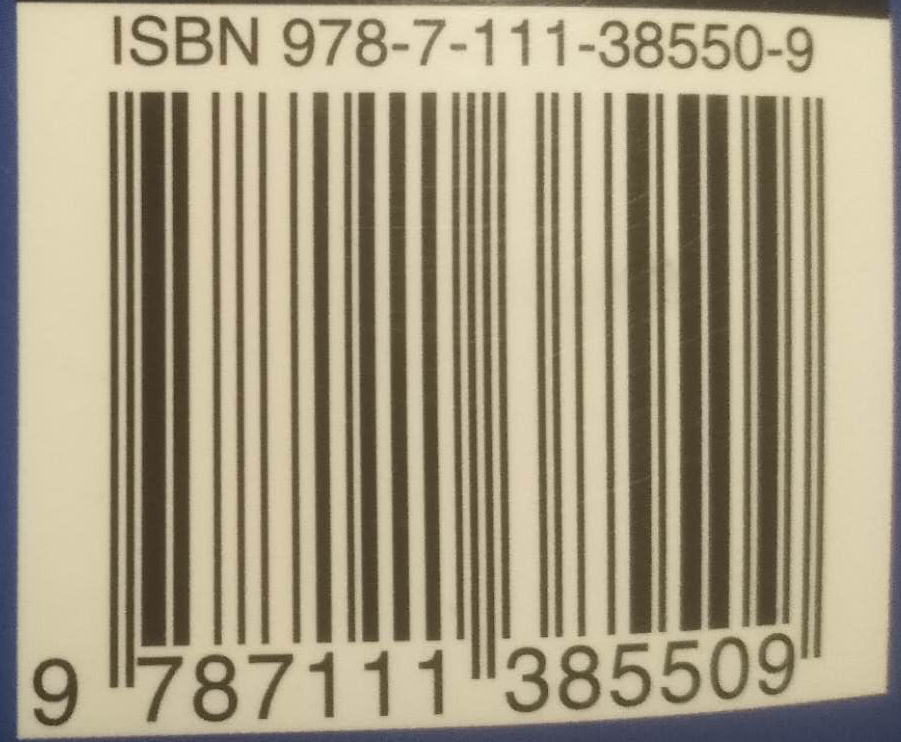
\includegraphics[width=0.4\textwidth]{isbn-13.png}
    \caption{ISBN-13 结构示例}
    \label{fig:isbn-13}
\end{figure}

\begin{method}[ISBN-13 校验码计算]
设 $13$ 位 ISBN 为 $x_1 x_2 \ldots x_{13}$，则校验码 $x_{13}$ 满足
\[
(x_1 + 3x_2 + x_3 + 3x_4 + x_5 + 3x_6 + x_7 + 3x_8 + x_9 + 3x_{10} + x_{11} + 3x_{12} + x_{13}) \equiv 0 \pmod{10}.
\]
即
\[
x_{13} \equiv (-x_1 - 3x_2 - x_3 - 3x_4 - x_5 - 3x_6 - x_7 - 3x_8 - x_9 - 3x_{10} - x_{11} - 3x_{12}) \pmod{10}.
\]
\end{method}

\begin{example}[ISBN 校验码验证]
对 ISBN 978-7-111-38550-9，验证校验码：
\begin{align*}
&-(9 + 3 \times 7 + 8 + 3 \times 7 + 1 + 3 \times 1 + 1 + 3 \times 3 + 8 + 3 \times 5 + 5 + 3 \times 0) \pmod{10}\\
&= -(9 + 21 + 8 + 21 + 1 + 3 + 1 + 9 + 8 + 15 + 5 + 0) \pmod{10}\\
&= -101 \pmod{10} = 9.
\end{align*}
与末位 $x_{13}=9$ 一致，校验通过。
\end{example}

\subsection{错误检测能力}

\begin{theorem}[单一数字错误检测]
ISBN-13 校验码可以检测\textbf{单一数字错误}（single error），即任意一位数字被错误修改的情况。

\textbf{证明思路}：设正确的 ISBN 为 $x_1\ldots x_{13}$，第 $j$ 位被改为 $(x_j + a) \bmod 10$（$1 \le a \le 9$）。
\begin{itemize}
    \item 若 $j$ 为奇数，加权和的变化量为 $a \not\equiv 0 \pmod{10}$，故校验和不整除 $10$。
    \item 若 $j$ 为偶数，加权和的变化量为 $3a \not\equiv 0 \pmod{10}$（因 $3a \in \{3,6,9,12,15,18,21,24,27\}$，均不被 $10$ 整除），故校验和不整除 $10$。
\end{itemize}
因此单一数字错误必被检出。
\end{theorem}

\begin{theorem}[换位错误检测]
ISBN-13 校验码可以检测\textbf{换位错误}（transposition error），即相邻两位数字被互换的情况，但存在例外。

\textbf{证明思路}：设相邻位 $x_j$ 与 $x_{j+1}$ 被互换。
\begin{itemize}
    \item 若 $j$ 为奇数，原贡献为 $x_j + 3x_{j+1}$，互换后为 $x_{j+1} + 3x_j$，差值为
    \[
    (x_{j+1} + 3x_j) - (x_j + 3x_{j+1}) = 2(x_j - x_{j+1}).
    \]
    \item 若 $j$ 为偶数，原贡献为 $3x_j + x_{j+1}$，互换后为 $3x_{j+1} + x_j$，差值为
    \[
    (3x_{j+1} + x_j) - (3x_j + x_{j+1}) = 2(x_{j+1} - x_j).
    \]
\end{itemize}
当 $|x_j - x_{j+1}| = 5$ 时，$2(x_j - x_{j+1}) = \pm 10 \equiv 0 \pmod{10}$，此时\textbf{无法检测}该换位错误。例如 $...38...$ 与 $...83...$ 互换时校验和不变。
\end{theorem}

%====================================================
\section{回顾（Recap）}
%====================================================

\begin{table}[htbp]
\centering
\small
\setlength{\tabcolsep}{4pt}
\begin{tabular}{|p{2.6cm}|p{11.2cm}|}
\hline
\textbf{主题} & \textbf{核心内容} \\
\hline
中国剩余定理 & 设 $m_1,\ldots,m_n>1$ 两两互素，则 $x\equiv a_i\pmod{m_i}$ 在模 $M=m_1\cdots m_n$ 下有唯一解。 \\
\hline
回代法 & 迭代合并：$x\equiv r\pmod c$，$s\equiv\bar c(a_i-r)\pmod{m_i}$，更新 $r\leftarrow cs+r$，$c\leftarrow c\cdot m_i$。 \\
\hline
大整数运算 & 剩余表示 $a\leftrightarrow(a\bmod m_1,\ldots,a\bmod m_n)$；分量-wise 加/乘可并行，再由 CRT 解码。 \\
\hline
费马小定理 & $p$ 素数且 $p\nmid a$ 时，$a^{p-1}\equiv 1\pmod p$；模幂快速计算：$a^n\bmod p=a^{n\bmod(p-1)}\bmod p$。 \\
\hline
原始根 & 模 $p$ 原始根 $r$：其幂 $r^1,\ldots,r^{p-1}$ 遍历 $\mathbb{Z}_p$ 全部非零元；每个素数模下原始根存在。 \\
\hline
离散对数 & $r^e\equiv a\pmod p$ 时，$e=\log_r a\pmod p$。 \\
\hline
哈希函数 & $h(k)=k\bmod m$；冲突用线性探测等策略解决。 \\
\hline
伪随机数 & 线性同余法 $x_{n+1}=(ax_n+c)\bmod m$；纯乘数生成器（$c=0$）如 $m=2^{31}-1,\ a=7^5$。 \\
\hline
校验码 & ISBN-13：加权和 $(x_1+3x_2+x_3+3x_4+\cdots+x_{13})\equiv 0\pmod{10}$；可检测单一错误，换位错误除差为 $5$ 外均可检测。 \\
\hline
\end{tabular}
\end{table}

%====================================================
\section{作业}
%====================================================

\begin{enumerate}
    \item \textbf{Section 4.4}
    \begin{itemize}
        \item Page 301: Exercise 20
        \item Page 302: Exercise 28
        \item Page 302: Exercise 38
    \end{itemize}
    \item \textbf{Section 4.5}
    \begin{itemize}
        \item Page 310: Exercise 34
    \end{itemize}
\end{enumerate}

\textbf{交作业时间}：奇数周周一上课前（两周交一次）。\\
\textbf{交作业方式}（二选一）：
\begin{itemize}
    \item 通过 \url{https://mooc.ucas.edu.cn/portal} 课程网站提交
    \item 上课现场提交
\end{itemize}
\textbf{答疑}：助教崔乐天、刘易铖。

\textbf{下次课程}：求解线性齐次递推关系（Solving Linear Homogeneous Recurrence Relations）。

%====================================================
% 本章术语表（更新版）
%====================================================
\newpage
\section*{术语表（本章关键术语中英对照）}
\addcontentsline{toc}{section}{术语表（本章关键术语中英对照）}

\begin{longtable}{|p{4.8cm}|p{4.8cm}|p{4.8cm}|}
\caption{数论章节关键术语中英对照表} \label{tab:number-theory} \\
\hline
\textbf{中文} & \textbf{英文} & \textbf{备注} \\
\hline
\endfirsthead

\multicolumn{3}{c}{{\tablename\ \thetable\ （续）}} \\
\hline
\textbf{中文} & \textbf{英文} & \textbf{备注} \\
\hline
\endhead

\hline
\multicolumn{3}{r}{续下页} \\
\endfoot

\hline
\endlastfoot

数论 & Number theory & 研究整数及其性质的数学分支 \\
整除 & Divisibility & $a\mid b$ 表示 $a$ 整除 $b$ \\
因子 & Factor & 整除 $b$ 的数 $a$ \\
约数 & Divisor & 同因子 \\
倍数 & Multiple & 被 $a$ 整除的数 $b$ \\
带余除法 & Division Algorithm & $a=dq+r,\ 0\le r < d$ \\
被除数 & Dividend & $a$ \\
除数 & Divisor & $d$ \\
商 & Quotient & $q=a\,\mathbf{div}\,d$ \\
余数 & Remainder & $r=a\,\mathbf{mod}\,d$ \\
下取整 & Floor function & $\lfloor a/d\rfloor$ \\
模运算 & Modular arithmetic & 只关心余数的运算 \\
同余 & Congruence & $a\equiv b\pmod{m}$ \\
模数 & Modulus & $m$ \\
不同余 & Not congruent & $a\not\equiv b\pmod{m}$ \\
消去律 & Cancellation law & 同余式两边消去公因子 \\
模 $m$ 剩余类 & Residue classes modulo $m$ & $\mathbb{Z}_m=\{0,1,\dots,m-1\}$ \\
模 $m$ 加法 & Addition modulo $m$ & $+_m$ \\
模 $m$ 乘法 & Multiplication modulo $m$ & $\cdot_m$ \\
封闭性 & Closure & 运算结果仍在集合内 \\
结合律 & Associativity & $(x\circ y)\circ z=x\circ(y\circ z)$ \\
交换律 & Commutativity & $x\circ y=y\circ x$ \\
单位元 & Identity element & 加法的 $0$，乘法的 $1$ \\
加法逆元 & Additive inverse & $a+_m(m-a)=0$ \\
分配律 & Distributivity & 乘法对加法的分配 \\
基数 & Base & 进制的底 $b$ \\
Base-$b$ 展开 & Base-$b$ expansion & $(a_k\dots a_0)_b$ \\
十进制 & Decimal & base 10 \\
二进制 & Binary & base 2 \\
八进制 & Octal & base 8 \\
十六进制 & Hexadecimal & base 16 \\
进制转换 & Base conversion & 不同进制间的互化 \\
最大公约数 & Greatest common divisor (GCD) & $\gcd(a,b)$ \\
公因子 & Common divisor & 同时整除 $a$ 和 $b$ 的正整数 \\
互素 & Relatively prime / Coprime & $\gcd(a,b)=1$ \\
两两互素 & Pairwise relatively prime & 任意两数之间均互素 \\
符号不变性 & Sign invariance & $\gcd(a,b)=\gcd(\pm a,\pm b)$ \\
\hline
贝祖定理 & Bézout's Theorem & $\gcd(a,b)=sa+tb$ \\
贝祖恒等式 & Bézout's identity & $sa+tb=\gcd(a,b)$ \\
贝祖系数 & Bézout's coefficients & 满足恒等式的整数对 $(s,t)$ \\
扩展欧几里得算法 & Extended Euclidean algorithm & 计算贝祖系数的算法 \\
良序原理 & Well-ordering property & 非空自然数子集有最小元 \\
\hline
素数 & Prime & 大于 $1$ 且只有 $1$ 和自身两个正因子 \\
合数 & Composite & 大于 $1$ 且不是素数的正整数 \\
素数定理 & Prime number theorem & $\pi(x)\sim x/\ln x$ \\
哥德巴赫猜想 & Goldbach's conjecture & 偶数表为两素数之和 \\
孪生素数猜想 & Twin prime conjecture & 存在无穷多对差为 $2$ 的素数 \\
素性测试 & Primality test & 判断整数是否为素数 \\
AKS 算法 & AKS primality test & 确定性多项式时间素性测试 \\
梅森素数 & Mersenne prime & 形如 $2^p-1$ 的素数 \\
GIMPS & Great Internet Mersenne Prime Search & 互联网梅森素数大搜索项目 \\
公钥密码学 & Public-key cryptography & 基于大整数分解困难性的密码体系 \\
\hline
算术基本定理 & Fundamental theorem of arithmetic & 素因子分解的存在唯一性 \\
素因子分解 & Prime factorization & 将整数表为素数幂的乘积 \\
欧几里得引理 & Euclid's lemma & 素数整除乘积则整除某因子 \\
存在性 & Existence & 分解的存在性证明 \\
唯一性 & Uniqueness & 分解的唯一性证明 \\
归纳基础 & Inductive basis & 数学归纳法的第一步 \\
归纳步骤 & Inductive step & 数学归纳法的递推步骤 \\
\hline
试除法 & Trial division & 通过测试不超过 $\sqrt{n}$ 的因子判断素性 \\
素性测试 & Primality test & 判断整数是否为素数的算法 \\
试除法素性测试 & Trial division primality test & 复杂度 $O(\sqrt{n}(\log n)^2)$ 位运算 \\
位运算 & Bit operation & 复杂度分析中的基本单位 \\
埃拉托色尼筛法 & Sieve of Eratosthenes & 求不超过 $n$ 的所有素数的古典算法 \\
筛法 & Sieve method & 通过筛去合数枚举素数的方法 \\
素数计数函数 & Prime counting function & $\pi(n)$，不超过 $n$ 的素数个数 \\
素数定理 & Prime number theorem (PNT) & $\pi(n)\sim n/\ln n$ \\
初等证明 & Elementary proof & 不依赖复分析的证明（Erdős, Selberg） \\
显式界 & Explicit bound & 对 $p_n$ 的上下界精确估计 \\
哈达马 & Jacques Hadamard & 法国数学家，1896年证明素数定理 \\
德·拉·瓦莱·普桑 & Charles-Jean de la Vallée Poussin & 比利时数学家，1896年证明素数定理 \\
勒让德 & Adrien-Marie Legendre & 法国数学家，素数定理猜想者之一 \\
梅森 & Marin Mersenne & 法国数学家，梅森素数以其命名 \\
\hline
欧几里得算法 & Euclidean algorithm & 高效计算最大公约数的经典算法，载于《几何原本》 \\
回代法 & Backward substitution & 从欧几里得算法递推式反解贝祖系数的方法 \\
贝祖系数 & Bézout's coefficients & 满足 $\gcd(a,b)=sa+tb$ 的整数对 $(s,t)$ \\
扩展欧几里得算法 & Extended Euclidean algorithm & 同时求 $\gcd$ 与贝祖系数的算法 \\
迭代次数 & Number of iterations & 欧几里得算法至多 $O(\log b)$ 次循环 \\
位运算复杂度 & Bit complexity & $O(\log a(\log b)^2)$ 位运算 \\
最小公倍数 & Least common multiple (LCM) & $\lcm(a,b)$，能被 $a,b$ 整除的最小正整数 \\
素因子分解法 & Prime factorization method & 通过 $\max(a_i,b_i)$ 计算 $\lcm$ \\
最大公约数与最小公倍数关系 & GCD-LCM relation & $ab=\gcd(a,b)\cdot\lcm(a,b)$ \\
同余方程 & Congruence equation & $f(x)\equiv 0\pmod m$ 形式的方程 \\
线性同余方程 & Linear congruence equation & $ax\equiv b\pmod m$ 形式的方程 \\
孙子算经 & Sunzi Suanjing & 中国古代数学经典，提出中国剩余定理问题 \\
\hline
线性同余方程 & Linear congruence equation & $ax\equiv b\pmod m$ \\
模逆元 & Inverse modulo $m$ & 满足 $\bar{a}a\equiv 1\pmod m$ 的整数 $\bar{a}$ \\
逆元存在性 & Existence of inverse & $\gcd(a,m)=1$ 时逆元存在且模 $m$ 唯一 \\
扩展欧几里得算法 & Extended Euclidean algorithm & 一趟法同时求 $\gcd$ 与贝祖系数 \\
前向过程 & Forward pass & 欧几里得算法的递推除法过程 \\
回代过程 & Backward substitution & 从递推式反解贝祖系数的过程 \\
一趟法 & One-pass method & 同步维护系数的扩展欧几里得算法 \\
互素情形 & Relatively prime case & $\gcd(a,m)=1$ 时的同余方程求解 \\
非互素情形 & Non-relatively prime case & $\gcd(a,m)>1$ 时的同余方程求解 \\
可解性条件 & Solvability condition & $d=\gcd(a,m)\mid b$ 时方程有解 \\
约化方程 & Reduced equation & $a'x\equiv b'\pmod{m'}$，其中 $a'=a/d,\ m'=m/d,\ b'=b/d$ \\
RSA加密算法 & RSA encryption algorithm & 基于模运算与素数分解困难性的公钥密码体制 \\
哥德尔不完备性定理 & Gödel's incompleteness theorems & 数理逻辑中关于形式系统局限性的里程碑定理 \\
多距离模糊分辨 & Multiple range ambiguity resolution & 雷达系统中利用中国剩余定理的技术 \\
埃拉托色尼筛法伪代码 & Sieve of Eratosthenes pseudocode & 算法实现练习 \\
\hline
中国剩余定理 & Chinese Remainder Theorem (CRT) & 孙子定理，两两互素模数下同余方程组有唯一解 \\
两两互素 & Pairwise relatively prime & 任意两个数的最大公约数为 $1$ \\
同余方程组 & System of congruence equations & 多个同余方程联立 \\
模 $M$ 唯一解 & Unique solution modulo $M$ & $M=m_1\cdots m_n$ \\
构造性证明 & Constructive proof & 显式给出解的表达式 \\
乘法逆元 & Multiplicative inverse & $\bar{a}\,a \equiv 1 \pmod{m}$ \\
回代法 & Back substitution & 逐次合并同余方程的迭代算法 \\
剩余表示 & Residue representation & 大整数用各模数下的余数向量表示 \\
并行计算 & Parallel computation & 各分量独立同时运算 \\
大整数运算 & Arithmetic with large integers & 超出机器字长的整数运算 \\
分量-wise 运算 & Component-wise operation & 按向量各分量分别运算 \\
编码 / 解码 & Encoding / Decoding & 剩余表示与常规表示的转换 \\
\hline
费马小定理 & Fermat's Little Theorem & $a^{p-1}\equiv 1\pmod p$（$p$ 素数，$p\nmid a$） \\
原始根 & Primitive root & 模 $p$ 下其幂遍历所有非零剩余类 \\
离散对数 & Discrete logarithm & $\log_r a\pmod p$，求幂指数 $e$ 使 $r^e\equiv a$ \\
哈希函数 & Hash function & 将任意数据映射到固定大小的值 \\
冲突 / 碰撞 & Collision & 不同输入映射到相同哈希值 \\
线性探测 & Linear probing & 冲突解决策略之一 \\
伪随机数 & Pseudorandom number & 确定性算法生成的近似随机序列 \\
硬件随机数生成器 & Hardware random number generator & 基于物理噪声的真随机源 \\
线性同余生成器 & Linear congruential generator & $x_{n+1}=(ax_n+c)\bmod m$ \\
种子 & Seed & 伪随机数序列的初始值 \\
\hline
线性同余法 & Linear congruential method & 最常用的伪随机数生成方法 \\
模数 & Modulus & 参数 $m$ \\
乘数 & Multiplier & 参数 $a$ \\
增量 & Increment & 参数 $c$ \\
种子 & Seed & 初始值 $x_0$ \\
纯乘数生成器 & Pure multiplier generator & $c=0$ 的线性同余法 \\
周期 & Period & 序列开始重复前的长度 \\
校验码 & Check digit & 用于检测数字串错误的附加位 \\
国际标准书号 & International Standard Book Number (ISBN) & 13位，末位为校验码 \\
单一数字错误 & Single error & 某一位数字被错误修改 \\
换位错误 & Transposition error & 相邻两位数字被互换 \\
加权和 & Weighted sum & 各位乘以特定权重后求和 \\
错误检测 & Error detection & 校验码的核心功能 \\
线性齐次递推关系 & Linear homogeneous recurrence relation & 下次课程内容 \\
\hline
\end{longtable}

\newpage
%====================================================
\chapter{高级计数技巧（Advanced Counting Techniques）}
%====================================================

\section{用递推关系计数（Counting by Recurrence Relations）}

递推关系（recurrence relations）是离散数学中描述序列的重要工具。通过建立前项与后项之间的关系，我们可以刻画许多经典计数问题的结构。

\subsection{斐波那契数列与兔子问题（Fibonacci Sequence and the Rabbit Problem）}

\begin{example}[兔子繁殖问题]
假设一对新生兔子（一公一母）被放到围栏中。兔子在出生后的第二个月开始每月繁殖一对新兔子，且每对新生兔子都遵循同样的规律。问：第 $n$ 个月时围栏中共有多少对兔子？

\textbf{递推建模}：
\begin{itemize}
    \item 第 $0$ 个月：$0$ 对兔子（初始状态），记 $F_0 = 0$；
    \item 第 $1$ 个月：$1$ 对新生兔子，记 $F_1 = 1$；
    \item 第 $n$ 个月（$n \ge 2$）的兔子总数等于上月兔子数 $F_{n-1}$ 加上本月新出生的兔子数。而本月新出生的兔子数等于两个月前已有的兔子数（这些兔子在当月均具备繁殖能力），即 $F_{n-2}$。
\end{itemize}

因此得到递推关系：
\[
F_0 = 0,\quad F_1 = 1,\quad F_n = F_{n-1} + F_{n-2}\ (n \ge 2).
\]
\end{example}

\begin{definition}[斐波那契数列]
由上述递推关系定义的数列 $\{F_n\}$ 称为\textbf{斐波那契数列}（Fibonacci sequence）。其前几项为：
\[
0,\ 1,\ 1,\ 2,\ 3,\ 5,\ 8,\ 13,\ 21,\ 34,\ 55,\ \dots
\]
\end{definition}

\begin{figure}[htbp]
    \centering
    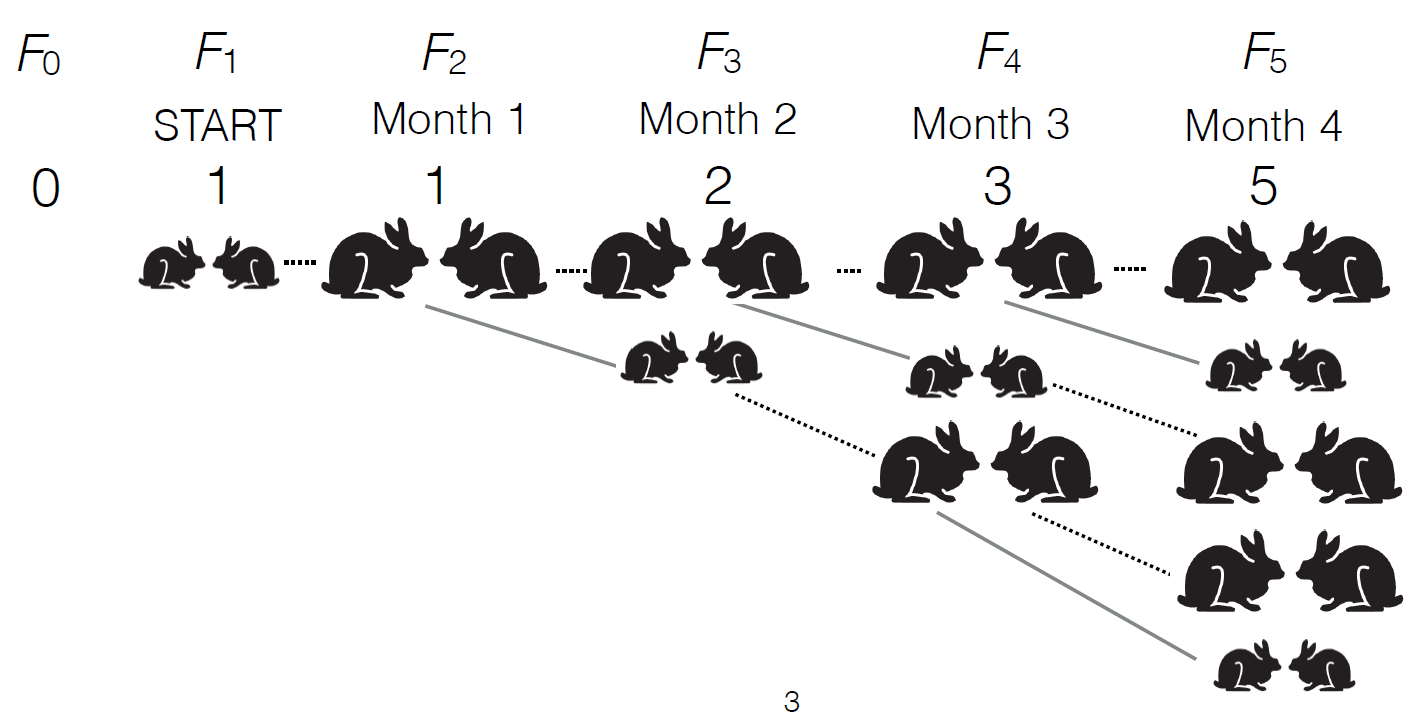
\includegraphics[width=0.7\textwidth]{fibonacci.png}
    \caption{斐波那契数列的前几项}
    \label{fig:fibonacci}
\end{figure}

\begin{property}[黄金比例]
相邻两项斐波那契数之比收敛于\textbf{黄金比例}（golden ratio）：
\[
\lim_{n \to \infty} \frac{F_{n+1}}{F_n} = \frac{1+\sqrt{5}}{2} \approx 1.618.
\]
\end{property}

\subsection{汉诺塔问题（The Tower of Hanoi）}

\begin{example}[汉诺塔]
给定三根柱子和 $n$ 个大小不同的盘片（初始时所有盘片按大小顺序叠放在第一根柱子上，大盘在下）。要求将 $n$ 个盘片全部移动到另一根柱子上，且每次只能移动一个盘片，任何时候都不能将大盘叠放在小盘之上。求完成该任务所需的\textbf{最少移动次数} $H_n$。

\textbf{递推建模}：
\begin{itemize}
    \item 当 $n=1$ 时，只需移动一次，故 $H_1 = 1$；
    \item 当 $n>1$ 时，最优策略分为三步：
        \begin{enumerate}
            \item 将上方 $n-1$ 个盘片从起始柱移到辅助柱，需 $H_{n-1}$ 次；
            \item 将最底下的第 $n$ 个盘片从起始柱移到目标柱，需 $1$ 次；
            \item 将辅助柱上的 $n-1$ 个盘片移到目标柱，需 $H_{n-1}$ 次。
        \end{enumerate}
\end{itemize}

因此得到递推关系：
\[
H_1 = 1,\quad H_n = 2H_{n-1} + 1\ (n \ge 2).
\]
\end{example}

\begin{figure}[htbp]
    \centering
    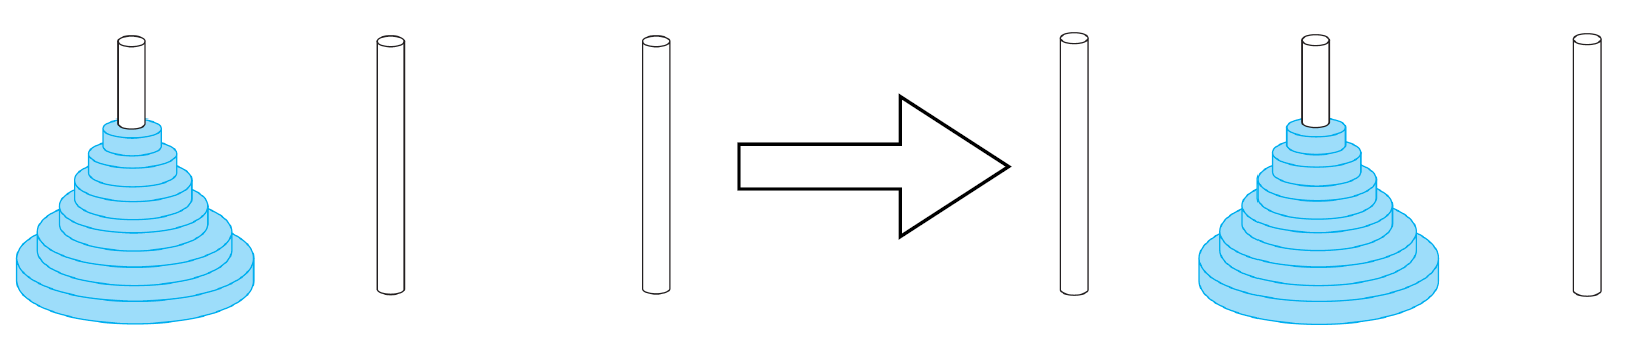
\includegraphics[width=0.8\textwidth]{hanoi.png}
    \caption{汉诺塔问题示例（$n=3$）}
    \label{fig:hanoi}
\end{figure}

\begin{property}[汉诺塔通项]
通过迭代法可求得 $H_n = 2^n - 1$。验证：
\[
2^n - 1 = 2(2^{n-1}-1)+1 = 2^n - 2 + 1 = 2^n - 1.
\]
\end{property}

\subsection{归并排序的复杂度分析（Complexity of Merge Sort）}

\begin{example}[归并排序的最坏比较次数]
设 $M_n$ 为归并排序（mergesort）对 $n$ 个元素进行排序时在最坏情况下所需的比较次数。当 $n$ 为 $2$ 的幂时，递推关系为：
\[
M_n = 2M_{n/2} + n.
\]
其中 $2M_{n/2}$ 表示对两半分别递归排序的比较次数，$+n$ 表示合并两个有序子列表所需的比较次数。
\end{example}

\begin{remark}
此类递推关系常见于\textbf{分治算法}（divide-and-conquer algorithms）。其复杂度可通过\textbf{主定理}（Master theorem）求解，结论为 $M_n = O(n \log n)$。
\end{remark}

\subsection{卡特兰数与括号化问题（Catalan Numbers and Parenthesization）}

\begin{example}[乘积的括号化]
考虑 $n+1$ 个数的乘积 $x_0 \cdot x_1 \cdot \cdots \cdot x_n$。求为该乘积添加括号以明确运算顺序的不同方式数 $C_n$。

\textbf{递推建模}：
\begin{itemize}
    \item 当 $n=0$ 时，只有一个数 $x_0$，无需括号，$C_0 = 1$；
    \item 当 $n=1$ 时，仅有一种括号方式 $(x_0 \cdot x_1)$，$C_1 = 1$；
    \item 当 $n \ge 2$ 时，最后一次乘法将序列分成左右两部分：左部分含 $i+1$ 个数（$0 \le i \le n-1$），右部分含 $n-i$ 个数。左部分有 $C_i$ 种括号化方式，右部分有 $C_{n-1-i}$ 种方式。因此：
\end{itemize}
\[
C_n = C_0 C_{n-1} + C_1 C_{n-2} + \cdots + C_{n-1} C_0 = \sum_{i=0}^{n-1} C_i C_{n-1-i}.
\]
\end{example}

\begin{definition}[卡特兰数]
由上述递推关系定义的数列 $\{C_n\}$ 称为\textbf{卡特兰数}（Catalan numbers）。其前几项为：
\[
C_0=1,\ C_1=1,\ C_2=2,\ C_3=5,\ C_4=14,\ C_5=42,\ \dots
\]
\end{definition}

\begin{remark}
卡特兰数以法国和比利时数学家 \textbf{Eugène Charles Catalan}（1814--1894）命名。该递推关系是\textbf{非线性}的，通常需要借助\textbf{生成函数}（generating functions）方法求解，其闭公式为：
\[
C_n = \frac{1}{n+1}\binom{2n}{n}.
\]
\end{remark}

%====================================================
\section{递推关系的基本概念（Basic Concepts of Recurrence Relations）}
%====================================================

\subsection{递推关系与差分方程}

\begin{remark}
递推关系（recurrence relations）在数值分析等领域也常被称为\textbf{差分方程}（difference equations）。它们与连续数学中的\textbf{微分方程}（differential equations）具有相似的哲学思想：前者处理离散输入（discrete inputs），后者处理连续输入（continuous inputs）。

\begin{table}[htbp]
\centering
\begin{tabular}{|c|c|}
\hline
\textbf{离散输入}（Discrete Inputs） & \textbf{连续输入}（Continuous Inputs） \\
\hline
差分方程 / 递推关系 & 微分方程 \\
\hline
例如：$a_n = a_{n-1} + a_{n-2}$ & 例如：$x'' = x' + 1$ \\
\hline
\end{tabular}
\end{table}
\end{remark}

\subsection{线性递推关系的定义与分类}

\begin{definition}[线性递推关系]
\textbf{线性递推关系}（linear recurrence relation）是指形如
\[
a_n = c_1 a_{n-1} + c_2 a_{n-2} + \cdots + c_k a_{n-k} + f(n)
\]
的递推式，其中：
\begin{itemize}
    \item $c_1, c_2, \dots, c_k \in \mathbb{R}$（或 $\mathbb{C}$）为\textbf{常数系数}（constant coefficients）；
    \item $k$ 称为该递推关系的\textbf{度}（degree）或\textbf{阶}（order），要求 $c_k \neq 0$；
    \item $f(n)$ 是仅依赖于 $n$ 的函数。
\end{itemize}

若 $f(n) = 0$，则称该递推关系为\textbf{齐次}（homogeneous）的；否则称为\textbf{非齐次}（nonhomogeneous）的。
\end{definition}

\begin{example}[分类示例]
\begin{table}[htbp]
\centering
\begin{tabular}{|l|l|l|}
\hline
\textbf{递推关系} & \textbf{类型} & \textbf{说明} \\
\hline
$F_n = F_{n-1} + F_{n-2}$ & 线性齐次 & 常系数，$f(n)=0$ \\
\hline
$H_n = 2H_{n-1} + 1$ & 线性非齐次 & 常系数，$f(n)=1$ \\
\hline
$a_n = a_{n-1} + a_{n-2}^2$ & 非线性 & 含平方项，非线性组合 \\
\hline
$b_n = n\,b_{n-1}$ & 线性（非常系数） & 系数 $n$ 依赖于下标 \\
\hline
\end{tabular}
\end{table}
\end{example}

\subsection{解的定义与验证}

\begin{definition}[递推关系的解]
设 $\{h_n\}$ 是一个序列。若对任意 $n \ge k$ 都有
\[
h_n = c_1 h_{n-1} + c_2 h_{n-2} + \cdots + c_k h_{n-k} + f(n),
\]
则称 $\{h_n\}$ 是该递推关系的一个\textbf{解}（solution）。
\end{definition}

\begin{example}[验证解]
\begin{itemize}
    \item 序列 $\{2^n\}$ 是 $a_n = 2a_{n-1}$ 的解，因为 $2^n = 2 \cdot 2^{n-1}$。
    \item 序列 $\{2^n - 1\}$ 是 $H_n = 2H_{n-1} + 1$ 的解，因为
    \[
    2(2^{n-1}-1)+1 = 2^n - 2 + 1 = 2^n - 1.
    \]
    \item 序列 $\{n\}$ 是 $a_n = a_{n-1} + 1$ 的解，因为 $n = (n-1) + 1$。
\end{itemize}
\end{example}

\subsection{初始条件与解的唯一性}

\begin{definition}[带初始条件的线性递推关系]
一个\textbf{带初始条件的线性递推关系}由递推式连同前 $k$ 项的初始值共同确定：
\[
\begin{cases}
a_n = c_1 a_{n-1} + c_2 a_{n-2} + \cdots + c_k a_{n-k} + f(n), \\[0.3em]
a_0 = v_0,\ a_1 = v_1,\ \dots,\ a_{k-1} = v_{k-1}.
\end{cases}
\]
\end{definition}

\begin{example}[唯一解示例]
递推关系 $a_n = 2a_{n-1}$ 在初始条件 $a_0 = 3$ 下的唯一解为 $\{3 \cdot 2^n\}$。验证：
\[
a_0 = 3 \cdot 2^0 = 3,\quad a_n = 3 \cdot 2^n = 2 \cdot (3 \cdot 2^{n-1}) = 2a_{n-1}.
\]
\end{example}

\begin{theorem}[解由初始值唯一确定]
设 $a_n = c_1 a_{n-1} + c_2 a_{n-2} + \cdots + c_k a_{n-k} + f(n)$ 是一个线性递推关系，$\{g_n\}$ 和 $\{h_n\}$ 是其两个解。则
\[
\{g_n\} = \{h_n\} \iff g_0 = h_0,\ g_1 = h_1,\ \dots,\ g_{k-1} = h_{k-1}.
\]
即两个解相等当且仅当它们的前 $k$ 个初始值完全相同。
\end{theorem}

\begin{proof}[证明思路（对 $n$ 归纳）]
\textbf{归纳基础}：由条件知 $g_i = h_i$ 对 $i = 0,1,\dots,k-1$ 成立。

\textbf{归纳步骤}：假设对所有 $n' < n$（其中 $n \ge k$）都有 $g_{n'} = h_{n'}$。则由递推关系：
\[
g_n = c_1 g_{n-1} + \cdots + c_k g_{n-k} + f(n) = c_1 h_{n-1} + \cdots + c_k h_{n-k} + f(n) = h_n.
\]
故 $g_n = h_n$。由数学归纳法，两序列对所有 $n$ 相等。
\end{proof}

\begin{corollary}[存在唯一性]
一个带初始条件的线性递推关系有且仅有\textbf{唯一解}。
\end{corollary}

%====================================================
\section{求解线性齐次递推关系（Solving Linear Homogeneous Recurrence Relations）}
%====================================================

\subsection{解空间的线性结构}

\begin{proposition}[解的线性组合]
设 $a_n = c_1 a_{n-1} + c_2 a_{n-2} + \cdots + c_k a_{n-k}$ 是一个常系数线性齐次递推关系。若 $\{g_n\}$ 和 $\{h_n\}$ 都是它的解，则：
\begin{enumerate}
    \item $\{g_n + h_n\}$ 也是该递推关系的解；
    \item 对任意常数 $\alpha$，$\{\alpha g_n\}$ 也是该递推关系的解。
\end{enumerate}
\end{proposition}

\begin{proof}
\textbf{加法封闭性}：因为 $\{g_n\}$ 和 $\{h_n\}$ 都是解，对任意 $n \ge k$ 有
\begin{align*}
g_n &= c_1 g_{n-1} + c_2 g_{n-2} + \cdots + c_k g_{n-k},\\
h_n &= c_1 h_{n-1} + c_2 h_{n-2} + \cdots + c_k h_{n-k}.
\end{align*}
两式相加得
\[
g_n + h_n = c_1(g_{n-1}+h_{n-1}) + c_2(g_{n-2}+h_{n-2}) + \cdots + c_k(g_{n-k}+h_{n-k}),
\]
故 $\{g_n+h_n\}$ 满足递推关系。

\textbf{数乘封闭性}：对任意常数 $\alpha$，将 $g_n$ 的等式两边同乘 $\alpha$ 得
\[
\alpha g_n = c_1(\alpha g_{n-1}) + c_2(\alpha g_{n-2}) + \cdots + c_k(\alpha g_{n-k}),
\]
故 $\{\alpha g_n\}$ 也满足递推关系。
\end{proof}

\begin{corollary}[解空间是线性空间]
常系数线性齐次递推关系的全体解构成的集合在序列的加法与数乘下形成一个\textbf{线性空间}（linear space）。
\end{corollary}

%====================================================
\subsection{二阶线性齐次递推关系的求解：斐波那契数列}
%====================================================

\begin{example}[求解斐波那契数列]
求解递推关系
\[
F_n = F_{n-1} + F_{n-2},\qquad F_0 = 0,\ F_1 = 1.
\]

\textbf{第一步：忽略初始条件，寻找通解形式。}

假设解具有指数形式 $F_n = \lambda^n$（其中 $\lambda \neq 0$），代入递推关系：
\[
\lambda^n = \lambda^{n-1} + \lambda^{n-2}.
\]
两边同除以 $\lambda^{n-2}$ 得
\[
\lambda^2 = \lambda + 1.
\]

\textbf{第二步：求解特征方程。}

方程 $\lambda^2 - \lambda - 1 = 0$ 的两个根为
\[
\lambda_1 = \frac{1+\sqrt{5}}{2} \approx 1.618,\qquad \lambda_2 = \frac{1-\sqrt{5}}{2} \approx -0.618.
\]
这两个根分别满足 $\lambda_1^2 = \lambda_1 + 1$ 和 $\lambda_2^2 = \lambda_2 + 1$。

\textbf{第三步：构造通解。}

由于 $\lambda_1^n$ 和 $\lambda_2^n$ 都是解，由解空间的线性性质，对任意常数 $\alpha_1, \alpha_2$，线性组合
\[
F_n = \alpha_1 \lambda_1^n + \alpha_2 \lambda_2^n
\]
也是该递推关系的解。验证：
\begin{align*}
\alpha_1\lambda_1^n + \alpha_2\lambda_2^n
&= \alpha_1(\lambda_1^{n-1}+\lambda_1^{n-2}) + \alpha_2(\lambda_2^{n-1}+\lambda_2^{n-2})\\
&= (\alpha_1\lambda_1^{n-1}+\alpha_2\lambda_2^{n-1}) + (\alpha_1\lambda_1^{n-2}+\alpha_2\lambda_2^{n-2}).
\end{align*}

\textbf{第四步：利用初始条件确定常数。}

由 $F_0 = 0$ 和 $F_1 = 1$ 得方程组：
\[
\begin{cases}
\alpha_1 + \alpha_2 = 0,\\[0.5em]
\alpha_1\lambda_1 + \alpha_2\lambda_2 = 1.
\end{cases}
\]
由第一式得 $\alpha_2 = -\alpha_1$，代入第二式：
\[
\alpha_1(\lambda_1 - \lambda_2) = 1 \implies \alpha_1 = \frac{1}{\lambda_1-\lambda_2} = \frac{1}{\sqrt{5}}.
\]
因此
\[
\alpha_1 = \frac{1}{\sqrt{5}},\qquad \alpha_2 = -\frac{1}{\sqrt{5}}.
\]

\textbf{第五步：写出闭公式（比内公式）。}

\[
\boxed{F_n = \frac{1}{\sqrt{5}}\left(\frac{1+\sqrt{5}}{2}\right)^n - \frac{1}{\sqrt{5}}\left(\frac{1-\sqrt{5}}{2}\right)^n}
\]

\textbf{渐近分析}：由于 $|\lambda_2| < 1 < \lambda_1$，第二项随 $n$ 增大趋于 $0$，故
\[
F_n = \Theta\left(\left(\frac{1+\sqrt{5}}{2}\right)^n\right).
\]
\end{example}

\begin{figure}
    \centering
    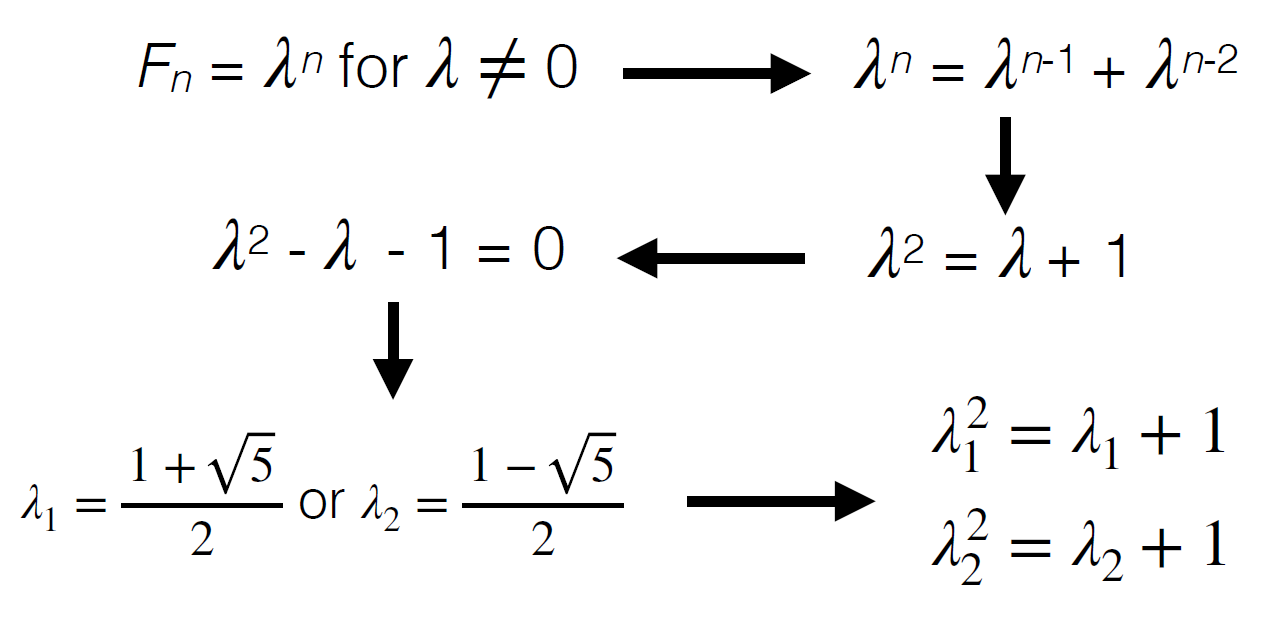
\includegraphics[width=0.7\textwidth]{fibonacci_solution.png}
    \caption{斐波那契数列通项求解示意图}
    \label{fig:fibonacci_solution}
\end{figure}

%====================================================
\subsection{特征方程与特征根}
%====================================================

\begin{definition}[特征方程与特征根]
设 $a_n = c_1 a_{n-1} + c_2 a_{n-2} + \cdots + c_k a_{n-k}$ 是一个常系数线性齐次递推关系。其\textbf{特征方程}（characteristic equation）定义为：
\[
x^k - c_1 x^{k-1} - c_2 x^{k-2} - \cdots - c_{k-1}x - c_k = 0.
\]
该方程的解称为该递推关系的\textbf{特征根}（characteristic roots）。
\end{definition}

\begin{remark}
特征方程的构造方法：将递推关系中的 $a_n$ 替换为 $x^n$，然后两边除以 $x^{n-k}$（假设 $x \neq 0$），即得：
\[
x^k = c_1 x^{k-1} + c_2 x^{k-2} + \cdots + c_k.
\]
移项后即得上式。
\end{remark}

\begin{example}[斐波那契数列的特征方程]
递推关系 $F_n = F_{n-1} + F_{n-2}$ 的特征方程为：
\[
x^2 - x - 1 = 0,
\]
其特征根为 $\displaystyle\frac{1\pm\sqrt{5}}{2}$。
\end{example}

%====================================================
\subsection{二阶情形：不同特征根}
%====================================================

\begin{theorem}[二阶不同根通解定理]
设 $a_n = c_1 a_{n-1} + c_2 a_{n-2}$（其中 $c_2 \neq 0$）是一个二阶常系数线性齐次递推关系。若其特征方程
\[
x^2 - c_1 x - c_2 = 0
\]
有两个互异（复）根 $x_1$ 和 $x_2$，则序列 $\{h_n\}$ 是该递推关系的解当且仅当存在常数 $\alpha_1, \alpha_2 \in \mathbb{C}$，使得
\[
h_n = \alpha_1 x_1^n + \alpha_2 x_2^n,\qquad \forall n \in \mathbb{N}.
\]
\end{theorem}

\begin{proof}
\textbf{充分性}（$\Leftarrow$）：已由解空间的线性性质证明——$x_1^n$ 和 $x_2^n$ 都是解，其线性组合也是解。

\textbf{必要性}（$\Rightarrow$）：设 $\{h_n\}$ 是任意解。由于递推关系由初始值 $h_0, h_1$ 唯一确定，只需证明存在 $\alpha_1, \alpha_2$ 使得
\[
\begin{cases}
\alpha_1 + \alpha_2 = h_0,\\[0.3em]
\alpha_1 x_1 + \alpha_2 x_2 = h_1.
\end{cases}
\]
该线性方程组的系数行列式为
\[
\det\begin{bmatrix}1 & 1\\ x_1 & x_2\end{bmatrix} = x_2 - x_1 \neq 0
\]
（因 $x_1 \neq x_2$），故方程组有唯一解 $(\alpha_1, \alpha_2)$。于是序列 $\{\alpha_1 x_1^n + \alpha_2 x_2^n\}$ 与 $\{h_n\}$ 满足相同的递推关系和相同的初始条件，由唯一性定理知二者恒等。
\end{proof}

\begin{figure}[htbp]
    \centering
    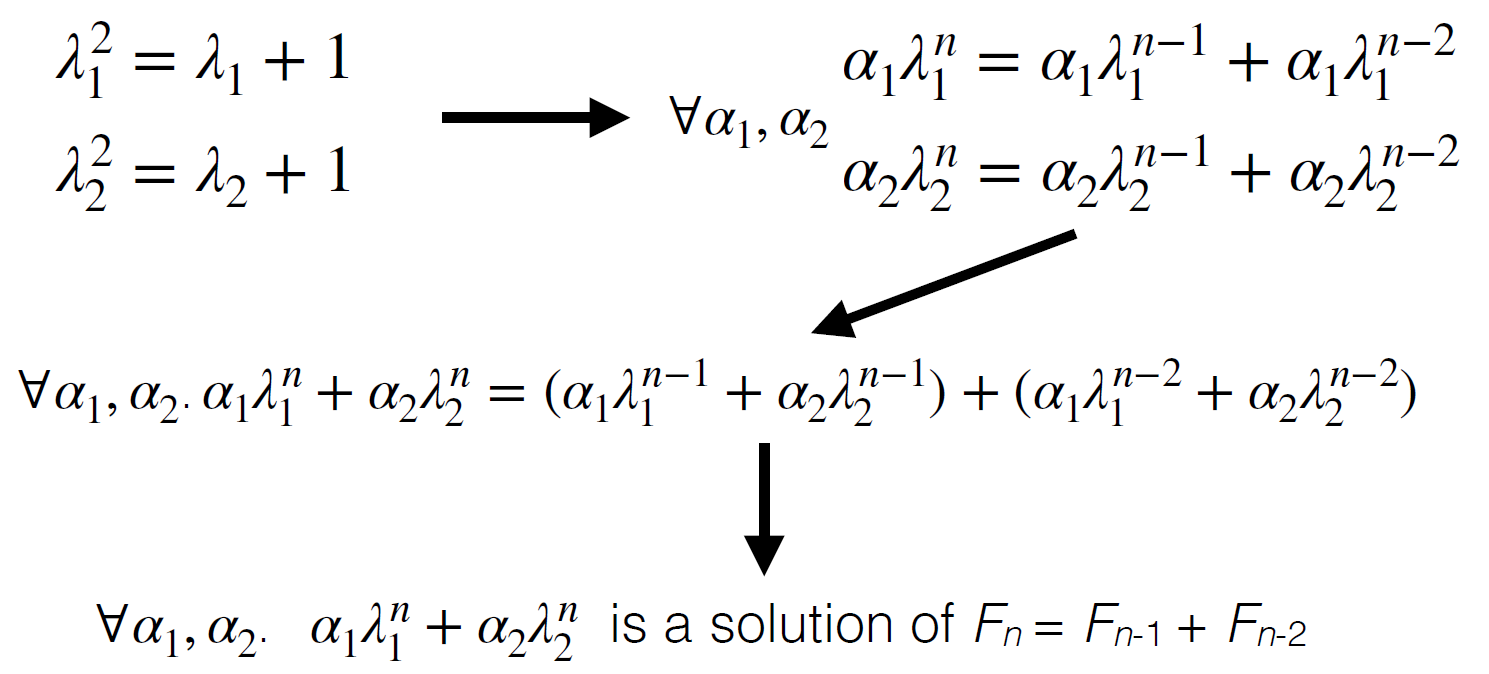
\includegraphics[width=0.8\textwidth]{distinct_roots.png}
    \caption{二阶不同特征根通解定理示意图}
    \label{fig:distinct_roots}
\end{figure}

%====================================================
\subsection{二阶情形：重根（预告）}
%====================================================

\begin{example}[重根情形预告]
考虑递推关系
\[
a_n = 6a_{n-1} - 9a_{n-2},\qquad a_0 = 1,\ a_1 = 0.
\]
其特征方程为 $x^2 - 6x + 9 = 0$，即 $(x-3)^2 = 0$，有重根 $x = 3$。

此时通解形式不再是单纯的 $\alpha_1 3^n + \alpha_2 3^n$（因为两项线性相关），需要寻找新的独立解。该情形将在后续内容中详细讨论。
\end{example}

%====================================================
\subsection{二阶情形：重根}
%====================================================

\begin{example}[二阶重根示例]
求解递推关系
\[
a_n = 6a_{n-1} - 9a_{n-2},\qquad a_0 = 1,\ a_1 = 0.
\]

\textbf{特征方程}：$x^2 - 6x + 9 = 0$，即 $(x-3)^2 = 0$，有\textbf{重根}（repeated root）$x_1 = 3$（重数为 $2$）。

此时 $3^n$ 是一个解，但通解需要另一个与之线性无关的解。可以验证 $n \cdot 3^n$ 也是该递推关系的解：
\begin{align*}
6(n-1)3^{n-1} - 9(n-2)3^{n-2}
&= 3^{n-2}\bigl[6(n-1)\cdot 3 - 9(n-2)\bigr] \\
&= 3^{n-2}\bigl[18n - 18 - 9n + 18\bigr] \\
&= 3^{n-2} \cdot 9n = n \cdot 3^n.
\end{align*}

因此通解形式为
\[
a_n = \alpha_1 \cdot 3^n + \alpha_2 \cdot n \cdot 3^n.
\]

\textbf{代入初始条件}：
\[
\begin{cases}
\alpha_1 = a_0 = 1,\\[0.3em]
3\alpha_1 + 3\alpha_2 = a_1 = 0.
\end{cases}
\]
解得 $\alpha_1 = 1,\ \alpha_2 = -1$。故
\[
a_n = 3^n - n \cdot 3^n = (1-n)3^n.
\]
\end{example}

\begin{theorem}[二阶重根通解定理]
设 $a_n = c_1 a_{n-1} + c_2 a_{n-2}$（其中 $c_2 \neq 0$）是一个二阶常系数线性齐次递推关系。若其特征方程
\[
x^2 - c_1 x - c_2 = 0
\]
只有一个（复）根 $x_1$（即重根），则序列 $\{h_n\}$ 是该递推关系的解当且仅当存在常数 $\alpha_1, \alpha_2 \in \mathbb{C}$，使得
\[
\boxed{h_n = \alpha_1 x_1^n + \alpha_2 n x_1^n,\qquad \forall n \in \mathbb{N}.}
\]
\end{theorem}

\begin{figure}[htbp]
    \centering
    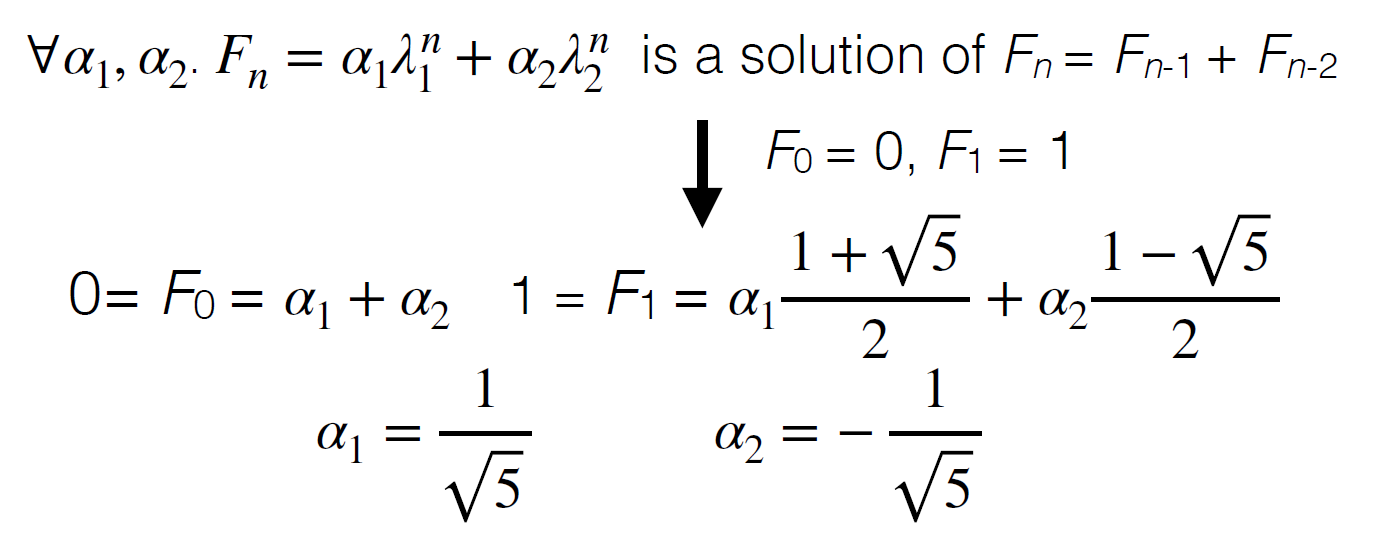
\includegraphics[width=0.8\textwidth]{repeated_root.png}
    \caption{二阶重根通解定理示意图}
    \label{fig:repeated_root}
\end{figure}

\begin{proof}[证明概要]
\textbf{充分性}：已知 $x_1^n$ 是解。验证 $n x_1^n$ 也是解：由特征方程 $x_1^2 = c_1 x_1 + c_2$，对其两边关于 $x_1$ 形式求导（或直接代入）可得
\[
n x_1^n = c_1 (n-1)x_1^{n-1} + c_2 (n-2)x_1^{n-2}
\]
在重根条件下成立。再由解空间的线性性质，线性组合也是解。

\textbf{必要性}：设 $\{h_n\}$ 为任意解。由于 $x_1 \neq 0$（否则 $c_2=0$），可令 $h_n = x_1^n b_n$。代入递推关系并利用 $x_1^2 = c_1 x_1 + c_2$ 化简，可得 $b_n$ 满足 $b_n = b_{n-1} = \cdots = b_1$，即 $b_n$ 为等差数列：$b_n = \alpha_1 + \alpha_2 n$。因此 $h_n = (\alpha_1 + \alpha_2 n)x_1^n$。
\end{proof}

%====================================================
\section{高阶线性齐次递推关系的求解}
%====================================================

\subsection{三阶及以上：不同特征根}

\begin{example}[三阶不同根示例]
求解递推关系
\[
a_n = 6a_{n-1} - 11a_{n-2} + 6a_{n-3},\qquad a_0 = 2,\ a_1 = 5,\ a_2 = 15.
\]

\textbf{特征方程}：$x^3 - 6x^2 + 11x - 6 = 0$。

因式分解得 $(x-1)(x-2)(x-3) = 0$，故三个\textbf{不同特征根}为
\[
x_1 = 1,\qquad x_2 = 2,\qquad x_3 = 3.
\]
\end{example}

\begin{theorem}[$k$ 阶不同根通解定理]
设 $a_n = c_1 a_{n-1} + c_2 a_{n-2} + \cdots + c_k a_{n-k}$（其中 $c_k \neq 0$）是一个 $k$ 阶常系数线性齐次递推关系。若其特征方程
\[
x^k - c_1 x^{k-1} - c_2 x^{k-2} - \cdots - c_k = 0
\]
有 $k$ 个互异（复）根 $x_1, x_2, \dots, x_k$，则序列 $\{h_n\}$ 是该递推关系的解当且仅当存在常数 $\alpha_1, \alpha_2, \dots, \alpha_k \in \mathbb{C}$，使得
\[
h_n = \alpha_1 x_1^n + \alpha_2 x_2^n + \cdots + \alpha_k x_k^n,\qquad \forall n \in \mathbb{N}.
\]
\end{theorem}

\begin{proof}[证明概要]
\textbf{充分性}：每个 $x_i^n$ 都满足递推关系，由解空间的线性性质，其线性组合也是解。

\textbf{必要性}：任意解 $\{h_n\}$ 由初始值 $h_0, h_1, \dots, h_{k-1}$ 唯一确定。需证明存在唯一的 $(\alpha_1,\dots,\alpha_k)$ 使得
\[
\begin{cases}
\alpha_1 + \alpha_2 + \cdots + \alpha_k = h_0,\\[0.3em]
\alpha_1 x_1 + \alpha_2 x_2 + \cdots + \alpha_k x_k = h_1,\\[0.3em]
\vdots\\[0.3em]
\alpha_1 x_1^{k-1} + \alpha_2 x_2^{k-1} + \cdots + \alpha_k x_k^{k-1} = h_{k-1}.
\end{cases}
\]
该线性方程组的系数矩阵为\textbf{范德蒙矩阵}（Vandermonde matrix）：
\[
V = \begin{bmatrix}
1 & 1 & \cdots & 1\\
x_1 & x_2 & \cdots & x_k\\
\vdots & \vdots & \ddots & \vdots\\
x_1^{k-1} & x_2^{k-1} & \cdots & x_k^{k-1}
\end{bmatrix}.
\]
其行列式为 $\det(V) = \prod_{1\le i<j\le k}(x_j - x_i) \neq 0$（因各根互异）。故方程组有唯一解，即任意解均可唯一表示为特征根幂次的线性组合。
\end{proof}

\begin{example}[三阶不同根示例续]
接上例，通解为
\[
a_n = \alpha_1 \cdot 1^n + \alpha_2 \cdot 2^n + \alpha_3 \cdot 3^n = \alpha_1 + \alpha_2 2^n + \alpha_3 3^n.
\]
代入初始条件：
\[
\begin{cases}
\alpha_1 + \alpha_2 + \alpha_3 = 2,\\[0.3em]
\alpha_1 + 2\alpha_2 + 3\alpha_3 = 5,\\[0.3em]
\alpha_1 + 4\alpha_2 + 9\alpha_3 = 15.
\end{cases}
\]
解得 $\alpha_1 = 1,\ \alpha_2 = -1,\ \alpha_3 = 2$。故
\[
a_n = 1 - 2^n + 2 \cdot 3^n.
\]
\end{example}

%====================================================
\subsection{三阶及以上：非不同特征根（重根）}
%====================================================

\begin{example}[含重根的三阶递推关系]
求解递推关系
\[
a_n = a_{n-1} + 8a_{n-2} - 12a_{n-3},\qquad a_0 = 3,\ a_1 = -2,\ a_2 = 5.
\]

\textbf{特征方程}：
\[
x^3 - x^2 - 8x + 12 = 0.
\]
因式分解得
\[
x^3 - x^2 - 8x + 12 = (x-2)^2(x+3) = 0.
\]
故有两个不同特征根：$x_1 = 2$（重数 $2$），$x_2 = -3$（重数 $1$）。
\end{example}

\begin{remark}[特征多项式的因式分解与递推关系]
上述特征多项式的因式分解 $(x-2)^2(x+3)$ 对应于以下两个低阶递推关系：
\begin{itemize}
    \item 特征方程 $(x-2)^2 = 0$ 对应 $a_n = 4a_{n-1} - 4a_{n-2}$（二阶，重根 $2$）；
    \item 特征方程 $x+3 = 0$ 对应 $a_n = -3a_{n-1}$（一阶，根 $-3$）。
\end{itemize}

可以验证：这两个低阶递推关系的解都是原递推关系的解。

\textbf{验证}（对 $a_n = 4a_{n-1} - 4a_{n-2}$ 的解）：
设 $\forall n \ge 2,\ a_n = 4a_{n-1} - 4a_{n-2}$。则对 $n \ge 3$：
\begin{align*}
&\ (a_n - 4a_{n-1} + 4a_{n-2}) + 3(a_{n-1} - 4a_{n-2} + 4a_{n-3})\\
=&\ a_n - a_{n-1} - 8a_{n-2} + 12a_{n-3} = 0.
\end{align*}
其中第一个括号内为 $0$（由假设），故原递推关系成立。

\textbf{验证}（对 $a_n = -3a_{n-1}$ 的解）：
设 $\forall n \ge 1,\ a_n = -3a_{n-1}$。则对 $n \ge 3$：
\begin{align*}
&\ (a_n + 3a_{n-1}) - 4(a_{n-1} + 3a_{n-2}) + 4(a_{n-2} + 3a_{n-3})\\
=&\ a_n - a_{n-1} - 8a_{n-2} + 12a_{n-3} = 0.
\end{align*}
其中 $a_n + 3a_{n-1} = 0$（由假设），且 $a_{n-1} + 3a_{n-2} = 0$，$a_{n-2} + 3a_{n-3} = 0$，故原递推关系成立。
\end{remark}

\begin{method}[高阶重根通解形式]
一般地，若特征方程有根 $x$ 且其重数为 $m$，则在通解中对应以下 $m$ 个线性无关的解：
\[
x^n,\quad n x^n,\quad n^2 x^n,\quad \dots,\quad n^{m-1} x^n.
\]
即重根 $x$（重数 $m$）贡献的通解部分为
\[
(\alpha_0 + \alpha_1 n + \alpha_2 n^2 + \cdots + \alpha_{m-1} n^{m-1}) x^n.
\]
\end{method}

\begin{example}[含重根的三阶递推关系续]
接上例，特征根 $2$（重数 $2$）贡献 $2^n$ 和 $n \cdot 2^n$；特征根 $-3$（重数 $1$）贡献 $(-3)^n$。故通解为
\[
a_n = \alpha_1 \cdot 2^n + \alpha_2 \cdot n \cdot 2^n + \alpha_3 \cdot (-3)^n.
\]

代入初始条件：
\[
\begin{cases}
\alpha_1 + \alpha_3 = 3,\\[0.3em]
2\alpha_1 + 2\alpha_2 - 3\alpha_3 = -2,\\[0.3em]
4\alpha_1 + 8\alpha_2 + 9\alpha_3 = 5.
\end{cases}
\]
解得 $\alpha_1 = 2,\ \alpha_2 = -\dfrac{3}{2},\ \alpha_3 = 1$。故
\[
a_n = 2^{n+1} - \frac{3}{2}n \cdot 2^n + (-3)^n.
\]
\end{example}

\begin{example}[含重根的三阶递推关系（续）]
接上例，特征根 $2$（重数 $2$）贡献 $2^n$ 和 $n \cdot 2^n$；特征根 $-3$（重数 $1$）贡献 $(-3)^n$。故通解为
\[
a_n = \alpha_1 \cdot 2^n + \alpha_2 \cdot n \cdot 2^n + \alpha_3 \cdot (-3)^n.
\]

\textbf{代入初始条件}：
\[
\begin{cases}
\alpha_1 + \alpha_3 = 3,\\[0.3em]
2\alpha_1 + 2\alpha_2 - 3\alpha_3 = -2,\\[0.3em]
4\alpha_1 + 8\alpha_2 + 9\alpha_3 = 5.
\end{cases}
\]
解得 $\alpha_1 = 2,\ \alpha_2 = -\dfrac{3}{2},\ \alpha_3 = 1$。故唯一解为
\[
a_n = 2 \cdot 2^n - \frac{3}{2} n \cdot 2^n + (-3)^n = 2^{n+1} - \frac{3}{2}n \cdot 2^n + (-3)^n.
\]
\end{example}

%====================================================
\subsection{一般情形：高阶重根的完整刻画}
%====================================================

\begin{theorem}[高阶重根通解定理]
设 $a_n = c_1 a_{n-1} + c_2 a_{n-2} + \cdots + c_k a_{n-k}$（其中 $c_k \neq 0$）是一个 $k$ 阶常系数线性齐次递推关系。设其特征方程
\[
x^k - c_1 x^{k-1} - c_2 x^{k-2} - \cdots - c_k = 0
\]
有 $t$ 个互异（复）根 $x_1, x_2, \dots, x_t$，其重数分别为 $m_1, m_2, \dots, m_t$（满足 $m_1 + m_2 + \cdots + m_t = k$）。则序列 $\{h_n\}$ 是该递推关系的解当且仅当存在常数 $\alpha_{i,j} \in \mathbb{C}$（$1 \le i \le t,\ 0 \le j < m_i$），使得
\[
\boxed{h_n = \sum_{i=1}^{t}\sum_{j=0}^{m_i-1} \alpha_{i,j}\, n^j x_i^n,\qquad \forall n \in \mathbb{N}.}
\]
\end{theorem}

\begin{remark}
该定理统一了所有情形：
\begin{itemize}
    \item 若所有根都是单根（$m_i=1$），则退化为 $h_n = \sum_{i=1}^k \alpha_i x_i^n$；
    \item 若只有一个根 $x_1$（$t=1,\ m_1=k$），则 $h_n = \sum_{j=0}^{k-1} \alpha_{1,j} n^j x_1^n$；
    \item 二阶重根情形 $h_n = \alpha_1 x_1^n + \alpha_2 n x_1^n$ 是该定理的特例。
\end{itemize}
\end{remark}

\begin{proof}[证明概要]
特征多项式可因式分解为
\[
x^k - c_1 x^{k-1} - \cdots - c_k = (x-x_1)^{m_1}(x-x_2)^{m_2}\cdots(x-x_t)^{m_t}.
\]

\textbf{情形1：$t=1$（仅一个不同根）}。此时特征方程为 $(x-x_1)^k=0$。

\textit{充分性}（``If''方向）：由引理可知，对每个 $0 \le j < k$，$n^j x_1^n$ 都是解。再由解空间的线性性质，其线性组合也是解。

\textit{必要性}（``Only if''方向）：设 $\{h_n\}$ 为任意解。构造基序列
\[
(\theta_j)_n = \begin{cases}
\dbinom{n}{j} x_1^{n-j}, & n \ge j,\\[0.5em]
0, & \text{否则}.
\end{cases}
\]
可证明任意解均可唯一表示为这些基序列的线性组合，进而化为 $n^j x_1^n$ 的线性组合。

\textbf{情形2：$t>1$（多个不同根）}。

\textit{充分性}：对每个 $i$，由情形1知 $n^j x_i^n$（$0 \le j < m_i$）是子递推关系
\[
a_n + b_{i,1} a_{n-1} + \cdots + b_{i,m_i} a_{n-m_i} = 0
\]
的解，其中 $(x-x_i)^{m_i} = x^{m_i} + b_{i,1}x^{m_i-1} + \cdots + b_{i,m_i}$。再由引理，这些解也是原递推关系的解。

\textit{必要性}：利用\textbf{广义范德蒙矩阵}（generalized Vandermonde matrix）证明初始条件可唯一确定系数。该矩阵的行列式为
\[
\prod_{1 \le j < i \le t} (x_i - x_j)^{m_i m_j} \neq 0
\]
（因各根互异），故系数存在且唯一。
\end{proof}

\begin{figure}[htbp]
    \centering
    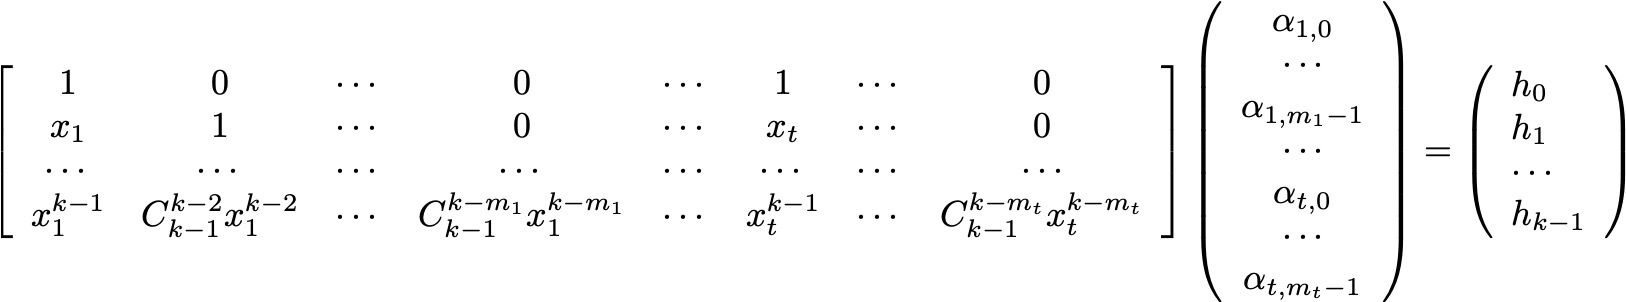
\includegraphics[width=0.8\textwidth]{generalized_vandermonde.png}
    \caption{广义范德蒙矩阵结构示意图}
    \label{fig:generalized_vandermonde}
\end{figure}

\begin{remark}
详细证明可参考：Saber Elaydi, \textit{An Introduction to Difference Equations}, 3rd edition, Undergraduate Texts in Mathematics, Springer, 2005. 第2章。
\end{remark}

%====================================================
\section*{本章总结（Recap）}
\addcontentsline{toc}{section}{本章总结}
%====================================================

\begin{itemize}
    \item \textbf{递推关系计数}：斐波那契数列、汉诺塔、归并排序、卡特兰数等经典问题均可建模为递推关系。
    \item \textbf{线性递推关系}：度为 $k$、常系数、齐次/非齐次。
    \item \textbf{解空间是线性空间}：解的线性组合仍是解。
    \item \textbf{特征方程法}：假设 $a_n = \lambda^n$，导出特征方程，求特征根。
    \item \textbf{二阶不同根}：$h_n = \alpha_1 x_1^n + \alpha_2 x_2^n$。
    \item \textbf{二阶重根}：$h_n = \alpha_1 x_1^n + \alpha_2 n x_1^n$。
    \item \textbf{$k$ 阶不同根}：$h_n = \sum_{i=1}^k \alpha_i x_i^n$。
    \item \textbf{一般情形（重根）}：$h_n = \sum_{i=1}^{t}\sum_{j=0}^{m_i-1} \alpha_{i,j} n^j x_i^n$。
\end{itemize}

%====================================================
\section*{作业}
\addcontentsline{toc}{section}{作业}
%====================================================

\begin{enumerate}
    \item 教材第8.2节：第551页，练习4(f)(g)，练习18。
    \item 补充证明：完成Lemma 1证明中的归纳步骤。\\
    \textbf{Lemma 1}：设 $a_n + b_1 a_{n-1} + \cdots + b_m a_{n-m} = 0$ 的特征方程为 $(x-d)^m = 0$。则对每个 $0 \le j < m$，$n^j d^n$ 都是该递推关系的解。\\
    \textbf{提示}：对 $j$ 归纳，证明
    \[
    \sum_{i=0}^m b_i (n-i)^j x^{n-i} = (x-d)^{m-j} q(x)
    \]
    对某个多项式 $q(x)$ 成立。
\end{enumerate}

\textbf{交作业时间}：奇数周周一上课前（两周交一次）。\\
\textbf{交作业方式}（二选一）：通过课程网站 \url{https://mooc.ucas.edu.cn/portal} 提交，或上课现场提交。\\
\textbf{答疑}：助教崔乐天、刘易铖。

\textbf{下次课程}：求解线性非齐次递推关系与分治递推关系（Solving Linear Nonhomogeneous and DAC Recurrence Relations）。

%====================================================
\section{求解线性非齐次递推关系（Solving Linear Nonhomogeneous Recurrence Relations）}
%====================================================

\subsection{关联齐次递推关系（Associated Homogeneous Recurrence Relations）}

\begin{definition}[关联齐次递推关系]
设
\[
a_n = c_1 a_{n-1} + c_2 a_{n-2} + \cdots + c_k a_{n-k} + f(n)
\]
是一个常系数线性非齐次递推关系，其中 $c_1,\dots,c_k\in\mathbb{R}$（或 $\mathbb{C}$），$f(n)\not\equiv 0$。将其非齐次项 $f(n)$ 去掉后得到的
\[
a_n = c_1 a_{n-1} + c_2 a_{n-2} + \cdots + c_k a_{n-k}
\]
称为该非齐次递推关系的\textbf{关联齐次递推关系}（associated homogeneous linear recurrence relation）。
\end{definition}

\begin{example}
递推关系 $H_n = 2H_{n-1} + 1$ 的关联齐次递推关系为
\[
H_n = 2H_{n-1}.
\]
\end{example}

\begin{remark}
关联齐次递推关系的解空间结构已在上一节中完整刻画：其通解由特征根决定，是 $k$ 维线性空间（在复数域上）。
\end{remark}

%====================================================
\subsection{解的结构定理（Structure Theorem for Solutions）}
%====================================================

\begin{theorem}[非齐次递推关系的解结构]\label{thm:nonhom-structure}
设
\[
a_n = c_1 a_{n-1} + c_2 a_{n-2} + \cdots + c_k a_{n-k} + f(n)
\]
是一个常系数线性非齐次递推关系，$\{h_n^{(p)}\}$ 是它的一个\textbf{特解}（particular solution）。则该递推关系的\textbf{每一个解} $\{g_n\}$ 都可以唯一地表示为
\[
g_n = h_n^{(p)} + h_n^{(q)},\qquad \forall n\in\mathbb{N},
\]
其中 $\{h_n^{(q)}\}$ 是其关联齐次递推关系的某个解。
\end{theorem}

\begin{proof}
设 $\{h_n^{(p)}\}$ 是一个特解，则对任意 $n\ge k$ 有
\[
h_n^{(p)} = c_1 h_{n-1}^{(p)} + c_2 h_{n-2}^{(p)} + \cdots + c_k h_{n-k}^{(p)} + f(n).
\tag{1}
\]

设 $\{g_n\}$ 是该非齐次递推关系的任意一个解，则对任意 $n\ge k$ 有
\[
g_n = c_1 g_{n-1} + c_2 g_{n-2} + \cdots + c_k g_{n-k} + f(n).
\tag{2}
\]

将 (2) 减去 (1)，并令 $h_n^{(q)} := g_n - h_n^{(p)}$，得到
\[
h_n^{(q)} = c_1 h_{n-1}^{(q)} + c_2 h_{n-2}^{(q)} + \cdots + c_k h_{n-k}^{(q)}.
\]
这说明 $\{h_n^{(q)}\}$ 恰好满足关联齐次递推关系。于是
\[
g_n = h_n^{(p)} + h_n^{(q)},
\]
证毕。
\end{proof}

\begin{corollary}[通解公式]
常系数线性非齐次递推关系的\textbf{通解}等于其\textbf{一个特解}加上关联齐次递推关系的\textbf{通解}：
\[
\boxed{h_n = h_n^{(p)} + h_n^{(h)}},
\]
其中 $h_n^{(h)}$ 表示齐次通解（含 $k$ 个任意常数）。
\end{corollary}

\begin{example}[汉诺塔通解的再验证]
考虑 $H_n = 2H_{n-1} + 1$。
\begin{itemize}
    \item 一个特解：可以验证常数序列 $\{-1\}$ 是特解，因为 $-1 = 2(-1) + 1$。
    \item 关联齐次递推 $H_n = 2H_{n-1}$ 的通解为 $c\cdot 2^n$。
\end{itemize}
因此通解为 $H_n = c\cdot 2^n - 1$。代入初始条件 $H_1 = 1$ 得 $c=1$，故 $H_n = 2^n - 1$，与之前结果一致。
\end{example}

%====================================================
\subsection{待定系数法求特解（Method of Undetermined Coefficients）}
%====================================================

对于一般的非齐次项 $f(n)$，没有普适的求特解方法。但当 $f(n)$ 具有特定形式——即一个关于 $n$ 的多项式乘以某个常数的 $n$ 次幂——时，可以使用\textbf{待定系数法}系统求解。

\begin{theorem}[多项式-指数型非齐次项的特解形式]\label{thm:undet-coeff}
设非齐次递推关系为
\[
a_n = c_1 a_{n-1} + \cdots + c_k a_{n-k} + f(n),
\qquad c_1,\dots,c_k\in\mathbb{R},
\]
其中非齐次项
\[
f(n) = (b_t n^t + b_{t-1} n^{t-1} + \cdots + b_1 n + b_0)\, s^n,
\quad b_t,\dots,b_0,s\in\mathbb{R},\ b_t\neq 0.
\]

\begin{enumerate}
    \item \textbf{情形一}：若 $s$ \textbf{不是}关联齐次递推关系特征方程的根，则存在一个形如
    \[
    h_n^{(p)} = (p_t n^t + p_{t-1} n^{t-1} + \cdots + p_1 n + p_0)\, s^n
    \]
    的特解，其中 $p_t,\dots,p_0$ 为待定常数。

    \item \textbf{情形二}：若 $s$ 是特征方程的根，且其\textbf{重数}为 $m$（$m\ge 1$），则存在一个形如
    \[
    h_n^{(p)} = n^m (p_t n^t + p_{t-1} n^{t-1} + \cdots + p_1 n + p_0)\, s^n
    \]
    的特解。
\end{enumerate}
\end{theorem}

\begin{proof}[证明思路]
核心思想是将特解形式代入递推关系，通过比较 $n$ 的同次幂系数来确定 $p_t,\dots,p_0$。

以情形一为例，将 $h_n^{(p)} = q(n)s^n$（其中 $q(n)$ 为 $t$ 次多项式）代入递推关系并除以 $s^{n-k}$，得到
\[
s^k q(n) = c_1 s^{k-1} q(n-1) + \cdots + c_k q(n-k) + b_t n^t + \cdots + b_0.
\]
由于 $s$ 不是特征根，$s^k - c_1 s^{k-1} - \cdots - c_k \neq 0$，左边 $q(n)$ 的最高次项 $p_t n^t$ 不会被完全抵消，因此可以通过比较系数唯一确定 $p_t,\dots,p_0$。

若 $s$ 是特征根（重数 $m$），则直接代入 $q(n)s^n$ 会导致最高次项系数方程奇异（左边最高次项被消去）。此时乘以 $n^m$ 可以恢复非奇异性，使得比较系数法仍然可行。严格的证明需要验证算子 $(E - s)^m$（其中 $E$ 为移位算子）作用于 $n^m q(n)s^n$ 后能产生 $t$ 次多项式，详见 Elaydi 或 Cull 等的差分方程教材。
\end{proof}

\begin{remark}
当 $s=1$ 时，$f(n)$ 退化为纯多项式 $b_t n^t + \cdots + b_0$。此时特解形式取决于 $1$ 是否为特征方程的根：
\begin{itemize}
    \item 若 $1$ 不是特征根，特解为同次多项式；
    \item 若 $1$ 是特征根（重数 $m$），特解为 $n^m \times$ 同次多项式。
\end{itemize}
\end{remark}

\begin{example}[含指数项的非齐次递推关系]
求解
\[
a_n = 6a_{n-1} - 9a_{n-2} + n\cdot 2^n,\qquad a_0,\ a_1\ \text{给定}.
\]

\textbf{第一步：求关联齐次通解。}

特征方程 $x^2 - 6x + 9 = 0$ 即 $(x-3)^2 = 0$，有重根 $x=3$（重数 $2$）。故齐次通解为
\[
a_n^{(h)} = (\alpha_1 + \alpha_2 n)\, 3^n.
\]

\textbf{第二步：确定特解形式。}

非齐次项 $f(n) = n\cdot 2^n$，其中 $s=2$。因为 $2$ 不是特征根（特征根只有 $3$），故设特解
\[
a_n^{(p)} = (An + B)\, 2^n.
\]

\textbf{第三步：代入求系数。}

将特解形式代入原递推关系：
\[
(An+B)2^n = 6\bigl(A(n-1)+B\bigr)2^{n-1} - 9\bigl(A(n-2)+B\bigr)2^{n-2} + n\cdot 2^n.
\]
两边除以 $2^{n-2}$ 得：
\[
4(An+B) = 12\bigl(A(n-1)+B\bigr) - 9\bigl(A(n-2)+B\bigr) + 4n.
\]
展开整理：
\[
4An + 4B = (12A - 9A + 4)n + (-12A + 12B + 18A - 9B).
\]
即
\[
4An + 4B = (3A + 4)n + (6A + 3B).
\]
比较系数：
\[
\begin{cases}
4A = 3A + 4 \implies A = 4,\\[0.3em]
4B = 6A + 3B \implies B = 24.
\end{cases}
\]
故特解为 $a_n^{(p)} = (4n + 24)\, 2^n$。

\textbf{第四步：写出通解。}

\[
a_n = (\alpha_1 + \alpha_2 n)\, 3^n + (4n + 24)\, 2^n.
\]
再由初始条件确定 $\alpha_1,\alpha_2$ 即可。
\end{example}

\begin{example}[求和型递推关系：平方和公式]
设 $a_n = \sum_{k=1}^{n} k^2$。则 $a_n$ 满足递推关系
\[
a_n = a_{n-1} + n^2,\qquad a_0 = 0.
\]

\textbf{第一步：齐次部分。}

关联齐次递推为 $a_n = a_{n-1}$，特征方程 $x - 1 = 0$，根 $x=1$（重数 $1$）。齐次通解为 $\alpha\cdot 1^n = \alpha$。

\textbf{第二步：特解形式。}

$f(n) = n^2 = n^2\cdot 1^n$，其中 $s=1$ 正是特征根（重数 $m=1$）。因此设特解
\[
a_n^{(p)} = n^1(An^2 + Bn + C) = An^3 + Bn^2 + Cn.
\]

\textbf{第三步：代入求系数。}

\[
An^3 + Bn^2 + Cn = A(n-1)^3 + B(n-1)^2 + C(n-1) + n^2.
\]
展开右边：
\begin{align*}
& A(n^3 - 3n^2 + 3n - 1) + B(n^2 - 2n + 1) + C(n-1) + n^2\\
=&\ An^3 + (-3A + B + 1)n^2 + (3A - 2B + C)n + (-A + B - C).
\end{align*}
比较两边系数：
\[
\begin{cases}
A = A & \text{（自动满足）},\\
B = -3A + B + 1 \implies 3A = 1 \implies A = \dfrac{1}{3},\\[0.5em]
C = 3A - 2B + C \implies 2B = 3A \implies B = \dfrac{1}{2},\\[0.5em]
0 = -A + B - C \implies C = B - A = \dfrac{1}{2} - \dfrac{1}{3} = \dfrac{1}{6}.
\end{cases}
\]
故特解为
\[
a_n^{(p)} = \frac{1}{3}n^3 + \frac{1}{2}n^2 + \frac{1}{6}n = \frac{n(n+1)(2n+1)}{6}.
\]

\textbf{第四步：通解与初始条件。}

通解 $a_n = \alpha + \frac{n(n+1)(2n+1)}{6}$。由 $a_0=0$ 得 $\alpha=0$。因此
\[
\boxed{\sum_{k=1}^{n} k^2 = \frac{n(n+1)(2n+1)}{6}}.
\]
\end{example}

%====================================================
\section{分治递推关系（Divide-and-Conquer Recurrence Relations）}
%====================================================

\subsection{分治算法与递推模型（Divide-and-Conquer Algorithms）}

\textbf{分治}（Divide-and-Conquer, DAC）是算法设计中的核心范式，其基本思想为：
\begin{enumerate}
    \item \textbf{分}（Divide）：将规模为 $n$ 的问题分解为若干个规模更小的子问题；
    \item \textbf{治}（Conquer）：递归地求解各子问题；
    \item \textbf{合}（Combine）：将子问题的解合并为原问题的解。
\end{enumerate}

分治算法的时间复杂度或比较次数通常可用\textbf{分治递推关系}描述，其一般形式为
\[
T(n) = a\,T(n/b) + g(n),
\]
其中 $a$ 为子问题个数，$n/b$ 为子问题规模，$g(n)$ 为分解与合并的代价。

\begin{remark}
与前面研究的常系数线性递推不同，分治递推中的 $n/b$ 通常要求 $n$ 为 $b$ 的幂次（或取整），且系数非常数（依赖于 $n$）。这类递推关系可通过\textbf{迭代展开法}（iteration/unrolling）或\textbf{主定理}（Master Theorem）求解。
\end{remark}

%====================================================
\subsection{二分搜索的比较次数分析（Binary Search）}
%====================================================

\begin{example}[二分搜索]
考虑在有序数组 $a_1 < a_2 < \cdots < a_n$ 中查找元素 $x$ 的\textbf{二分搜索}算法（binary search）：

\begin{verbatim}
procedure bsearch(x, a_1, ..., a_n):
    if n = 1 then
        if x = a_1 then return 1 else return 0
    else
        m := floor(n/2)
        if x >= a_m then
            temp := bsearch(x, a_{m+1}, ..., a_n)
            if temp > 0 then return m + temp else return 0
        else
            return bsearch(x, a_1, ..., a_m)
\end{verbatim}

设 $I(n)$ 为该算法在最坏情况下所需的\textbf{比较次数}。当 $n$ 为偶数时，每次将问题规模减半，并在划分点进行 $1$ 次比较，在合并/判断时进行额外常数次比较。简化模型为：
\[
I(n) = I(n/2) + 3,\qquad n\ \text{even},\ n\ge 2,
\]
其中常数 $3$ 来自划分点比较与返回值处理（不同教材常数可能不同，核心在于 $O(1)$ 附加项）。
\end{example}

\begin{property}[二分搜索复杂度]
通过迭代展开：
\[
I(n) = I(n/2) + 3 = I(n/4) + 3 + 3 = \cdots = I(1) + 3\log_2 n.
\]
因此 $I(n) = O(\log n)$。
\end{property}

%====================================================
\subsection{最大最小值查找的比较次数分析（Finding Maximum and Minimum）}
%====================================================

\begin{example}[同时找最大最小值]
考虑从 $n$ 个实数 $a_1,\dots,a_n$ 中同时找出最大值和最小值的\textbf{Maxmin}算法：

\begin{verbatim}
procedure Maxmin(a_1, ..., a_n):
    if n = 1 then return (a_1, a_1)
    else
        m := floor(n/2)
        (x_1, y_1) := Maxmin(a_1, ..., a_m)
        (x_2, y_2) := Maxmin(a_{m+1}, ..., a_n)
        x := max(x_1, x_2)
        y := min(y_1, y_2)
        return (x, y)
\end{verbatim}

设 $f(n)$ 为该算法在最坏情况下所需的\textbf{元素比较次数}。当 $n$ 为偶数时，算法递归处理两个规模为 $n/2$ 的子数组，然后在合并阶段进行 $2$ 次比较（一次 $\max$，一次 $\min$），加上划分时的常数开销，模型为：
\[
f(n) = 2f(n/2) + 3,\qquad n\ \text{even},\ n\ge 2.
\]
\end{example}

\begin{property}[Maxmin复杂度]
迭代展开递推关系（设 $n=2^k$）：
\begin{align*}
f(2^k) &= 2f(2^{k-1}) + 3\\
&= 2\bigl(2f(2^{k-2}) + 3\bigr) + 3 = 2^2 f(2^{k-2}) + 2\cdot 3 + 3\\
&= \cdots\\
&= 2^k f(1) + 3(2^{k-1} + 2^{k-2} + \cdots + 2 + 1)\\
&= 2^k f(1) + 3(2^k - 1).
\end{align*}
若 $f(1)=0$（$n=1$ 时无比较），则 $f(n) = 3(n-1)$，即 $f(n) = O(n)$。这比 naive 的 $2(n-1)$ 次比较更优（通过成对处理可进一步优化至 $\lceil 3n/2 \rceil - 2$）。
\end{property}

\begin{remark}
上述两个例子展示了分治递推的典型形式 $T(n) = aT(n/b) + g(n)$。当 $g(n)$ 为常数或多项式时，可通过\textbf{主定理}（Master Theorem）直接得到渐近阶：
\[
T(n) = \begin{cases}
\Theta(n^{\log_b a}), & \text{if } g(n) = O(n^{\log_b a - \varepsilon}),\\[0.3em]
\Theta(n^{\log_b a}\log n), & \text{if } g(n) = \Theta(n^{\log_b a}),\\[0.3em]
\Theta(g(n)), & \text{if } g(n) = \Omega(n^{\log_b a + \varepsilon}).
\end{cases}
\]
二分搜索对应 $a=1,b=2,g(n)=O(1)$，故 $\log_2 1 = 0$，得 $T(n)=\Theta(\log n)$；Maxmin 对应 $a=2,b=2,g(n)=O(1)$，故 $\log_2 2 = 1$，但 $g(n)$ 低于临界值，实际展开得 $T(n)=\Theta(n)$。
\end{remark}

%====================================================
\subsection{归并排序的复杂度分析（Merge Sort）}
%====================================================

\begin{example}[归并排序的比较次数递推]
归并排序（mergesort）是典型的分治排序算法，其伪代码如下：

\begin{verbatim}
procedure mergesort(L = a_1, ..., a_n):
    if n > 1 then
        m := floor(n/2)
        L1 := a_1, a_2, ..., a_m
        L2 := a_{m+1}, a_{m+2}, ..., a_n
        L := merge(mergesort(L1), mergesort(L2))
    // L 现在已按非递减顺序排好序
\end{verbatim}

设 $f(n)$ 为对 $n$ 个元素进行归并排序时在最坏情况下所需的\textbf{比较次数}。当 $n$ 为偶数时，算法将列表均分为两个规模为 $n/2$ 的子列表，递归排序后执行合并操作。合并两个已排序子列表最多需要 $n-1$ 次比较（简化为 $n$ 次）。因此递推关系为：
\[
f(n) = 2f(n/2) + n,\qquad n\ \text{even},\ n\ge 2.
\]
\end{example}

\begin{property}[归并排序复杂度]
通过迭代展开（设 $n=2^k$）：
\begin{align*}
f(2^k) &= 2f(2^{k-1}) + 2^k\\
&= 2\bigl(2f(2^{k-2}) + 2^{k-1}\bigr) + 2^k = 2^2 f(2^{k-2}) + 2\cdot 2^k\\
&= \cdots\\
&= 2^k f(1) + k\cdot 2^k.
\end{align*}
若 $f(1)=0$，则 $f(n) = n\log_2 n$，即 $f(n) = O(n\log n)$。
\end{property}

%====================================================
\subsection{快速整数乘法（Fast Multiplication of Integers）}
%====================================================

\begin{example}[朴素分治乘法]
设 $A$ 和 $B$ 是两个 $2n$ 位二进制整数。将其各分为高 $n$ 位和低 $n$ 位：
\[
A = 2^n A_1 + A_0,\qquad B = 2^n B_1 + B_0,
\]
其中 $A_1,A_0,B_1,B_0$ 均为 $n$ 位整数。则
\[
A\times B = 2^{2n}(A_1 B_1) + 2^n(A_1 B_0 + A_0 B_1) + (A_0 B_0).
\]

\textbf{复杂度分析}：上述公式需要计算 $A_1B_1, A_1B_0, A_0B_1, A_0B_0$ 共 \textbf{4 次} $n$ 位整数乘法，以及若干次移位和加法（线性时间）。设 $f(n)$ 为 $n$ 位输入所需的位运算次数，则：
\[
f(2n) = 4f(n) + Cn \quad\Longrightarrow\quad f(n) = 4f(n/2) + \Theta(n).
\]
由主定理（$a=4,b=2,d=1$，$4>2^1$）得 $f(n) = \Theta(n^{\log_2 4}) = \Theta(n^2)$，与小学竖式乘法同阶。
\end{example}

\begin{example}[Karatsuba 快速乘法]
1960 年，Anatolii Karatsuba 发现可以将 4 次乘法降为 \textbf{3 次}。关键观察是：
\[
A_1 B_0 + A_0 B_1 = (A_1 + A_0)(B_1 + B_0) - A_1 B_1 - A_0 B_0.
\]

因此只需计算以下三个乘积：
\begin{align*}
P_1 &= A_1 B_1,\\
P_2 &= A_0 B_0,\\
P_3 &= (A_1 - A_0)(B_0 - B_1) = (A_1 + A_0)(B_1 + B_0) - A_1 B_1 - A_0 B_0.
\end{align*}

原乘积可重写为：
\[
A\times B = (2^{2n} + 2^n)P_1 + 2^n P_3 + (2^n + 1)P_2.
\]

\textbf{复杂度分析}：仅需 3 次 $n$ 位乘法，递推关系变为：
\[
f(2n) = 3f(n) + Cn \quad\Longrightarrow\quad f(n) = 3f(n/2) + \Theta(n).
\]
由主定理（$a=3,b=2,d=1$，$3>2^1$）得：
\[
f(n) = \Theta(n^{\log_2 3}) \approx \Theta(n^{1.585}),
\]
显著优于朴素算法的 $\Theta(n^2)$。
\end{example}

%====================================================
\subsection{快速矩阵乘法（Fast Multiplication of Matrices）}
%====================================================

\begin{example}[矩阵乘法的朴素算法]
设 $A=[a_{ij}]$ 和 $B=[b_{ij}]$ 为两个 $n\times n$ 矩阵，其乘积 $C=A\cdot B$ 的元素为
\[
C_{ij} = \sum_{k=1}^{n} a_{ik} b_{kj}.
\]
朴素算法需要 $n^3$ 次乘法和 $n^3-n^2$ 次加法，总复杂度为 $\Theta(n^3)$。
\end{example}

\begin{example}[矩阵乘法的简单分治算法]
将 $A,B,C$ 各划分为 $2\times 2$ 的 $n/2\times n/2$ 分块矩阵：
\[
A = \begin{pmatrix} A_{11} & A_{12}\\ A_{21} & A_{22}\end{pmatrix},\quad
B = \begin{pmatrix} B_{11} & B_{12}\\ B_{21} & B_{22}\end{pmatrix},\quad
C = \begin{pmatrix} C_{11} & C_{12}\\ C_{21} & C_{22}\end{pmatrix}.
\]

则分块乘法为：
\begin{align*}
C_{11} &= A_{11}B_{11} + A_{12}B_{21},\\
C_{12} &= A_{11}B_{12} + A_{12}B_{22},\\
C_{21} &= A_{21}B_{11} + A_{22}B_{21},\\
C_{22} &= A_{21}B_{12} + A_{22}B_{22}.
\end{align*}

\textbf{复杂度分析}：需要 \textbf{8 次} $n/2$ 规模的矩阵乘法和 \textbf{4 次} $n/2$ 规模的矩阵加法（每次加法涉及 $(n/2)^2$ 个元素）。设 $f(n)$ 为 $n\times n$ 矩阵乘法所需的运算次数，则：
\[
f(n) = 8f(n/2) + 4\cdot(n/2)^2 = 8f(n/2) + n^2,\qquad n\ \text{even}.
\]
由主定理（$a=8,b=2,d=2$，$8>2^2=4$）得 $f(n) = \Theta(n^{\log_2 8}) = \Theta(n^3)$，与朴素算法同阶，分治并未带来渐进改进。
\end{example}

\begin{example}[Strassen 算法]
1969 年，德国数学家 Volker Strassen 发现可将 8 次乘法降为 \textbf{7 次}，从而突破 $\Theta(n^3)$ 的壁垒。

首先计算 10 个辅助矩阵（仅加减法）：
\begin{align*}
S_1 &= B_{12} - B_{22}, & S_6 &= B_{11} + B_{22},\\
S_2 &= A_{11} + A_{12}, & S_7 &= A_{12} - A_{22},\\
S_3 &= A_{21} + A_{22}, & S_8 &= B_{21} + B_{22},\\
S_4 &= B_{21} - B_{11}, & S_9 &= A_{11} - A_{21},\\
S_5 &= A_{11} + A_{22}, & S_{10} &= B_{11} + B_{12}.
\end{align*}

然后计算 7 个分块乘积：
\begin{align*}
P_1 &= A_{11}\cdot S_1 = A_{11}B_{12} - A_{11}B_{22},\\
P_2 &= S_2\cdot B_{22} = A_{11}B_{22} + A_{12}B_{22},\\
P_3 &= S_3\cdot B_{11} = A_{21}B_{11} + A_{22}B_{11},\\
P_4 &= A_{22}\cdot S_4 = A_{22}B_{21} - A_{22}B_{11},\\
P_5 &= S_5\cdot S_6 = A_{11}B_{11} + A_{11}B_{22} + A_{22}B_{11} + A_{22}B_{22},\\
P_6 &= S_7\cdot S_8 = A_{12}B_{21} + A_{12}B_{22} - A_{22}B_{21} - A_{22}B_{22},\\
P_7 &= S_9\cdot S_{10} = A_{11}B_{11} + A_{11}B_{12} - A_{21}B_{11} - A_{21}B_{12}.
\end{align*}

最后通过加减组合得到 $C$ 的四个分块：
\begin{align*}
C_{11} &= P_5 + P_4 - P_2 + P_6,\\
C_{12} &= P_1 + P_2,\\
C_{21} &= P_3 + P_4,\\
C_{22} &= P_5 + P_1 - P_3 - P_7.
\end{align*}

\textbf{验证}（以 $C_{11}$ 为例）：
\begin{align*}
& P_5 + P_4 - P_2 + P_6\\
=&\ (A_{11}B_{11} + A_{11}B_{22} + A_{22}B_{11} + A_{22}B_{22})\\
&\ + (A_{22}B_{21} - A_{22}B_{11}) - (A_{11}B_{22} + A_{12}B_{22})\\
&\ + (A_{12}B_{21} + A_{12}B_{22} - A_{22}B_{21} - A_{22}B_{22})\\
=&\ A_{11}B_{11} + A_{12}B_{21}.
\end{align*}
这正是 $C_{11}$ 的定义。其余三块同理可验证。

\textbf{复杂度分析}：仅需 7 次 $n/2$ 规模矩阵乘法和约 $9n^2/2$ 次加减法。递推关系为：
\[
f(n) = 7f(n/2) + \frac{9}{2}n^2,\qquad n\ \text{even}.
\]
由主定理（$a=7,b=2,d=2$，$7>2^2=4$）得：
\[
f(n) = \Theta(n^{\log_2 7}) \approx \Theta(n^{2.807}),
\]
首次将矩阵乘法复杂度降至 $O(n^{2.81})$ 以下。
\end{example}

%====================================================
\section{求解分治递推关系（Solving DAC Recurrence Relations）}
%====================================================

\subsection{迭代展开法（Iteration / Unrolling Method）}

\begin{method}[分治递推的迭代展开]
考虑标准形式的分治递推关系：
\[
f(n) = a\,f(n/b) + g(n),\qquad n\ \text{divisible by } b.
\]
设 $n = b^k$（即 $k = \log_b n$），逐层展开：
\begin{align*}
f(n) &= a\,f(n/b) + g(n)\\
&= a\bigl(a\,f(n/b^2) + g(n/b)\bigr) + g(n) = a^2 f(n/b^2) + a\,g(n/b) + g(n)\\
&= a^3 f(n/b^3) + a^2 g(n/b^2) + a\,g(n/b) + g(n)\\
&\ \vdots\\
&= a^k f(n/b^k) + \sum_{i=0}^{k-1} a^i\,g(n/b^i)\\
&= a^k f(1) + \sum_{i=0}^{k-1} a^i\,g(b^{k-i}).
\end{align*}
其中 $a^k = a^{\log_b n} = n^{\log_b a}$。若 $g(n)$ 为多项式，则求和部分可用等比数列公式封闭求出。
\end{method}

%====================================================
\subsection{常数附加项情形的精确解（Constant Combine Cost）}
%====================================================

\begin{theorem}[常数附加项分治递推]\label{thm:dac-constant}
设 $f$ 是定义在正整数上的\textbf{递增}函数，满足
\[
f(n) = a\,f(n/b) + c,\qquad \forall n\in\mathbb{Z}_+\ \text{divisible by } b,
\]
其中 $a\in\mathbb{R}_{\ge 1}$，$b\in\mathbb{Z}_{>1}$，$c\in\mathbb{R}_+$。则：
\[
f(n) =
\begin{cases}
O(n^{\log_b a}), & \text{if } a > 1,\\[0.5em]
O(\log n), & \text{if } a = 1.
\end{cases}
\]

更进一步，若 $n=b^k$ 且 $a>1$，则精确解为
\[
f(n) = C_1\,n^{\log_b a} + C_2,
\]
其中
\[
C_1 = f(1) + \frac{c}{a-1},\qquad C_2 = -\frac{c}{a-1}.
\]
\end{theorem}

\begin{proof}
\textbf{情形一：$n=b^k$ 且 $a>1$。}

由迭代展开：
\begin{align*}
f(b^k) &= a^k f(1) + \sum_{j=0}^{k-1} a^j c\\
&= a^k f(1) + c\cdot\frac{a^k - 1}{a-1}\\
&= a^k\left(f(1) + \frac{c}{a-1}\right) - \frac{c}{a-1}.
\end{align*}
注意到 $a^k = a^{\log_b n} = n^{\log_b a}$，代入即得
\[
f(n) = C_1\,n^{\log_b a} + C_2.
\]

\textbf{情形二：$n=b^k$ 且 $a=1$。}

此时
\[
f(b^k) = f(1) + \sum_{j=0}^{k-1} c = f(1) + ck = f(1) + c\log_b n,
\]
故 $f(n) = O(\log n)$。

\textbf{情形三：一般正整数 $n$（不必为 $b$ 的幂）。}

由于 $f$ 递增，对任意 $n\ge b$，存在唯一的 $k\in\mathbb{Z}_+$ 使得 $b^k \le n < b^{k+1}$，即 $k \le \log_b n < k+1$。

若 $a=1$，则
\[
f(n) \le f(b^{k+1}) = f(1) + c(k+1) \le f(1) + c(\log_b n + 1),
\]
故 $f(n) = O(\log n)$。

若 $a>1$，则
\[
f(n) \le f(b^{k+1}) = C_1 a^{k+1} + C_2 \le C_1 a\cdot a^{\log_b n} + C_2 = C_1 a\cdot n^{\log_b a} + C_2,
\]
故 $f(n) = O(n^{\log_b a})$。
\end{proof}

\begin{example}[二分搜索]
$f(n) = f(n/2) + 3$，其中 $a=1,b=2,c=3$。由定理 \ref{thm:dac-constant}，$f(n) = O(\log n)$。
\end{example}

\begin{example}[Maxmin]
$f(n) = 2f(n/2) + 3$，其中 $a=2,b=2,c=3$。由定理 \ref{thm:dac-constant}，$f(n) = O(n^{\log_2 2}) = O(n)$。
\end{example}

%====================================================
\subsection{主定理（Master Theorem）}
%====================================================

\begin{theorem}[主定理 / Master Theorem]\label{thm:master}
设 $f$ 是定义在正整数上的\textbf{递增}函数，满足
\[
f(n) = a\,f(n/b) + c\,n^d,\qquad \forall n\in\mathbb{Z}_+\ \text{divisible by } b,
\]
其中 $a\in\mathbb{R}_{\ge 1}$，$b\in\mathbb{Z}_{>1}$，$c\in\mathbb{R}_+$，$d\in\mathbb{R}_{\ge 0}$。则：
\[
f(n) =
\begin{cases}
O(n^d), & \text{if } a < b^d,\\[0.5em]
O(n^d \log n), & \text{if } a = b^d,\\[0.5em]
O(n^{\log_b a}), & \text{if } a > b^d.
\end{cases}
\]
\end{theorem}

\begin{proof}
仅对 $n=b^k$ 的情形给出完整证明；一般 $n$ 可通过与定理 \ref{thm:dac-constant} 相同的取整论证得到。

设 $n=b^k$，迭代展开：
\[
f(b^k) = a^k f(1) + \sum_{j=0}^{k-1} a^j \cdot c\,(b^{k-j})^d
= a^k f(1) + c\,b^{kd}\sum_{j=0}^{k-1}\left(\frac{a}{b^d}\right)^j.
\]

记 $r = a/b^d$，则求和部分为 $c\,n^d \sum_{j=0}^{k-1} r^j$。

\textbf{情形一：$r < 1$（即 $a < b^d$）。}

等比数列求和收敛：
\[
\sum_{j=0}^{k-1} r^j = \frac{1-r^k}{1-r} < \frac{1}{1-r}.
\]
因此
\[
f(n) = a^k f(1) + O(n^d).
\]
由于 $a < b^d$，有 $\log_b a < d$，故 $a^k = n^{\log_b a} = o(n^d)$。于是 $f(n) = O(n^d)$。

\textbf{情形二：$r = 1$（即 $a = b^d$）。}

此时 $\sum_{j=0}^{k-1} r^j = k = \log_b n$，故
\[
f(n) = a^k f(1) + c\,n^d\cdot\log_b n = n^d f(1) + O(n^d\log n) = O(n^d\log n).
\]

\textbf{情形三：$r > 1$（即 $a > b^d$）。}

等比数列由末项主导：
\[
\sum_{j=0}^{k-1} r^j = \frac{r^k - 1}{r-1} = \Theta(r^k) = \Theta\left(\frac{a^k}{b^{kd}}\right).
\]
因此
\[
f(n) = a^k f(1) + c\,b^{kd}\cdot\Theta\left(\frac{a^k}{b^{kd}}\right) = \Theta(a^k) = \Theta(n^{\log_b a}).
\]
证毕。
\end{proof}

\begin{remark}
主定理三个情形的直观解释：
\begin{itemize}
    \item $a < b^d$：合并代价 $n^d$ 主导，递归树叶子层的总代价被根节点代价控制；
    \item $a = b^d$：每层总代价相等，共 $\log_b n$ 层，故多一个 $\log$ 因子；
    \item $a > b^d$：叶子数量 $a^{\log_b n} = n^{\log_b a}$ 主导，递归树的叶子层贡献最大。
\end{itemize}
\end{remark}

\begin{example}[归并排序]
$f(n) = 2f(n/2) + n$，其中 $a=2,b=2,d=1$。因 $a=b^d$（$2=2^1$），故 $f(n) = O(n\log n)$。
\end{example}

\begin{example}[朴素矩阵分治]
$f(n) = 8f(n/2) + n^2$，其中 $a=8,b=2,d=2$。因 $a>b^d$（$8>4$），故 $f(n) = O(n^{\log_2 8}) = O(n^3)$。
\end{example}

\begin{example}[Strassen 矩阵乘法]
$f(n) = 7f(n/2) + \frac{9}{2}n^2$，其中 $a=7,b=2,d=2$。因 $a>b^d$（$7>4$），故 $f(n) = O(n^{\log_2 7}) \approx O(n^{2.807})$。
\end{example}

\begin{example}[Karatsuba 乘法]
$f(n) = 3f(n/2) + Cn$，其中 $a=3,b=2,d=1$。因 $a>b^d$（$3>2$），故 $f(n) = O(n^{\log_2 3}) \approx O(n^{1.585})$。
\end{example}

%====================================================
\section{最近点对问题（Closest-Pair Problem）}
%====================================================

\subsection{问题描述与朴素算法}

\begin{problem}[最近点对]
给定平面上 $n$ 个点 $P=\{(x_1,y_1),\dots,(x_n,y_n)\}$，求一对下标 $i,j$（$1\le i<j\le n$）使得欧氏距离
\[
d\bigl((x_i,y_i),(x_j,y_j)\bigr) = \sqrt{(x_i-x_j)^2+(y_i-y_j)^2}
\]
达到最小值。
\end{problem}

\begin{example}[朴素算法]
枚举所有 $\binom{n}{2}$ 对点并计算距离，时间复杂度为
\[
\binom{n}{2} = \Theta(n^2)
\]
次距离计算。
\end{example}

%====================================================
\subsection{分治快速算法（四阶段）}
%====================================================

以下算法假设 $n=2^k$ 以简化分析，核心思想是\textbf{分治}。

\subsubsection{Phase I：预处理排序}

\begin{method}[双关键字排序]
\begin{enumerate}
    \item 按 $x$ 坐标对全部 $n$ 个点进行归并排序，得到序列
    \[
    (x_{i_1},y_{i_1}),\dots,(x_{i_n},y_{i_n}),\quad\text{其中 }x_{i_1}\le x_{i_2}\le\cdots\le x_{i_n}.
    \]
    \item 按 $y$ 坐标对全部 $n$ 个点进行归并排序，得到序列
    \[
    (x_{j_1},y_{j_1}),\dots,(x_{j_n},y_{j_n}),\quad\text{其中 }y_{j_1}\le y_{j_2}\le\cdots\le y_{j_n}.
    \]
\end{enumerate}
\end{method}

\begin{example}
给定四点 $(1,3),(1.5,2),(5,1),(7,3)$：
\begin{itemize}
    \item 按 $x$ 排序：$(1,3)\to(1.5,2)\to(5,1)\to(7,3)$；
    \item 按 $y$ 排序：$(5,1)\to(1.5,2)\to(1,3)\to(7,3)$。
\end{itemize}
\end{example}

\subsubsection{Phase II：平面分割}

\begin{method}[垂直分割]
利用按 $x$ 排序的序列，找到一条垂直分割线 $\ell$，使得：
\begin{enumerate}
    \item $\ell$ 上至少有一个点；
    \item $\ell$ 左侧（含 $\ell$ 上的点）恰好有 $n/2$ 个点；
    \item $\ell$ 右侧（含 $\ell$ 上的点）恰好有 $n/2$ 个点。
\end{enumerate}
于是平面被划分为\textbf{左区域}（left region）和\textbf{右区域}（right region），各含 $n/2$ 个点。
\end{method}

\begin{figure}[htbp]
    \centering
    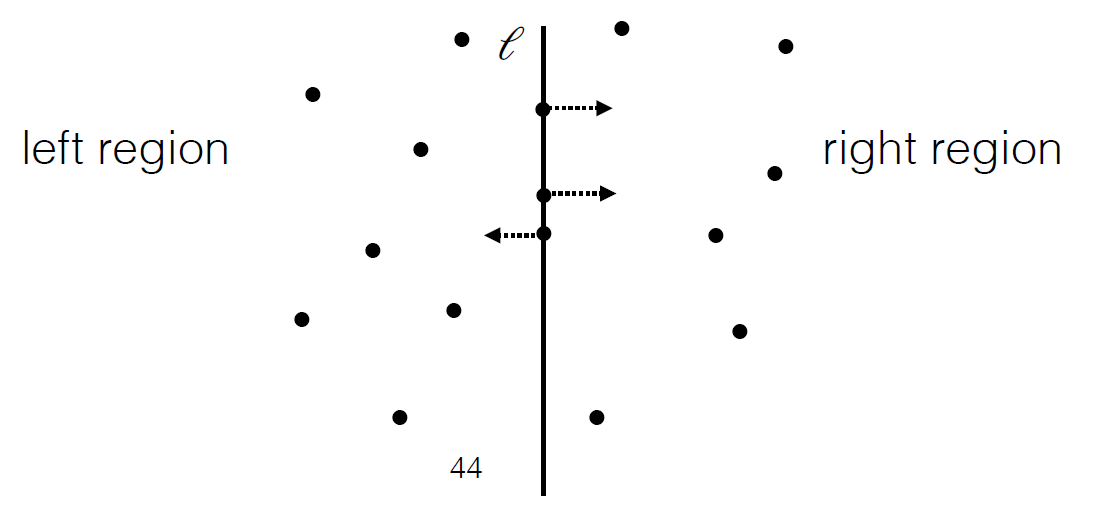
\includegraphics[width=0.55\textwidth]{closest-pair-division.png}
    \caption{平面分割示意图}
    \label{fig:closest-pair-division}
\end{figure}
\subsubsection{Phase III：递归求解}

\begin{method}[递归求左右最近距离]
分别递归求出左区域和右区域的最近点对距离，记为 $d_L$ 和 $d_R$。令
\[
d = \min(d_L, d_R).
\]
\end{method}

\begin{remark}
此时全局最近点对可能出现在：
\begin{enumerate}
    \item 左区域内部（距离为 $d_L$）；
    \item 右区域内部（距离为 $d_R$）；
    \item \textbf{跨区域}：一个点在左区域，一个点在右区域。
\end{enumerate}
前两种情形已在递归中求出，关键在于如何高效检验第三种情形。
\end{remark}

\begin{figure}[htbp]
    \centering
    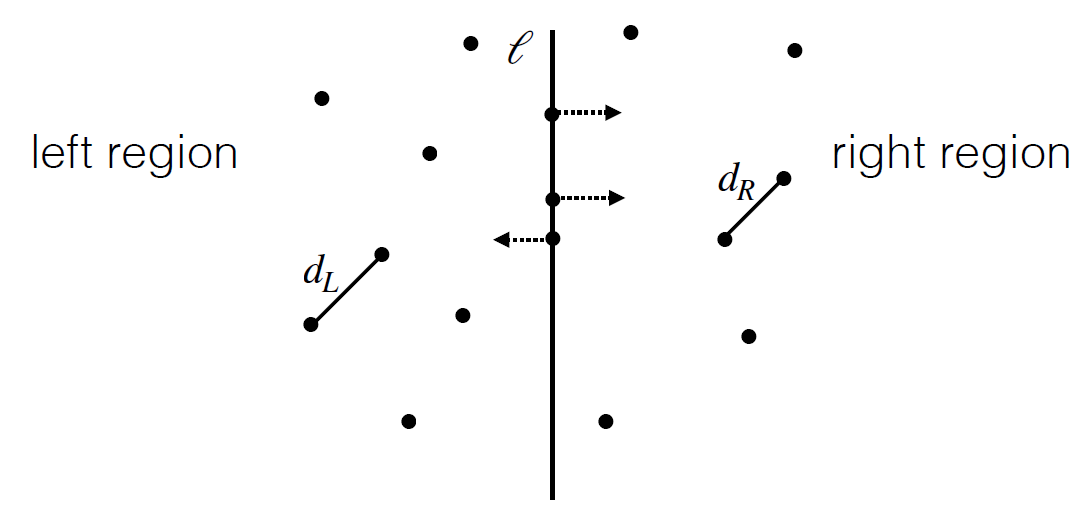
\includegraphics[width=0.6\textwidth]{closest-pair-recursion.png}
    \caption{递归求解示意图}
    \label{fig:closest-pair-recursion}
\end{figure}

\subsubsection{Phase IV：跨区最近点对检验}

\begin{method}[条带筛选]
若存在跨区最近点对，则两点的 $x$ 坐标之差必不超过 $d$。因此只需考虑以分割线 $\ell$ 为中心、宽度为 $2d$ 的\textbf{垂直条带}（vertical strip）内的点。条带外的点与另一侧点的距离必大于 $d$，不可能是全局最近点对。
\end{method}

\begin{figure}[htbp]
    \centering
    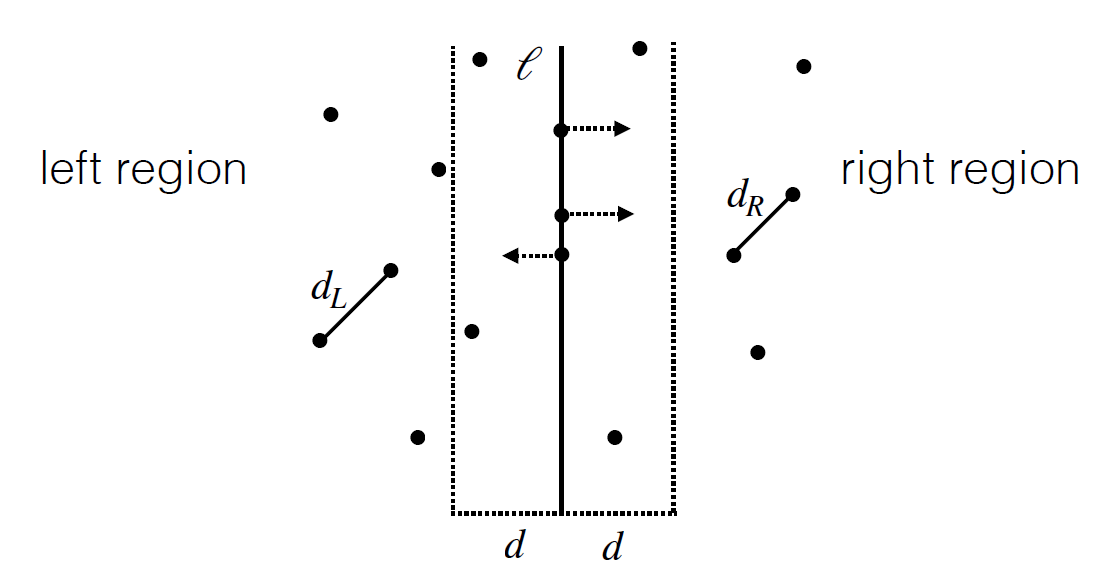
\includegraphics[width=0.6\textwidth]{closest-pair-strip.png}
    \caption{垂直条带示意图}
    \label{fig:closest-pair-strip}
\end{figure}

\begin{claim}[跨区比较的上界]
在 Phase IV 中，利用按 $y$ 坐标排序的序列，对垂直条带内的每个点 $p$（按 $y$ 从小到大处理），只需计算 $p$ 与位于其上方、高度为 $d$、宽度为 $2d$ 的矩形区域内的\textbf{最多 4 个点}的距离即可。
\end{claim}

\begin{proof}[Claim 证明]
将垂直条带内位于点 $p$ 上方、高度为 $d$ 的矩形区域（宽 $2d$、高 $d$）划分为 $8$ 个大小为 $(d/2)\times(d/2)$ 的小方块：左右各 $4$ 个（每侧 $2$ 列 $\times$ $2$ 行），如下图所示。

\begin{center}
\begin{tabular}{|c|c|c|c|}
\hline
\multicolumn{2}{|c|}{左区域} & \multicolumn{2}{c|}{右区域} \\
\hline
$d/2$ & $d/2$ & $d/2$ & $d/2$ \\
\hline
& & $\bullet$ & \\
\hline
& & $\bullet$ & \\
\hline
\multicolumn{2}{c}{$p$} & & \\
\hline
\end{tabular}
\end{center}

\textbf{关键观察}：每个 $(d/2)\times(d/2)$ 小方块的对角线长为
\[
\sqrt{(d/2)^2+(d/2)^2} = \frac{d}{\sqrt{2}} < d.
\]
因此：
\begin{itemize}
    \item 若某小方块内有 $2$ 个同属于左区域的点，则它们的距离 $<d\le d_L$，与 $d_L$ 是左区域最近距离矛盾；
    \item 同理，每个小方块内也至多含 $1$ 个右区域的点。
\end{itemize}

在检验跨区最近点对时，点 $p$ 只需与\textbf{另一侧}区域中的点比较（同一侧的点对已在递归中处理完毕）。不妨设 $p$ 位于左区域，则只需考虑右区域中位于 $p$ 上方、高度 $d$ 范围内的点。右区域在该范围内恰好占据 $4$ 个小方块（$2$ 列 $\times$ $2$ 行），每个小方块至多 $1$ 个点，故至多需要计算 \textbf{4 个距离}。

对于按 $y$ 坐标排序后的序列，处理点 $p$ 时只需检查其后（$y$ 坐标更大）的连续若干点，直到 $y$ 差超过 $d$ 即可停止。在此范围内，另一侧最多 $4$ 个点需要比较。
\end{proof}

\begin{figure}[htbp]
    \centering
    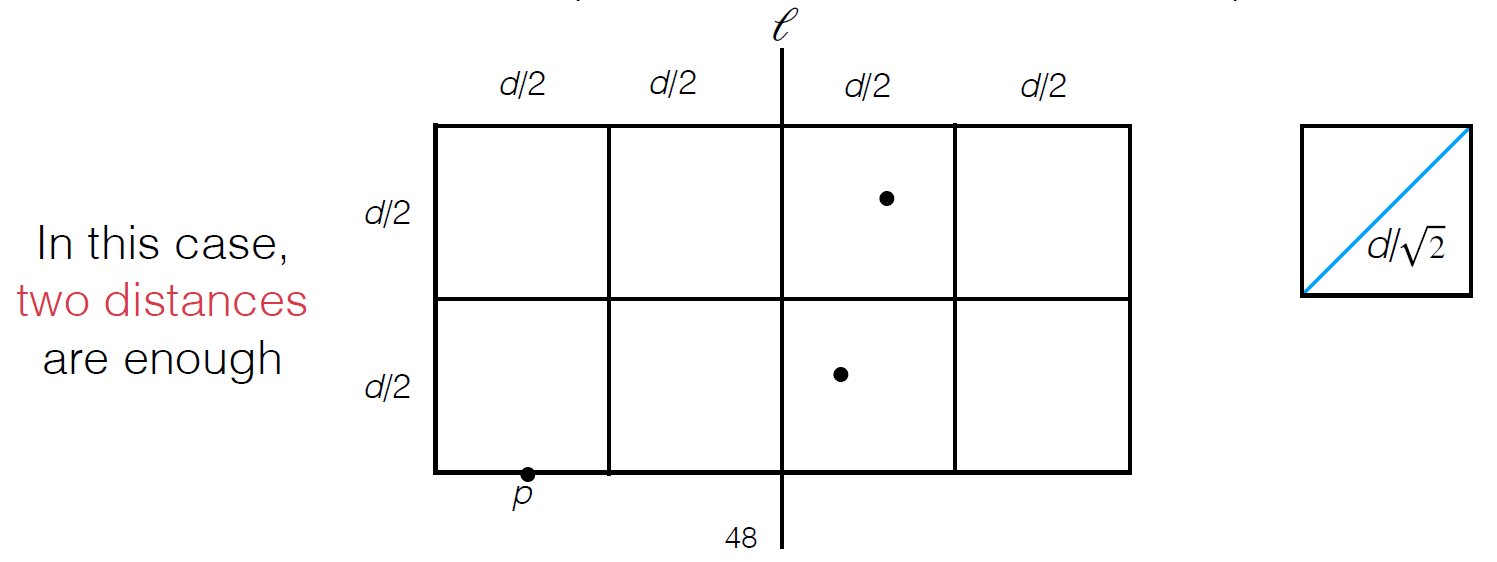
\includegraphics[width=0.7\textwidth]{closest-pair-blocks.png}
    \caption{小方块划分示意图}
    \label{fig:closest-pair-blocks}
\end{figure}

\begin{property}[Phase IV 的线性复杂度]
设条带内共有 $m$ 个点。由于每个点只需与后面最多 $4$ 个点比较，Phase IV 的距离计算次数为 $O(m)$。又因为条带内的点是从全局按 $y$ 排序序列中筛选得到的，整个筛选与比较过程可在 $O(n)$ 时间内完成。
\end{property}

%====================================================
\subsection{复杂度分析}
%====================================================

\begin{theorem}[最近点对分治算法复杂度]
设 $f(n)$ 为上述快速算法在 Phase II--IV 中所需的距离计算次数（或总操作次数），则 $f$ 满足分治递推关系：
\[
f(n) = 2f(n/2) + 4n,\qquad n\ \text{even},
\]
其中 $2f(n/2)$ 来自左右两区域的递归求解，$4n$ 来自 Phase IV 中每个点至多 $4$ 次跨区距离计算。
\end{theorem}

\begin{proof}[复杂度求解]
由主定理（定理 \ref{thm:master}），$a=2,b=2,d=1$。因 $a=b^d$（$2=2^1$），属于临界情形，故
\[
f(n) = O(n^d\log n) = O(n\log n).
\]

Phase I 的两次归并排序也各需 $O(n\log n)$。因此整个算法的时间复杂度为 $O(n\log n)$。
\end{proof}

%====================================================
\section*{课程总结（Recap）}
\addcontentsline{toc}{section}{课程总结}
%====================================================

本章（Lecture 45--46）涵盖以下核心内容：

\begin{itemize}
    \item \textbf{非齐次线性递推的解结构}（定理 \ref{thm:nonhom-structure}）：通解 = 特解 + 关联齐次通解。
    \item \textbf{待定系数法}（定理 \ref{thm:undet-coeff}）：当 $f(n)=P(n)\cdot s^n$ 时，根据 $s$ 是否为特征根及其重数选择特解形式。
    \item \textbf{分治递推关系}：标准形式 $f(n)=a\,f(n/b)+g(n)$，来源于二分搜索、Maxmin、归并排序、Karatsuba 乘法、Strassen 矩阵乘法等。
    \item \textbf{迭代展开法}：逐层展开递推式，将复杂度表示为 $a^k f(1)+\sum a^i g(n/b^i)$。
    \item \textbf{常数附加项的精确解}（定理 \ref{thm:dac-constant}）：$f(n)=C_1 n^{\log_b a}+C_2$（当 $n=b^k$ 且 $a>1$）。
    \item \textbf{主定理}（定理 \ref{thm:master}）：
    \[
    f(n)=
    \begin{cases}
    O(n^d), & a<b^d,\\[0.3em]
    O(n^d\log n), & a=b^d,\\[0.3em]
    O(n^{\log_b a}), & a>b^d.
    \end{cases}
    \]
    \item \textbf{最近点对问题}：分治四阶段算法，利用条带筛选与 $8$ 小方块论证将跨区比较降为每个点至多 $4$ 次，总复杂度 $O(n\log n)$。
\end{itemize}

%====================================================
\section*{作业}
\addcontentsline{toc}{section}{作业}
%====================================================

\begin{enumerate}
    \item 教材第 8.2 节：第 552 页，练习 30。\\
    \textbf{要求}：利用非齐次线性递推关系的两个定理（解结构定理 + 待定系数法）求解递推关系
    \[
    a_n = a_{n-1} + n^3,\qquad a_0 = 0.
    \]

    \item 教材第 8.3 节：第 562 页，练习 22；第 563 页，练习 36、37。
\end{enumerate}

\textbf{交作业时间}：奇数周周一上课前（两周交一次）。\\
\textbf{交作业方式}（二选一）：通过课程网站 \url{https://mooc.ucas.edu.cn/portal} 提交，或上课现场提交。\\
\textbf{答疑}：助教崔乐天、刘易铖。

\textbf{下次课程}：生成函数（Generating Functions）与广义容斥原理（Generalized Inclusion-Exclusion Principle）。

%====================================================
\section{生成函数（Generating Functions）}
%====================================================

\subsection{生成函数的定义与基本形式（Definition and Basic Forms）}

\begin{definition}[生成函数]
设 $\{a_n\}_{n=0}^{\infty}$ 是一个实数（或复数）序列，其\textbf{生成函数}（generating function）定义为形式幂级数
\[
G(x) = \sum_{k=0}^{\infty} a_k x^k = a_0 + a_1 x + a_2 x^2 + \cdots.
\]
若序列有限，即仅含 $a_0,a_1,\dots,a_n$，则其生成函数退化为 $n$ 次多项式
\[
G(x) = \sum_{k=0}^{n} a_k x^k.
\]
\end{definition}

\begin{remark}
生成函数的核心思想是将离散序列 ``编码'' 为幂级数的系数，从而将组合计数与递推问题转化为代数运算。形式幂级数（formal power series）的运算不依赖于收敛性，仅按系数的代数规则进行。
\end{remark}

\begin{example}[基本生成函数]
\begin{itemize}
    \item 常数序列 $\{1,1,1,\dots\}$ 的生成函数为
    \[
    \sum_{k=0}^{\infty} x^k = \frac{1}{1-x},
    \]
    后者称为该级数的\textbf{闭形式}（closed form）。
    \item 序列 $\{k+1\}_{k=0}^{\infty}$ 的生成函数为 $\displaystyle\sum_{k=0}^{\infty}(k+1)x^k$。
    \item 序列 $\{2^k\}_{k=0}^{\infty}$ 的生成函数为 $\displaystyle\sum_{k=0}^{\infty}2^k x^k = \frac{1}{1-2x}$。
    \item 有限序列 $\{1,1,1,1\}$（长度 $4$）的生成函数为
    \[
    \sum_{k=0}^{3} x^k = \frac{x^4-1}{x-1}.
    \]
    \item 对正整数 $m$，二项式系数序列 $\{\binom{m}{0},\binom{m}{1},\dots,\binom{m}{m}\}$ 的生成函数为
    \[
    \sum_{k=0}^{m}\binom{m}{k}x^k = (1+x)^m.
    \]
\end{itemize}
\end{example}

\begin{remark}
生成函数的思想最早由法国数学家 Abraham de Moivre（1667--1754）于 1730 年引入，用于系统地求解递推问题。
\end{remark}

%====================================================
\subsection{用生成函数计数（Counting by Generating Functions）}
%====================================================

生成函数将组合计数问题转化为幂级数的乘法：若对象 $A$ 的选取方式生成函数为 $F(x)$，对象 $B$ 的选取方式生成函数为 $H(x)$，则同时独立选取 $A$ 与 $B$ 的方式生成函数为 $F(x)\cdot H(x)$，其中乘积项 $x^n$ 的系数即为总规模为 $n$ 的方案数。

\begin{example}[凑零钱问题]\label{ex:change-making}
问：使用 $1$ 元与 $2$ 元人民币凑出 $n$ 元零钱，共有多少种方法？

\textbf{建模}：
\begin{itemize}
    \item $1$ 元面值可重复使用 $0,1,2,\dots$ 张，对应生成函数
    \[
    1+x+x^2+\cdots = \frac{1}{1-x}.
    \]
    \item $2$ 元面值可重复使用 $0,1,2,\dots$ 张，对应生成函数
    \[
    1+x^2+x^4+\cdots = \frac{1}{1-x^2}.
    \]
\end{itemize}

\textbf{总生成函数}：
\[
G(x) = \frac{1}{1-x}\cdot\frac{1}{1-x^2} = \frac{1}{(1-x)^2(1+x)}.
\]

\textbf{部分分式分解}：
\[
\frac{1}{(1-x)^2(1+x)} = \frac{1}{4}\cdot\frac{3-x}{(1-x)^2} + \frac{1}{4}\cdot\frac{1}{1+x}.
\]

\textbf{级数展开}：
利用 $\displaystyle\frac{1}{(1-x)^2}=\sum_{n=0}^{\infty}(n+1)x^n$ 与 $\displaystyle\frac{1}{1+x}=\sum_{n=0}^{\infty}(-1)^n x^n$，有
\begin{align*}
\frac{3-x}{(1-x)^2} &= (3-x)\sum_{n=0}^{\infty}(n+1)x^n \\
&= 3\sum_{n=0}^{\infty}(n+1)x^n - \sum_{n=0}^{\infty}(n+1)x^{n+1} \\
&= \sum_{n=0}^{\infty}3(n+1)x^n - \sum_{n=1}^{\infty}n x^n \\
&= 3 + \sum_{n=1}^{\infty}\bigl[3(n+1)-n\bigr]x^n \\
&= \sum_{n=0}^{\infty}(2n+3)x^n.
\end{align*}

因此
\begin{align*}
G(x) &= \frac{1}{4}\sum_{n=0}^{\infty}(2n+3)x^n + \frac{1}{4}\sum_{n=0}^{\infty}(-1)^n x^n \\
&= \frac{1}{4}\sum_{n=0}^{\infty}\bigl[2n+3+(-1)^n\bigr]x^n.
\end{align*}

\textbf{结论}：凑 $n$ 元零钱的方法数为
\[
\boxed{[x^n]G(x) = \frac{2n+3+(-1)^n}{4}}.
\]
\end{example}

\begin{example}[分配有限相同物品]\label{ex:cookies}
将 $8$ 块相同的饼干分给 $3$ 个不同的孩子，要求每个孩子至少得到 $2$ 块、至多得到 $4$ 块，问有多少种分配方法？

\textbf{建模}：
每个孩子可能得到 $2,3,4$ 块，对应生成函数为 $x^2+x^3+x^4$。三个孩子的总生成函数为
\[
G(x) = (x^2+x^3+x^4)^3.
\]

\textbf{求系数}：
提取 $x^8$ 的系数。先提取公因子：
\[
(x^2+x^3+x^4)^3 = x^6(1+x+x^2)^3,
\]
故需求 $(1+x+x^2)^3$ 中 $x^2$ 的系数。直接展开：
\[
(1+x+x^2)^3 = 1+3x+6x^2+7x^3+6x^4+3x^5+x^6,
\]
因此 $[x^2](1+x+x^2)^3 = 6$，进而 $[x^8]G(x)=6$。

\textbf{枚举验证}：满足条件的非负整数解 $(c_1,c_2,c_3)$（和为 $8$，每个分量在 $[2,4]$ 内）恰有
\[
(2,2,4),\ (2,4,2),\ (4,2,2),\ (2,3,3),\ (3,2,3),\ (3,3,2)
\]
共 $6$ 组，与生成函数结果一致。
\end{example}

%====================================================
\subsection{用生成函数求解递推关系（Solving Recurrence Relations by Generating Functions）}
%====================================================

对于常系数线性递推关系，生成函数可将递推式转化为关于 $G(x)$ 的代数方程，求解后再展开为幂级数即可得到通项公式。

\begin{example}[斐波那契数列的生成函数解法]\label{ex:gf-fibonacci}
求解递推关系
\[
F_n = F_{n-1}+F_{n-2},\qquad F_0=0,\ F_1=1.
\]

\textbf{第一步：建立生成函数方程。}

设 $\displaystyle G(x)=\sum_{n=0}^{\infty}F_n x^n$。利用递推式对 $n\ge 2$ 成立：
\begin{align*}
G(x) &= F_0+F_1x+\sum_{n=2}^{\infty}F_n x^n \\
&= x + \sum_{n=2}^{\infty}(F_{n-1}+F_{n-2})x^n \\
&= x + x\sum_{n=2}^{\infty}F_{n-1}x^{n-1} + x^2\sum_{n=2}^{\infty}F_{n-2}x^{n-2} \\
&= x + x\sum_{m=1}^{\infty}F_m x^m + x^2\sum_{k=0}^{\infty}F_k x^k \qquad(m=n-1,\ k=n-2)\\
&= x + x\bigl(G(x)-F_0\bigr) + x^2 G(x) \\
&= x + xG(x) + x^2G(x).
\end{align*}

\textbf{第二步：解代数方程。}

整理得
\[
G(x) = \frac{x}{1-x-x^2}.
\]

\textbf{第三步：因式分解与部分分式。}

分母的根满足 $x^2+x-1=0$，即 $x=\frac{-1\pm\sqrt{5}}{2}$。记
\[
\phi=\frac{1+\sqrt{5}}{2},\qquad \hat{\phi}=\frac{1-\sqrt{5}}{2}.
\]
注意到 $\phi+\hat{\phi}=1$，$\phi\hat{\phi}=-1$，因此
\[
1-x-x^2 = -(x^2+x-1) = -(x+\phi)(x+\hat{\phi}).
\]
于是
\[
G(x) = \frac{-x}{(x+\phi)(x+\hat{\phi})}
= \frac{x}{\sqrt{5}}\left(\frac{1}{x+\phi}-\frac{1}{x+\hat{\phi}}\right),
\]
其中利用了 $\phi-\hat{\phi}=\sqrt{5}$。

\textbf{第四步：展开为幂级数。}

将上式进一步改写为可直接展开的几何级数形式。通过通分可验证恒等式
\[
\frac{x}{1-x-x^2} = \frac{x}{\sqrt{5}}\left(\frac{\phi}{1-\phi x} - \frac{\hat{\phi}}{1-\hat{\phi} x}\right).
\]
将两项分别展开（形式幂级数意义上）：
\[
\frac{\phi}{1-\phi x} = \phi\sum_{n=0}^{\infty}(\phi x)^n = \sum_{n=0}^{\infty}\phi^{n+1}x^n,
\]
\[
\frac{\hat{\phi}}{1-\hat{\phi} x} = \hat{\phi}\sum_{n=0}^{\infty}(\hat{\phi} x)^n = \sum_{n=0}^{\infty}\hat{\phi}^{n+1}x^n.
\]

\textbf{第五步：提取系数。}

代入得
\begin{align*}
G(x) &= \frac{x}{\sqrt{5}}\left[\sum_{n=0}^{\infty}\phi^{n+1}x^n - \sum_{n=0}^{\infty}\hat{\phi}^{n+1}x^n\right] \\
&= \frac{1}{\sqrt{5}}\sum_{n=0}^{\infty}\bigl(\phi^{n+1}-\hat{\phi}^{n+1}\bigr)x^{n+1} \\
&= \frac{1}{\sqrt{5}}\sum_{n=1}^{\infty}\bigl(\phi^{n}-\hat{\phi}^{n}\bigr)x^{n}.
\end{align*}
由于 $F_0=0$，上式对 $n=0$ 亦成立（此时 $\phi^0-\hat{\phi}^0=0$）。对比 $G(x)=\sum_{n=0}^{\infty}F_n x^n$，得到
\[
\boxed{F_n = \frac{1}{\sqrt{5}}\left[\left(\frac{1+\sqrt{5}}{2}\right)^n - \left(\frac{1-\sqrt{5}}{2}\right)^n\right]},\qquad n\ge 0.
\]
这正是斐波那契数列的\textbf{比内公式}（Binet's formula）。
\end{example}

\begin{remark}
生成函数法求解递推关系的关键步骤可概括为：
\begin{enumerate}
    \item 设 $G(x)=\sum a_n x^n$，利用递推关系将级数重组为关于 $G(x)$ 的方程；
    \item 解代数方程得到 $G(x)$ 的闭形式（通常为有理函数）；
    \item 对有理函数进行部分分式分解；
    \item 将各简单分式展开为已知幂级数，合并后提取 $x^n$ 系数。
\end{enumerate}
\end{remark}

%====================================================
\subsection{形式幂级数的基本运算与闭形式（Basic Operations and Closed Forms）}
%====================================================

\begin{definition}[形式幂级数的运算]
设 $f(x)=\sum_{k=0}^{\infty}a_k x^k$，$g(x)=\sum_{k=0}^{\infty}b_k x^k$ 为两个形式幂级数，定义：
\begin{itemize}
    \item \textbf{加法}：$f(x)+g(x)=\sum_{k=0}^{\infty}(a_k+b_k)x^k$；
    \item \textbf{数乘}：$c\cdot f(x)=\sum_{k=0}^{\infty}(c a_k)x^k$；
    \item \textbf{乘法（柯西乘积 / 卷积）}：
    \[
    f(x)g(x)=\sum_{k=0}^{\infty}\left(\sum_{j=0}^{k}a_j b_{k-j}\right)x^k.
    \]
\end{itemize}
\end{definition}

\begin{theorem}[几何级数及其推广]
对任意非零常数 $a$，有形式幂级数恒等式
\[
\sum_{k=0}^{\infty}a^k x^k=\frac{1}{1-ax}.
\]
特别地，当 $a=1$ 时，$\displaystyle\sum_{k=0}^{\infty}x^k=\frac{1}{1-x}$。
\end{theorem}

\begin{example}[平方倒数生成函数]
由几何级数乘法规则（卷积），
\[
\frac{1}{(1-x)^2}=\left(\sum_{k=0}^{\infty}x^k\right)^2=\sum_{k=0}^{\infty}\left(\sum_{j=0}^{k}1\cdot 1\right)x^k=\sum_{k=0}^{\infty}(k+1)x^k.
\]
因此序列 $\{1,2,3,\dots\}$ 的生成函数为 $1/(1-x)^2$，而 $\{0,1,2,3,\dots\}$ 的生成函数为 $x/(1-x)^2$。
\end{example}

%====================================================
\subsection{扩展二项式定理（Extended Binomial Theorem）}
%====================================================

\begin{definition}[广义二项式系数]
设 $u\in\mathbb{R}$（或 $\mathbb{C}$），$k\in\mathbb{N}$。定义\textbf{广义二项式系数}（extended binomial coefficient）为
\[
\binom{u}{k}=
\begin{cases}
\dfrac{u(u-1)\cdots(u-k+1)}{k!}, & k>0,\\[0.8em]
1, & k=0.
\end{cases}
\]
\end{definition}

\begin{example}[广义二项式系数计算]
\begin{itemize}
    \item $\displaystyle\binom{-2}{3}=\frac{(-2)(-3)(-4)}{3!}=-4$；
    \item $\displaystyle\binom{1/2}{3}=\frac{(1/2)(-1/2)(-3/2)}{3!}=\frac{1}{16}$；
    \item 对正整数 $n$，有重要恒等式
    \[
    \binom{-n}{r}=\frac{(-n)(-n-1)\cdots(-n-r+1)}{r!}=(-1)^r\binom{n+r-1}{r}.
    \]
\end{itemize}
\end{example}

\begin{theorem}[扩展二项式定理]\label{thm:extended-binomial}
设 $u\in\mathbb{R}$，则形式幂级数意义下有
\[
(1+x)^u=\sum_{k=0}^{\infty}\binom{u}{k}x^k.
\]
作为解析函数，该展开在 $|x|<1$ 时收敛。
\end{theorem}

\begin{proof}[证明（Taylor 展开法）]
设 $f(x)=(1+x)^u$。逐次求导得
\[
f^{(k)}(x)=u(u-1)\cdots(u-k+1)(1+x)^{u-k},
\]
故 $f^{(k)}(0)=u(u-1)\cdots(u-k+1)$。代入 Taylor 展开式
\[
f(x)=\sum_{k=0}^{\infty}\frac{f^{(k)}(0)}{k!}x^k
=\sum_{k=0}^{\infty}\binom{u}{k}x^k.
\]
在 $|x|<1$ 时该级数收敛于 $(1+x)^u$。
\end{proof}

\begin{proof}[证明（微分方程法，形式幂级数视角）]
设 $g(x)=\sum_{k=0}^{\infty}\binom{u}{k}x^k$。逐项求导（形式导数）得
\[
g'(x)=\sum_{k=1}^{\infty}\binom{u}{k}k x^{k-1}
=\sum_{k=0}^{\infty}\binom{u}{k+1}(k+1)x^k.
\]
利用恒等式 $\displaystyle\binom{u}{k+1}(k+1)=u\binom{u}{k}$，有
\[
g'(x)=u\sum_{k=0}^{\infty}\binom{u}{k}x^k=u\cdot g(x).
\]
同时 $\displaystyle\frac{\mathrm{d}}{\mathrm{d}x}(1+x)^u=u(1+x)^{u-1}=\frac{u}{1+x}(1+x)^u$。构造函数 $h(x)=g(x)/(1+x)^u$，则
\[
h'(x)=\frac{g'(x)(1+x)^u-g(x)\cdot u(1+x)^{u-1}}{(1+x)^{2u}}
=\frac{u g(x)(1+x)^{u-1}-u g(x)(1+x)^{u-1}}{(1+x)^{2u}}=0.
\]
故 $h(x)$ 为常数。由 $h(0)=g(0)/1=1$，得 $h(x)\equiv 1$，即 $g(x)=(1+x)^u$。
\end{proof}

\begin{corollary}[负指数展开]
对正整数 $n$，有
\[
\frac{1}{(1+x)^n}=(1+x)^{-n}=\sum_{k=0}^{\infty}(-1)^k\binom{n+k-1}{k}x^k,
\]
\[
\frac{1}{(1-x)^n}=(1-x)^{-n}=\sum_{k=0}^{\infty}\binom{n+k-1}{k}x^k.
\]
\end{corollary}

\begin{proof}
由扩展二项式定理及 $\binom{-n}{k}=(-1)^k\binom{n+k-1}{k}$，分别代入 $u=-n$ 并以 $-x$ 替换 $x$ 即得。
\end{proof}

\begin{example}[重复组合计数]
从 $n$ 种不同物体中选取 $r$ 个，每种至少选一个，方案数等价于求
\[
(x+x^2+\cdots)^n=\frac{x^n}{(1-x)^n}
\]
中 $x^r$ 的系数。由负指数展开，
\[
\frac{x^n}{(1-x)^n}=x^n\sum_{k=0}^{\infty}\binom{n+k-1}{k}x^k
=\sum_{k=0}^{\infty}\binom{n+k-1}{n-1}x^{n+k}.
\]
令 $n+k=r$，即 $k=r-n$，得系数为 $\displaystyle\binom{r-1}{r-n}=\binom{r-1}{n-1}$，与重复组合公式一致。
\end{example}

%====================================================
\subsection{常用生成函数表（Table of Common Generating Functions）}
%====================================================

下表列出离散数学中常用的生成函数及其对应序列，便于快速查阅。

\begin{table}[htbp]
\centering
\caption{常用生成函数对照表}\label{tab:common-gf}
\begin{tabular}{|l|l|l|}
\hline
\textbf{序列 $\{a_n\}_{n=0}^{\infty}$} & \textbf{生成函数 $G(x)$} & \textbf{备注} \\
\hline
$1,1,1,\dots$ & $\displaystyle\frac{1}{1-x}$ & 几何级数 \\
\hline
$1,-1,1,-1,\dots$ & $\displaystyle\frac{1}{1+x}$ & 交错几何级数 \\
\hline
$1,a,a^2,\dots$ & $\displaystyle\frac{1}{1-ax}$ & 广义几何级数 \\
\hline
$1,2,3,4,\dots$ & $\displaystyle\frac{1}{(1-x)^2}$ & 自然数序列 \\
\hline
$0,1,2,3,\dots$ & $\displaystyle\frac{x}{(1-x)^2}$ & 移位自然数序列 \\
\hline
$\binom{m}{0},\binom{m}{1},\dots,\binom{m}{m}$ & $(1+x)^m$ & 二项式定理，$m\in\mathbb{N}$ \\
\hline
$\binom{n+k-1}{k}$（固定 $n$） & $\displaystyle\frac{1}{(1-x)^n}$ & 负二项展开 \\
\hline
$\binom{n}{0},2\binom{n}{1},2^2\binom{n}{2},\dots$ & $(1+2x)^n$ & 广义二项式 \\
\hline
$C_n=\frac{1}{n+1}\binom{2n}{n}$ & $\displaystyle\frac{1-\sqrt{1-4x}}{2x}$ & 卡特兰数 \\
\hline
$1,1,\frac{1}{2!},\frac{1}{3!},\dots$ & $e^x$ & 指数生成函数* \\
\hline
$0,1,\frac{1}{2},\frac{1}{3},\dots$ & $-\ln(1-x)$ & 对数级数 \\
\hline
\end{tabular}
\end{table}

\begin{remark}
表中带 * 号的 $e^x$ 属于\textbf{指数生成函数}（exponential generating function），其形式为 $\displaystyle\sum_{n=0}^{\infty}a_n\frac{x^n}{n!}$，常用于排列计数问题。本课程主要讨论普通生成函数（ordinary generating function）。
\end{remark}

%====================================================
\subsection{卡特兰数的生成函数解法（Catalan Numbers via Generating Functions）}
%====================================================

\begin{recall}[卡特兰数递推关系]
回顾括号化问题：$n+1$ 个数的乘积 $x_0x_1\cdots x_n$ 的括号化方式数 $C_n$ 满足
\[
C_0=1,\qquad C_n=\sum_{k=0}^{n-1}C_k C_{n-1-k}\quad(n\ge 1).
\]
\end{recall}

\begin{theorem}[卡特兰数闭公式]
卡特兰数的生成函数为
\[
G(x)=\sum_{n=0}^{\infty}C_n x^n=\frac{1-\sqrt{1-4x}}{2x},
\]
且其显式公式为
\[
\boxed{C_n=\frac{1}{n+1}\binom{2n}{n}\qquad(n\ge 0).}
\]
\end{theorem}

\begin{proof}[证明]
\textbf{第一步：建立生成函数方程。}

设 $\displaystyle G(x)=\sum_{n=0}^{\infty}C_n x^n$。由递推关系，对 $n\ge 1$：
\begin{align*}
G(x) &= C_0 + \sum_{n=1}^{\infty}C_n x^n \\
&= 1 + \sum_{n=1}^{\infty}\left(\sum_{k=0}^{n-1}C_k C_{n-1-k}\right)x^n.
\end{align*}
注意到内层求和正是序列 $\{C_n\}$ 与自身的卷积。具体地，
\[
\left(\sum_{k=0}^{\infty}C_k x^k\right)\left(\sum_{j=0}^{\infty}C_j x^j\right)
=\sum_{n=0}^{\infty}\left(\sum_{k=0}^{n}C_k C_{n-k}\right)x^n.
\]
对比可知 $\sum_{k=0}^{n-1}C_k C_{n-1-k}$ 是 $x^{n-1}$ 的系数，因此
\[
\sum_{n=1}^{\infty}\left(\sum_{k=0}^{n-1}C_k C_{n-1-k}\right)x^n
= x\sum_{n=1}^{\infty}\left(\sum_{k=0}^{n-1}C_k C_{n-1-k}\right)x^{n-1}
= x\cdot G(x)^2.
\]
于是得到\textbf{生成函数方程}：
\[
\boxed{G(x)=1+xG(x)^2.}
\]

\textbf{第二步：解代数方程。}

将上式视为关于 $G(x)$ 的二次方程：
\[
x\cdot G(x)^2 - G(x) + 1 = 0.
\]
由求根公式，
\[
G(x)=\frac{1\pm\sqrt{1-4x}}{2x}.
\]
需要确定符号。当 $x\to 0$ 时，$G(0)=C_0=1$。考察两支：
\begin{itemize}
    \item 取 $+$ 号：$\displaystyle\frac{1+\sqrt{1-4x}}{2x}\sim\frac{2}{2x}=\frac{1}{x}\to\infty$，与 $G(0)=1$ 矛盾；
    \item 取 $-$ 号：由 $\sqrt{1-4x}=1-2x-2x^2-\cdots$，有
    \[
    \frac{1-\sqrt{1-4x}}{2x}=\frac{2x+2x^2+\cdots}{2x}=1+x+\cdots\to 1.
    \]
\end{itemize}
故必须取\textbf{负号}：
\[
G(x)=\frac{1-\sqrt{1-4x}}{2x}.
\]

\textbf{第三步：展开为幂级数。}

利用扩展二项式定理展开 $\sqrt{1-4x}=(1-4x)^{1/2}$：
\begin{align*}
(1-4x)^{1/2} &= \sum_{n=0}^{\infty}\binom{1/2}{n}(-4x)^n \\
&= 1 + \sum_{n=1}^{\infty}\frac{(1/2)(-1/2)(-3/2)\cdots(3/2-n)}{n!}(-4)^n x^n.
\end{align*}
对 $n\ge 1$，计算系数：
\begin{align*}
\binom{1/2}{n}(-4)^n
&= \frac{(1/2)(-1/2)\cdots((3-2n)/2)}{n!}(-4)^n \\
&= \frac{(-1)^{n-1}(1\cdot 3\cdot 5\cdots(2n-3))}{2^n n!}(-4)^n \\
&= \frac{(-1)^{n-1}(-1)^n 4^n}{2^n n!}\cdot\frac{(2n-2)!}{2^{n-1}(n-1)!} \\
&= -\frac{2}{n}\binom{2n-2}{n-1}.
\end{align*}
（其中利用了双阶乘化简：$1\cdot 3\cdots(2n-3)=\dfrac{(2n-2)!}{2^{n-1}(n-1)!}$。）

因此
\[
(1-4x)^{1/2}=1-\sum_{n=1}^{\infty}\frac{2}{n}\binom{2n-2}{n-1}x^n.
\]
代入 $G(x)$：
\begin{align*}
G(x) &= \frac{1}{2x}\left(1-\left[1-\sum_{n=1}^{\infty}\frac{2}{n}\binom{2n-2}{n-1}x^n\right]\right) \\
&= \frac{1}{2x}\sum_{n=1}^{\infty}\frac{2}{n}\binom{2n-2}{n-1}x^n \\
&= \sum_{n=1}^{\infty}\frac{1}{n}\binom{2n-2}{n-1}x^{n-1}.
\end{align*}
令 $m=n-1$（即 $n=m+1$），则
\[
G(x)=\sum_{m=0}^{\infty}\frac{1}{m+1}\binom{2m}{m}x^m.
\]

\textbf{第四步：提取系数。}

对比 $G(x)=\sum_{m=0}^{\infty}C_m x^m$，即得
\[
C_m=\frac{1}{m+1}\binom{2m}{m},\qquad m\ge 0.
\]
证毕。
\end{proof}

\begin{remark}
卡特兰数的生成函数满足二次方程 $G=1+xG^2$，这是非线性递推关系难以用特征方程法求解、但生成函数法极为有效的典型例证。该方程的解 $\dfrac{1-\sqrt{1-4x}}{2x}$ 也是组合数学中最重要的代数生成函数之一。
\end{remark}

%====================================================
\section{广义容斥原理（Generalized Inclusion-Exclusion Principle）}
%====================================================

\subsection{从两个集合到多个集合（From Two Sets to Many）}

回顾两个集合的容斥原理：
\[
|A\cup B|=|A|+|B|-|A\cap B|.
\]
对于三个集合，有
\[
|A\cup B\cup C|=|A|+|B|+|C|-|A\cap B|-|B\cap C|-|A\cap C|+|A\cap B\cap C|.
\]

其组合意义在于：直接将各集合大小相加会导致交集部分被重复计数，因此需要交替地减去多重重叠、加上更高重重叠，直至每个元素恰好被计数一次。

%====================================================
\subsection{广义容斥原理的表述（General Formulation）}
%====================================================

\begin{theorem}[广义容斥原理]
\label{thm:generalized-iep}
设 $A_1,A_2,\dots,A_n$ 为有限集合，则
\[
|A_1\cup A_2\cup\cdots\cup A_n|
=\sum_{i}|A_i|
-\sum_{1\le i<j\le n}|A_i\cap A_j|
+\sum_{1\le i<j<k\le n}|A_i\cap A_j\cap A_k|
-\cdots
+(-1)^{n+1}|A_1\cap A_2\cap\cdots\cap A_n|.
\]
\end{theorem}

\begin{proof}[证明]
设 $a\in A_1\cup\cdots\cup A_n$ 为并集中任意一个元素。令 $k$（$1\le k\le n$）为 $a$ 恰好属于的集合个数，不妨设这些集合为 $A_{i_1},\dots,A_{i_k}$。

在定理右端，$a$ 被计数的次数如下：
\begin{itemize}
    \item 在单集合项 $\sum|A_i|$ 中，被计数 $\binom{k}{1}$ 次；
    \item 在两两交集项 $-\sum|A_i\cap A_j|$ 中，被计数 $-\binom{k}{2}$ 次；
    \item 在三三交集项 $+\sum|A_i\cap A_j\cap A_k|$ 中，被计数 $\binom{k}{3}$ 次；
    \item $\cdots$
    \item 在 $k$ 重交集项中，被计数 $(-1)^{k+1}\binom{k}{k}$ 次；
    \item 在超过 $k$ 重的交集中，$a$ 不被计数（因 $a$ 不属于那些集合）。
\end{itemize}

因此 $a$ 被计数的总次数为
\[
S=\binom{k}{1}-\binom{k}{2}+\binom{k}{3}-\cdots+(-1)^{k+1}\binom{k}{k}.
\]
由二项式定理，
\[
(1-1)^k=\sum_{j=0}^{k}(-1)^j\binom{k}{j}=1-S=0,
\]
故 $S=1$。即并集中每个元素在右端恰好被计数一次，等式成立。
\end{proof}

%====================================================
\subsection{容斥原理的补集形式（Alternative Form）}
%====================================================

在计数问题中，更常见的需求是计算\textbf{不具有任何给定性质}的元素个数。设 $U$ 为有限全集，$|U|=N$，$A_i\subseteq U$ 为具有性质 $P_i$ 的元素集合。

\begin{definition}[性质计数记号]
记 $N(P_{i_1}P_{i_2}\cdots P_{i_k})=|A_{i_1}\cap A_{i_2}\cap\cdots\cap A_{i_k}|$，表示同时具有性质 $P_{i_1},\dots,P_{i_k}$ 的元素个数；记 $N(P_{i_1}'P_{i_2}'\cdots P_{i_k}')$ 为\textbf{不具有}这些性质的元素个数。
\end{definition}

\begin{theorem}[容斥原理的补集形式]\label{thm:complement-iep}
在上述记号下，全集中不具有任何性质 $P_1,\dots,P_n$ 的元素个数为
\[
N(P_1'P_2'\cdots P_n')
= N
-\sum_{1\le i\le n}N(P_i)
+\sum_{1\le i<j\le n}N(P_iP_j)
-\sum_{1\le i<j<k\le n}N(P_iP_jP_k)
+\cdots
+(-1)^n N(P_1P_2\cdots P_n).
\]
\end{theorem}

\begin{proof}
注意到 $N(P_1'\cdots P_n')=|U|-|A_1\cup\cdots\cup A_n|$，将定理 \ref{thm:generalized-iep} 代入并整理即得。
\end{proof}

\begin{remark}
该形式在``筛法''类问题中尤为实用：全集 $U$ 代表所有候选对象，性质 $P_i$ 代表``被第 $i$ 个条件排除''，则补集形式直接给出``通过所有筛选''的对象数量。
\end{remark}

%====================================================
\subsection{应用：埃拉托斯特尼筛法（Sieves of Eratosthenes）}
%====================================================

\begin{example}[计算不超过 $100$ 的素数个数]\label{ex:sieve-100}
求不超过 $100$ 的正整数中素数的个数。

\textbf{分析}：由试除法与算术基本定理，$1<x\le 100$ 的整数不是素数，当且仅当它能被某个不超过 $\sqrt{100}=10$ 的素数整除。不超过 $10$ 的素数恰有 $4$ 个：$2,3,5,7$。

设全集 $U=\{1,2,\dots,100\}$（$N=100$），定义性质：
\begin{itemize}
    \item $P_1$：被 $2$ 整除；
    \item $P_2$：被 $3$ 整除；
    \item $P_3$：被 $5$ 整除；
    \item $P_4$：被 $7$ 整除。
\end{itemize}

\textbf{计算各交集大小}（利用 $\lfloor 100/d\rfloor$ 计算被 $d$ 整除的数的个数）：

单个性质：
\begin{align*}
N(P_1)&=\lfloor 100/2\rfloor=50, & N(P_2)&=\lfloor 100/3\rfloor=33,\\
N(P_3)&=\lfloor 100/5\rfloor=20, & N(P_4)&=\lfloor 100/7\rfloor=14.
\end{align*}

两两性质（最小公倍数即乘积，因均为素数）：
\begin{align*}
N(P_1P_2)&=\lfloor 100/6\rfloor=16, & N(P_1P_3)&=\lfloor 100/10\rfloor=10,\\
N(P_1P_4)&=\lfloor 100/14\rfloor=7, & N(P_2P_3)&=\lfloor 100/15\rfloor=6,\\
N(P_2P_4)&=\lfloor 100/21\rfloor=4, & N(P_3P_4)&=\lfloor 100/35\rfloor=2.
\end{align*}

三三性质：
\begin{align*}
N(P_1P_2P_3)&=\lfloor 100/30\rfloor=3, & N(P_1P_2P_4)&=\lfloor 100/42\rfloor=2,\\
N(P_1P_3P_4)&=\lfloor 100/70\rfloor=1, & N(P_2P_3P_4)&=\lfloor 100/105\rfloor=0.
\end{align*}

四四性质：
\[
N(P_1P_2P_3P_4)=\lfloor 100/210\rfloor=0.
\]

\textbf{应用容斥原理（补集形式）}：

被 $2,3,5,7$ 中至少一个整除的整数个数为
\begin{align*}
|A_1\cup A_2\cup A_3\cup A_4|
&=(50+33+20+14)\\
&\quad-(16+10+7+6+4+2)\\
&\quad+(3+2+1+0)\\
&\quad-0\\
&=117-45+6\\
&=78.
\end{align*}

\textbf{求素数个数}：

上述 $78$ 个数包含所有能被 $2,3,5,7$ 整除的数，其中包括素数 $2,3,5,7$ 本身（它们被错误地计为``合数''）。因此：
\begin{itemize}
    \item 真正的合数个数：$78-4=74$；
    \item 加上 $1$ 既非素数也非合数，故 $1$ 到 $100$ 中非素数共 $74+1=75$；
    \item 素数个数：$100-75=25$。
\end{itemize}

\textbf{结论}：不超过 $100$ 的素数共有 $\boxed{25}$ 个。
\end{example}

\begin{remark}
埃拉托斯特尼筛法的本质正是容斥原理的直观实现：要找出所有素数，只需从自然数中``筛去''所有小素数的倍数。容斥原理给出了被筛去数量的精确解析表达式，从而可计算任意范围内素数的个数（在只考虑有限个小素数因子时）。
\end{remark}

%====================================================
\section{广义容斥原理的应用（Applications of Generalized Inclusion-Exclusion Principle）}
%====================================================

\subsection{埃拉托斯特尼筛法的完整计算（Completed Sieve of Eratosthenes）}

\begin{example}
在例 \ref{ex:sieve-100} 中，若将全集严格取为 $U=\{2,3,\dots,100\}$（即排除 $1$，因 $1$ 既非素数也非合数），则 $N=99$。利用已算得的各交集大小，由补集形式（定理 \ref{thm:complement-iep}）：

\begin{align*}
N(P_1'P_2'P_3'P_4')
&= 99 - (50+33+20+14)\\
&\quad +(16+10+7+6+4+2)\\
&\quad -(3+2+1+0)\\
&\quad +0\\
&= 99 - 117 + 45 - 6\\
&= \boxed{21}.
\end{align*}

这 $21$ 个数恰为 $2$ 到 $100$ 之间不被 $2,3,5,7$ 任何一个小素数整除的数，它们正是所有大于 $7$ 且不超过 $100$ 的素数。再加上 $2,3,5,7$ 这四个小素数本身，得到不超过 $100$ 的素数共有
\[
21+4=\boxed{25}
\]
个。这与素数计数函数 $\pi(100)=25$ 完全一致。
\end{example}

%====================================================
\subsection{满射函数的数量（Number of Onto Functions）}
%====================================================

\begin{problem}
设 $A=\{a_1,\dots,a_m\}$，$B=\{b_1,\dots,b_n\}$，其中 $m\ge n\ge 1$。问：从 $A$ 到 $B$ 的\textbf{满射函数}（onto functions / surjective functions）有多少个？
\end{problem}

\begin{theorem}[满射函数计数公式]\label{thm:onto-functions}
从 $m$ 元集到 $n$ 元集的满射函数个数为
\[
\boxed{\sum_{j=0}^{n-1}(-1)^j\binom{n}{j}(n-j)^m
= n^m - \binom{n}{1}(n-1)^m + \binom{n}{2}(n-2)^m - \cdots + (-1)^{n-1}\binom{n}{n-1}\cdot 1^m.}
\]
\end{theorem}

\begin{proof}
设全集 $U$ 为所有函数 $f:A\to B$，则 $N=|U|=n^m$（每个 $a_i$ 独立选择 $n$ 个像之一）。

定义性质 $P_i$（$1\le i\le n$）：$b_i$ 不在 $f$ 的值域中，即 $f$ 遗漏了 $b_i$。则满射函数恰好是\textbf{不具有}任何性质 $P_1,\dots,P_n$ 的函数，其个数为 $N(P_1'P_2'\cdots P_n')$。

对任意 $k$ 个不同下标 $i_1,\dots,i_k$，同时满足 $P_{i_1},\dots,P_{i_k}$ 的函数意味着值域避开 $b_{i_1},\dots,b_{i_k}$，每个 $a_j$ 只能从剩下的 $n-k$ 个元素中选像，故
\[
N(P_{i_1}P_{i_2}\cdots P_{i_k})=(n-k)^m.
\]

代入广义容斥原理的补集形式（定理 \ref{thm:complement-iep}）：
\begin{align*}
N(P_1'\cdots P_n')
&= N - \sum_{i}N(P_i) + \sum_{i<j}N(P_iP_j) - \cdots + (-1)^n N(P_1\cdots P_n)\\
&= n^m - \binom{n}{1}(n-1)^m + \binom{n}{2}(n-2)^m - \cdots + (-1)^{n-1}\binom{n}{n-1}\cdot 1^m + (-1)^n\binom{n}{n}\cdot 0^m.
\end{align*}
由于 $m\ge 1$，有 $0^m=0$，故最后一项消失，求和可止于 $j=n-1$，即得所求公式。
\end{proof}

\begin{example}[作业分配问题]
将 $5$ 份不同的作业分配给 $4$ 名雇员，要求每名雇员至少得到一份，共有多少种分配方式？

这是从 $5$ 元集到 $4$ 元集的满射函数计数（$m=5,n=4$）。代入定理 \ref{thm:onto-functions}：
\begin{align*}
&\quad 4^5 - \binom{4}{1}3^5 + \binom{4}{2}2^5 - \binom{4}{3}1^5\\
&= 1024 - 4\cdot 243 + 6\cdot 32 - 4\cdot 1\\
&= 1024 - 972 + 192 - 4\\
&= \boxed{240}.
\end{align*}
\end{example}

%====================================================
\subsection{错位排列（Derangements）}
%====================================================

\begin{definition}[错位排列]
$n$ 个不同对象的一个\textbf{错位排列}（derangement）是指一个排列，其中\textbf{没有任何对象保持其原始位置}（即没有不动点）。记 $D_n$ 为 $n$ 个对象的错位排列数。

例如：$D_1=0$（单个元素无法错位）；$D_2=1$（仅交换）；$D_3=2$（$(1,2,3)\to(2,3,1)$ 与 $(1,2,3)\to(3,1,2)$）。
\end{definition}

\begin{theorem}[错位排列数公式]\label{thm:derangement}
$n$ 个对象的错位排列数为
\[
\boxed{D_n = n!\left[1-\frac{1}{1!}+\frac{1}{2!}-\frac{1}{3!}+\cdots+(-1)^n\frac{1}{n!}\right]
= \sum_{i=0}^{n}(-1)^i\frac{n!}{i!}.}
\]
\end{theorem}

\begin{proof}
设全集 $U$ 为 $\{1,2,\dots,n\}$ 的所有排列，$N=n!$。

定义性质 $P_i$（$1\le i\le n$）：在排列中第 $i$ 个位置恰好是元素 $i$（即 $i$ 是一个\textbf{不动点}）。则错位排列数恰为 $N(P_1'P_2'\cdots P_n')$。

对任意 $k$ 个不同下标 $i_1,\dots,i_k$，同时满足 $P_{i_1},\dots,P_{i_k}$ 的排列意味着固定 $k$ 个位置不动，其余 $n-k$ 个元素任意排列，故
\[
N(P_{i_1}\cdots P_{i_k})=(n-k)!.
\]

代入容斥原理补集形式：
\begin{align*}
D_n &= N(P_1'\cdots P_n')\\
&= n! - \sum_{i}N(P_i) + \sum_{i<j}N(P_iP_j) - \cdots + (-1)^n N(P_1\cdots P_n)\\
&= n! - \binom{n}{1}(n-1)! + \binom{n}{2}(n-2)! - \cdots + (-1)^n\binom{n}{n}0!.
\end{align*}
由于 $\displaystyle\binom{n}{k}(n-k)!=\frac{n!}{k!(n-k)!}\cdot(n-k)!=\frac{n!}{k!}$，上式化为
\[
D_n = n! - \frac{n!}{1!} + \frac{n!}{2!} - \frac{n!}{3!} + \cdots + (-1)^n\frac{n!}{n!}
= n!\sum_{i=0}^{n}(-1)^i\frac{1}{i!}.
\]
证毕。
\end{proof}

\begin{corollary}[错位排列的渐近比例]
错位排列占全部排列的比例满足
\[
\boxed{\lim_{n\to\infty}\frac{D_n}{n!}=\sum_{i=0}^{\infty}(-1)^i\frac{1}{i!}=e^{-1}\approx 0.367879\approx 0.368.}
\]
\end{corollary}

\begin{proof}
由指数函数的幂级数展开 $e^x=\sum_{n=0}^{\infty}\frac{x^n}{n!}$（对所有 $x\in\mathbb{R}$ 收敛），令 $x=-1$ 即得
\[
e^{-1}=\sum_{i=0}^{\infty}(-1)^i\frac{1}{i!}.
\]
而 $D_n/n!=\sum_{i=0}^{n}(-1)^i\frac{1}{i!}$ 正是该级数的部分和，由交错级数收敛性即得极限。
\end{proof}

\begin{remark}
该推论表明：当 $n$ 充分大时，随机一个排列几乎有约 $36.8\%$ 的概率是错位排列，这一概率与 $n$ 无关（极限意义下）。这是组合数学中极为优雅的结果之一。
\end{remark}

%====================================================
\section*{课程总结（Recap）}
\addcontentsline{toc}{section}{课程总结（Recap）}
%====================================================

本章（Lecture 47--48）涵盖以下核心内容：

\begin{itemize}
    \item \textbf{生成函数}：将序列 $\{a_n\}$ 编码为形式幂级数 $G(x)=\sum a_n x^n$，实现组合计数与递推求解的代数化。
    \item \textbf{形式幂级数运算}：加法、乘法（柯西乘积 / 卷积）与闭形式（closed form），如 $\sum x^k=1/(1-x)$。
    \item \textbf{扩展二项式定理}：对任意实数 $u$，$(1+x)^u=\sum_{k=0}^{\infty}\binom{u}{k}x^k$，其中 $\binom{u}{k}=\frac{u(u-1)\cdots(u-k+1)}{k!}$。
    \item \textbf{用生成函数求解递推关系}：
    \begin{itemize}
        \item 斐波那契数列：由 $G=x+xG+x^2G$ 导出比内公式；
        \item 卡特兰数：由 $G=1+xG^2$ 解出 $G=\frac{1-\sqrt{1-4x}}{2x}$，进而得 $C_n=\frac{1}{n+1}\binom{2n}{n}$。
    \end{itemize}
    \item \textbf{广义容斥原理}：
    \[
    |A_1\cup\cdots\cup A_n|=\sum_{i}|A_i|-\sum_{i<j}|A_i\cap A_j|+\cdots+(-1)^{n+1}|A_1\cap\cdots\cap A_n|.
    \]
    补集形式用于计数``不具有任何给定性质''的元素。
    \item \textbf{容斥原理的应用}：
    \begin{itemize}
        \item \textbf{埃拉托斯特尼筛法}：计算不超过 $100$ 的素数个数为 $25$；
        \item \textbf{满射函数}：从 $m$ 元集到 $n$ 元集满射个数为 $\sum_{j=0}^{n-1}(-1)^j\binom{n}{j}(n-j)^m$；
        \item \textbf{错位排列}：$D_n=n!\sum_{i=0}^{n}(-1)^i\frac{1}{i!}$，且 $\lim_{n\to\infty}D_n/n!=1/e\approx 0.368$。
    \end{itemize}
\end{itemize}

%====================================================
\section*{作业（Homework）}
\addcontentsline{toc}{section}{作业（Homework）}
%====================================================

\begin{enumerate}
    \item \textbf{教材第 8.4 节（生成函数）}：
    \begin{itemize}
        \item 第 575 页相关习题；
        \item 第 577 页，练习 30、36。
    \end{itemize}
    \item \textbf{教材第 8.5 节（容斥原理）}：
    \begin{itemize}
        \item 用\textbf{数学归纳法}证明广义容斥原理（Generalized Inclusion-Exclusion Principle）；
        \item 第 591 页、第 592 页相关习题。
    \end{itemize}
\end{enumerate}

\textbf{交作业时间}：奇数周周一上课前（两周交一次）。\\
\textbf{交作业方式}（二选一）：通过课程网站 \url{https://mooc.ucas.edu.cn/portal} 提交，或上课现场提交。\\
\textbf{答疑}：助教崔乐天、刘易铖。

\textbf{下次课程}：期末考试（Final Exam）。

%====================================================
% 本章完整术语表
%====================================================
\newpage
\section*{术语表（本章完整关键术语中英对照）}
\addcontentsline{toc}{section}{术语表（本章完整关键术语中英对照）}

\begin{longtable}{|p{4.8cm}|p{4.8cm}|p{4.8cm}|}
\caption{高级计数技巧章节完整关键术语中英对照表} \label{tab:advanced-counting-full} \\
\hline
\textbf{中文} & \textbf{英文} & \textbf{备注} \\
\hline
\endfirsthead

\multicolumn{3}{c}{{\tablename\ \thetable\ （续）}} \\
\hline
\textbf{中文} & \textbf{英文} & \textbf{备注} \\
\hline
\endhead

\hline
\multicolumn{3}{r}{续下页} \\
\endfoot

\hline
\endlastfoot

递推关系 & Recurrence relation & 也称差分方程 \\
差分方程 & Difference equation & 递推关系的别名 \\
线性递推关系 & Linear recurrence relation & 各项为前项的线性组合 \\
常系数 & Constant coefficients & $c_1,\dots,c_k$ 为常数 \\
度 / 阶 & Degree / Order & 递推关系中的 $k$ \\
齐次 & Homogeneous & $f(n)=0$ \\
非齐次 & Nonhomogeneous & $f(n)\neq 0$ \\
非线性 & Nonlinear & 如含平方项 $a_{n-2}^2$ \\
非常系数 & Non-constant coefficients & 系数依赖于 $n$，如 $n\,b_{n-1}$ \\
解 & Solution & 满足递推关系的序列 \\
初始条件 & Initial conditions & $a_0,\dots,a_{k-1}$ 的给定值 \\
唯一解 & Unique solution & 由初始条件唯一确定 \\
斐波那契数列 & Fibonacci sequence & $F_n=F_{n-1}+F_{n-2}$ \\
黄金比例 & Golden ratio & $(1+\sqrt{5})/2 \approx 1.618$ \\
汉诺塔 & Tower of Hanoi & 经典递归问题 \\
归并排序 & Merge sort & 分治排序算法 \\
分治算法 & Divide-and-conquer algorithm & 分而治之 \\
主定理 & Master theorem & 分析分治递推的定理 \\
卡特兰数 & Catalan numbers & 括号化计数序列 \\
括号化 & Parenthesization & 乘积加括号的方式 \\
生成函数 & Generating function & 求解非线性递推的工具 \\
离散输入 & Discrete inputs & 递推关系 / 差分方程 \\
连续输入 & Continuous inputs & 微分方程 \\
微分方程 & Differential equation & 连续情形 \\
线性空间 & Linear space & 解集对加法与数乘封闭 \\
特征方程 & Characteristic equation & $x^k-c_1x^{k-1}-\cdots-c_k=0$ \\
特征多项式 & Characteristic polynomial & 特征方程的左边多项式 \\
特征根 & Characteristic roots & 特征方程的解 \\
特征值 & Characteristic value / Eigenvalue & 有时也称特征根为特征值 \\
通解 & General solution & 含任意常数的解 \\
闭公式 & Closed formula & 显式通项公式，如比内公式 \\
比内公式 & Binet's formula & 斐波那契数列的显式公式 \\
待定系数法 & Method of undetermined coefficients & 通过初始条件求常数 \\
互异根 / 不同根 & Distinct roots & 特征根互不相同 \\
重根 & Repeated root / Multiple root & 特征方程有相同根 \\
重数 & Multiplicity & 根重复出现的次数 \\
二阶重根 & Double root (degree 2) & 重数为 $2$ 的根 \\
线性无关 & Linearly independent & $x_1^n$ 与 $n x_1^n$ 线性无关 \\
特解 & Particular solution & 满足特定初始条件的解 \\
范德蒙矩阵 & Vandermonde matrix & 用于高阶不同根情形 \\
范德蒙行列式 & Vandermonde determinant & $\prod_{i<j}(x_j-x_i)$ \\
广义范德蒙矩阵 & Generalized Vandermonde matrix & 用于高阶重根情形 \\
因式分解 & Factorization & 特征多项式分解为低次因子 \\
低阶递推关系 & Lower-order recurrence & 因式分解对应的子递推关系 \\
高阶递推关系 & Higher-order recurrence & 度 $k \ge 3$ 的递推关系 \\
非不同特征根 & Non-distinct roots & 含重根的情形 \\
多项式根 & Root of polynomial & 特征方程的解 \\
根与系数关系 & Vieta's formulas & 根与系数的关系 \\
幂函数解 & Power function solution & $\lambda^n$ 形式的解 \\
多项式-指数混合解 & Polynomial-exponential solution & $n^j\lambda^n$ 形式的解 \\
基序列 & Base sequence / Basis sequence & $(\theta_j)_n$ 形式的基 \\
组合数 & Binomial coefficient & $\binom{n}{j}$ 等 \\
归纳步骤 & Induction step & 数学归纳法的步骤 \\
归纳基础 & Induction basis & 数学归纳法的起点 \\
充分性 & Sufficiency & ``If''方向 \\
必要性 & Necessity & ``Only if''方向 \\
子递推关系 & Sub-recurrence relation & 对应因式分解的子方程 \\
引理 & Lemma & 辅助证明的命题 \\
广义范德蒙行列式 & Generalized Vandermonde determinant & $\prod_{i<j}(x_i-x_j)^{m_im_j}$ \\
充分必要条件 & If and only if (iff) & 当且仅当 \\
复数根 & Complex roots & 特征根可以是复数 \\
实数根 & Real roots & 特征根为实数 \\
实系数 & Real coefficients & $c_i \in \mathbb{R}$ \\
复系数 & Complex coefficients & $c_i \in \mathbb{C}$ \\
常数 & Constant & 不依赖于 $n$ 的数 \\
序列 & Sequence & 有序的数列 $\{a_n\}$ \\
整值函数 & Integer-valued function & 取值为整数的函数 \\
\hline
非齐次递推关系 & Nonhomogeneous recurrence relation & 含非零 $f(n)$ 项 \\
关联齐次递推关系 & Associated homogeneous recurrence relation & 去掉 $f(n)$ 后的齐次形式 \\
特解 & Particular solution & 非齐次递推的某个具体解 \\
齐次通解 & Homogeneous general solution & 关联齐次递推的通解 \\
通解（非齐次） & General solution (nonhomogeneous) & 特解 + 齐次通解 \\
待定系数法 & Method of undetermined coefficients & 求多项式-指数型特解的方法 \\
多项式-指数型 & Polynomial-exponential type & $f(n)=P(n)s^n$ 的形式 \\
重数（根的重数） & Multiplicity of root & 特征根重复出现的次数 \\
求和型递推 & Summation recurrence & 如 $a_n=a_{n-1}+n^2$ \\
分治 & Divide-and-conquer (DAC) & 分而治之算法范式 \\
分治递推关系 & Divide-and-conquer recurrence & 形如 $T(n)=aT(n/b)+g(n)$ \\
子问题 & Subproblem & 分解后的小规模问题 \\
合并代价 & Combine cost / Merge cost & $g(n)$ 部分 \\
迭代展开法 & Iteration / Unrolling method & 逐层展开递推式求和 \\
主定理 & Master theorem & 分析分治递推的渐近定理 \\
二分搜索 & Binary search & 有序数组的对半查找 \\
最大最小值 & Maximum and minimum & 同时查找极值 \\
比较次数 & Number of comparisons & 算法复杂度度量 \\
递归树 & Recursion tree & 可视化递推展开的层状结构 \\
特征算子 / 移位算子 & Shift operator $E$ & $E[a_n]=a_{n+1}$，用于算子理论证明 \\
差分方程教材 & Difference equations textbook & 如 Elaydi, Cull 等 \\
\hline
归并排序 & Merge sort & 分治排序算法，复杂度 $O(n\log n)$ \\
合并操作 & Merge operation & 合并两个已排序子列表 \\
比较次数 & Number of comparisons & 归并排序的代价度量 \\
快速整数乘法 & Fast integer multiplication & 优于 $O(n^2)$ 的大整数乘法 \\
Karatsuba 算法 & Karatsuba algorithm & 3 次乘法，$O(n^{\log_2 3})$ \\
分块 / 分段 & Splitting / Partitioning & 将 $2n$ 位分为两个 $n$ 位 \\
位运算次数 & Number of bit operations & 整数乘法的复杂度度量 \\
移位运算 & Shift operation & 乘以 $2^n$ 等价于左移 $n$ 位 \\
矩阵乘法 & Matrix multiplication & $n\times n$ 矩阵相乘 \\
分块矩阵 & Block matrix / Partitioned matrix & 将大矩阵划分为子矩阵 \\
朴素矩阵乘法 & Naive matrix multiplication & $\Theta(n^3)$ 的常规算法 \\
Strassen 算法 & Strassen's algorithm & 7 次乘法，$O(n^{\log_2 7})$ \\
Strassen 辅助矩阵 & Strassen's auxiliary matrices $S_i$ & $S_1,\dots,S_{10}$ 等辅助加减组合 \\
Strassen 乘积矩阵 & Strassen's product matrices $P_i$ & $P_1,\dots,P_7$ 等分块乘积 \\
分块加法 & Block matrix addition & 子矩阵的加法合并 \\
迭代展开法 & Iteration / Unrolling method & 逐层展开递推求和 \\
常数附加项 & Constant combine cost & $g(n)=c$ 的情形 \\
精确解 & Exact solution / Closed form & $C_1 n^{\log_b a} + C_2$ 等形式 \\
递增函数 & Increasing function / Monotone function & 主定理对 $f$ 的单调性要求 \\
一般正整数 & General positive integer & 不必为 $b$ 的幂次 \\
取整论证 & Rounding argument & 用 $b^k\le n<b^{k+1}$ 夹逼 \\
主定理 & Master Theorem & 分治递推的渐近分类定理 \\
临界情形 & Critical case / Boundary case & $a=b^d$ 时多 $\log$ 因子 \\
根主导 / 叶子主导 & Root-dominated / Leaf-dominated & 递归树代价分析术语 \\
递归树 & Recursion tree & 可视化递推结构的树形图 \\
等比数列求和 & Geometric series summation & 主定理证明的核心工具 \\
多项式附加项 & Polynomial combine cost & $g(n)=cn^d$ 的情形 \\
渐近分类 & Asymptotic classification & $O(n^d), O(n^d\log n), O(n^{\log_b a})$ \\
Volker Strassen & Volker Strassen (1936--) & 德国数学家，快速矩阵乘法 \\
Anatolii Karatsuba & Anatolii Karatsuba & 俄罗斯数学家，快速整数乘法 \\
\hline
最近点对问题 & Closest-pair problem & 平面点集最近点对 \\
欧氏距离 & Euclidean distance & $\sqrt{(x_i-x_j)^2+(y_i-y_j)^2}$ \\
朴素算法 & Naive algorithm & $\Theta(n^2)$ 枚举 \\
垂直分割线 & Vertical dividing line $\ell$ & 将点集均分为左右两部分 \\
左区域 / 右区域 & Left region / Right region & 分割线两侧的点集 \\
左最近距离 & Left minimum distance $d_L$ & 左区域内部的最近点对距离 \\
右最近距离 & Right minimum distance $d_R$ & 右区域内部的最近点对距离 \\
跨区最近点对 & Cross-region closest pair & 一个点在左、一个点在右 \\
垂直条带 & Vertical strip & 以 $\ell$ 为中心、宽 $2d$ 的带状区域 \\
条带筛选 & Strip filtering & 只检查条带内的点 \\
按 $y$ 坐标排序 & Sorted by $y$-coordinate & Phase IV 的处理顺序 \\
高度 $d$ 矩形 & Rectangle of height $d$ & 位于 $p$ 上方、宽 $2d$、高 $d$ \\
$(d/2)\times(d/2)$ 小方块 & $(d/2)\times(d/2)$ cells / boxes & 用于上界论证的网格划分 \\
对角线长 & Diagonal length & $d/\sqrt{2}$，小于 $d$ \\
每个小方块至多 1 点 & At most one point per cell & 由 $d$ 的最小性保证 \\
跨区比较上界 & Cross-region comparison bound & 每个点至多比较 4 个点 \\
距离计算次数 & Number of distance computations & 复杂度度量 $f(n)$ \\
双关键字排序 & Double-key sorting & 按 $x$ 和按 $y$ 各排序一次 \\
预处理 & Preprocessing & Phase I 的排序工作 \\
生成函数 & Generating function & 下节课主题 \\
广义容斥原理 & Generalized inclusion-exclusion principle & 下节课主题 \\
\hline
生成函数 & Generating function & 将序列编码为幂级数系数 \\
形式幂级数 & Formal power series & 不考虑收敛性的代数幂级数 \\
闭形式 & Closed form & 生成函数的紧凑解析表达式 \\
部分分式分解 & Partial fraction decomposition & 有理函数分解为简单分式之和 \\
几何级数 & Geometric series & $\sum x^k = 1/(1-x)$ 等基本展开 \\
二项式系数序列 & Binomial coefficient sequence & $\{\binom{m}{k}\}$ 的生成函数为 $(1+x)^m$ \\
序列卷积 & Convolution of sequences & 生成函数乘积对应系数卷积 \\
比内公式 & Binet's formula & 斐波那契数列显式公式 \\
特征根（与生成函数） & Characteristic roots & 生成函数分母零点与特征方程根一致 \\
递推转代数方程 & Recurrence to algebraic equation & 生成函数法的核心思想 \\
分配问题（相同物品） & Distribution of identical objects & 生成函数计数经典模型 \\
凑零钱问题 & Change-making problem & 整数拆分的生成函数模型 \\
Abraham de Moivre & Abraham de Moivre (1667--1754) & 法国数学家，生成函数先驱 \\
\hline
形式幂级数 & Formal power series & 不考虑收敛性的代数幂级数 \\
闭形式 & Closed form & 生成函数的紧凑解析表达式 \\
柯西乘积 / 卷积 & Cauchy product / Convolution & 生成函数乘法对应系数卷积 \\
几何级数 & Geometric series & $\sum a^k x^k = 1/(1-ax)$ \\
扩展二项式系数 & Extended binomial coefficient & $\binom{u}{k}$，$u$ 为实数 \\
广义二项式系数 & Generalized binomial coefficient & 同扩展二项式系数 \\
扩展二项式定理 & Extended binomial theorem & $(1+x)^u=\sum\binom{u}{k}x^k$ \\
Taylor 展开 & Taylor expansion & 证明扩展二项式定理的方法之一 \\
微分方程法 & Differential equation method & 通过 $g'=ug/(1+x)$ 证明 \\
负二项展开 & Negative binomial expansion & $1/(1-x)^n$ 的级数展开 \\
重复组合 & Combination with repetition & $\binom{n+k-1}{k}$ 的计数意义 \\
普通生成函数 & Ordinary generating function (OGF) & $\sum a_n x^n$ \\
指数生成函数 & Exponential generating function (EGF) & $\sum a_n x^n/n!$ \\
卡特兰数 & Catalan numbers & $C_n=\frac{1}{n+1}\binom{2n}{n}$ \\
括号化问题 & Parenthesization problem & 卡特兰数的经典应用 \\
生成函数方程 & Generating function equation & 如 $G=1+xG^2$ 的代数方程 \\
二次方程求根 & Quadratic formula & 解生成函数方程的工具 \\
双阶乘 & Double factorial & $(2n-1)!!=1\cdot 3\cdots(2n-1)$ \\
系数提取 & Coefficient extraction & $[x^n]G(x)$ 表示 $x^n$ 的系数 \\
\hline
容斥原理 & Inclusion-exclusion principle & 计数重叠集合的并集大小 \\
广义容斥原理 & Generalized inclusion-exclusion principle & 推广到 $n$ 个集合的情形 \\
并集 & Union of sets & $A_1\cup\cdots\cup A_n$ \\
交集 & Intersection of sets & $A_1\cap\cdots\cap A_n$ \\
补集形式 & Complementary form / Alternative form & 计算``不具有任何性质''的元素数 \\
全集 & Universe / Universal set & 讨论范围内的所有元素 $U$ \\
性质 & Property & 用于筛选元素的条件 $P_i$ \\
筛法 & Sieve method & 如埃拉托斯特尼筛法 \\
埃拉托斯特尼筛法 & Sieve of Eratosthenes & 寻找素数的经典算法 \\
试除法 & Trial division & 判断素性的基本方法 \\
算术基本定理 & Fundamental theorem of arithmetic & 唯一分解定理 \\
合数 & Composite number & 非素数且大于 $1$ 的正整数 \\
素数个数 & Number of primes / Prime-counting function & $\pi(x)$，如 $\pi(100)=25$ \\
取整函数 & Floor function & $\lfloor x\rfloor$，如 $\lfloor 100/3\rfloor=33$ \\
最小公倍数 & Least common multiple (LCM) & 求交集大小时的分母 \\
二项式定理 & Binomial theorem & 证明中 $(1-1)^k=0$ 的关键 \\
交替和 & Alternating sum & 容斥原理中符号交替变化 \\
被计数次数 & Counting multiplicity & 证明中每个元素被计数的次数 \\
\hline
满射函数 & Onto function / Surjective function & 值域等于 codomain 的函数 \\
函数值域 & Range / Image of a function & 函数所有输出值的集合 \\
遗漏 & Miss / Omit & 值域中不包含某元素 \\
作业分配问题 & Job assignment problem & 满射函数的经典实例 \\
错位排列 & Derangement & 无不动点的排列 \\
不动点 & Fixed point & 排列中位置与元素值相同的位置 \\
原始位置 & Original position & 排列前的自然顺序位置 \\
错位排列数 & Number of derangements & $D_n$ 或 $!n$（子阶乘） \\
渐近比例 & Asymptotic ratio & $D_n/n!$ 的极限行为 \\
自然常数 / 欧拉数 & Euler's number / Napier's constant & $e\approx 2.71828$ \\
指数级数 & Exponential series & $e^x=\sum x^n/n!$ \\
子阶乘 & Subfactorial & $!n$，即 $D_n$ \\
交错级数 & Alternating series & 符号交替的无穷级数 \\
部分和 & Partial sum & 级数的前 $n$ 项和 \\
数学归纳法 & Mathematical induction & 证明容斥原理的方法之一 \\
素数计数函数 & Prime-counting function & $\pi(x)$，如 $\pi(100)=25$ \\
合数 & Composite number & 非素数且大于 $1$ 的正整数 \\
试除法 & Trial division & 判断素性的基本方法 \\
筛法 & Sieve method & 埃拉托斯特尼筛法 \\
闭形式 & Closed form & 生成函数的紧凑解析表达式 \\
比内公式 & Binet's formula & 斐波那契数列显式公式 \\
生成函数方程 & Generating function equation & 如 $G=1+xG^2$ \\
特征根（与生成函数） & Characteristic roots & 生成函数分母零点与特征方程根一致 \\
\hline
\end{longtable}

\end{document}